\documentclass[letterpaper,oneside,french]{book}

%% Language and font encodings
\usepackage{babel}
\usepackage[utf8x]{inputenc}
\usepackage[T1]{fontenc}

%% Sets page size and margins
\usepackage[letterpaper,top=1in,bottom=1in,left=1in,right=1in]{geometry}

%% Useful packages
\usepackage{amsmath}
\usepackage{amsfonts}
\usepackage{graphicx}
\usepackage[colorlinks=true, allcolors=red]{hyperref}
\usepackage{cite}
\usepackage{float}
\usepackage[caption=false,font=footnotesize]{subfig}
\usepackage{xcolor}

\newcommand{\col}[1]{\underline{#1}}
\DeclareMathOperator{\sgn}{sgn}
\renewcommand{\bullet}{\boldsymbol{\cdot}}
\DeclareMathOperator{\re}{\mathbb{R}}


\usepackage{fancyhdr}
\pagestyle{fancy}
%\fancyhead[LE]{}
\fancyhead[RO]{}
\fancyhead[RE]{}
%\fancyhead[LO]{}
\fancyfoot[C]{Notes de cours génie robotique - Copyright \textcopyright \the\year{} Alexandre Girard}
\rhead{\thepage}
\renewcommand{\headrulewidth}{0pt}

\fancypagestyle{plain}{%
\fancyhf{}
\rhead{\thepage}
\renewcommand{\headrulewidth}{0pt}
\fancyfoot[C]{Notes de cours génie robotique - Copyright \textcopyright \the\year{} Alexandre Girard}
}
\graphicspath{{img/},{fig/}}

% Title page

\begin{document}
%%%%%%%%%%%%%%%%%%%%%%%%%%%%%%%%%%%%%%%%%%
% Title
%%%%%%%%%%%%%%%%%%%%%%%%%%%%%%%%%%%%%%%%%%

\newgeometry{top=2in,bottom=2in,left=1in,right=1in}
\begin{titlepage}

\center 
 
%\vfill 


\textsc{\LARGE 
Notes de cours
}\\[1.5cm] 

\rule{\linewidth}{0.5mm} \\[0.4cm]
{\huge \bfseries 
Modélisation, analyse et commande des systèmes robotisés
}\\[0.4cm] 
\rule{\linewidth}{0.5mm} \\[1.5cm]
 
{\large Préparé par}\\[1cm]
{\LARGE Pr. Alexandre \textsc{Girard} }\\[1cm] 
{\LARGE Département de Génie Mécanique }\\[2cm]


\includegraphics[width=0.9\textwidth]{udes.png}\\[1cm] 

\vfill 

\end{titlepage}
\restoregeometry

{\hypersetup{linkcolor=black}
\tableofcontents
\newpage
%\listoffigures
%\newpage
%\listoftables
}


%%%%%%%%%%%%%%%%%%%%%%%%%%%%%%%%%%%%%%%%%%
\part{Modélisation et analyse des robots manipulateurs}
\label{sec:manip}
\chapter{Introduction}

La première partie de ces notes discute de la science pour modéliser et analyser le mouvement des robots manipulateurs. Dans un contexte d'ingénierie, modéliser un système robotique est essentiel lors de la phase de conception, par exemple pour valider qu'une géométrie de bras permet d'atteindre plusieurs positions désirées avec son effecteur (c.-à-d. l'outil au bout du bras), et aussi lors de la programmation pour coordonner les différents moteurs et articulations d'un robot. Les outils présentés dans ces notes sont pertinents pour toute machine et/ou système avec plusieurs articulations, on parlera toutefois de \textit{robot} dans ces notes pour alléger le texte.

%Les methodes presentes ici ne sont pas exclusive aux robots,

\section{Modélisation et analyse des robots manipulateurs}

Comme illustré à la figure \ref{fig:fields}, la modélisation des robots peut être séparée en quatre grandes familles d'analyse.

%%%%%%%%%%%%%%%%%%%%%%%%%%%%%%%%%%%%%%%%%%%%%%%%%%%%%%%%%%%%%%%%%%%%%%%%%%%%%
\begin{figure}[H]
	\centering
	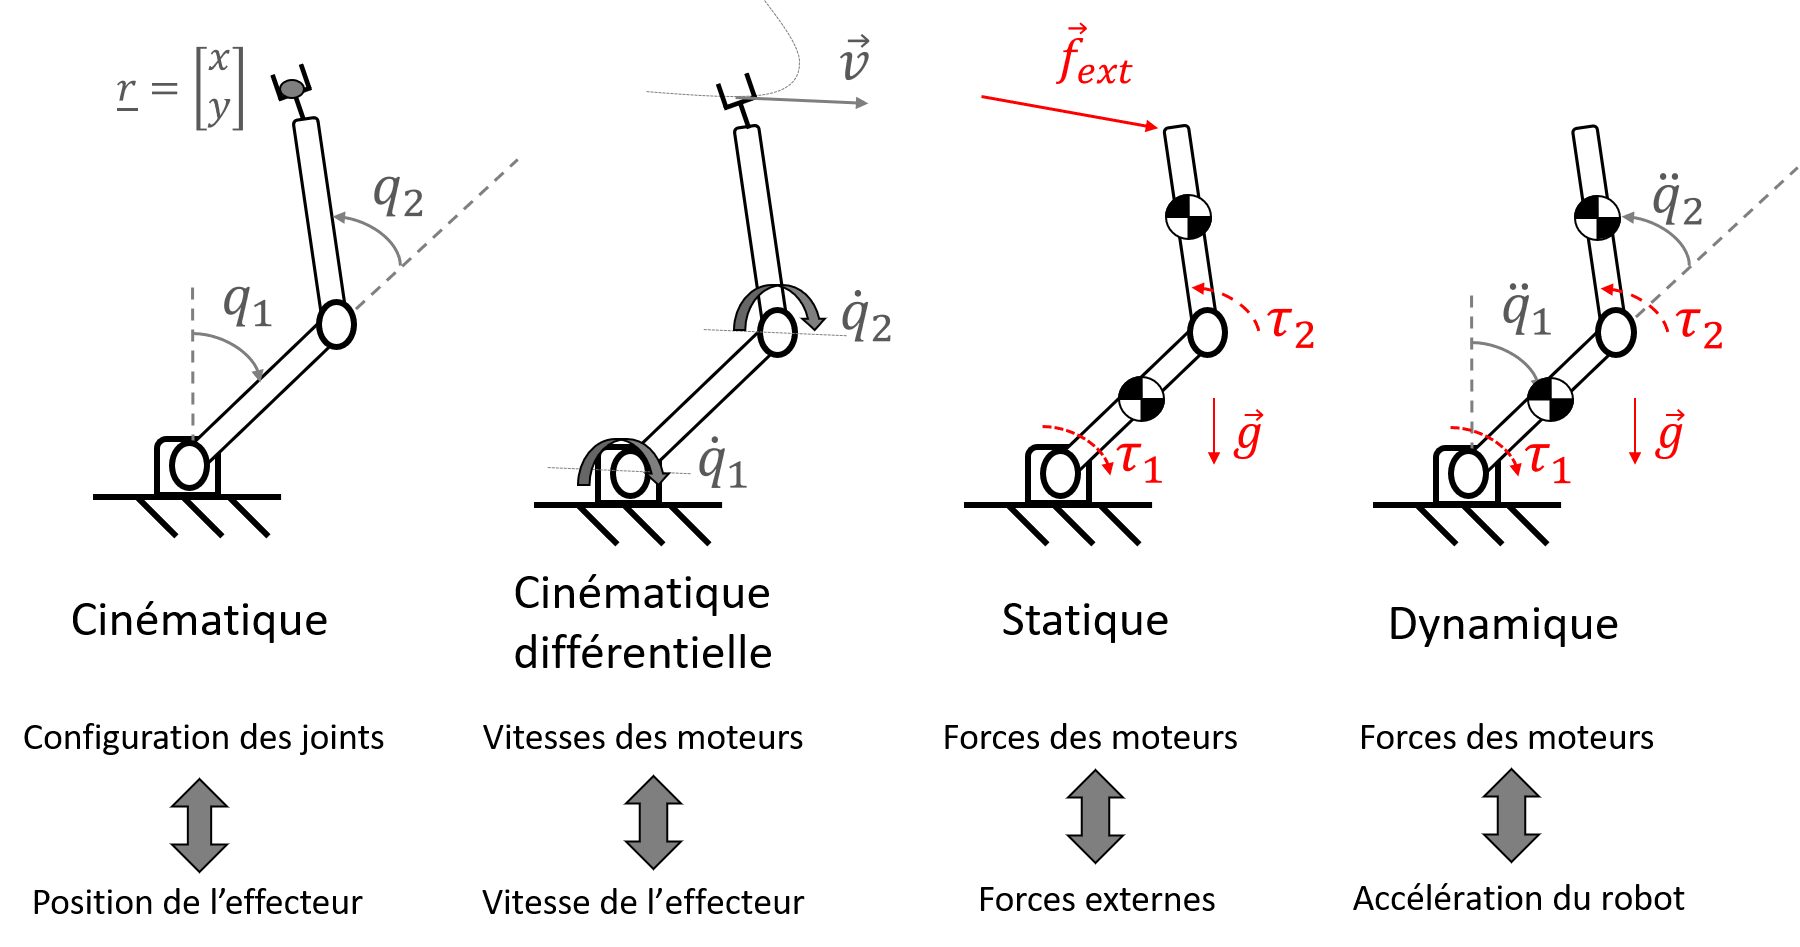
\includegraphics[width=0.95\textwidth]{fields.png}
	\caption{Quatre grands domaines de base de l'analyse de robots manipulateurs  }
	\label{fig:fields}
\end{figure}
%%%%%%%%%%%%%%%%%%%%%%%%%%%%%%%%%%%%%%%%%%%%%%%%%%%%%%%%%%%%%%%%%%%%%%%%%%%%%%%

Les méthodes de \textbf{cinématique directe} visent à calculer la position finale de l'effecteur d'un robot en fonction du positionnement des articulations. Lorsqu'on parle de \textbf{cinématique inverse}, l'objectif est de déterminer le positionnement des articulations qui mène à une position désirée de l'effecteur du robot. Mathématiquement, l'analyse consiste à construire et résoudre la fonction non linéaire qui relie les coordonnées de l'effecteur, groupées dans un vecteur-colonne $\col{r}$, aux coordonnées des joints, groupées dans un vecteur-colonne $\col{q}$:
%%%%%%%%%%%%%%%%
\begin{equation}
	\text{Cinématique directe:}  \quad \col{r} = f\left( \, \col{q} \, \right)  \quad  \text{inverse:} \quad \col{q} = f^{-1}\left( \, \col{r}  \, \right)
\end{equation}
%%%%%%%%%%%%%%%
Un des grands défis est que la fonction inverse $f^{-1}\left( \, \col{r}  \, \right)$ peut avoir plusieurs ou aucune solution, selon les coordonnées de l'effecteur qui sont visées.

Le domaine appelé la \textbf{cinématique différentielle} vise à calculer la vitesse de l'effecteur du robot en fonction de la vitesse des moteurs qui actionnent les articulations, ou vice-versa. Mathématiquement, l'analyse consiste à construire la matrice Jacobienne $J(\col{q})$, qui permet de relier le vecteur-colonne $\col{\dot{r}}$ des vitesses de l'effecteur (la dérivée temporelle des coordonnées $\col{r}$) et le vecteur-colonne $\col{\dot{q}}$ des vitesses des joints (la dérivée temporelle des coordonnées $\col{q}$):
%%%%%%%%%%%%%%%%
\begin{equation}
	\text{Cinématique différentielle directe:} \quad \col{\dot{r}} = J\left( \, \col{q} \, \right) \, \col{\dot{q}}   \quad \text{inverse:} \quad \col{\dot{q}} = J^{\#}\left( \, \col{q} \, \right) \, \col{\dot{r}}
\end{equation}
%%%%%%%%%%%%%%%
Un des défis est que pour certaines configurations du manipulateur la matrice $J(\col{q})$ est singulière, c.-à-d. son inverse $J^{-1}$ n'existe pas. On dit alors que le robot est sur une singularité cinématique où il est impossible de faire bouger l'effecteur dans certaines directions. Un autre défi est que lorsque le nombre de joints est différent du nombre de coordonnées de l'effecteur, la matrice $J$ est rectangulaire et on doit alors utiliser la notion de pseudo-inverse notée $J^{\#}$.

Pour les robots manipulateurs, les analyses de \textbf{statique} visent généralement à déterminer les forces/couples nécessaires aux moteurs/actionneurs d'un robot pour le maintenir en place en fonction des forces externes, ou vice-versa. Mathématique, l'analyse peut aussi utiliser la matrice Jacobienne pour faire la relation entre le vecteur-colonne de couples des moteurs $\col{\tau}$ et le vecteur-colonne des forces externes $\col{f}_{ext}$:
%%%%%%%%%%%%%%%%
\begin{equation}
	\text{Statique:} \quad \col{\tau} = J^T\left( \, \col{q} \, \right) \, \col{f}_{ext}
\end{equation}
%%%%%%%%%%%%%%%

Finalement, la \textbf{dynamique} est le domaine qui vise à déterminer les équations différentielles qui représentent la relation entre l'accélération des joints d'un robot et les forces appliquées. Mathématiquement, l'analyse consiste à construire et analyser une équation différentielle non linéaire (reliant les coordonnées des joints $\col{q}$, la vitesse des joints $\col{\dot{q}}$, l'accélération des joints $\col{\ddot{q}}$, les couples appliqués $\col{\tau}$ et les forces externes $\col{f}_{ext}$) qui prend la forme:
%%%%%%%%%%%%%%%%
\begin{align}
	\text{Dynamique:} \quad H(\col{q}) \col{\ddot{q}} + C(\col{q},\col{\dot{q}}) \col{\dot{q}} + D \col{\dot{q}} + \col{g}(\col{q}) = \col{\tau} - J^T(\col{q}) \, \col{f}_{ext}
	\label{eq:manipulator}
\end{align}
%%%%%%%%%%%%%%%
où les termes $H(\col{q}) \col{\ddot{q}}$ et $C(\col{q},\col{\dot{q}}) \col{\dot{q}}$ représentent des effets inertiels, le terme $D \col{\dot{q}}$ représente des forces dissipatives (ex.: friction) et le terme $\col{g}(\col{q})$ représente des forces gravitationnelles. Cette équation, c'est $\vec{F}=m\vec{a}$ appliqué aux robots manipulateurs.


%%%%%%%%%%%%%%%%%%%%%%%%%%%%%%%%%%%%%%%%%%%%%%%%%%%%%%%%%%%%%%%%%
\note{Hypothèses de travail:}{L'approche de modélisation pour la cinématique, la statique et la dynamique utilisée dans cette partie (chapitres \ref{sec:cine1}, \ref{sec:cinediff}, \ref{sec:static} et \ref{sec:dynamic}) considère les robots comme des systèmes de corps rigides reliés par des articulations qui permettent un nombre restreint de mouvements relatifs. Cette approche de modélisation fait l'hypothèse que \textbf{les déformations des sections rigides du robot sont négligeables}, ce qui est par exemple raisonnable pour les robots manipulateurs industriels dans la plupart des applications.}
%%%%%%%%%%%%%%%%%%%%%%%%%%%%%%%%%%%%%%%%%%%%%%%%%%%%%%%%%%%%%%%%%


\section{L'importance de l'algèbre linéaire pour la robotique}

Contrairement à plusieurs machines et systèmes, les robots sont caractérisés par la présence de plusieurs dimensions. Les entrées sont multiples, par exemple les forces/vitesses des multiples moteurs, et les sorties aussi, par exemple la position $(x,y,z)$ de l'outil. Les quantités intéressantes en robotique (entrées et sorties des analyses) peuvent donc être représentées par des vecteurs-colonne, et les relations entre ceux-ci peuvent être représentées par des opérations matricielles qui simplifient grandement les analyses. L'algèbre linéaire est donc un des outils mathématiques les plus importants pour l'ingénieur roboticien.


\newpage
\section{L'approche présentée dans ces notes}

L'approche de modélisation mise de l'avant dans ces notes se résume à la séquence:
\begin{enumerate}
	\item Décrire le problème avec des vecteurs géométriques symboliques;
	\item Choisir des bases appropriées;
	\item Traduire la relation vectorielle en relation matricielle (projection dans une base);
	\item Déterminer la solution numérique avec les outils de l'algèbre linéaire.
\end{enumerate}

La Figure \ref{fig:approchemodelisation} donne un aperçu de cette approche pour un problème de cinématique directe.

%%%%%%%%%%%%%%%%%%%%%%%%%%%%%%%%%%%%%%%%%%
\begin{figure}[H]
	\centering
	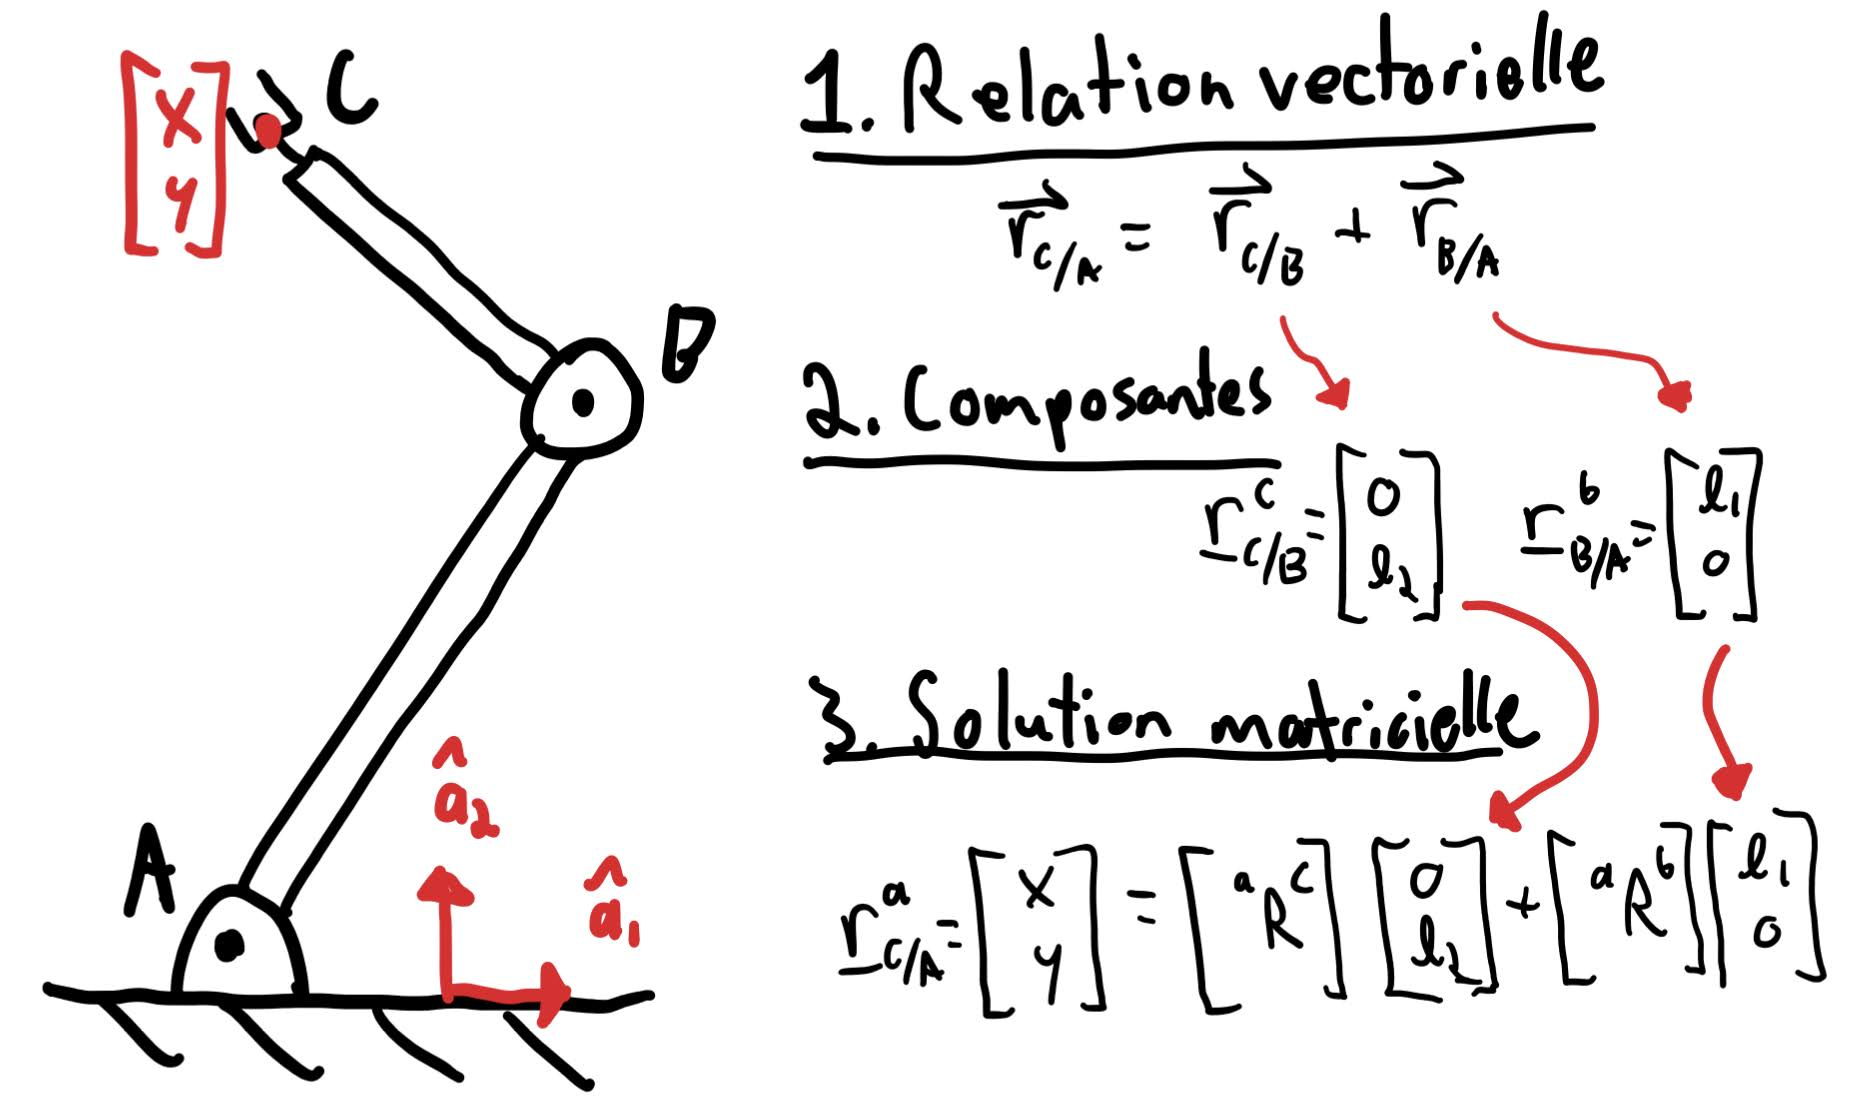
\includegraphics[width=0.7\textwidth]{approchemodelisation.jpg}
	\caption{Aperçu des grandes lignes de l'approche de modélisation présentée dans ces notes}
	\label{fig:approchemodelisation}
\end{figure}
%%%%%%%%%%%%%%%%%%%%%%%%%%%%%%%%%%%%%%%%%%

\section{Organisation des notes de cours (partie \ref{sec:manip})}

Le chapitre \ref{sec:robotmanip} introduit la nomenclature et les concepts de base impliqués dans l'analyse et la modélisation des robots manipulateurs.

Le chapitre \ref{sec:cine1} présente des méthodes mathématiques pour modéliser la cinématique des robots manipulateurs. Premièrement, les systèmes de coordonnées importants pour les robots manipulateurs sont introduits. Ensuite, l'utilisation des vecteurs géométriques, des bases vectorielles et des repères pour représenter la position est présentée. Finalement, ces notions sont appliquées à la résolution des problèmes de cinématique pour les robots manipulateurs.

Le chapitre \ref{sec:cinediff} présente des méthodes pour analyser la cinématique différentielle des robots manipulateurs.

Le chapitre \ref{sec:static} présente des méthodes pour analyser la statique des robots manipulateurs.

Le chapitre \ref{sec:dynamic} présente des méthodes pour analyser la dynamique des robots manipulateurs.

\newpage

\section{Lexique}

\begin{center}
	\begin{tabular}{  p{3.5cm} p{3.5cm} p{7cm} }
%\caption{Définitions techniques }
%\label{def}
		\hline
		\textbf{Terme technique} & \textbf{En anglais} & \textbf{Définition} \\ \hline\hline \\
%%
		Robot Manipulateur &  Manipulator Robot &
		Robot avec une base fixe qui a comme tâche de positionner dans l'espace un objet ou un outil.
		\\  &  \\
		Actionneur &  Actuator &
		Dispositif qui transforme l'énergie en travail mécanique. Typiquement des moteurs électriques et des vérins pneumatiques ou hydrauliques pour les robots.
		\\  &  \\
		Effecteur  & End-effector &
		L'endroit où est situé l'objet ou l'outil manipulé par un robot.
		\\   &  \\
		Corps rigide & Rigid body &
		Un modèle idéal d'un objet qui ne se déforme pas, même lorsque soumis à des forces externes.
		\\   &  \\
		Joint & Joint &
		Jonction mécanique permettant un mouvement relatif entre deux pièces.
		\\  &  \\
		Système de coordonnées &  Coordinate system &
		Ensemble de scalaires (angles ou positions) qui permettent de paramétrer la position/configuration d'un système.
		\\  &  \\
		Degrés-de-Liberté (DDL) & Degree-of-Freedom (DoF) &
		Le nombre de variables indépendantes qui permettent de paramétrer dans l'espace la position/configuration d'un système.
		\\  &  \\
		Base vectorielle  & Vector basis &
		Trois vecteurs unitaires qui définissent une orientation.
		\\  &  \\
		Base vectorielle orthonormée & Orthogonal Vector basis &
		Trois vecteurs unitaires orthogonaux qui définissent une orientation.
		\\  &  \\
		Origine &  Origin &
		Un point de référence pour la mesure des positions.
		\\  &  \\
		Repère &  Frame &
		Combinaison d'une origine et d'une base vectorielle orthonormée.
		\\  &  \\
		Système de coordonnées cartésiennes & Cartesian coordinate system &
		Ensemble de trois scalaires qui déterminent la position d'un point par rapport à une origine et trois axes orthogonaux. %(définis par une base vectorielle orthonormée)
		\\   &  \\
		Référentiel & Reference frame &
		Point de vue choisi pour analyser/observer un mouvement.
		\\  &  \\
		\hline
		\label{tab}
	\end{tabular}
\end{center}

\section{Symboles et notations}

\begin{center}
	\begin{tabular}{p{5cm}  p{9cm}}
%\caption{Nomenclature}
%\label{nom}
		\hline
		\textbf{Symbole} & \textbf{Définition} \\ \hline\hline \\
%%%%%%%%%%%%%%%%%%%%%%%%%%%%%%%%%%%%%%%%%%%%%%%%%%%%%%%%%%%%%%%%%%%%%%%%%%%%%%%%%%%%%%%%%%%%%%%%%%%%
		\multicolumn{2}{l}{Vecteurs géométriques} \\ \hline \\
%%%%%%%%%%%%%%%%%%%%%%%%%%%%%%%%%%%%%%%%%%%%%%%%%%%%%%%%%%%%%%%%%%%%%%%%%%%%%%%%%%%%%%%%%%%%%%%%%%%%
		$\vec{v}$            & Vecteur      \\   &  \\
%%%%%%%%%%%%%%%%%%%%%%%%%%%%%%%%%%%%%%%%%%%%%%%%%%%%%%%%%%%%%%%%%%%%%%%%%%%%%%%%%%%%%%%%%%%%%%%%%%%%
		$\hat{a}$            & Vecteur unitaire   \\   &  \\
%%%%%%%%%%%%%%%%%%%%%%%%%%%%%%%%%%%%%%%%%%%%%%%%%%%%%%%%%%%%%%%%%%%%%%%%%%%%%%%%%%%%%%%%%%%%%%%%%%%%
%$\vec{r}$            & Vecteur position     \\  &  \\
%%%%%%%%%%%%%%%%%%%%%%%%%%%%%%%%%%%%%%%%%%%%%%%%%%%%%%%%%%%%%%%%%%%%%%%%%%%%%%%%%%%%%%%%%%%%%%%%%%%%
%$\vec{a}$            & Vecteur accélération \\   &  \\
%%%%%%%%%%%%%%%%%%%%%%%%%%%%%%%%%%%%%%%%%%%%%%%%%%%%%%%%%%%%%%%%%%%%%%%%%%%%%%%%%%%%%%%%%%%%%%%%%%%%
%$\dot{\vec{r}}$      & Dérivée du vecteur $\vec{r}$ par rapport au temps \\   &  \\
%%%%%%%%%%%%%%%%%%%%%%%%%%%%%%%%%%%%%%%%%%%%%%%%%%%%%%%%%%%%%%%%%%%%%%%%%%%%%%%%%%%%%%%%%%%%%%%%%%%%
%$^{i}\dot{\vec{r}}$  & Dérivée partielle du vecteur $\vec{r}$ par rapport au temps vue dans le référentiel $i$ \\   &  \\
%%%%%%%%%%%%%%%%%%%%%%%%%%%%%%%%%%%%%%%%%%%%%%%%%%%%%%%%%%%%%%%%%%%%%%%%%%%%%%%%%%%%%%%%%%%%%%%%%%%%
		$\vec{r}_{A/B}$      & Vecteur position du point $A$ par rapport au point $B$ \\   &  \\
%%%%%%%%%%%%%%%%%%%%%%%%%%%%%%%%%%%%%%%%%%%%%%%%%%%%%%%%%%%%%%%%%%%%%%%%%%%%%%%%%%%%%%%%%%%%%%%%%%%%
		\multicolumn{2}{l}{Vecteur-colonnes et composantes scalaires} \\ \hline \\
%%%%%%%%%%%%%%%%%%%%%%%%%%%%%%%%%%%%%%%%%%%%%%%%%%%%%%%%%%%%%%%%%%%%%%%%%%%%%%%%%%%%%%%%%%%%%%%%%%%%
		$\col{c} = \left[ \begin{array}{c}
							  c_1 \\ c_2 \\ c_3
		\end{array}  \right] = \left[\begin{array}{ccc} c_1 & c_2 & c_3 \end{array}\right]^T $
		& Vecteur-colonne \\   &  \\
%%%%%%%%%%%%%%%%%%%%%%%%%%%%%%%%%%%%%%%%%%%%%%%%%%%%%%%%%%%%%%%%%%%%%%%%%%%%%%%%%%%%%%%%%%%%%%%%%%%%
%$\col{v}^{T} = \left[v_1,v_2,v_3\right]$
%& Vecteur-rangé  \\   &  \\
%%%%%%%%%%%%%%%%%%%%%%%%%%%%%%%%%%%%%%%%%%%%%%%%%%%%%%%%%%%%%%%%%%%%%%%%%%%%%%%%%%%%%%%%%%%%%%%%%%%%
		$\col{v}^{a}  = \left[ \begin{array}{c}
								   v_1^a \\ v_2^a \\ v_3^a
		\end{array}  \right]$   & Vecteur-colonne des composantes du vecteur $\vec{v}$ dans la base vectorielle $a$  \\   &  \\
%%%%%%%%%%%%%%%%%%%%%%%%%%%%%%%%%%%%%%%%%%%%%%%%%%%%%%%%%%%%%%%%%%%%%%%%%%%%%%%%%%%%%%%%%%%%%%%%%%%%
		$v^{a}_i$        & Composante du vecteur $\vec{v}$ selon le vecteur unitaire $i$ de la base vectorielle $a$ \\   &  \\
%%%%%%%%%%%%%%%%%%%%%%%%%%%%%%%%%%%%%%%%%%%%%%%%%%%%%%%%%%%%%%%%%%%%%%%%%%%%%%%%%%%%%%%%%%%%%%%%%%%%
%%%%%%%%%%%%%%%%%%%%%%%%%%%%%%%%%%%%%%%%%%%%%%%%%%%%%%%%%%%%%%%%%%%%%%%%%%%%%%%%%%%%%%%%%%%%%%%%%%%%
		$\col{q} = \left[ \begin{array}{c}
							  q_1 \\  \vdots \\ q_n
		\end{array}  \right] $            & Vecteur-colonne qui regroupe $n$ scalaires représentant la configuration d'un robot à $n$ DDL dans l'espace des joints. \\   &  \\
%%%%%%%%%%%%%%%%%%%%%%%%%%%%%%%%%%%%%%%%%%%%%%%%%%%%%%%%%%%%%%%%%%%%%%%%%%%%%%%%%%%%%%%%%%%%%%%%%%%%
		\multicolumn{2}{l}{Bases et repères} \\ \hline \\
%%%%%%%%%%%%%%%%%%%%%%%%%%%%%%%%%%%%%%%%%%%%%%%%%%%%%%%%%%%%%%%%%%%%%%%%%%%%%%%%%%%%%%%%%%%%%%%%%%%%
		$\left\{ \hat{a}_1 , \hat{a}_2 , \hat{a}_3 \right\}$  & Base vectorielle $a$ définie par un ensemble de trois vecteurs unitaires orthogonaux \\   &  \\
%%%%%%%%%%%%%%%%%%%%%%%%%%%%%%%%%%%%%%%%%%%%%%%%%%%%%%%%%%%%%%%%%%%%%%%%%%%%%%%%%%%%%%%%%%%%%%%%%%%%
		$\left\{ A_O , \hat{a}_1 , \hat{a}_2 , \hat{a}_3 \right\}$  & Repère $A$ défini par un point d'origine $A_O$ et la base vectorielle $a$ \\   &  \\
%%%%%%%%%%%%%%%%%%%%%%%%%%%%%%%%%%%%%%%%%%%%%%%%%%%%%%%%%%%%%%%%%%%%%%%%%%%%%%%%%%%%%%%%%%%%%%%%%%%%
%%%%%%%%%%%%%%%%%%%%%%%%%%%%%%%%%%%%%%%%%%%%%%%%%%%%%%%%%%%%%%%%%%%%%%%%%%%%%%%%%%%%%%%%%%%%%%%%%%%%
		\multicolumn{2}{l}{Matrices} \\ \hline \\
%%%%%%%%%%%%%%%%%%%%%%%%%%%%%%%%%%%%%%%%%%%%%%%%%%%%%%%%%%%%%%%%%%%%%%%%%%%%%%%%%%%%%%%%%%%%%%%%%%%%
		$M=\left[ \begin{array}{c c c}
					  M_{1,1} & \hdots & M_{1,n}  \\ \vdots & \ddots & \vdots \\ M_{m,1}  & \hdots & M_{m,n}
		\end{array}  \right] $
		& Matrice de $m$ rangées et $n$ colonnes ($m \times n$) \\   &  \\
%%%%%%%%%%%%%%%%%%%%%%%%%%%%%%%%%%%%%%%%%%%%%%%%%%%%%%%%%%%%%%%%%%%%%%%%%%%%%%%%%%%%%%%%%%%%%%%%%%%%
		${}^aR^b = \left[ \begin{array}{c c c}
							  \col{b}_1^a  & \col{b}_2^a & \col{b}_3^a
		\end{array}  \right]$            & Matrice de rotation (3$\times$3) qui représente l'orientation de la base vectorielle $b$ par rapport à la base vectorielle $a$. %Un changement de base est effectué ainsi $ \col{v}^b={}^{b}R^a \col{v}^a$
		\\   &  \\
%%%%%%%%%%%%%%%%%%%%%%%%%%%%%%%%%%%%%%%%%%%%%%%%%%%%%%%%%%%%%%%%%%%%%%%%%%%%%%%%%%%%%%%%%%%%%%%%%%%%
		$^{A}T^B = \left[ \begin{array}{c c}
		{}^aR^b  & \col{r}^a_{B_o/A_o} \\ 0 \; 0 \; 0 & 1
		\end{array}  \right] $           & Matrice de transformation homogène (4$\times$4) du repère $B$ vers le repère $A$\\   &  \\
%%%%%%%%%%%%%%%%%%%%%%%%%%%%%%%%%%%%%%%%%%%%%%%%%%%%%%%%%%%%%%%%%%%%%%%%%%%%%%%%%%%%%%%%%%%%%%%%%%%%
%$\underline{v}^{\times}= \left[ \begin{array}{c c c}
%  0 & -v_3 & v_2  \\ v_3 & 0 & -v_1 \\ -v_2 & v_1 & 0
%\end{array}  \right] $   & Matrice antisymétrique correspondant aux composantes du vecteur $\vec{v}$ pour calculer un %produit vectoriel : $\vec{v} \times \vec{w} \; \leftrightarrow \; \col{v}^{\times}\col{w}$ \\   &  \\
%%%%%%%%%%%%%%%%%%%%%%%%%%%%%%%%%%%%%%%%%%%%%%%%%%%%%%%%%%%%%%%%%%%%%%%%%%%%%%%%%%%%%%%%%%%%%%%%%%%%
		\hline
	\end{tabular}
\end{center}


\chapter{Les robots manipulateurs}
\label{sec:robotmanip}

Les robots manipulateurs correspondent à des bras artificiels, généralement plusieurs liens rigides connectés par des articulations. La grande majorité des robots industriels sont des robots manipulateurs qui ont comme tâche de positionner des outils pour la soudure, la peinture, etc. La figure \ref{fig:nom} présente les composants principaux d'un robot manipulateur. La figure \ref{fig:robotmanipex} illustre des exemples concrets de mécanismes et composants pour un robot manipulateur prototype.

%%%%%%%%%%%%%%%%%%%%%%%%%%%%%%%%%%%%%%%%%%%%%%%%%%%%%%%%%%%%%%%%%%%%%%%%%%%%%
\begin{figure}[H]
	\centering
	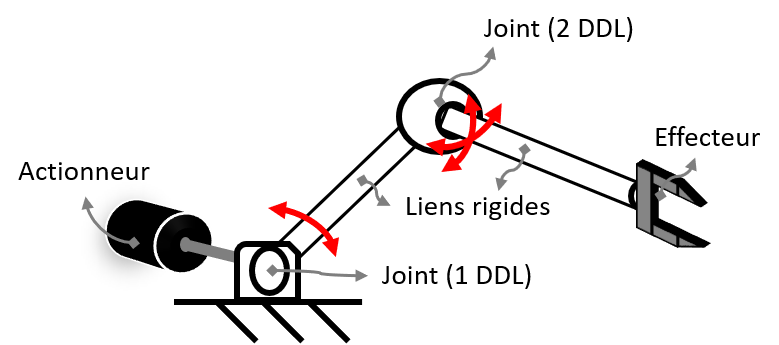
\includegraphics[width=0.55\textwidth]{nom.png}
	\caption{Nomenclature pour l'analyse d'un robot manipulateur}
	\label{fig:nom}
\end{figure}
%%%%%%%%%%%%%%%%%%%%%%%%%%%%%%%%%%%%%%%%%%%%%%%%%%%%%%%%%%%%%%%%%%%%%%%%%%%%%%%

\section{Mécanismes et composants}

Cette section présente les différents composants d'un robot manipulateur ainsi que la nomenclature utilisée.

\subsection{Liens rigides}

Un lien rigide d'un robot, c'est un ensemble de pièces fixes les unes par rapport aux autres qui forment un corps rigide. D'un point de vue de cinématique, deux pièces fixées de telle façon qu'aucun mouvement relatif n'est possible vont être considérées comme un seul lien. Par exemple, plusieurs tubes qui seraient soudés ensemble seraient considérés comme un seul lien rigide.

\subsection{Joints (articulations)}

Les joints sont les articulations d'un robot. Un \textbf{joint prismatique} (articulation linéaire) permet la translation selon un axe entre deux pièces, et contraint les rotations relatives. Un \textbf{joint rotatif} (articulation angulaire) permet à deux pièces de pivoter relativement selon un axe. La variable $q_i$ utilisée pour décrire la configuration d'un joint $i$ est une distance pour un joint prismatique et un angle pour un joint rotatif.
%%%%%%%%%%%%%%%%%%%
\begin{align}
	\text{Joint prismatique:} \quad q_i &= x_i      \quad [m] \\
	\text{Joint rotatif    :} \quad q_i &= \theta_i \quad [rad]
\end{align}
%%%%%%%%%%%%%%%%%%%

Les joints prismatiques et révolus ont une configuration décrite avec une seule variable, chacun des joints de ce type produit donc un degré de liberté (DDL) pour le robot manipulateur. Un robot utilisant seulement ces types de joints a donc un nombre total de DDL qui est égal au nombre de joints. Toutefois, des mécanismes plus complexes (ex.: joint sphérique comme illustré à la figure \ref{fig:nom}) peuvent produire plusieurs DDL en une seule articulation. Par contre, contrairement au corps humain, les robots utilisent généralement des joints prismatiques et rotatifs seulement pour simplifier la mécanique. Un joint sera dit actif si sa configuration est contrôlée par un actionneur, et passif si sa configuration est libre.
%%%%%%%%%%%%%%%%%%%%%%%%%%%%%%%%%%%%%%%%%%%%%%%%%%%%%%%%%%%%%%%
\begin{figure}[H]
	%\vspace{-10pt}
	\centering
	\subfloat[Joint prismatique]{
		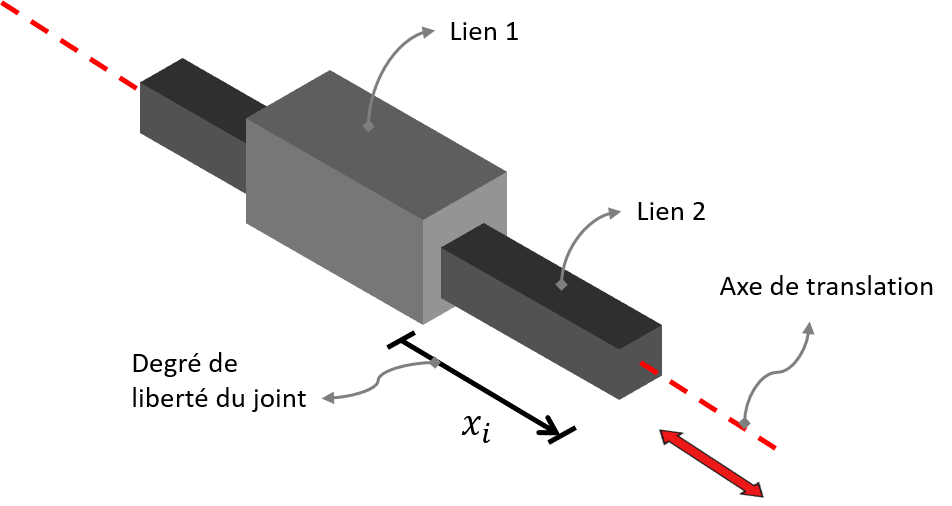
\includegraphics[width=0.48\textwidth]{jointpris}
		\label{fig:jointpris}}
	\subfloat[Joint rotatif]{
		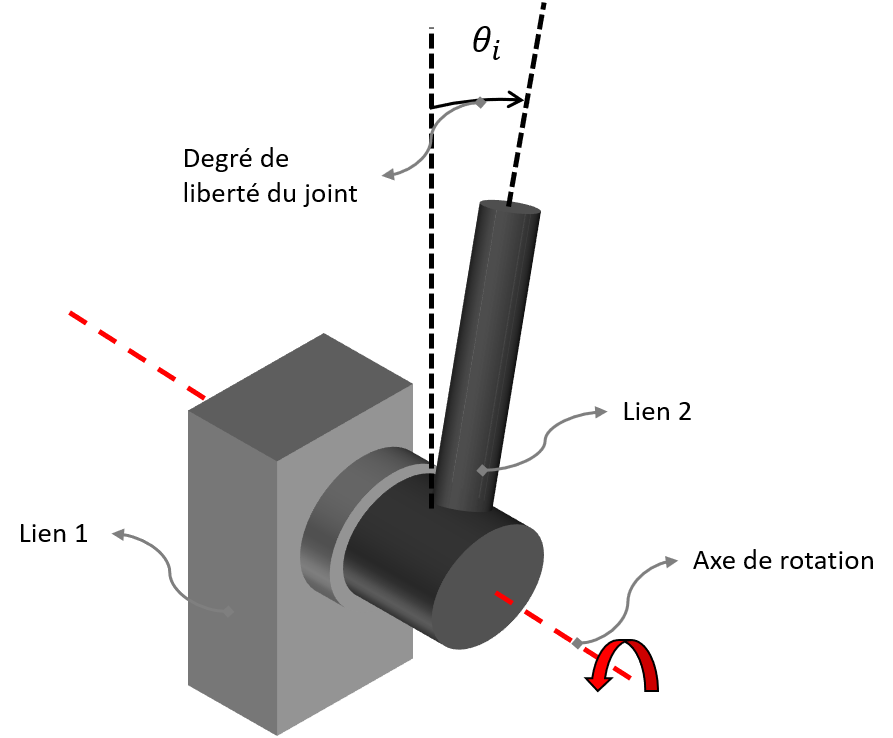
\includegraphics[width=0.48\textwidth]{jointrev}
		\label{fig:jointrev}}
	\caption{Joints à un degré de liberté}
	\label{fig:joint}
\end{figure}
%%%%%%%%%%%%%%%%%%%%%%%%%%%%%%%%%%%%%%%%%%%%%%%%%%%%%%%%%%%%%%%%%

\subsection{Effecteur}

L'effecteur est un terme générique qui réfère à la position de l'outil d'un robot manipulateur (ex.: une pince, une tête de soudure, une caméra, etc.). Dans un espace tridimensionnel, la position d'un objet nécessite au plus six variables pour être complètement décrite (voir section \ref{sec:corps}). L'effecteur d'un robot aura donc au plus 6 DDL.

\subsection{Actionneurs}

Les actionneurs sont les muscles des bras robotiques. Un actionneur est fondamentalement un dispositif qui transforme de l'énergie en travail mécanique. La plupart des robots industriels utilisent des moteurs électriques pour actionner leurs joints, toutefois les actionneurs pourraient aussi être des vérins pneumatiques ou hydrauliques.

\subsection{Capteurs}

Les capteurs sont les dispositifs qui collectent de l'information sur l'état interne d'un robot et/ou l’environnement. Pour la cinématique, les capteurs très régulièrement utilisés sont les encodeurs, qui mesurent directement la position des joints (variables $q_i$), et les systèmes de visions, qui mesurent la position de points dans le repère de la caméra.


%%%%%%%%%%%%%%%
\begin{figure}[htbp]
	\centering
	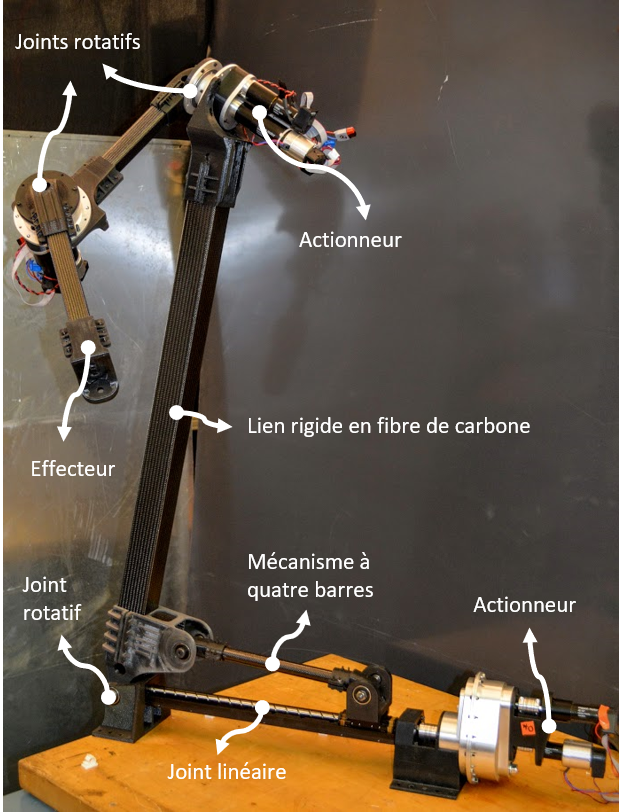
\includegraphics[width=0.80\textwidth]{robotmanipex.png}
	\caption{Prototype de robot manipulateur avec trois degrés de liberté}
	\label{fig:robotmanipex}
\end{figure}
%%%%%%%%%%%%%%%%%


\section{Configurations}

Cette section introduit les notions en lien avec la configuration d'un robot manipulateur.

\subsection{Degrés de liberté}

Le nombre de degrés de liberté (DDL), c'est le nombre de variables nécessaires pour complètement décrire la configuration d'un robot ou un mécanisme. La plupart des robots industriels ont six DDL, ce qui est suffisant pour pouvoir contrôler indépendamment les six DDL de l'effecteur. Pour des robots qui utilisent seulement des joints rotatifs comme illustré à la figure \ref{fig:ddl}, le nombre de DDL est égal au nombre de joints. Si le nombre de DDL est supérieur à six, le robot est dit \textbf{redondant}. Un robot redondant a plusieurs options de configuration des joints pour atteindre une position et une orientation désirées de l'effecteur.

%%%%%%%%%%%%%%%%%%%%%%%%%%%%%%%%%%%%%%%%%%%%%%%%%%%%%%%%%%%%%%%
\begin{figure}[H]
	%\vspace{-10pt}
	\centering
	\subfloat[1 DDL]{
		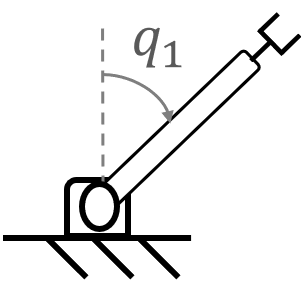
\includegraphics[width=0.20\textwidth]{1ddl}
		\label{fig:1ddl}}
	\subfloat[2 DDL]{
		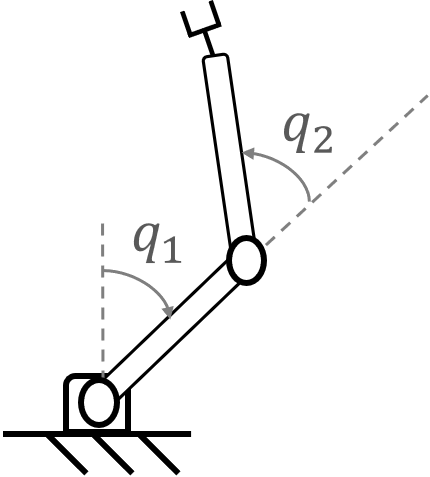
\includegraphics[width=0.25\textwidth]{2ddl}
		\label{fig:2ddl}}
	\subfloat[3 DDL]{
		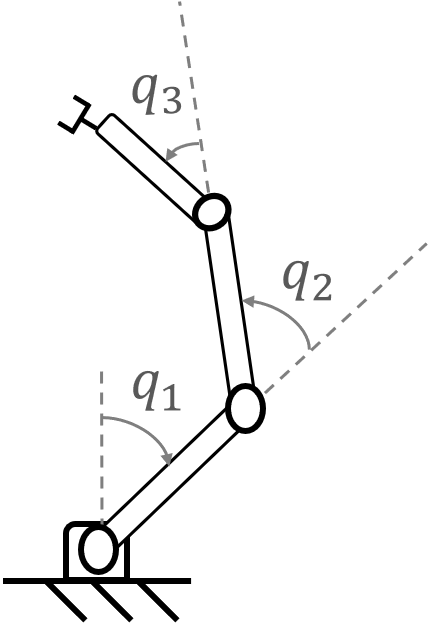
\includegraphics[width=0.25\textwidth]{3ddl}
		\label{fig:3ddl}}
	\caption{Manipulateurs planaires avec des joints rotatifs}
	\label{fig:ddl}
\end{figure}
%%%%%%%%%%%%%%%%%%%%%%%%%%%%%%%%%%%%%%%%%%%%%%%%%%%%%%%%%%%%%%%%%

\subsection{Espace de travail}

L'espace de travail c'est le volume qui comprend toutes les positions atteignables par l'effecteur du robot. La figure \ref{fig:workspace} illustre un espace de travail dans le plan d'un robot à deux joints. Parfois, des sous-ensembles de l'espace de travail peuvent être définis en fonction des positions atteignables avec une orientation précise de l'effecteur.

%%%%%%%%%%%%%%%%%%%%%%%%%%%%%%%%%%%%%%%%%%%%%%%%%%%%%%%%%%%%%%%%%%%%%%%%%%%%%
\begin{figure}[H]
	\centering
	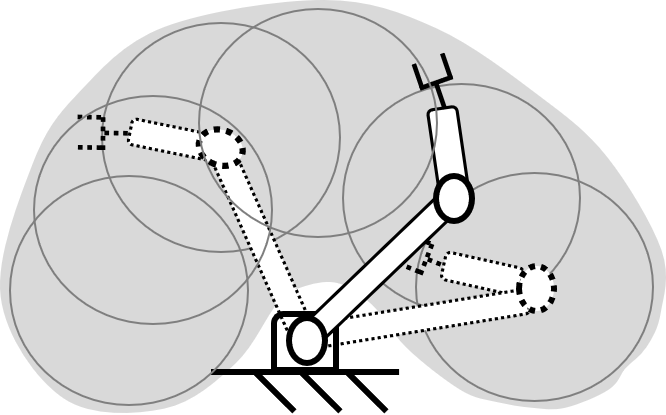
\includegraphics[width=0.45\textwidth]{workspace.png}
	\caption{Exemple de l'espace de travail d'un robot manipulateur à deux joints}
	\label{fig:workspace}
\end{figure}
%%%%%%%%%%%%%%%%%%%%%%%%%%%%%%%%%%%%%%%%%%%%%%%%%%%%%%%%%%%%%%%%%%%%%%%%%%%%%%%

%Parfois, des sous-ensembles de l'espace de travail


%\subsection{Serie vs parallele}




\subsection{Configurations classiques}

À venir!

%scara: https://www.youtube.com/watch?v=vKD20BTkXhk


\chapter{Cinématique I: La position}
\label{sec:cine1}

Ce chapitre présente des méthodes pour modéliser et analyser la position de systèmes à plusieurs degrés de liberté, donc bien adaptés aux robots manipulateurs. Dans un contexte de robotique, les problèmes de cinématique consistent premièrement à bien choisir et définir des systèmes de coordonnées pertinents. Par exemple, des coordonnées généralisées pour décrire la configuration des joints, des coordonnées cartésiennes pour décrire la tâche d'un robot en terme de trajectoire de l'effecteur, des coordonnées sphériques pour décrire les mesures d'un système de vision, etc. Ensuite, le défi est de \textbf{calculer les fonctions de transformations pour passer d'un système de coordonnées à un autre}. Par exemple, pour les robots manipulateurs, le principal défi est le calcul de la fonction de la cinématique directe et son inverse, i.e. une fonction avec comme entrées les coordonnées généralisées qui représentent la configuration des joints et comme sortie la pose de l'effecteur. Le calcul de ces transformations dans un contexte de robotique est le sujet principal de ce chapitre. La section \ref{sec:syscoord} introduit aux différents systèmes de coordonnées. Les sections \ref{sec:vecgeopos} et \ref{sec:basevecpos} introduisent les notions de vecteurs de position géométriques, bases vectorielles et vecteur-colonnes de composantes. Les sections \ref{sec:changematrice} et \ref{sec:repere} présentent les changements de base et les changements des repères. Ensuite, la section \ref{sec:corps} présente les méthodes pour représenter mathématiquement la pose d'un corps rigide. Finalement, les sections \ref{sec:fwdkin} et \ref{sec:invkin} traitent de la cinématique des robots manipulateurs, i.e. le calcul des transformations pour passer de l'espace des joints à la pose de l'effecteur et vice-versa. 

\paragraph{Hypothèses de travail} L'approche utilisée dans ce chapitre considère les robots comme des systèmes de corps rigides reliés par des articulations qui permettent un nombre restreint de mouvements relatifs. Cette approche de modélisation fait l'hypothèse que \textbf{les déformations des sections rigides du robot sont négligeables}, ce qui est par exemple raisonnable pour les robots manipulateurs industriels dans la plupart des applications.  

%%%%%%%%%%%%%%%%%%%%%%%%%%%%%%%%%%%%%%%%%%%%%%%%%%%%%%%%%%%%%

\section{Systèmes de coordonnées}
\label{sec:syscoord}

Un système de coordonnées c'est un ensemble de scalaires, généralement des distances et des angles, qui décrivent la position d'un système. 

%%%%%%%%%%%%%%%%%%%%%%%%%%%%%%%%%%%%%%%%%%%%%%%%%%%
\subsection{Position d'une particule}
\label{sec:syscoordparticule}

Une particule (un point) dans l'espace tri-dimensionnel possède trois DDL et sa position peut donc être complètement déterminée par trois scalaires qui forment un système de coordonnées. Trois types de systèmes de coordonnées sont généralement utilisés pour décrire la position d'une particule par rapport à des axes: \textbf{cartésien} $( x, y, z)$, \textbf{cylindrique} $( r, \theta, z)$ ou \textbf{sphérique} $( \rho, \theta, \phi)$, voir la figure \ref{fig:coorsys}. 

%%%%%%%%%%%%%%%%%%%%%%%%%%%%%%%%%%%%%%%%%%%%%%%%%%%%%%%%%%%%%%%
\begin{figure}[H]
				%\vspace{-10pt}
        \centering
        \subfloat[Cartésien]{
				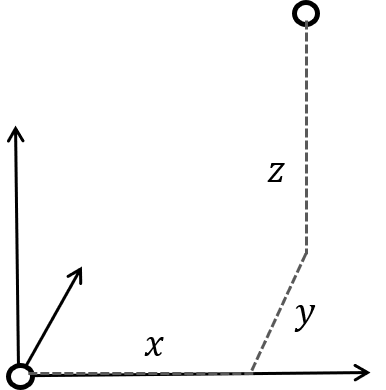
\includegraphics[width=0.28\textwidth]{carsys}
				\label{fig:carsys}}
				\subfloat[Cylindrique]{
				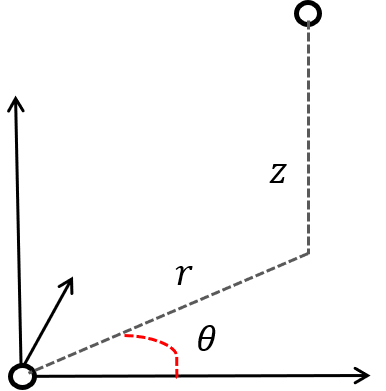
\includegraphics[width=0.28\textwidth]{cylsys}
				\label{fig:cylsys}}
				\subfloat[Sphérique]{
				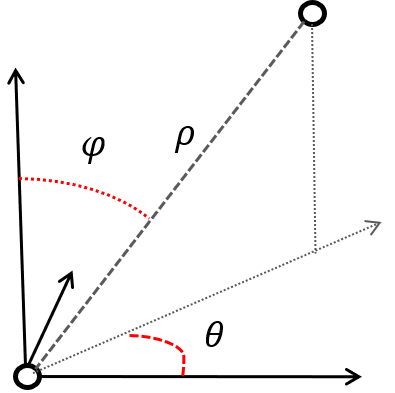
\includegraphics[width=0.28\textwidth]{sphsys}
				\label{fig:sphsys}}
        \caption{Trois systèmes de coordonnées standards pour représenter la position d'un point en 3D}
				\label{fig:coorsys}
\end{figure}
%%%%%%%%%%%%%%%%%%%%%%%%%%%%%%%%%%%%%%%%%%%%%%%%%%%%%%%%%%%%%%%%%

Selon la situation, l'utilisation d'un système de coordonnées particulier peut simplifier l'analyse d'un problème. Par exemple, pour localiser un point géographique sur la Terre, des coordonnées sphériques (ex.: longitude et latitude) sont plus pratiques que des coordonnées cartésiennes ($x$,$y$,$z$) par rapport au centre de la Terre. Parfois l'utilisation d'un type de système de coordonnées est nécessaire car un capteur mesure une coordonnée particulière. Par exemple, le \textit{LIDAR} sur une voiture autonome mesure des distances dans plusieurs directions grâce à un laser pivotant, les données brute sont des coordonnées sphériques. Il est donc parfois inévitable de faire la conversion d'un système de coordonnées à un autre. Le tableau \ref{tab:convcoord} donne les conversions entre des coordonnées cartésiennes, cylindriques et sphériques, qui sont basées sur la même origine et le même système d'axes.
%%%%%%%%%%%%%%%%%%%%%%%%%%%
\begin{table}[htbp]
	\centering
		\begin{tabular}{|p{3cm}|p{3cm}|p{3cm}|p{3cm}|}
		\hline
		 & De cartésien & De cylindrique & De sphérique \\
		\hline 
		 Vers cartésien &
			\vbox{\begin{align*}
			x &= x \\
			y &= y \\
			z &= z
			\end{align*}} 
			& 
			% Polaire vers xyz
			\vbox{\begin{align*}
			x &= r \cos \theta \\
			y &= r \sin \theta \\
			z &= z
			\end{align*}}
			& 
			% Spherical vers xyz
			\vbox{\begin{align*}
			x &= \rho \sin \phi \cos \theta \\
			y &= \rho \sin \phi \sin \theta \\
			z &= \rho \cos \phi
			\end{align*}}
			\\
		\hline
		  Vers cylindrique &
			% xyz vers cylindrique
			\vbox{\begin{align*}
			r &= \sqrt{x^2+y^2} \\
			\theta &= \arctan \frac{y}{x} \\
			z &= z
			\end{align*}}
			&  %cylindrique vers cylindrique
			\vbox{\begin{align*}
			r &= r \\
			\theta &= \theta \\
			z &= z
			\end{align*}}
			& %spherique vers cylindrique
			\vbox{\begin{align*}
			r &= \rho \sin \phi \\
			\theta &= \theta \\
			z &= \rho \cos \phi
			\end{align*}}
			\\
		\hline
		  Vers sphérique &
			% xyz vers Spherical 
			\vbox{\begin{align*}
			\rho &= \sqrt{x^2+y^2+z^2} \\
			\theta &= \arctan \frac{y}{x} \\
			\phi &= \arctan \frac{\sqrt{x^2+y^2}}{z}
			\end{align*}}
			& 
			% cylindrical vers Spherical 
			\vbox{\begin{align*}
			\rho &= \sqrt{r^2+z^2} \\
			\theta &= \theta \\
			\phi &= \arctan \frac{r}{z}
			\end{align*}}
			& 
			%  Spherical 
			\vbox{\begin{align*}
			\rho &= \rho \\
			\theta &= \theta \\
			\phi &= \phi
			\end{align*}}
			\\
		\hline
		\end{tabular}
	\caption{Conversions entre les systèmes de coordonnées cartésiennes, polaires et sphériques qui font référence aux même axes et à la même origine.}
	\label{tab:convcoord}
\end{table}
%%%%%%%%%%%%%%%%%%%%%%%%%%%%%%%%

%%%%%%%%%%%%%%%%%%%%%%%%%%%%%%%%%%%%%%%%%%%
\subsection{Pose d'un corps rigide}
\label{sec:syscoordpose}

Pour décrire la position d'un corps rigide, trois scalaires qui représentent l'orientation sont nécessaires en plus des trois coordonnées qui spécifient la translation, pour un total de six DDL. La combinaison de la translation et de l'orientation est souvent appelée \textbf{la pose} d'un objet. La translation est typiquement spécifiée par la position d'un point sur le corps rigide (ex.: son centre) avec les différentes représentations discutées à la section \ref{sec:syscoordparticule} (cartésienne, cylindrique ou sphérique) et l'orientation est typiquement spécifiée par trois angles. Comme illustré à la figure \ref{fig:pose}, les six coordonnées suivantes pourraient être utilisées pour spécifier la pose d'un objet:
%%%%%%%%%%%%%
\begin{align}
\text{La translation (3 DDL), ex.:} \quad &\left[ x, y, z \right] \\
\text{L'orientation (3 DDL), ex.:} \quad &\left[ \theta_{tangage}, \theta_{roulis}, \theta_{lacet} \right]
\end{align}
%%%%%%%%%%%%%
Il est à noter que \textbf{la représentation de l'orientation d'un corps rigide est un problème complexe} et qu'il existe plusieurs méthodes alternatives pour représenter l'orientation (matrices de rotations, angles de Euler, représentation axe-angle, quaternions, etc.) qui seront discutées à la section \ref{sec:corps}. Selon les domaines (robotique, aérospatiale, engins graphiques des jeux vidéos, vision par ordinateur, astronomie, etc.), différents standards et conventions existent en terme de coordonnées utilisées pour décrire l'orientation. Le point à retenir pour le moment est que trois coordonnées indépendantes sont nécessaires pour représenter une orientation arbitraire, donc six totales sont nécessaires pour représenter une pose arbitraire. Par exemple, un minimum de six coordonnées doivent être utilisées pour: spécifier la position de l'effecteur d'un robot, décrire la position d'un avion dans le ciel, décrire la position de la terre par rapport au soleil, etc. 

\begin{figure}[htbp]
	\centering
		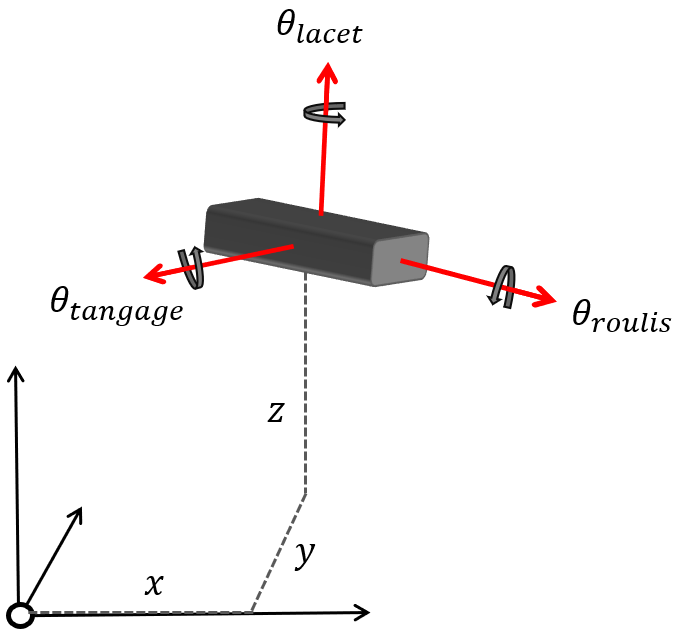
\includegraphics[width=0.50\textwidth]{pose.png}
	\caption{Six coordonnées sont nécessaire pour représenter la pose d'un corps rigide, trois pour décrire la translation et trois pour décrire son orientation.}
	\label{fig:pose}
\end{figure}


%%%%%%%%%%%%%%%%%%%%%%%%%%%%%%%%%%%%%%%%%%%%%%%%%%%%%%
\subsection{Configuration d'un robot manipulateur}
Pour représenter la configuration d'un robot manipulateur il faut suffisamment de variables pour décrire la position relative de chacun des liens rigides qui le compose. Le choix des coordonnées doit être adapté à la géométrie du robot étudié. Un ensemble de variables indépendantes, généralement des angles et des distances, qui permet de déterminer la configuration d'un robot est appelé \textbf{coordonnées généralisées}. L'adjectif \textit{généralisées} est historique et a ici le sens de \textit{pas nécessairement cartésiennes}. Le nombre de coordonnées généralisées nécessaire correspond au nombre de \textbf{degrés-de-liberté} (DDL) du robot.
%\paragraph{Exemples de coordonnées généralisées}
La figure \ref{fig:coor} montre trois exemples de deux coordonnées indépendantes qui peuvent être utilisées comme coordonnées généralisées pour décrire la configuration d'un robot à deux joints rotatifs.

%%%%%%%%%%%%%%%%%%%%%%%%%%%%%%%%%%%%%%%%%%%%%%%%%%%%%%%%%%%%%%%
\begin{figure}[htbp]
				%\vspace{-10pt}
        \centering
        \subfloat[Deux angles relatifs]{
				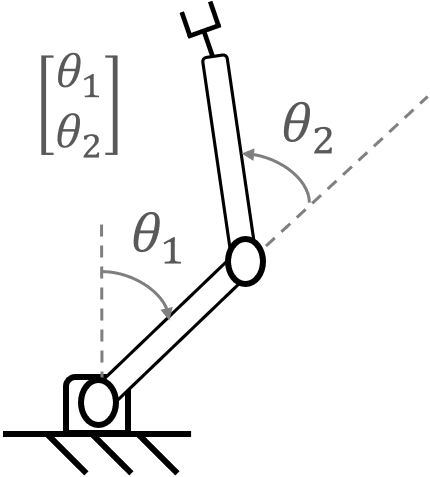
\includegraphics[width=0.24\textwidth]{coor_theta}
				\label{fig:coor_theta}}
				\vspace{10pt}
				\subfloat[Deux angles absolus]{
				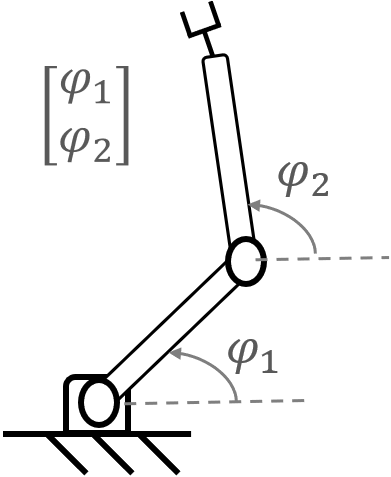
\includegraphics[width=0.22\textwidth]{coor_phi}
				\label{fig:coor_phi}}
				\vspace{10pt}
				\subfloat[Deux distances]{
				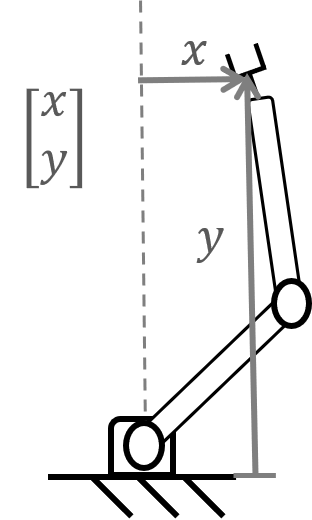
\includegraphics[width=0.18\textwidth]{coor_xy}
				\label{fig:coor_xy}}
				\vspace{-10pt}
        \caption{Trois possibilités de coordonnées indépendantes pour spécifier la position d'un robot à 2 DDL}
				\label{fig:coor}
\end{figure}
%%%%%%%%%%%%%%%%%%%%%%%%%%%%%%%%%%%%%%%%%%%%%%%%%%%%%%%%%%%%%%%%%

%\subsubsection{Espace des joints et espace de la tâche}

\subsubsection{Deux types de systèmes de coordonnées sont généralement utilisés en robotique:}

\paragraph{Espace des joints/actionneurs}

Pour les robots manipulateurs, les algorithmes de contrôle utilisent généralement des coordonnées généralisées qui correspondent à des mesures du déplacement relatif de chaque joint comme illustré à la figure \ref{fig:jointspace}. Ces coordonnées sont généralement notées $\col{q} = \left[ \begin{array}{cccc} q_1 & q_2 & ... & q_n \end{array} \right]^T$ (où $n$ est le nombre de DDL) et on réfère aussi à ce système comme \textbf{l'espace des joints}. Chaque coordonnée $q_i$ représente alors une mesure locale du DDL qui relie deux liens rigides séquentiels. Pour les robots industriels par exemple, ce système de coordonnées est très utile car des encodeurs mesurent directement ces variables et les moteurs les contrôlent de façon indépendante. 

\paragraph{Espace de la tâche}

La tâche d'un robot peut rarement être spécifiée facilement dans l'espace des joints. Un système de coordonnées naturel pour la tâche doit donc généralement être utilisé et on réfère aussi à ce système comme \textbf{l'espace de la tâche}. La tâche d'un robot manipulateur est généralement spécifiée plus naturellement en termes de coordonnées cartésiennes de l'effecteur. Il est à noter que le nombre de coordonnées nécessaires pour l'espace de la tâche peut être différent du nombre de DDL total du robot. Comme illustré à la figure \ref{fig:taskspace}, pour un robot qui aurait comme tâche d'écrire sur une plaque, l'objectif serait naturellement exprimé par une trajectoire définie avec des coordonnées $(x,y)$ sur la plaque. 

%%%%%%%%%%%%%%%%%%%%%%%%%%%%%%%%%%%%%%%%%%%%%%%%%%%%%%%%%%%%%%%
\begin{figure}[htbp]
				%\vspace{-10pt}
        \centering
        \subfloat[Espace des joints]{
				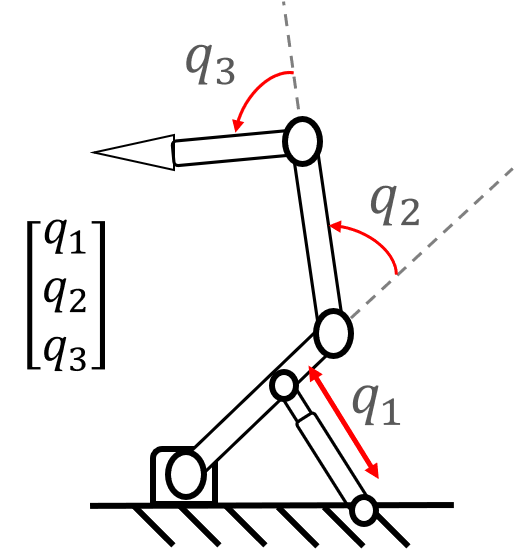
\includegraphics[width=0.28\textwidth]{jointspace}
				\label{fig:jointspace}}
				\hspace{+20pt}
				\subfloat[Espace de la tache]{
				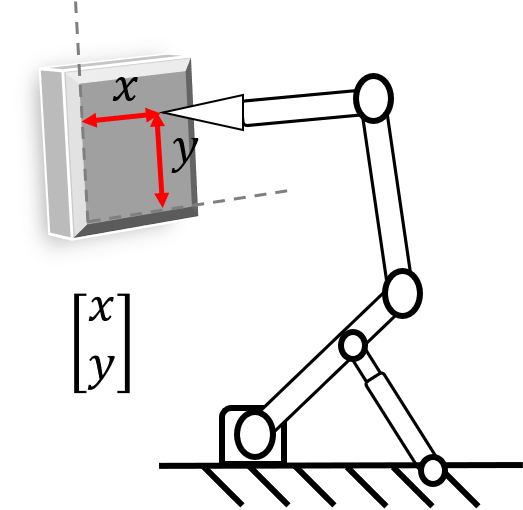
\includegraphics[width=0.28\textwidth]{taskspace}
				\label{fig:taskspace}}
        \caption{Exemple de coordonnées représentant l'espace des joints et l'espace tâche d'un robot manipulateur}
				\label{fig:spaces}
\end{figure}
%%%%%%%%%%%%%%%%%%%%%%%%%%%%%%%%%%%%%%%%%%%%%%%%%%%%%%%%%%%%%%%%%


%%%%%%%%%%%%%%%%%%%%%%%%%%%%%%%%%%%%%%%%%%%%%%%%%%%%%%
%\subsection{Transformation des coordonnées}
%

  



%%%%%%%%%%%%%%%%%%%%%%%%%%%%%%%%%%%%%%%%%%%%%%%%%%%%%%%%%%%%%%%%%%%%%%%%%%%%%%%%%%%%%%%%%%%%%%%%%%%%%%%%%%%%%%%%%%%%%%%%%%%%%%%%%%
\newpage
\section{Vecteurs géométriques de positions}
\label{sec:vecgeopos}

La notion de vecteur géométrique permet de travailler avec des \textbf{vecteurs de position} qui sont indépendants d'un choix de système de coordonnées. Pour les problèmes de cinématique de robots, il est particulièrement adapté de travailler d'abord avec les vecteurs géométrique, plutôt que directement avec des coordonnées. Cette approche \textbf{1)} simplifie les calculs en 3D et \textbf{2)} permet de faire le saut facilement entre plusieurs systèmes de coordonnées. Un vecteur géométrique est une quantité définie dans l’espace et possédant une grandeur et une direction. Dans ces notes, les vecteurs géométriques, notés $\vec{v}$, seront explicitement distingués des vecteur-colonnes (groupe de plusieurs scalaires) qui seront notés $\col{v}=\left[  \begin{array}{ccc} v_{1} & v_{2} & v_{3} \end{array} \right]^T$. 

%La section XXXX présente un rappel sur les propriétés et les opérations possible avec les vecteurs. 

%\subsubsection{Vecteurs de positions}

\textbf{Un vecteur position nécessite deux points pour être défini}, une origine et une destination. Notez que c'est particulier des vecteurs positions, la plupart des autres vecteurs utilisés en physique (vitesse, accélération, force, champ électrique, etc.) ont un point d'application mais sont indépendants d'un choix d’origine. Dans ces notes, les vecteurs positions seront notés:
%%%%%%%%%%%%%%%%%%%%%%%%%%%%%%%%%%%
\begin{equation}
\vec{r}_{B/A}  \quad =  \quad \text{Vecteur position du point $B$ par rapport au point $A$}
\end{equation} 
%%%%%%%%%%%%%%%%%%%%%%%%%%%%%%%%%%%
où $A$ est le point d'origine et $B$ le point de destination, tel qu'illustré à la figure \ref{fig:vecpos}. Parfois, la notation équivalente $\vec{AB}$ est utilisée dans la littérature. Ces vecteurs  peuvent être utilisés pour faire des constructions géométriques indépendamment d'un choix de système de coordonnées. 
%
%%%%%%%%%%%%%%%%%%%%%%%%%%%%%%%%%%%%%%%%%%%%%%%%%%%%%%%%%%%%%%%
\begin{figure}[htb]
				%\vspace{-10pt}
        \centering
				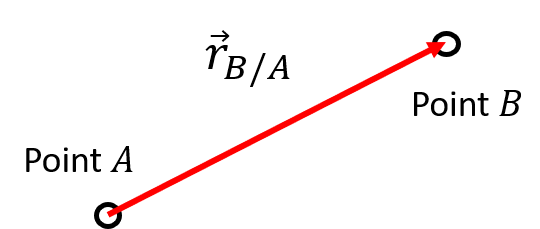
\includegraphics[width=0.30\textwidth]{vecpos}
				\caption{Un vecteur position}
        %\subfloat[Un Vecteur Positions]{
				%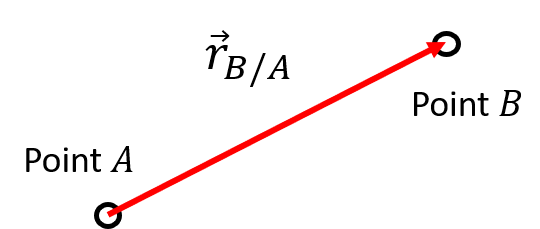
\includegraphics[width=0.30\textwidth]{vecpos}
				%\label{fig:vecpos}}
				%\subfloat[Construction géométrique]{
				%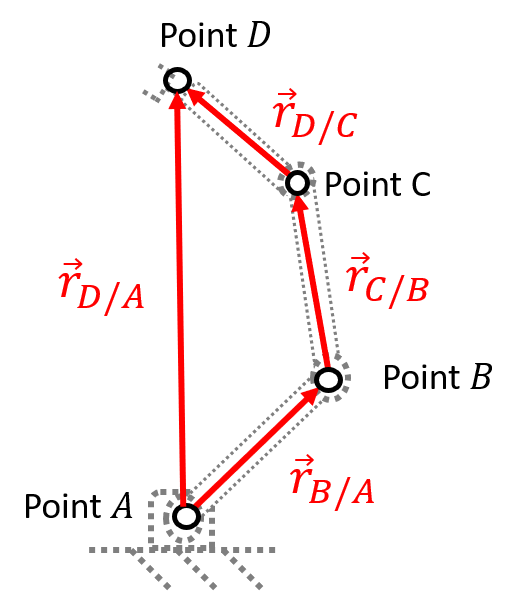
\includegraphics[width=0.30\textwidth]{vecposcons}
				%\label{fig:vecposcons}}
        %\caption{Example de vecteurs de position}
				\label{fig:vecpos}
\end{figure}
%%%%%%%%%%%%%%%%%%%%%%%%%%%%%%%%%%%%%%%%%%%%%%%%%%%%%%%%%%%%%%%%%
%

%%%%%%%%%%%%%%%%%%%%%%%%%%%%%%%%%%%%%%%%%%%%%%%
\subsection{Propriétés des vecteurs de position}
\label{sec:vecposprop}
%
La figure \ref{fig:vecposprop} illustre les propriétés de base des vecteurs de position.
%
%%%%%%%%%%%%%%%%%%%%%%%%%%%%%%%%%%%%%%%%%%%%%%%%%%%%%%%%%%%%%%%
\begin{figure}[htbp]
				%\vspace{-10pt}
        \centering
        \subfloat[Inversion]{
				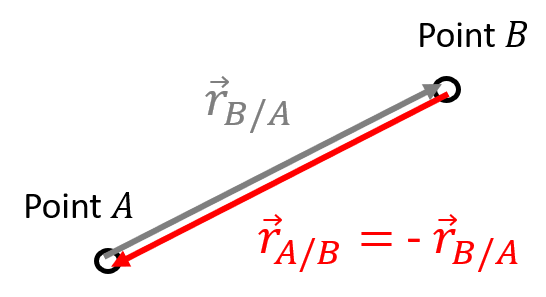
\includegraphics[width=0.28\textwidth]{vecposinv}
				\label{fig:vecposinv}}
				\hspace{5pt}
				\subfloat[Vecteur unitaire et distance]{
				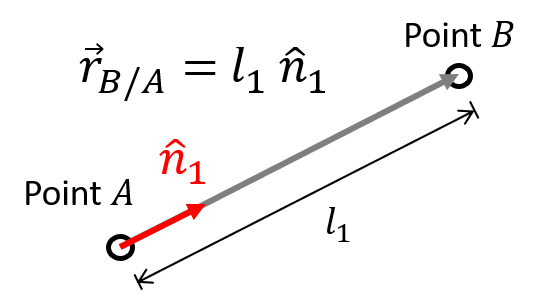
\includegraphics[width=0.28\textwidth]{vecposvecuni}
				\label{fig:vecposinv}}
				\hspace{5pt}
				\subfloat[Addition]{
				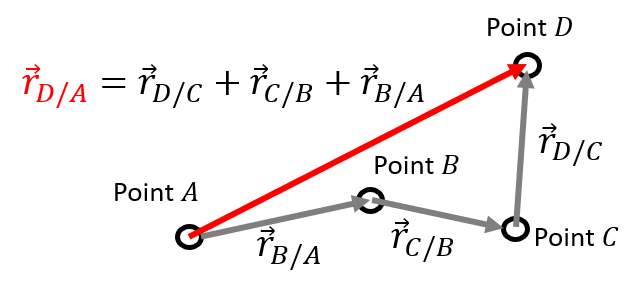
\includegraphics[width=0.35\textwidth]{vecposadd}
				\label{fig:vecposinv}}
				%\vspace{-10pt}
        \caption{Propiétés des vecteurs de position}
				\label{fig:vecposprop}
\end{figure}
%%%%%%%%%%%%%%%%%%%%%%%%%%%%%%%%%%%%%%%%%%%%%%%%%%%%%%%%%%%%%%%%%
%
\paragraph{Addition}
%
Par définition, un vecteur position peut être décomposé en une addition de vecteurs qui passent par des points intermédiaires:
%%%%%%%%%%%%%%%%%%%%%%%%%%%%%%%%%%%
\begin{align}
\vec{r}_{Z/A}  =   \vec{r}_{Z/Y} + \vec{r}_{Y/X} + ... + \vec{r}_{C/B} + \vec{r}_{B/A} 
\end{align} 
%%%%%%%%%%%%%%%%%%%%%%%%%%%%%%%%%%%
%
\paragraph{Inversion}
%
L'inversion de l'origine et la destination est équivalente à la négation du vecteur de position:
%%%%%%%%%%%%%%%%%%%%%%%%%%%%%%%%%%%
\begin{align}
\vec{r}_{B/A}  = - \vec{r}_{A/B}
\end{align} 
%%%%%%%%%%%%%%%%%%%%%%%%%%%%%%%%%%%
%
\paragraph{Vecteurs unitaires}
%
Les vecteurs unitaires sont utilisés pour représenter des directions dans l'espace. Les vecteurs positions peuvent être exprimés comme des \textbf{combinaisons de distances et directions} qui sont représentées respectivement par des paires de scalaires $l_i$ et vecteurs unitaires $\hat{n}_i$:
%%%%%%%%%%%%%%%%%%%%%%%%%%%%%%%%%%%
\begin{equation}
\vec{r} = l_1 \hat{n}_1 + l_2 \hat{n}_2 + ... + l_n \hat{n}_n
\end{equation} 
%%%%%%%%%%%%%%%%%%%%%%%%%%%%%%%%%%%
%Des vecteurs unitaires doivent être identifiés selon les axes pertinents pour l'analyse d'un problème. 



%%%%%%%%%%%%%%%%%%%%%%%%%%%%%%%%%%%%%%%%%%%%%%%
\subsection{Mesures avec les vecteurs de position}
\label{sec:vecuni}
%
%Les vecteurs unitaires sont aussi utiles pour pouvoir mesurer une position selon une direction particulière. 
La norme d'un vecteur position, i.e. sa longueur, peut être calculée en effectuant un produit scalaire du vecteur avec lui même:
%%%%%%%%%%%%%%%%%%%%%%%%%%%%%%%%%%%
\begin{equation}
\| \vec{r} \|^2 = \vec{r} \bullet \vec{r} 
\label{eq:dotnorm}
\end{equation} 
%%%%%%%%%%%%%%%%%%%%%%%%%%%%%%%%%%%
Aussi, la dimension $d$ d'un vecteur position $\vec{r}$ selon un axe particulier correspond au produit scalaire du vecteur position avec un vecteur unitaire $\hat{n}$ aligné sur cet axe:
%%%%%%%%%%%%%%%%%%%%%%%%%%%%%%%%%%%
\begin{equation}
d = \vec{r} \bullet \hat{n} = \| \vec{r} \|  \cos \angle (\vec{r},\hat{n})
\label{eq:vecproj}
\end{equation} 
%%%%%%%%%%%%%%%%%%%%%%%%%%%%%%%%%%%
Cette opération est aussi appelée \textbf{projection d'un vecteur sur un axe} et illustrée à la figure \ref{fig:distproj}. Finalement, le produit scalaire de deux vecteurs unitaires est égale au cosinus de l'angle qui les sépare puisqu'ils ont une dimension unitaire:
%%%%%%%%%%%%%%%%%%%%%%%%%%%%%%%%%%%
\begin{equation}
\cos \angle (\hat{n}_1,\hat{n}_2) =  \hat{n}_1 \bullet \hat{n}_2
\label{eq:dotangle}
\end{equation} 
%%%%%%%%%%%%%%%%%%%%%%%%%%%%%%%%%%%
Il est donc possible d'utiliser le produit scalaire pour mesurer un angle entre deux vecteurs, comme illustré à la figure \ref{fig:dotcosuni}.  
%
%%%%%%%%%%%%%%%%%%%%%%%%%%%%%%%%%%%%%%%%%%%%%%%%%%%%%%%%%%%%%%%
\begin{figure}[htbp]
				%\vspace{-10pt}
        \centering
        \subfloat[Distance selon un axe]{
				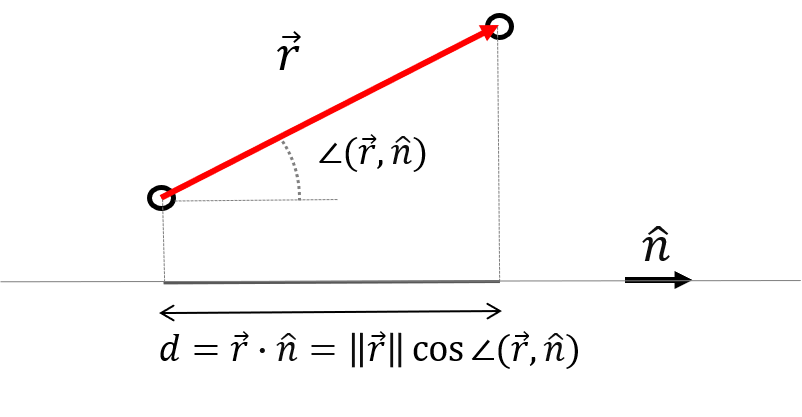
\includegraphics[width=0.40\textwidth]{distproj}
				\label{fig:distproj}}
				\hspace{20pt}
				\subfloat[Angle entre deux vecteurs unitaires]{
				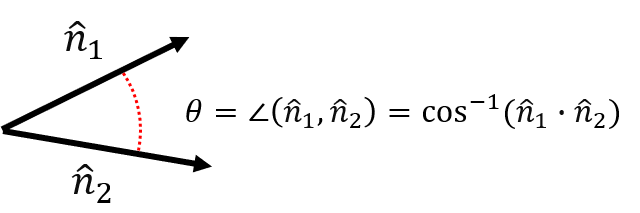
\includegraphics[width=0.35\textwidth]{dotcosuni}
				\label{fig:dotcosuni}}
        \caption{Utilisation du produit scalaire pour des mesures géométriques}
				\label{fig:utprosca}
\end{figure}
%%%%%%%%%%%%%%%%%%%%%%%%%%%%%%%%%%%%%%%%%%%%%%%%%%%%%%%%%%%%%%%%%
%TODO ajouter figure pour la norme

\subsection{Exemple: calcul de la hauteur d'un robot}
\label{sec:hauteurrobot}
%
Un exemple est ici donné pour le calcul de la hauteur de l'effecteur d'un robot à 3 DDL, illustré à la figure \ref{fig:vecposphi}, avec l'aide des vecteurs géométriques de position. Comme illustré à la Figure \ref{fig:vecposcons}, par inspection il est possible de déterminer la relation vectorielle suivante:
%%%%%%%%%%%%%%%%%%%%%%%%%%%%%%%%%%%
\begin{equation}
\vec{r}_{D/A} = \vec{r}_{D/C} + \vec{r}_{C/B} + \vec{r}_{B/A}
\label{eq:vecadd}
\end{equation} 
%%%%%%%%%%%%%%%%%%%%%%%%%%%%%%%%%%%
Ensuite, comme illustré à la figure \ref{fig:vecposuni}, des vecteurs unitaires $\hat{n}_i$ alignés avec chacun des liens rigides du robot manipulateur permettent de préciser l'équation \eqref{eq:vecadd} avec des longueurs et des directions:
%%%%%%%%%%%%%%%%%%%%%%%%%%%%%%%%%%%
\begin{equation}
\vec{r}_{D/A} = l_1 \hat{n}_{1} + l_2 \hat{n}_{2} + l_3 \hat{n}_{3}
\label{eq:vecadduni}
\end{equation} 
%%%%%%%%%%%%%%%%%%%%%%%%%%%%%%%%%%%
Finalement, pour calculer la hauteur $h$ de ce robot par exemple, il suffit de prendre le produit scalaire avec un vecteur unitaire vertical $\hat{y}$:
%%%%%%%%%%%%%%%%%%%%%%%%%%%%%%%%%%%
\begin{align}
h &= \vec{r}_{D/A} \bullet \hat{y} \\
h &= ( l_1 \hat{n}_{1} + l_2 \hat{n}_{2} + l_3 \hat{n}_{3} ) \bullet \hat{y} \\
h &= l_1 ( \hat{n}_{1} \bullet \hat{y} ) + l_2 ( \hat{n}_{2} \bullet \hat{y} ) + l_3 ( \hat{n}_{3}  \bullet \hat{y} ) \\
h &= l_1 \cos \angle (\hat{n}_{1},\hat{y}) + l_2 \cos \angle (\hat{n}_{2},\hat{y}) + l_3 \cos \angle (\hat{n}_{3},\hat{y})
\label{eq:vecaddproj}
\end{align} 
%%%%%%%%%%%%%%%%%%%%%%%%%%%%%%%%%%%
À noter ici que le produit scalaire de deux vecteurs unitaires correspond au cosinus de l'angle entre les deux vecteurs, voir équation \eqref{eq:dotangle}. Donc avec l’exemple ci-dessus le produit scalaire $\hat{n}_{i} \bullet \hat{y}$ correspond simplement au cosinus de l'angle du joint $i$ avec l'axe vertical, donné par les angles $\varphi_i$ à la figure \ref{fig:vecposphi}. L'équation \eqref{eq:vecaddproj} peut donc être précisée comme une expression des variables de distances $l_i$ et des variables d'angles $\varphi_i$: 
%%%%%%%%%%%%%%%%%%%%%%%%%%%%%%%%%%%
\begin{align}
h &= l_1 \cos (\varphi_1) + l_2 \cos (\varphi_2) + l_3 \cos (\varphi_3)
\label{eq:vecaddprojphi}
\end{align} 
%%%%%%%%%%%%%%%%%%%%%%%%%%%%%%%%%%%
Dans un cas simple planaire comme celui-ci il aurait été assez simple de calculer la hauteur du robot directement par trigonométrie. L'approche vectorielle est toutefois plus systématique et se généralise beaucoup plus facilement à des systèmes complexes et tri-dimensionnels comme les robots industriels.
%
%%%%%%%%%%%%%%%%%%%%%%%%%%%%%%%%%%%%%%%%%%%%%%%%%%%%%%%%%%%%%%%
\begin{figure}[H]
				%\vspace{-10pt}
        \centering
				%%%
        \subfloat[Robot à 3 DLL]{
				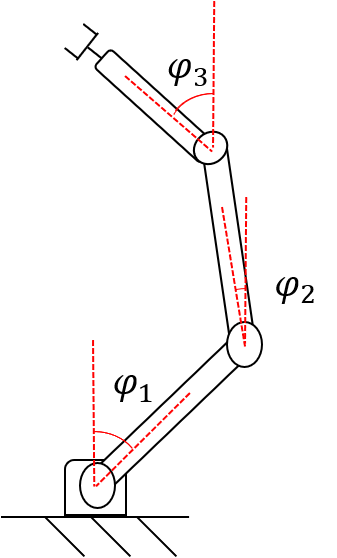
\includegraphics[width=0.17\textwidth]{vecposphi}
				\label{fig:vecposphi}}
				%%%%%%%%%%%%%%%%%%
				\hspace{3pt}
				%%%%
				\subfloat[Vecteurs géométrique]{
				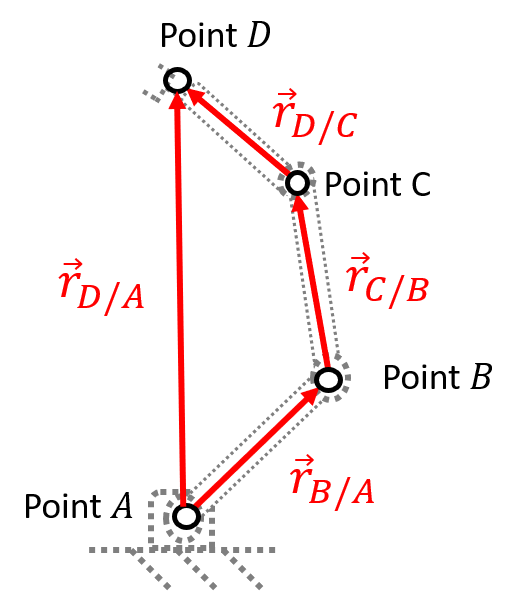
\includegraphics[width=0.26\textwidth]{vecposcons}
				\label{fig:vecposcons}}
				%%%%
				\hspace{3pt}
				%%%%
        \subfloat[Vecteur unitaires]{
				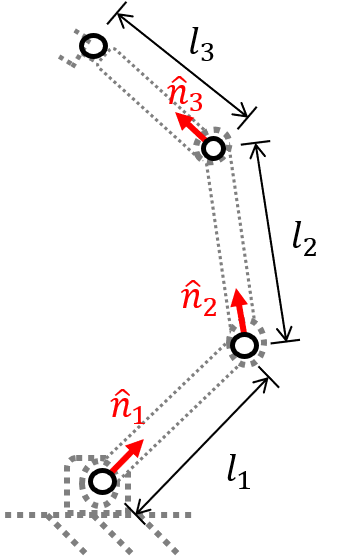
\includegraphics[width=0.17\textwidth]{vecposuni}
				\label{fig:vecposuni}}
				%%%%
				\hspace{3pt}
				%%%%
				\subfloat[Projection sur l'axe vertical]{
				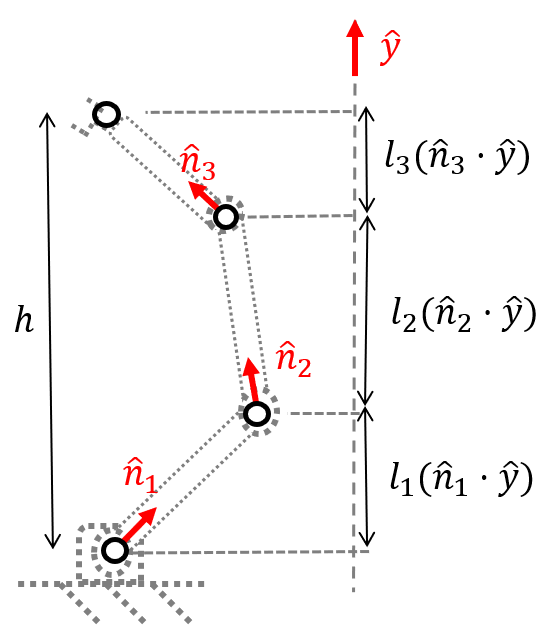
\includegraphics[width=0.29\textwidth]{vecpospro}
				\label{fig:vecpospro}}
        \caption{Exemple de calcul de la hauteur d'un robot.}
				\label{fig:vecposunipro}
\end{figure}
%%%%%%%%%%%%%%%%%%%%%%%%%%%%%%%%%%%%%%%%%%%%%%%%%%%%%%%%%%%%%%%%%

%TODO, faire exemple 3D vectoriel ici


\subsection{Procédure d'utilisation pour le calcul de distances}
La démarche utilisée pour calculer des positions avec les vecteurs géométriques se résume par les trois étapes suivantes:
\begin{enumerate}
	\item Par inspection, construire le vecteur position $\vec{r}$ d’intérêt comme une addition/soustraction de plusieurs vecteurs positions $\vec{r}_i$ avec des longueurs et orientations connues:
	%%%%%%%%%%%%%%%%%%%%%%%%%%%%%%%%%%%
	\begin{equation}
	\vec{r} = \sum_i \vec{r}_i
	\end{equation} 
	%%%%%%%%%%%%%%%%%%%%%%%%%%%%%%%%%%%
	\item Substituer les vecteurs positions symboliques $\vec{r}_i$ par des variables de distance $l_i$ et des vecteurs unitaires $\hat{n}_i$ représentant des directions qui peuvent être mesurées:
	%%%%%%%%%%%%%%%%%%%%%%%%%%%%%%%%%%%
	\begin{equation}
	\vec{r} = \sum_i l_i \hat{n}_i
	\end{equation} 
	%%%%%%%%%%%%%%%%%%%%%%%%%%%%%%%%%%%
	\item Calculer les distances désirées $d$ en effectuant un produit scalaire avec les vecteurs unitaires selon les axes désirés:
	%%%%%%%%%%%%%%%%%%%%%%%%%%%%%%%%%%%
	\begin{align}
	d_x = \vec{r} \bullet \hat{x} = \sum_i l_i ( \hat{n}_i \bullet \hat{x} ) =  \sum_i l_i \cos \angle (\hat{n}_{i},\hat{x}) \\ 
	d_y = \vec{r} \bullet \hat{y} = \sum_i l_i ( \hat{n}_i \bullet \hat{y} ) =  \sum_i l_i \cos \angle (\hat{n}_{i},\hat{y}) \\ 
	d_z = \vec{r} \bullet \hat{z} = \sum_i l_i ( \hat{n}_i \bullet \hat{z} ) =  \sum_i l_i \cos \angle (\hat{n}_{i},\hat{z}) 
	\end{align} 
	%%%%%%%%%%%%%%%%%%%%%%%%%%%%%%%%%%%
\end{enumerate}





%%%%%%%%%%%%%%%%%%%%%%%%%%%%%%%%%%%%%%%%%%%%%%%%%%%%%%%%%%%%%%%%%%%%%%%%%%%%%%%%%%%%%%%%%%%%%%%%%%%%%%%%%%%%%%%%%%%%%%%%%%%%%%%%%%
\newpage
\section{Bases vectorielles et composantes d'un vecteur position}
\label{sec:basevecpos}

Les vecteurs positions tri-dimensionnels $\vec{r}$ peuvent être décris par trois scalaires qui représentent des distances ($r_1$, $r_2$ et $r_3$) qui multiplient trois vecteur unitaires orthogonaux ($\hat{a}_1$, $\hat{a}_2$ et $\hat{a}_3$) qui forment une base vectorielle.  Les scalaires $r_i$ qui multiplient chaque vecteur unitaire sont appelés composantes et peuvent être regroupés sous la forme d'un vecteur-colonne, la notation suivante sera utilisée:
%%%%%%%%%%%%%%%%%%%%%%%%%%%%%%%%%%%
\begin{equation}
\text{Vecteur géométrique:}\quad
\vec{r} = r_1^a \, \hat{a}_{1} + r_2^a \, \hat{a}_{2} + r_3^a \, \hat{a}_{3}
\quad \quad 
\text{Vecteur-colonne:}\quad
\col{r}^{a} = \left[ \begin{array}{c} r_1^a \\ r_2^a \\ r_3^a  \end{array} \right] 
\label{eq:veccoldef}
\end{equation} 
%%%%%%%%%%%%%%%%%%%%%%%%%%%%%%%%%%%
où l'exposant $a$ est utilisé pour spécifier la base vectorielle associée aux composantes scalaires. 




%%%%%%%%%%%%%%%%%%%%%%%%%%%%%%%%%%%%%%%%%%
\subsection{Les bases vectorielles}
Une base vectorielle correspond à trois vecteurs unitaires (en 3D) orthogonaux qui déterminent l'orientation de trois axes dans l'espace et forment une base qui permet de décrire n'importe quel vecteur $\vec{v}$ sous la forme:
%%%%%%%%%%%%%%%%%%%%%%%%%%%%%%%%%%%
\begin{equation}
\vec{v} = v_1^a \, \hat{a}_{1} + v_2^a \, \hat{a}_{2} + v_3^a \, \hat{a}_{3}
\label{eq:vecbasis}
\end{equation} 
%%%%%%%%%%%%%%%%%%%%%%%%%%%%%%%%%%%
On appellera \textit{base vectorielle} $a$, une base formée par l'ensemble des vecteurs unitaires $\{\hat{a}_{1},\hat{a}_{2},\hat{a}_{3}\}$.
%
%%%%%%%%%%%%%%%%%%%%%%%%%%%%%%%%%%%%%%%%%%%%%%%%%%%%%%%%%%%%%%%
\begin{figure}[htpb]
				%\vspace{-10pt}
        \centering
				\subfloat[Base $a$]{
				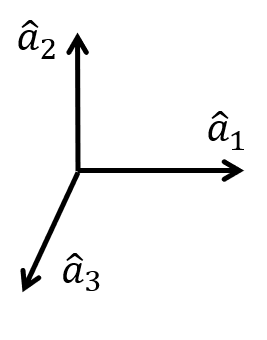
\includegraphics[width=0.20\textwidth]{base}
				\label{fig:base}}
				%%%%
				\hspace{10pt}
				%%%%
        \subfloat[Exemple]{
				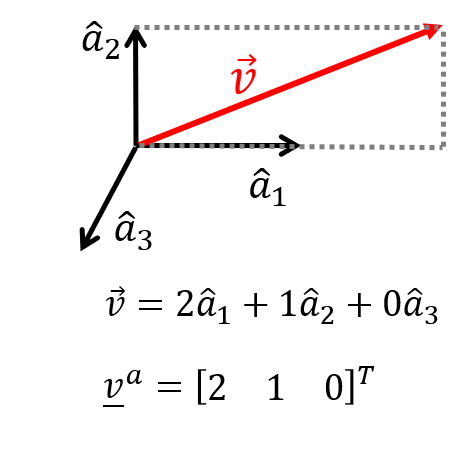
\includegraphics[width=0.25\textwidth]{baseex}
				\label{fig:baseex}}
				%%%%
				\hspace{10pt}
				%%%%
				\subfloat[Convention de la main droite]{
				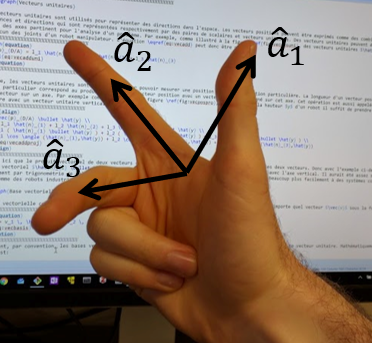
\includegraphics[width=0.25\textwidth]{righthand}
				\label{fig:righthand}}
        \caption{Les bases vectorielles}
				\label{fig:vecbasis}
\end{figure}
%%%%%%%%%%%%%%%%%%%%%%%%%%%%%%%%%%%%%%%%%%%%%%%%%%%%%%%%%%%%%%%%%

Mathématiquement, les critères de dimensions unitaires et d'orthogonalités sont donnés par les équations:
%%%%%%%%%%%%%%%%%%%%%%%%%%%%%%%%%%%
\begin{align}
\hat{a}_{1} \bullet \hat{a}_{1} = 1 \quad\quad \hat{a}_{2} \bullet \hat{a}_{2} = 1 \quad\quad \hat{a}_{3} \bullet \hat{a}_{3} = 1 
\label{eq:unit} \\
\hat{a}_{1} \bullet \hat{a}_{2} = 0 \quad\quad \hat{a}_{2} \bullet \hat{a}_{3} = 0 \quad\quad \hat{a}_{3} \bullet \hat{a}_{1} = 0
\label{eq:ortho}
\end{align} 
%%%%%%%%%%%%%%%%%%%%%%%%%%%%%%%%%%%
Normalement, par convention, les bases vectorielles suivent la règle de main droite (voir figure \ref{fig:righthand}) pour spécifier la direction du troisième vecteur unitaire. La convention de la main droite permet aussi de spécifier des relations en termes de produits vectoriels entre les vecteurs unitaires:
%%%%%%%%%%%%%%%%%%%%%%%%%%%%%%%%%%%
\begin{align}
\hat{a}_{1} = \hat{a}_{2} \times \hat{a}_{3} \quad\quad \hat{a}_{2} = \hat{a}_{3} \times \hat{a}_{1} \quad\quad \hat{a}_{3} = \hat{a}_{1} \times \hat{a}_{2} 
\label{eq:righthand}
\end{align} 
%%%%%%%%%%%%%%%%%%%%%%%%%%%%%%%%%%%

Les bases vectorielles permettent de faire des opérations et combiner des vecteurs en les exprimant avec une base commune de vecteurs unitaires. Dans la littérature, la notation $(\hat{i},\hat{j},\hat{k})$ ou $(\hat{x},\hat{y},\hat{z})$ est parfois utilisée. Dans ces notes, on utilisera des lettres ($a$,$b$,$c$,...) pour identifier des bases, ainsi que des indices (1,2,3) pour spécifier les trois axes (voir figure \ref{fig:base}). Cette approche simplifie la notation lorsqu'un grand nombre de bases sont utilisées simultanément, comme c'est souvent le cas en robotique.

\paragraph{Note:} Les bases vectorielles représentent seulement des orientations, la position d'une base est donc sans signification. Dans les dessins et schémas, on dessine une base vectorielle sur un corps rigide pour signifier que celle-ci est attachée au corps rigide et tourne avec celui-ci, toutefois la position de la base vectorielle sur le corps est arbitraire. On parlera de repère, voir section \ref{sec:repere}, lorsqu'un point d'origine est associé à une base vectorielle. 




%%%%%%%%%%%%%%%%%%%%%%%%%%%%%%%%%%%%%%%%%%%%%%%
\subsection{Relations entre le vecteur géométrique et le vecteur-colonne}

Comme illustré à la figure \ref{fig:vecpospro2}, il est possible de calculer les composantes d'un vecteur exprimé dans une base par un produit scalaire du vecteur géométrique avec chacun des vecteurs unitaires de la base:
%%%%%%%%%%%%%%%%%%%%%%%%%%%%%%%%%%%
\begin{equation}
r_i^a = \vec{r} \bullet \hat{a}_i  \quad \Rightarrow \quad 
\col{r}^{a} = \left[ \begin{array}{c} \vec{r} \bullet \hat{a}_1 \\ \vec{r} \bullet \hat{a}_2 \\ \vec{r} \bullet \hat{a}_3  \end{array} \right] 
\end{equation} 
Inversement, comme illustré à la figure \ref{fig:vecpospro3}, le vecteur position géométrique peut être reconstruit en effectuant la somme des composantes multipliées avec leurs vecteurs unitaires respectifs:
%%%%%%%%%%%%%%%%%%%%%%%%%%%%%%%%%%%
\begin{equation}
\vec{r} = \sum_{i} r_i^a \hat{a}_i = r_1^a \hat{a}_1 + r_2^a \hat{a}_2 + r_3^a \hat{a}_3%= \left[ \begin{array}{c c c} p_1^a & p_2^a & p_3^a  \end{array} \right]  \left[ \begin{array}{c} \hat{a}_1 \\ \hat{a}_2 \\ \hat{a}_3  \end{array} \right] 
\end{equation} 
%%%%%%%%%%%%%%%%%%%%%%%%%%%%%%%%%%%
%%%%%%%%%%%%%%%%%%%%%%%%%%%%%%%%%%%%%%%%%%%%%%%%%%%%%%%%%%%%%%%
\begin{figure}[htb]
				%\vspace{-10pt}
        \centering
        \subfloat[Projection sur une base vectorielle]{
				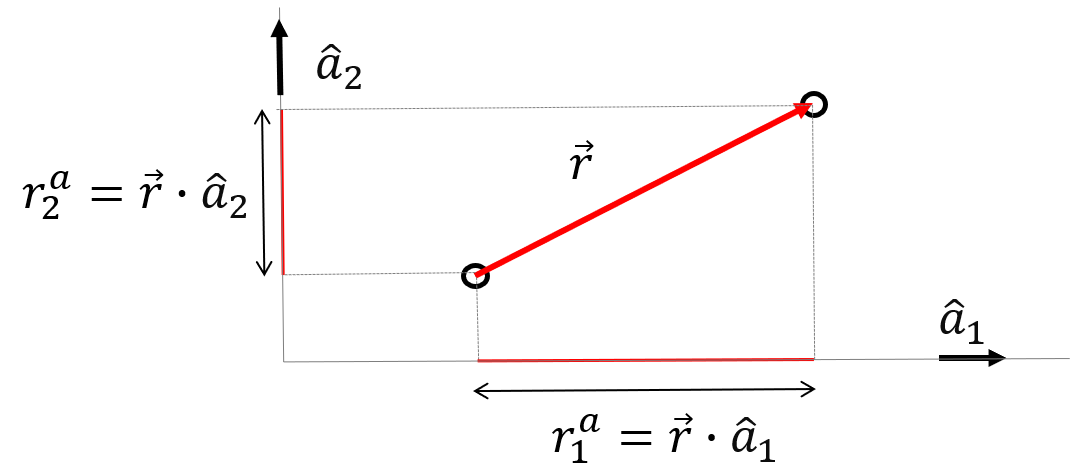
\includegraphics[width=0.50\textwidth]{vecpospro2.png}
				\label{fig:vecpospro2}}
				\hspace{+20pt}
				\subfloat[Décomposition selon les directions de la base]{
				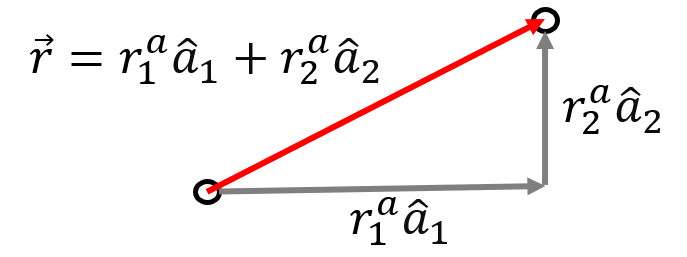
\includegraphics[width=0.40\textwidth]{vecpospro3.png}
				\label{fig:vecpospro3}}
				%\vspace{+30pt}
        \caption{Relations entre le vecteur géométrique de position et les composantes du vecteur-colonne}
				\label{fig:vecpospro23}
\end{figure}
%%%%%%%%%%%%%%%%%%%%%%%%%%%%%%%%%%%%%%%%%%%%%%%%%%%%%%%%%%%%%%%%%


%%%%%%%%%%%%%%%%%%%%%%%%%%%%%%%%%%%%%%%%%%%%%%%%%%%
\subsection{Transfert d'une équation vectorielle vers une équation matricielle} 
%
Lorsque les composantes de plusieurs vecteurs sont exprimées avec la même base, il est possible de faire des opérations directement avec les vecteur-colonnes de composantes. Cela permet de traiter simultanément les calculs de plusieurs axes, et aussi de faire des calculs numériques efficaces en utilisant les outils de l'algèbre linéaire. Par exemple, les additions et soustractions de vecteurs géométriques peuvent être calculées directement en termes des vecteur-colonnes dans une base:
%%%%%%%%%%%%%%%%%%%%%%%%%%%%%%%%%%%
\begin{equation}
\vec{u}   = \vec{v} + \vec{w}   \quad \Rightarrow \quad
\col{u}^a = \col{v}^a + \col{w}^a
\end{equation} 
%%%%%%%%%%%%%%%%%%%%%%%%%%%%%%%%%%%
Ce transfert d'une seule équation vectorielle à une équation matricielle (équivalent à un système de trois équations scalaires) correspond à une projection de l'équation vectorielle sur chacun des axes de la base:
%%%%%%%%%%%%%%%%%%%%%%%%%%%%%%%%%%%
\begin{equation}
\vec{u}   = \vec{v} + \vec{w}   
\quad \Rightarrow \quad
\left[ \begin{array}{c} (\vec{u}   = \vec{v} + \vec{w}  ) \bullet \hat{a}_1 \\ (\vec{u}   = \vec{v} + \vec{w}  ) \bullet \hat{a}_2 \\ (\vec{u}   = \vec{v} + \vec{w}  ) \bullet \hat{a}_3  \end{array} \right] 
\quad \Rightarrow \quad
\left[ \begin{array}{c}  u_1^a   = v_1^a + w_1^a   \\  u_2^a   = v_2^a + w_2^a   \\ u_3^a   = v_3^a + w_3^a   \end{array} \right] 
\quad \Rightarrow \quad
\col{u}^a = \col{v}^a + \col{w}^a
\end{equation} 
%%%%%%%%%%%%%%%%%%%%%%%%%%%%%%%%%%%

Les équations vectorielles avec des vecteurs de position peuvent donc être substituées par des équations matricielles équivalentes avec les vecteur-colonnes,\textbf{ à condition que tous les vecteur-colonnes soient exprimés dans une base commune}. 

%Voici quelques exemples de substitution d'équation de vecteurs de position vers des équations matricielles:
%%%%%%%%%%%%%%%%%%%%%%%%%%%%%%%%%%%%
%\begin{align}
%\vec{r}_{B/C}   = \vec{r}_{B/A} - \vec{r}_{C/A}   
%\quad &\Rightarrow \quad  \col{r}_{B/C}^a   = \col{r}_{B/A}^a - \col{r}_{C/A}^a 
%\\
%\vec{r}_{B/C}   = \vec{r}_{B/A} - \vec{r}_{C/A} \quad &\Rightarrow \quad \col{r}_{B/C}^b   = \col{r}_{B/A}^b - \col{r}_{C/A}^b 
%\\
%2  \vec{r}_{D/A} = 3 \vec{r}_{B/A} + \vec{r}_{C/A} \quad &\Rightarrow \quad  2  \col{r}_{D/A}^a = 3 \col{r}_{B/A}^a + \col{r}_{C/A}^a
%\end{align} 
%%%%%%%%%%%%%%%%%%%%%%%%%%%%%%%%%%%%
\textbf{Note:} Lors de l'écriture d'un programme informatique pour effectuer des calculs de cinématique, les calculs numériques doivent être fait en termes de composantes. En effet, les ordinateurs sont adaptés à manipuler des chiffres, des vecteur-colonnes de chiffres, des matrices de chiffres, etc. Toutefois, un ordinateur ne peut manipuler directement des éléments conceptuels comme les vecteurs unitaires.  

%%%%%%%%%%%%%%%%%%%%%%%%%%%%%%%%%%%%%%%%%%%%%%%%%%%
\subsection{Opérations avec les vecteur-colonnes} 
%
Les opérations vectorielles ont des équivalents en termes d'opérations matricielle avec les vecteur-colonnes qui sont très utiles pour les calculs numériques. Cette section introduit les opérations principales utiles pour la cinématique.

\subsubsection{Produit scalaire}
Un produit scalaire peut être calculé directement par une opération matricielle avec les vecteur-colonnes appelée produit intérieur (\textit{inner product}):
%%%%%%%%%%%%%%%%%%%%%%%%%%%%%%%%%%%
\begin{equation}
\vec{u} \bullet \vec{v} = \col{u}^T \col{v} = \left[ \begin{array}{c c c} u_1 & u_2 & u_3  \end{array} \right]  \left[ \begin{array}{c} v_1 \\ v_2 \\ v_3  \end{array} \right]
= u_1 v_1 + u_2 v_2 + u_3 v_3
\end{equation} 
%%%%%%%%%%%%%%%%%%%%%%%%%%%%%%%%%%%
si $\col{u}$ et $\col{v}$ sont les composantes exprimées dans une base vectorielle commune, par exemple:
%%%%%%%%%%%%%%%%%%%%%%%%%%%%%%%%%%%
\begin{align}
\vec{u} \bullet \vec{v} &= (\col{u}^a)^T \col{v}^a = (\col{u}^b)^T \col{v}^b
\end{align} 
%%%%%%%%%%%%%%%%%%%%%%%%%%%%%%%%%%%
mais attention car: 
%%%%%%%%%%%%%%%%%%%%%%%%%%%%%%%%%%%
\begin{align}
\vec{u} \bullet \vec{v} &\ne (\col{u}^a)^T \col{v}^b \\
\vec{u} \bullet \vec{v} &\ne (\col{u}^b)^T \col{v}^a 
\end{align} 
%%%%%%%%%%%%%%%%%%%%%%%%%%%%%%%%%%%
Il est à noter que l'ordre de multiplication ne change pas le résultat pour le produit scalaire:
%%%%%%%%%%%%%%%%%%%%%%%%%%%%%%%%%%%
\begin{equation}
\vec{u} \bullet \vec{v} = \vec{v} \bullet \vec{u} = \col{u}^T \col{v} = \col{v}^T \col{u} 
\end{equation} 
%%%%%%%%%%%%%%%%%%%%%%%%%%%%%%%%%%%

\paragraph{Normes, projections et calcul d'angles:}
Lorsqu'on connait les composantes de vecteurs dans une base commune, le produit intérieur peut être utilisé pour calculer la longueur d'un vecteur position:
%%%%%%%%%%%%%%%%%%%%%%%%%%%%%%%%%%%
\begin{align}
\|\vec{r}\|^2 &= \vec{r} \bullet \vec{r} = \col{r}^T \col{r} = r_1^2 + r_2^2 + r_3^2
\end{align} 
%%%%%%%%%%%%%%%%%%%%%%%%%%%%%%%%%%%
pour calculer une distance projetée selon un axe décrit par un vecteur unitaire $\hat{n}$:
%%%%%%%%%%%%%%%%%%%%%%%%%%%%%%%%%%%
\begin{align}
d_n &= \vec{r} \bullet \hat{n} = \col{r}^T \col{n} = r_1 n_1 + r_2 n_2 + r_3 n_3
\end{align} 
%%%%%%%%%%%%%%%%%%%%%%%%%%%%%%%%%%%
et pour calculer un angle entre deux vecteurs unitaires $\hat{x}$ et $\hat{y}$:
%%%%%%%%%%%%%%%%%%%%%%%%%%%%%%%%%%%
\begin{align}
\cos \angle (\hat{x},\hat{y}) = \hat{x} \bullet \hat{y} = \col{x}^T \col{y} = x_1 y_1 + x_2 y_2 + x_3 y_3
\end{align} 
%%%%%%%%%%%%%%%%%%%%%%%%%%%%%%%%%%%

%%%%%%%%%%%%%%%%%%%%%%%%%%%%%%%%%%%
\subsubsection{Produit vectoriel}
%
Un produit vectoriel (\textit{cross product}) peut être calculé directement par une opération matricielle définie avec les vecteur-colonnes:
%%%%%%%%%%%%%%%%%%%%%%%%%%%%%%%%%%%
\begin{equation}
\vec{u} = \vec{v} \times \vec{w} \quad \Rightarrow \quad  \col{u} = \col{v}^{\times}\col{w} \quad \Rightarrow \quad 
 \left[ \begin{array}{c} u_1 \\ u_2 \\ u_3  \end{array} \right] = 
\left[ \begin{array}{c c c}
	0 & -v_3 & v_2  \\ v_3 & 0 & -v_1 \\ -v_2 & v_1 & 0
\end{array}  \right]
 \left[ \begin{array}{c} w_1 \\ w_2 \\ w_3  \end{array} \right]
\end{equation} 
%%%%%%%%%%%%%%%%%%%%%%%%%%%%%%%%%%%
L'ordre de multiplication est important pour le produit vectoriel, il change la direction du vecteur résultant:
%%%%%%%%%%%%%%%%%%%%%%%%%%%%%%%%%%%
\begin{equation}
\vec{u} = \vec{v} \times \vec{w} =  -\vec{w} \times \vec{v} \quad \Rightarrow \quad  \col{u} = \col{v}^{\times}\col{w} = - \col{w}^{\times}\col{v}
\end{equation} 
%%%%%%%%%%%%%%%%%%%%%%%%%%%%%%%%%%%

\paragraph{Vecteurs unitaires d'une base vectorielle:}
Il est possible de calculer les composantes d'un vecteur unitaire qui complète une base vectorielle avec une opération de produit vectorielle, connaissant les composantes de deux vecteurs unitaires orthogonaux: 
%%%%%%%%%%%%%%%%%%%%%%%%%%%%%%%%%%%
\begin{equation}
\hat{b}_3 = \hat{b}_1 \times \hat{b}_2  \quad \Rightarrow \quad   \col{b}_3 = \col{b}_1^{\times}\col{b}_2
\end{equation} 
%%%%%%%%%%%%%%%%%%%%%%%%%%%%%%%%%%%

\paragraph{Note:}
Pour alléger la présentation, les exposants qui spécifient les bases vectorielles associées aux vecteur-colonnes sont parfois omis dans les équations, on considère alors que tous les vecteur-colonnes impliqués dans l'équation sont exprimés dans une base vectorielle commune.


%%%%%%%%%%%%%%%%%%%%%%%%%%%%%%%%%%%
\subsubsection{Changement de base}
%
Les composantes d'un vecteur géométrique $\vec{v}$ dans une base $a$ peuvent être directement reliées aux composantes du même vecteur géométrique $\vec{v}$ dans une autre base $b$, par une équation matricielle qui implique les vecteur-colonnes et une matrice 3$\times$3 appelée une \textit{matrice de rotation}. On va noter une matrice $^bR^a$ lorsqu'une multiplication par la gauche de cette matrice avec un vecteur colonne $\col{v}^a$ donne le vecteur-colonne $\col{v}^b$:
%%%%%%%%%%%%%%%%
\begin{align}
\col{v}^b &= {}^bR^a \col{v}^a  \quad \Rightarrow \quad
 \left[ \begin{array}{c} v_1^b \\ v_2^b \\ v_3^b  \end{array} \right]
=
\left[ \begin{array}{c c c}
	{}^bR^a_{11} & {}^bR^a_{12} & {}^bR^a_{13} \\ 
	{}^bR^a_{21} & {}^bR^a_{22} & {}^bR^a_{23} \\
	{}^bR^a_{31} & {}^bR^a_{32} & {}^bR^a_{33}
\end{array}  \right]
 \left[ \begin{array}{c} v_1^a \\ v_2^a \\ v_3^a  \end{array} \right]
\label{eq:basechange1}
\end{align} 
%%%%%%%%%%%%%%%%%
Les propriétés et le calcul des matrices de rotation seront traités en détails à la section \ref{sec:changematrice}.



%%%%%%%%%%%%%%%%%%%%%%%%%%%%%%%%%%%%%%%%%%%%%%%%%%%%
%\subsection{Calculs appliqués dans un contexte de cinématique} 
%%
%\paragraph{Normes, projections et calcul d'angles:}
%Lorsque qu'on connait les composantes de vecteurs dans une base commune, le produit intérieur peut être utilisé pour calculer la longueur d'un vecteur position:
%%%%%%%%%%%%%%%%%%%%%%%%%%%%%%%%%%%%
%\begin{align}
%\|\vec{r}\|^2 &= \vec{r} \bullet \vec{r} = \col{r}^T \col{r} = r_1^2 + r_2^2 + r_3^2
%\end{align} 
%%%%%%%%%%%%%%%%%%%%%%%%%%%%%%%%%%%%
%pour calculer une distance projeté selon un axe décrit par un vecteur unitaire $\hat{n}$:
%%%%%%%%%%%%%%%%%%%%%%%%%%%%%%%%%%%%
%\begin{align}
%d_n &= \vec{r} \bullet \hat{n} = \col{r}^T \col{n} = r_1 n_1 + r_2 n_2 + r_3 n_3
%\end{align} 
%%%%%%%%%%%%%%%%%%%%%%%%%%%%%%%%%%%%
%et pour calculer un angle entre deux vecteurs unitaires $\hat{x}$ et $\hat{y}$:
%%%%%%%%%%%%%%%%%%%%%%%%%%%%%%%%%%%%
%\begin{align}
%\cos \angle (\hat{x},\hat{y}) = \hat{x} \bullet \hat{y} = \col{x}^T \col{y} = x_1 y_1 + x_2 y_2 + x_3 y_3
%\end{align} 
%%%%%%%%%%%%%%%%%%%%%%%%%%%%%%%%%%%%
%
%\paragraph{Vecteurs unitaires:}
%Il est possible de calculer les composantes d'un vecteur unitaire qui complète une base vectorielle avec une opération de produit vectorielle, connaissant les composantes de deux vecteurs unitaires orthogonaux: 
%%%%%%%%%%%%%%%%%%%%%%%%%%%%%%%%%%%%
%\begin{equation}
%\hat{b}_3 = \hat{b}_1 \times \hat{b}_2  \quad \Rightarrow \quad   \col{b}_3 = \col{b}_1^{\times}\col{b}_2
%\end{equation} 
%%%%%%%%%%%%%%%%%%%%%%%%%%%%%%%%%%%%


%%%%%%%%%%%%%%%%%%%%%%%%%%%%%%%%%%%%%%%%%%%%%%%%%%%
\subsection{Invariants} 
%
Le vecteur géométrique $\vec{r}$ est une quantité constante peu importe la base vectorielle utilisée: 
%%%%%%%%%%%%%%%
\begin{equation}
\vec{r} = \sum_{i} r_i^a \hat{a}_i = \sum_{i} r_i^b \hat{b}_i = \sum_{i} r_i^c \hat{c}_i
\end{equation}
%%%%%%%%%%%%%%%
mais le vecteur-colonne dépend de la base vectorielle. Les vecteur-colonnes sont en générale différents sauf dans le cas particulier de bases vectorielles coïncidentes:
%%%%%%%%%%%%%%%%%%%%%%%%%%%%%%%%%%%
\begin{equation}
\col{r}^{a} \ne \col{r}^{b} \quad\quad \text{sauf dans le cas particulier:} \quad \hat{a}_1 = \hat{b}_1 \;,\; \hat{a}_2 = \hat{b}_2  \;\text{et}\; \hat{a}_3 = \hat{b}_3 
\end{equation} 
%%%%%%%%%%%%%%%%%%%%%%%%%%%%%%%%%%%
La longueur du vecteur géométrique étant une constante peut importe la base vectorielle utilisée, il est possible d'établir la relation suivante entre les vecteur-colonnes utilisant différentes bases:
%%%%%%%%%%%%%%%
\begin{equation}
\|\vec{r}\|^2 = \vec{r} \bullet \vec{r} = (\col{r}^{a})^T \col{r}^{a} = (\col{r}^{b})^T \col{r}^{b} = (\col{r}^{c})^T \col{r}^{c}
\end{equation}
%%%%%%%%%%%%%%%
La norme des vecteur-colonnes est donc invariante par rapport au choix de la base. 





%%%%%%%%%%%%%%%%%%%%%%%%%%%%%%%%%%%%%%%%%%%%%%%%%%
\subsection{Exemple: calcul de la position globale de l'effecteur d'un robot}
\label{sec:exer-cinematique-base}
%
Dans cet exemple, le robot précédemment étudié (Figure \ref{fig:vecposunipro}) est ici analysé à nouveau mais cette fois avec l'aide des bases vectorielles. L'objectif est ici de calculer la position du point $D$ par rapport au point $A$ exprimée dans la base vectorielle $a$. Comme illustré à la figure \ref{fig:vecposbase1}, la première étape est de décrire la position qui doit être calculée en terme de vecteurs de position géométriques:
%%%%%%%%%%%%%%%%%%%%%%%%%%%%%%%%%%%
\begin{align}
\vec{r}_{D/A} &= \vec{r}_{D/C} + \vec{r}_{C/B} + \vec{r}_{B/A}
\end{align} 
%%%%%%%%%%%%%%%%%%%%%%%%%%%%%%%%%%%
Cette relation vectorielle peut ensuite être convertie en une équation matricielle entre les composantes dans une base $a$ fixe qui correspond aux axes selon lesquels la position doit être exprimée:
%%%%%%%%%%%%%%%%%%%%%%%%%%%%%%%%%%%
\begin{align}
\col{r}_{D/A}^a &= \col{r}_{D/C}^a + \col{r}_{C/B}^a + \col{r}_{B/A}^a
\label{eq:exaddbase}
\end{align} 
%%%%%%%%%%%%%%%%%%%%%%%%%%%%%%%%%%%
Ensuite, comme illustré à la Figure \ref{fig:vecposbase2}, les différents vecteurs positions qui représentent chaque joint ont des composantes connues dans des bases vectorielles locales attachées aux différents liens rigides du robot:
%%%%%%%%%%%%%%%%%%%%%%%%%%%%%%%%%%%
\begin{align}
\col{r}_{B/A}^b = 
\left[ \begin{array}{c} 
l_1 \\ 0 \\ 0
\end{array} \right] 
\quad\quad
\col{r}_{C/B}^c = 
\left[ \begin{array}{c} 
0 \\ l_2 \\ 0
\end{array} \right]
\quad\quad
\col{r}_{D/C}^d = 
\left[ \begin{array}{c} 
0 \\ l_3 \\ 0
\end{array} \right] 
\end{align} 
%%%%%%%%%%%%%%%%%%%%%%%%%%%%%%%%%%%
Il est à noter que ces vecteur-colonnes qui utilisent les bases locales sont constants et indépendants des angles des joints car les base locales tournent avec les liens rigides. Il est ensuite possible de convertir ces vecteur-colonnes de positions dans la base $a$ par des opérations de changement de base avec les matrices de rotation appropriées:
%%%%%%%%%%%%%%%%%%%%%%%%%%%%%%%%%%%
\begin{align}
\col{r}_{D/C}^a = {}^aR^d \, \col{r}_{D/C}^d 
\quad \quad
\col{r}_{C/B}^a = {}^aR^c \, \col{r}_{C/B}^c
\quad \quad
\col{r}_{B/A}^a = {}^aR^b \, \col{r}_{B/A}^b
\end{align} 
%%%%%%%%%%%%%%%%%%%%%%%%%%%%%%%%%%%
Finalement, en substituant dans l'équation \eqref{eq:exaddbase}, l'équation matricielle nécessaire pour obtenir les composantes du vecteur position $\vec{r}_{D/A}$ exprimé avec la base $a$ est obtenue:
%%%%%%%%%%%%%%%%%%%%%%%%%%%%%%%%%%%
\begin{align}
\col{r}_{D/A}^a &= {}^aR^d \, \col{r}_{D/C}^d + {}^aR^c \, \col{r}_{C/B}^c + {}^aR^b \, \col{r}_{B/A}^b
\label{eq:ex333cinematique}
\end{align} 
%%%%%%%%%%%%%%%%%%%%%%%%%%%%%%%%%%%
Les matrices de rotation doivent ensuite être calculées pour solutionner cette équation, voir section \ref{sec:exer-cinematique-base2} pour la suite de cet exemple. 
%%%%%%%%%%%%%%%%%%%%%%%%%%%%%%%%%%%%%%%%%%%%%%%%%%%%%%%%%%%%%%%
\begin{figure}[htb]
				%\vspace{-10pt}
        \centering
				\subfloat[Construction géométrique]{
				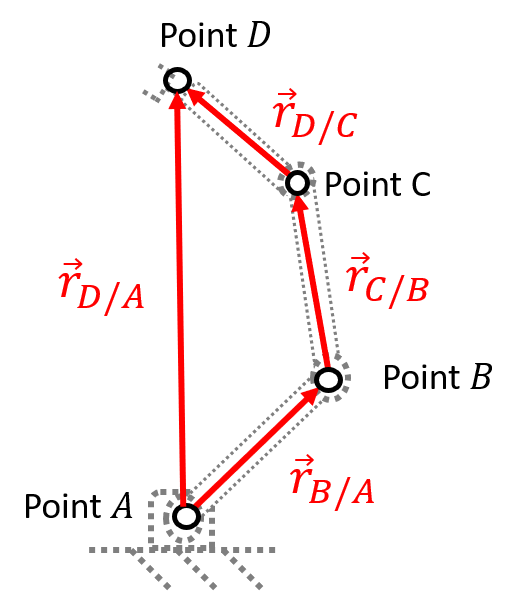
\includegraphics[width=0.30\textwidth]{vecposcons}
				\label{fig:vecposbase1}}
				%%%%
				\hspace{10pt}
				%%%%
        \subfloat[Bases vectorielles]{
				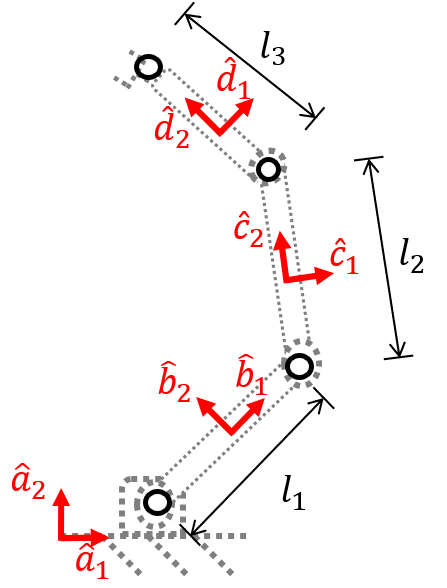
\includegraphics[width=0.27\textwidth]{vecposbase}
				\label{fig:vecposbase2}}
				%%%%
				%\hspace{10pt}
				%%%%
        %\subfloat[Angles]{
				%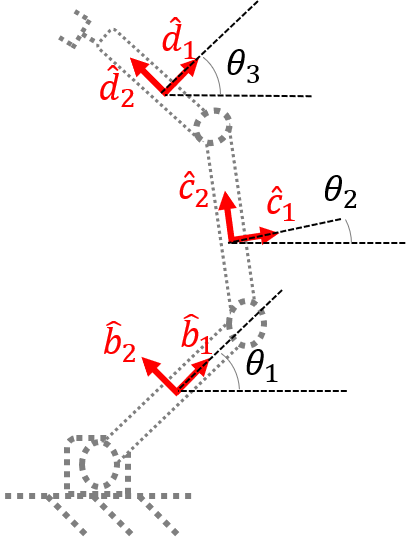
\includegraphics[width=0.27\textwidth]{vecposbaseangle}
				%\label{fig:vecposbaseangle}}
        \caption{Exemple d'un calcul de la position de l'effecteur d'un robot avec une utilisation des bases vectorielles}
				\label{fig:vecposbase}
\end{figure}
%%%%%%%%%%%%%%%%%%%%%%%%%%%%%%%%%%%%%%%%%%%%%%%%%%%%%%%%%%%%%%%%%


%%%%%%%%%%%%%%%%%%%%%%%%%%%%%%%%%%%
\subsection{Exemple: distance projetée calculée avec les vecteur-colonnes}
%
Comme illustré à la figure \ref{fig:exprojcomp}, cet exemple démontre comment calculer la distance projetée $d_n$ d'un vecteur $\vec{r}_{C/A}$ selon un axe décrit par $\hat{n}$, connaissant les vecteur-colonnes de composantes:
%%%%%%%%%%%%%%%%%%%%%%%%%%%%%%%%%%%
\begin{align}
\col{r}_{C/B}^b = \left[ \begin{array}{c} x \\ y \\ z  \end{array} \right]
\quad\quad
\col{r}_{B/A}^a = \left[ \begin{array}{c} X \\ Y \\ Z  \end{array} \right]
\quad\quad
\col{n}^b       = \left[ \begin{array}{c} n_x \\ n_y \\ n_z  \end{array} \right]
\label{eq:disprojexdef}
\end{align} 
%%%%%%%%%%%%%%%%%%%%%%%%%%%%%%%%%%%
Premièrement, l'équation vectorielle de vecteurs géométriques de position est développée:
%%%%%%%%%%%%%%%%%%%%%%%%%%%%%%%%%%%
\begin{align}
\vec{r}_{C/A} = \vec{r}_{C/B} + \vec{r}_{B/A}
\end{align} 
%%%%%%%%%%%%%%%%%%%%%%%%%%%%%%%%%%%
pour ensuite effectuer le produit scalaire pour calculer la distance projetée:
%%%%%%%%%%%%%%%%%%%%%%%%%%%%%%%%%%%
\begin{align}
d_n = \vec{r}_{C/A} \bullet \hat{n} = (\vec{r}_{C/B} + \vec{r}_{B/A} ) \bullet \hat{n} 
\end{align} 
%%%%%%%%%%%%%%%%%%%%%%%%%%%%%%%%%%%
Deuxièmement, on choisi la base $b$ pour transformer la relation vectorielle en équation matricielle:
%%%%%%%%%%%%%%%%%%%%%%%%%%%%%%%%%%%
\begin{align}
d_n &= (\col{r}_{C/B}^b + \col{r}_{B/A}^b )^T \col{n}^b \\
d_n &= ( \col{r}_{C/B}^b )^T \col{n}^b + ( \col{r}_{B/A}^b )^T \col{n}^b
\end{align} 
%%%%%%%%%%%%%%%%%%%%%%%%%%%%%%%%%%%
Tous les vecteur-colonnes sont connus sauf le vecteur-colonne $\col{r}_{C/B}^b$, qui doit être substitué par $\col{r}_{C/B}^b = {}^bR^a \, \col{r}_{C/B}^a$ car les composantes de $\vec{r}_{C/B}$ sont connues seulement dans la base $a$. On obtient alors:
%%%%%%%%%%%%%%%%%%%%%%%%%%%%%%%%%%%
\begin{align}
d_n &= ( {}^bR^a \, \col{r}_{C/B}^a )^T \col{n}^b + ( \col{r}_{B/A}^b )^T \col{n}^b \\
d_n &= ( \col{n}^b )^T \, {}^bR^a \, \col{r}_{C/B}^a + ( \col{r}_{B/A}^b )^T \col{n}^b 
\end{align} 
%%%%%%%%%%%%%%%%%%%%%%%%%%%%%%%%%%%
et ce qui correspond en termes de composantes à l'équation:
%%%%%%%%%%%%%%%%%%%%%%%%%%%%%%%%%%%
\begin{align}
d_n &= \left[ \begin{array}{c c c}
	n_1^b & n_2^b & n_3^b  
\end{array}  \right]
\left[ \begin{array}{c c c}
	{}^bR^a_{11} & {}^bR^a_{12} & {}^bR^a_{13} \\ 
	{}^bR^a_{21} & {}^bR^a_{22} & {}^bR^a_{23} \\
	{}^bR^a_{31} & {}^bR^a_{32} & {}^bR^a_{33}
\end{array}  \right]
 \left[ \begin{array}{c} r_{C/B,1}^a \\ r_{C/B,2}^a \\ r_{C/B,3}^a  \end{array} \right]
+
\left[ \begin{array}{c c c}
	r_{B/A,1}^b & r_{B/A,2}^b & r_{B/A,3}^b  
\end{array}  \right]
 \left[ \begin{array}{c} n_1^b \\ n_2^b \\ n_3^b  \end{array} \right]
\end{align} 
%%%%%%%%%%%%%%%%%%%%%%%%%%%%%%%%%%%
si on substitue par les composantes connues définies à l'équation \eqref{eq:disprojexdef}:
%%%%%%%%%%%%%%%%%%%%%%%%%%%%%%%%%%%
\begin{align}
d_n &=
\left[ \begin{array}{c c c}
	n_x & n_y & n_z  
\end{array}  \right]
\left[ \begin{array}{c c c}
	{}^bR^a_{11} & {}^bR^a_{12} & {}^bR^a_{13} \\ 
	{}^bR^a_{21} & {}^bR^a_{22} & {}^bR^a_{23} \\
	{}^bR^a_{31} & {}^bR^a_{32} & {}^bR^a_{33}
\end{array}  \right]
 \left[ \begin{array}{c} x \\ y \\ z  \end{array} \right]
+
\left[ \begin{array}{c c c}
	X & Y & Z  
\end{array}  \right]
 \left[ \begin{array}{c} n_x \\ n_y \\ n_z  \end{array} \right]
\end{align} 
%%%%%%%%%%%%%%%%%%%%%%%%%%%%%%%%%%%
C'est donc cette équation qui devrait être programmée pour faire ce calcul numériquement sur un ordinateur.
%%%%%%%%%%%%%%%%%%%%%%%%%
\begin{figure}[htbp]
	\centering
		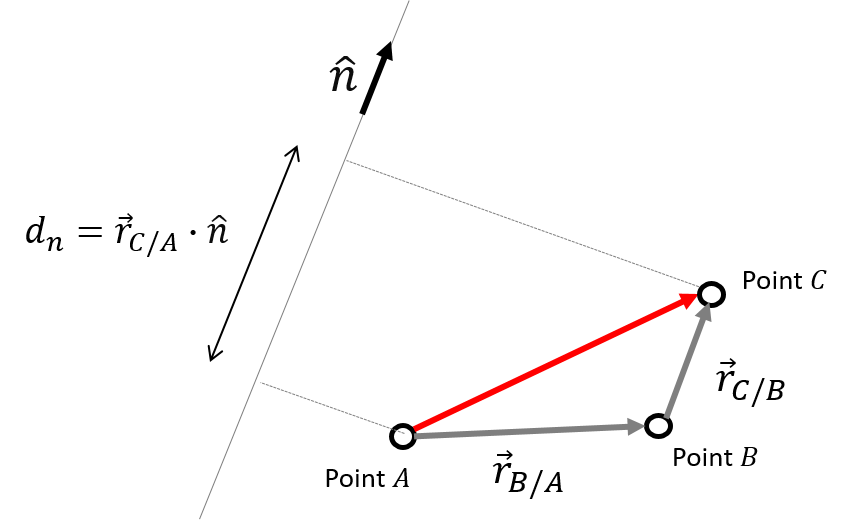
\includegraphics[width=0.50\textwidth]{exprojcomp.png}
	\caption{Exemple de calcul d'une distance projetée}
	\label{fig:exprojcomp}
\end{figure}
%%%%%%%%%%%%%%%%%%%%%%%%%%%



%%%%%%%%%%%%%%%%%%%%%%%%%%%%%%%%%%%%%%%%%%%%%%%%%%%%%%%%%%%%%%%%%%%%%%
\newpage
\section{Les matrices de rotations}
\label{sec:changematrice}

Une matrice de rotation notée $^bR^a$, est une matrice (3$\times$3 en 3D) qui permet de calculer directement les composants d'un vecteur position dans une base $b$ avec les composants connus dans une base $a$, i.e. effectuer un \textbf{changement de base}, par une multiplication de la forme:
%%%%%%%%%%%%%%%%
\begin{align}
\col{r}^b &= {}^bR^a \col{r}^a
\label{eq:basechange}
\end{align} 
%%%%%%%%%%%%%%%%%
La matrice de rotation est un raccourci pour projeter un vecteur position sur trois nouveaux axes en une seule opération matricielle, plutôt que d'effectuer trois opérations de projection indépendantes. 

\paragraph{Note:} Une matrice de rotation a deux fonctions majeures dans un contexte de cinématique: \textbf{1)} effectuer des opérations de changement de base et \textbf{2)} représenter une orientation relative. Cette section présente le rôle des matrices de rotation pour les opérations de changement de base, les matrices de rotation seront discutées à nouveau dans le contexte de la représentation de l'orientation d'un corps rigide à la section \ref{sec:corps}.


%%%%%%%%%%%%%%%%%%%%%%%%%%%%%%%%%%%%%%%
\subsection{Exemple: matrice de rotation dans le plan calculée par trigonométrie}

La figure \ref{fig:basechange2d} montre un exemple d'un vecteur $\vec{r}$ en 2 dimensions exprimé dans deux base vectorielles $b$ et $a$. Comme illustré à la figure \ref{fig:r_trigo}, avec une construction de triangles il est possible de déterminer par trigonométrie les relations entre les composantes dans les deux bases, et donc la matrice de rotation ${}^aR^b$. L'approche par trigonométrie est toutefois limitée pour les rotations en 3D, une approche vectorielle plus simple et plus universelle pour calculer des matrices de rotation est présentée à la section \ref{sec:calmat}.
%%%%%%%%%%%%%
\begin{figure}[htbp]
	\centering
		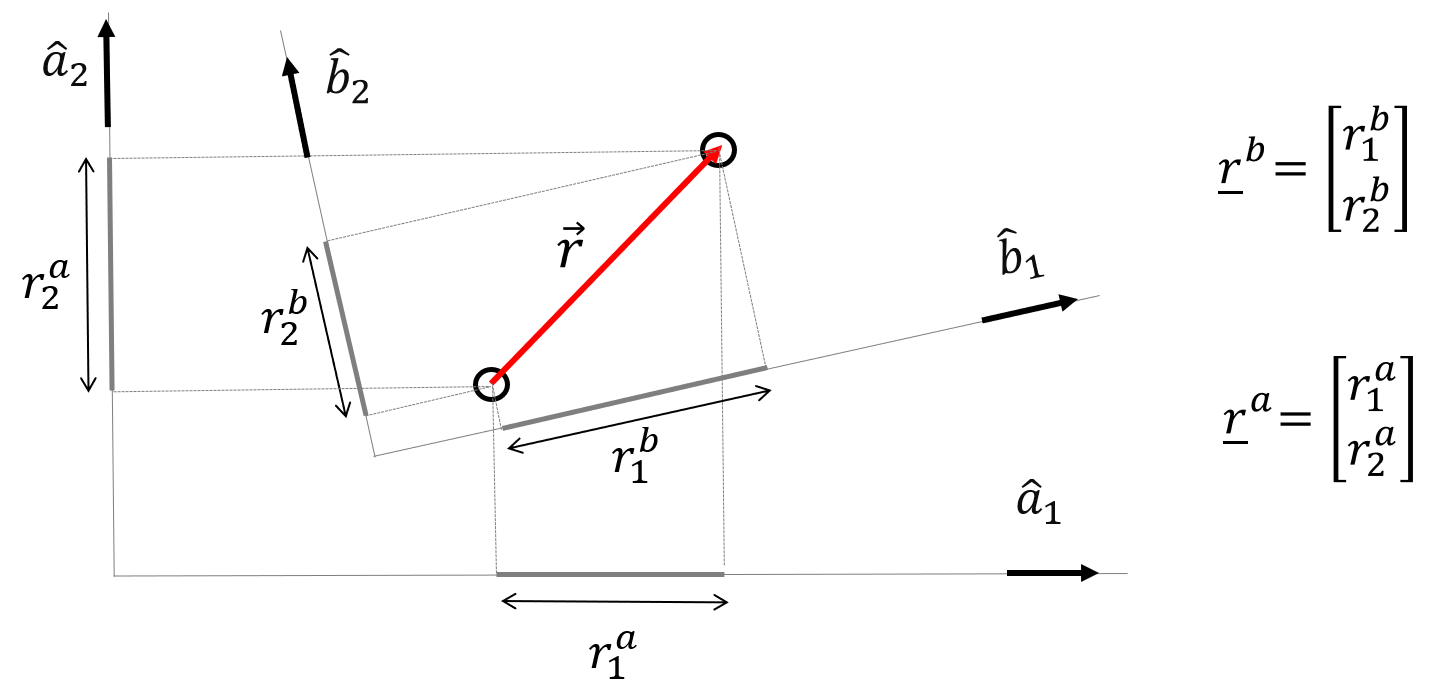
\includegraphics[width=0.65\textwidth]{basechange.png}
	\caption{Vecteur position exprimé dans deux bases vectorielles}
	\label{fig:basechange2d}
\end{figure}
%%%%%%%%%%%%%%
%%%%%%%%%%%%%
\begin{figure}[hb]
	\centering
		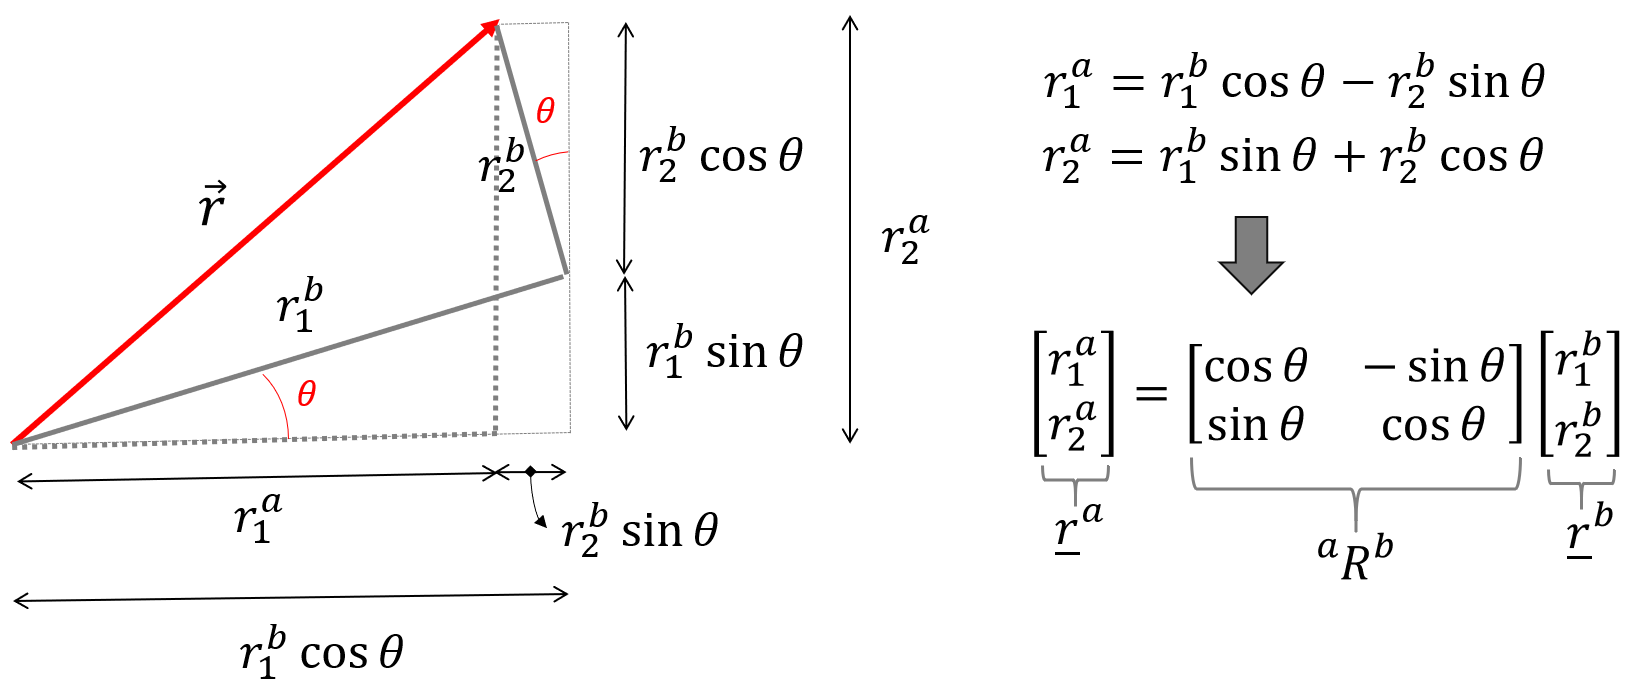
\includegraphics[width=0.65\textwidth]{r_trigo.png}
	\caption{Calcul par trigonométrie de la matrice de rotation 2x2 ${}^aR^b$ pour le changement de base illustré à la figure \ref{fig:basechange2d}}
	\label{fig:r_trigo}
\end{figure}
%%%%%%%%%%%%%%


%%%%%%%%%%%%%%%%%%%%%%%%%%%%%%%%%%%%%%%
\subsection{Origine de la matrice}
%Cette section démontre l'équation \eqref{eq:basechange} basé sur les définitions des vecteur-colonnes de composants. 
Si les composantes d'un vecteur $\vec{r}$ sont connus dans une base $a$:
%%%%%%%%%%%%%%%%%%%%%%%%%%%%%%%%%%%
\begin{align}
\col{r}^a &= \left[ \begin{array}{c} r_1^a \\ r_2^a \\ r_3^a  \end{array} \right]
\end{align} 
%%%%%%%%%%%%%%%%%%%%%%%%%%%%%%%%%%%
le vecteur géométrique associé est donné par:
%%%%%%%%%%%%%%%%%%%%%%%%%%%%%%%%%%%
\begin{align}
\vec{r} &= r_1^a \hat{a}_1 + r_2^a \hat{a}_2 + r_3^a \hat{a}_3
\label{eq:pvec}
\end{align} 
%%%%%%%%%%%%%%%%%%%%%%%%%%%%%%%%%%%
Les composantes dans une base $b$ peuvent être calculées par des produits scalaires suivants:
%%%%%%%%%%%%%%%%%%%%%%%%%%%%%%%%%%%
\begin{align}
r_1^b &= \vec{r} \bullet \hat{b}_1 \\
r_2^b &= \vec{r} \bullet \hat{b}_2 \\
r_3^b &= \vec{r} \bullet \hat{b}_3
\end{align} 
%%%%%%%%%%%%%%%%%%%%%%%%%%%%%%%%%%%
Si on substitue $\vec{r}$ par l'équation \eqref{eq:pvec}:
%%%%%%%%%%%%%%%%%%%%%%%%%%%%%%%%%%%
\begin{align}
r_1^b &= (r_1^a \hat{a}_1 + r_2^a \hat{a}_2 + r_3^a \hat{a}_3) \bullet \hat{b}_1 \\
r_2^b &= (r_1^a \hat{a}_1 + r_2^a \hat{a}_2 + r_3^a \hat{a}_3) \bullet \hat{b}_2 \\
r_3^b &= (r_1^a \hat{a}_1 + r_2^a \hat{a}_2 + r_3^a \hat{a}_3) \bullet \hat{b}_3
\end{align} 
%%%%%%%%%%%%%%%%%%%%%%%%%%%%%%%%%%%
et on réarrange les termes:
%%%%%%%%%%%%%%%%%%%%%%%%%%%%%%%%%%%
\begin{align}
r_1^b &= (\hat{a}_1 \bullet \hat{b}_1 ) r_1^a + (\hat{a}_2 \bullet \hat{b}_1 ) r_2^a + (\hat{a}_3 \bullet \hat{b}_1 ) r_3^a \\
r_2^b &= (\hat{a}_1 \bullet \hat{b}_2 ) r_1^a + (\hat{a}_2 \bullet \hat{b}_2 ) r_2^a + (\hat{a}_3 \bullet \hat{b}_2 ) r_3^a \\
r_3^b &= (\hat{a}_1 \bullet \hat{b}_3 ) r_1^a + (\hat{a}_2 \bullet \hat{b}_3 ) r_2^a + (\hat{a}_3 \bullet \hat{b}_3 ) r_3^a 
\end{align} 
%%%%%%%%%%%%%%%%%%%%%%%%%%%%%%%%%%%
On obtient trois équations qui peuvent être regroupées sous forme matricielle:
%%%%%%%%%%%%%%%%%%%%%%%%%%%%%%%%%%%
\begin{align}
\underbrace{ \left[ \begin{array}{c} r_1^b \\ r_2^b \\ r_3^b  \end{array} \right] }_{\col{r}^b}
=
\underbrace{ \left[ \begin{array}{c c c} 
\hat{a}_1 \bullet \hat{b}_1 & \hat{a}_2 \bullet \hat{b}_1 & \hat{a}_3 \bullet \hat{b}_1 \\
\hat{a}_1 \bullet \hat{b}_2 & \hat{a}_2 \bullet \hat{b}_2 & \hat{a}_3 \bullet \hat{b}_2 \\
\hat{a}_1 \bullet \hat{b}_3 & \hat{a}_2 \bullet \hat{b}_3 & \hat{a}_3 \bullet \hat{b}_3 
\end{array} \right] }_{^bR^a}
\underbrace{ \left[ \begin{array}{c} r_1^a \\ r_2^a \\ r_3^a  \end{array} \right] }_{\col{r}^a}
\label{eq:Rdot}
\end{align} 
%%%%%%%%%%%%%%%%%%%%%%%%%%%%%%%%%%%

La matrice de rotation $^bR^a$ consiste donc à des produits scalaires entre les vecteurs unitaires des bases vectorielles $a$ et $b$. \textbf{L'opération de multiplication d'un vecteur-colonne $\col{r}^a$ par la matrice de rotation $^bR^a$ correspond à la projection du vecteur géométrique associé $\vec{r}$ sur la base vectorielle $b$.}



%%%%%%%%%%%%%%%%%%%%%%%%%%%%%%%%%%%%%%%%%%%%%%%%%%%%%%%%%%%%%
\subsection{Définitions}

Une matrice de rotation est définie par les produits scalaires des vecteurs unitaires qui forment deux bases vectorielles:
%%%%%%%%%%%%%%%%%%%%%%%%%%%%%%%%%%%
\begin{align}
{}^aR^b &= 
\left[ \begin{array}{c c c} 
\hat{a}_1 \bullet \hat{b}_1  &  \hat{a}_1 \bullet \hat{b}_2  &  \hat{a}_1 \bullet \hat{b}_3 \\
\hat{a}_2 \bullet \hat{b}_1  &  \hat{a}_2 \bullet \hat{b}_2  &  \hat{a}_2 \bullet \hat{b}_3 \\
\hat{a}_3 \bullet \hat{b}_1  &  \hat{a}_3 \bullet \hat{b}_2  &  \hat{a}_3 \bullet \hat{b}_3 
\end{array} \right] 
= 
\left[ \begin{array}{c c c} 
\cos \angle (\hat{a}_1 , \hat{b}_1)  &  \cos \angle (\hat{a}_1 , \hat{b}_2)  &  \cos \angle (\hat{a}_1 , \hat{b}_3) \\
\cos \angle (\hat{a}_2 , \hat{b}_1)  &  \cos \angle (\hat{a}_2 , \hat{b}_2)  &  \cos \angle (\hat{a}_2 , \hat{b}_3) \\
\cos \angle (\hat{a}_3 , \hat{b}_1)  &  \cos \angle (\hat{a}_3 , \hat{b}_2)  &  \cos \angle (\hat{a}_3 , \hat{b}_3) 
\end{array} \right]
\label{eq:cosinusdirecteurs}
\end{align} 
%%%%%%%%%%%%%%%%%%%%%%%%%%%%%%%%%%%
Les produits scalaires correspondent aussi aux cosinus des angles entre les vecteurs unitaires, c'est pourquoi la matrice de rotation est aussi parfois appelée la \textbf{matrice des cosinus directeurs}. Par inspection de l'équation \eqref{eq:cosinusdirecteurs}, on remarque que les colonnes de la matrice ${}^aR^b$ correspondent aux vecteur-colonnes des composantes des vecteurs unitaires $\hat{b}_i$ exprimées dans la base $a$ et que les rangés de la matrice ${}^aR^b$ correspondent à la transposée des vecteur-colonnes des composantes des vecteurs unitaires $\hat{a}_i$ exprimées dans la base $b$. Cela permet donc des définitions équivalentes plus compactes:
%%%%%%%%%%%%%%%%%%%%%%%%%%%%%%%%%%%
\begin{align}
{}^aR^b &= 
%\left[ \begin{array}{c c c} 
%\col{b}_1^a &  \col{b}_2^a & \col{b}_3^a
%\end{array} \right] 
%=
%\left[ \begin{array}{c} 
%(\col{a}_1^b)^T \\
%(\col{a}_2^b)^T \\
%(\col{a}_3^b)^T
%\end{array} \right] = 
\left[ \begin{array}{c c c} 
	\left[ \begin{array}{c} \\ \col{b}_1^a \\  \\ \end{array}  \right] & \left[ \begin{array}{c} \\ \col{b}_2^a \\  \\ \end{array}  \right] & \left[ \begin{array}{c} \\ \col{b}_3^a \\  \\ \end{array}  \right]
\end{array} \right]
=
\left[ \begin{array}{c} 
\left[ \begin{array}{c c c} & (\col{a}_1^b)^T & \end{array} \right] \\[\medskipamount]
\left[ \begin{array}{c c c} & (\col{a}_2^b)^T & \end{array} \right] \\[\medskipamount]
\left[ \begin{array}{c c c} & (\col{a}_3^b)^T & \end{array} \right] 
\end{array} \right] 
\label{eq:matricerotcol}
\end{align} 
%%%%%%%%%%%%%%%%%%%%%%%%%%%%%%%%%%%
Finalement, la matrice de rotation peut aussi être définie en termes de composantes et d'indices par:
%%%%%%%%%%%%%%%%%%%%%%%%%%%%%%%%%%%
\begin{align}
{}^aR^b_{ij} &= \hat{a}_i \bullet \hat{b}_j
\end{align} 
%%%%%%%%%%%%%%%%%%%%%%%%%%%%%%%%%%%
une équation qui est simple à se rappeler et permet d'éviter de mélanger l'ordre de rotation ${}^aR^b$ vs. ${}^bR^a$ avec la notation utilisée dans ces notes.

%%%%%%%%%%%%%%%%%%%%%%%%%%%%%%%%%%%
\subsection{Calcul des matrices de rotation basé sur les colonnes}
\label{sec:calmat}

La définition des matrices de rotation basée sur les vecteurs unitaires de eq.\eqref{eq:matricerotcol} est particulièrement utile pour calculer une matrice de rotation. Une astuce pour ne pas mélanger l'ordre de rotation ($^bR^a$ vs. $^aR^b$) est d'avoir en tête que la multiplication matricielle c'est une combinaison linéaire de vecteur-colonnes:
%%%%%%%%%%%%%%%%%%%%%%%%%%%
\begin{align}
\col{r}^a &= 
\underbrace{ \left[ \begin{array}{c c c} 
	\left[ \begin{array}{c} \\ \col{b}_1^a \\  \\ \end{array}  \right] & \left[ \begin{array}{c} \\ \col{b}_2^a \\  \\ \end{array}  \right] & \left[ \begin{array}{c} \\ \col{b}_3^a \\  \\ \end{array}  \right]
\end{array} \right] }_{^aR^b}
\underbrace{ \left[ \begin{array}{c} r_1^b \\ r_2^b \\ r_3^b  \end{array} \right] }_{\col{r}^b}
= 
\left[ \begin{array}{c} \\ \col{b}_1^a \\  \\ \end{array}  \right] \, r_1^b + \left[ \begin{array}{c} \\ \col{b}_2^a \\  \\ \end{array}  \right]\, r_2^b + \left[ \begin{array}{c} \\ \col{b}_3^a \\  \\ \end{array}  \right] \, r_3^b 
\end{align}
%%%%%%%%%%%%%%%%%%%%%%%%%%%%%%%%
% TODO figure combinaisons de vecteur colonnes?
%%%%%%%%%%%%%%%%%%%%%%%%%%%%%%%%%%%
et donc que si on cherche la matrice de rotation ${}^aR^b$ pour calculer le passage de la base $b$ vers la base $a$, il faut trouver les directions spatiales $\hat{b}_1$, $\hat{b}_2$ et $\hat{b}_3$ qui seront combinées linéairement selon les coeficients $r_1^b$, $r_2^b$, $r_3^b$. 

%Une méthode rapide et universelle pour calculer une matrice de rotation est de \textbf{1)} construire par inspection les vecteur unitaires $\hat{b}_i$ de la base vectorielle initiale, comme une combinaison de vecteur unitaires $\hat{a}_i$ de la base cible, \textbf{2)} convertir les équations en vecteur-colonnes $\col{b}_i^a$, et \textbf{3)} assembler la matrice avec la définition de l'équation \eqref{eq:matricerotcol}:
%%%%%%%%%%%%%%%%%%%%%%%%%%%%%%%%%%%%
%\begin{align}
%\hat{b}_1 &= a \, \hat{a}_1 + b \, \hat{a}_2 + c \, \hat{a}_3  \quad\quad  \hat{b}_2 = d \, \hat{a}_1 + e \, \hat{a}_2 + f \, \hat{a}_3   \quad\quad  \hat{b}_3 = g \, \hat{a}_1 + h \, \hat{a}_2 + i \, \hat{a}_3  \\
%\col{b}_1^a  &= \left[ \begin{array}{c} a \\ b \\ c  \end{array} \right] \quad\quad\quad\quad\quad\quad\;  
%\col{b}_2^a  = \left[ \begin{array}{c} d \\ e \\ f  \end{array} \right]  \quad\quad\quad\quad\quad\quad\; 
%\col{b}_3^a  = \left[ \begin{array}{c} g \\ h \\ i  \end{array} \right]  \\
%{}^aR^b = 
%\left[ \begin{array}{c c c} 
%\col{b}_1^a &  \col{b}_2^a & \col{b}_3^a
%\end{array} \right] 
%=
%\left[ \begin{array}{c c c} 
%a & d & g \\ 
%b & e & h \\ 
%c & f & i 
%\end{array} \right]
%\end{align} 
%%%%%%%%%%%%%%%%%%%%%%%%%%%%%%%%%%%%

Une méthode rapide et universelle pour calculer une matrice de rotation est de construire par inspection les vecteur unitaires $\hat{b}_i$ de la base vectorielle initiale, comme une combinaison de vecteurs unitaires $\hat{a}_i$ de la base cible:
%%%%%%%%%%%%%%%%%%%%%%%%%%%%%%%%%%%
\begin{align}
\hat{b}_1 &= a \, \hat{a}_1 + b \, \hat{a}_2 + c \, \hat{a}_3  \quad\quad  \hat{b}_2 = d \, \hat{a}_1 + e \, \hat{a}_2 + f \, \hat{a}_3   \quad\quad  \hat{b}_3 = g \, \hat{a}_1 + h \, \hat{a}_2 + i \, \hat{a}_3 
\end{align} 
%%%%%%%%%%%%%%%%%%%%%%%%%%%%%%%%%%%
pour ensuite convertir les équations en vecteur-colonnes $\col{b}_i^a$:
%%%%%%%%%%%%%%%%%%%%%%%%%%%%%%%%%%%
\begin{align}
\col{b}_1^a  &= \left[ \begin{array}{c} a \\ b \\ c  \end{array} \right] \quad\quad\quad\quad\quad\quad\;  
\col{b}_2^a  = \left[ \begin{array}{c} d \\ e \\ f  \end{array} \right]  \quad\quad\quad\quad\quad\quad\; 
\col{b}_3^a  = \left[ \begin{array}{c} g \\ h \\ i  \end{array} \right] 
\end{align} 
%%%%%%%%%%%%%%%%%%%%%%%%%%%%%%%%%%%
et assembler la matrice avec la définition de l'équation \eqref{eq:matricerotcol}:
%%%%%%%%%%%%%%%%%%%%%%%%%%%%%%%%%%%
\begin{align}
{}^aR^b = 
\left[ \begin{array}{c c c} 
\col{b}_1^a &  \col{b}_2^a & \col{b}_3^a
\end{array} \right] 
=
\left[ \begin{array}{c c c} 
a & d & g \\ 
b & e & h \\ 
c & f & i 
\end{array} \right]
\end{align} 
%%%%%%%%%%%%%%%%%%%%%%%%%%%%%%%%%%%
Pour les matrices de rotation élémentaires, i.e. les matrices qui représentent une rotation d'un angle $\theta$ autour de l'axe $\hat{b}_1$, $\hat{b}_2$ ou $\hat{b}_3$, les neufs éléments $a,b,c,d,..$ de la matrice peuvent seulement prendre comme valeurs $\cos \theta$, $\pm \sin \theta$, $1$ ou $0$. Il est donc relativement facile de les identifier par inspection, comme il est illustré à la section suivante.

\newpage
%%%%%%%%%%%%%%%%%%%%%%%%%%%%%%%%%%%
\subsection{Matrices de rotation élémentaires}

Les matrices de rotation élémentaires représentent des rotations relatives d'un angle $\theta$ autour de l'axe 1, 2 ou 3 entre deux bases vectorielles. Ces matrices seront notées $R_i(\theta)$ où $i$ est l'indice de l'axe de rotation. Ces matrices sont caractérisées par le fait que le vecteur unitaire $\hat{b}_i$ de la base mobile coïncide avec le vecteur unitaire $\hat{a}_i$ de la base fixe, et la relation entre les autres vecteurs unitaires peut être facilement représentée dans le plan perpendiculaire à l'axe de rotation. 

\paragraph{Note:} Les symboles $c\theta$ et $s\theta$ sont ici introduits pour alléger les équations et représentent les fonctions trigonométriques $\cos(\theta)$ et $\sin(\theta)$ respectivement.

%%%%%%%%%%%%%%%%%%%%%%%%%%%%%%%%%%%
\subsubsection{Rotation selon l'axe 3}
\label{sec:rot3}
%
Si les bases vectorielles $a$ et $b$ ont une orientation relative décrite par une rotation d'un angle $\theta$ autour de l'axe 3, les vecteurs unitaires $\hat{a}_3$ et $\hat{b}_3$ sont égaux et, comme illustré à la figure \ref{fig:r3vv}, les quatre autres vecteurs unitaires ($\hat{a}_1$, $\hat{b}_1$, $\hat{a}_2$ et $\hat{b}_2$) sont dans le plan formé par l'axe 1 et l'axe 2. Les vecteurs unitaires sont reliés par des fonctions trigonométriques simples: 
%%%%%%%%%%%%%%%%%%%%
\begin{align}
\hat{b}_1 = c\theta \, \hat{a}_1 + s\theta \, \hat{a}_2 \quad\quad
\hat{b}_2 = -s\theta \, \hat{a}_1 + c\theta \, \hat{a}_2 \quad\quad
\hat{b}_3 = \hat{a}_3
\label{eq:rot3vecuni}
\end{align}
%%%%%%%%%%%%%%%%%%%%
La matrice $^aR^b$ peut donc être formée grâce à la définition \eqref{eq:matricerotcol}:
%%%%%%%%%%%%%%%%%%%%
\begin{align}
\col{b}_1^a = \left[ \begin{array}{c} c\theta \\ s\theta \\ 0  \end{array} \right] \quad
\col{b}_2^a = \left[ \begin{array}{c} -s\theta \\ c\theta \\ 0  \end{array} \right] \quad
\col{b}_3^a = \left[ \begin{array}{c} 0 \\ 0 \\ 1  \end{array} \right]
\quad \Rightarrow \quad
^aR^b_3(\theta) = \left[ \begin{array}{c c c}
	c\theta & -s\theta & 0 \\
	s\theta & c\theta & 0 \\
	0 & 0 & 1 
\end{array}  \right]
\label{eq:rot3theta}
\end{align}
%%%%%%%%%%%%%%%%%%%%%%%
À noter que le coin supérieur gauche de la matrice $^aR^b_3(\theta)$ correspond à une matrice de rotation 2$\times$2 dans la plan.
%
%%%%%%%%%%%%%%%%%%%%%%%%%%%%%%%%%%%%%%%%%%%%%%%%%%%%%%%%%%%%%%%
\begin{figure}[H]
        \centering
        \subfloat[3D]{
				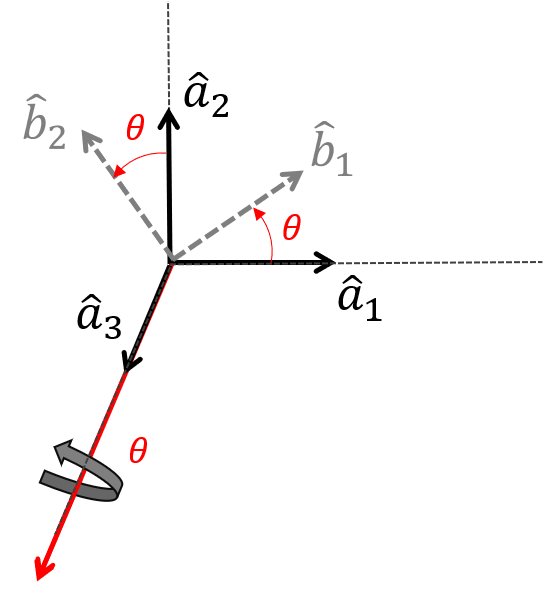
\includegraphics[width=0.30\textwidth]{r3.png}
				\label{fig:r3}}
				\hspace{+20pt}
				\subfloat[Vue de face]{
				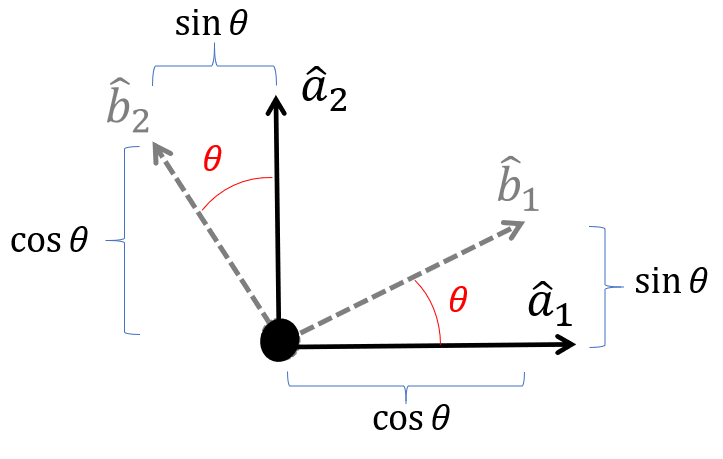
\includegraphics[width=0.40\textwidth]{r3v.png}
				\label{fig:r3v}}
        \caption{Rotation relative selon l'axe 3}
				\label{fig:r3vv}
\end{figure}
%%%%%%%%%%%%%%%%%%%%%%%%%%%%%%%%%%%%%%%%%%%%%%%%%%%%%%%%%%%%%%%%%
%

%%%%%%%%%%%%%%%%%%%%%%%%%%%%%%%%%%%
\subsubsection{Rotation selon l'axe 2}
%
Si les bases vectorielles $a$ et $b$ ont une orientation relative décrite par une rotation d'un angle $\theta$ autour de l'axe 2, les vecteurs unitaires $\hat{a}_2$ et $\hat{b}_2$ sont égaux et, comme illustré à la figure \ref{fig:r2vv}, les quatre autres vecteurs unitaires ($\hat{a}_1$, $\hat{b}_1$, $\hat{a}_3$ et $\hat{b}_3$) sont dans le plan formé par l'axe 1 et l'axe 3. Les vecteurs unitaires sont reliés par des fonctions trigonométriques simples: 
%%%%%%%%%%%%%%%%%%%%
\begin{align}
\hat{b}_1 = c\theta \, \hat{a}_1 -s\theta \, \hat{a}_3 \quad\quad
\hat{b}_2 = \hat{a}_2 \quad\quad
\hat{b}_3 = s\theta \, \hat{a}_1 + c\theta \, \hat{a}_3
\label{eq:rot2vecuni}
\end{align}
%%%%%%%%%%%%%%%%%%%%
La matrice $^aR^b$ peut donc être formée grâce à la définition \eqref{eq:matricerotcol}:
%%%%%%%%%%%%%%%%%%%%
\begin{align}
\col{b}_1^a = \left[ \begin{array}{c} c\theta \\ 0 \\ -s\theta  \end{array} \right] \quad
\col{b}_2^a = \left[ \begin{array}{c} 0 \\ 1 \\ 0  \end{array} \right] \quad
\col{b}_3^a = \left[ \begin{array}{c} s\theta \\ 0 \\ c\theta  \end{array} \right]
\quad \Rightarrow \quad
^aR^b_2(\theta) = \left[ \begin{array}{c c c}
	c\theta  & 0 & s\theta \\
	0        & 1 & 0 \\
	-s\theta & 0 & c\theta 
\end{array}  \right]
\label{eq:rot2theta}
\end{align}
%%%%%%%%%%%%%%%%%%%
%
%%%%%%%%%%%%%%%%%%%%%%%%%%%%%%%%%%%%%%%%%%%%%%%%%%%%%%%%%%%%%%%
\begin{figure}[H]
        \centering
        \subfloat[3D]{
				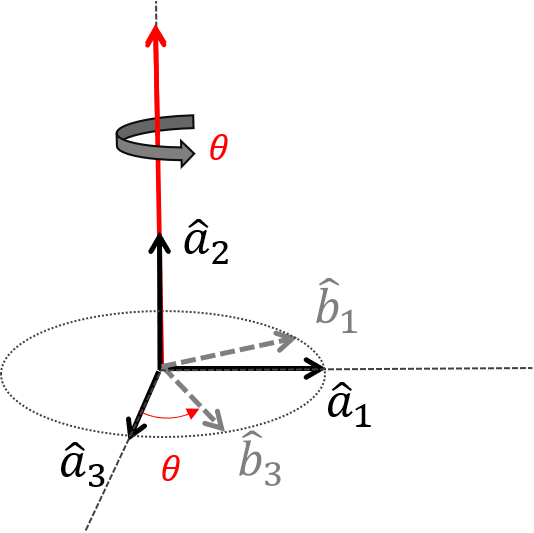
\includegraphics[width=0.30\textwidth]{r2.png}
				\label{fig:r2}}
				\hspace{+20pt}
				\subfloat[Vue de dessus]{
				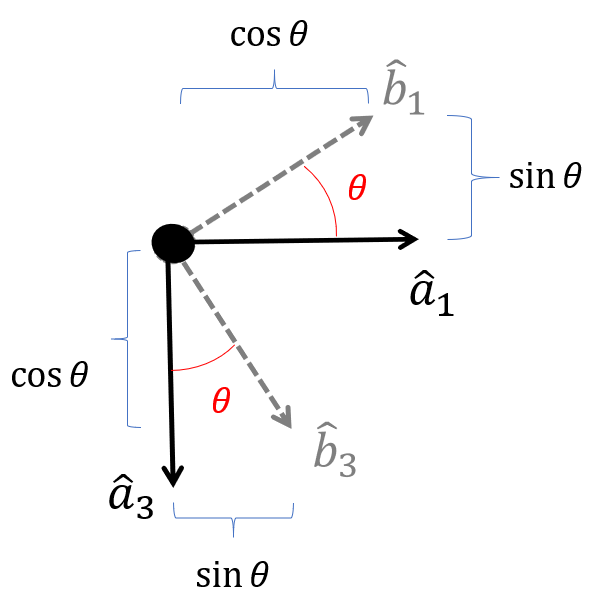
\includegraphics[width=0.30\textwidth]{r2v.png}
				\label{fig:r2v}}
        \caption{Rotation relative selon l'axe 2}
				\label{fig:r2vv}
\end{figure}
%%%%%%%%%%%%%%%%%%%%%%%%%%%%%%%%%%%%%%%%%%%%%%%%%%%%%%%%%%%%%%%%%
%


%%%%%%%%%%%%%%%%%%%%%%%%%%%%%%%%%%%
\subsubsection{Rotation selon l'axe 1}
%
Si les bases vectorielles $a$ et $b$ ont une orientation relative décrite par une rotation d'un angle $\theta$ autour de l'axe 1, les vecteurs unitaires $\hat{a}_1$ et $\hat{b}_1$ sont égaux et, comme illustré à la figure \ref{fig:r3vv}, les quatre autres vecteurs unitaires ($\hat{a}_2$, $\hat{b}_2$, $\hat{a}_3$ et $\hat{b}_3$) sont dans le plan formé par l'axe 2 et l'axe 3. Les vecteurs unitaires sont reliés par des fonctions trigonométriques simples: 
%%%%%%%%%%%%%%%%%%%%
\begin{align}
\hat{b}_1 = \hat{a}_1 \quad\quad
\hat{b}_2 = c\theta \, \hat{a}_2 + s\theta \, \hat{a}_3 \quad\quad
\hat{b}_3 = -s\theta \, \hat{a}_2 + c\theta \, \hat{a}_3
\label{eq:rot1vecuni}
\end{align}
%%%%%%%%%%%%%%%%%%%%
La matrice $^aR^b$ peut donc être formée grâce à la définition \eqref{eq:matricerotcol}:
%%%%%%%%%%%%%%%%%%%%
\begin{align}
\col{b}_1^a = \left[ \begin{array}{c} 1 \\ 0 \\ 0  \end{array} \right] \quad
\col{b}_2^a = \left[ \begin{array}{c} 0 \\ c\theta \\ s\theta  \end{array} \right] \quad
\col{b}_3^a = \left[ \begin{array}{c} 0 \\ -s\theta \\ c\theta  \end{array} \right]
\quad \Rightarrow \quad
^aR^b_1(\theta) 
= \left[ \begin{array}{c c c}
	1 & 0 & 0 \\
	0 & c\theta  & -s\theta \\
	0 & s\theta & c\theta 
\end{array}  \right]
\label{eq:rot1theta}
\end{align}
%%%%%%%%%%%%%%%%%%%%
%
%%%%%%%%%%%%%%%%%%%%%%%%%%%%%%%%%%%%%%%%%%%%%%%%%%%%%%%%%%%%%%%
\begin{figure}[H]
        \centering
        \subfloat[3D]{
				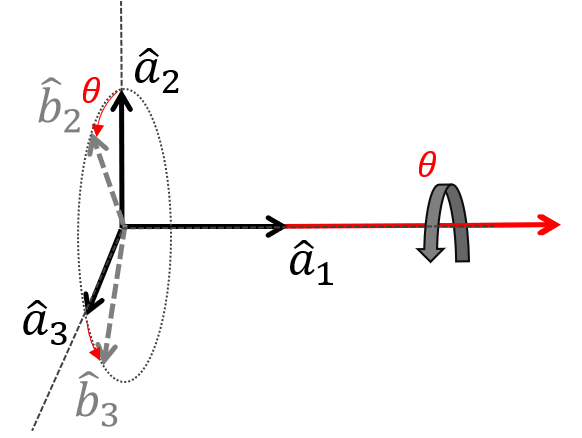
\includegraphics[width=0.30\textwidth]{r1.png}
				\label{fig:r1}}
				\hspace{+20pt}
				\subfloat[Vue de côté]{
				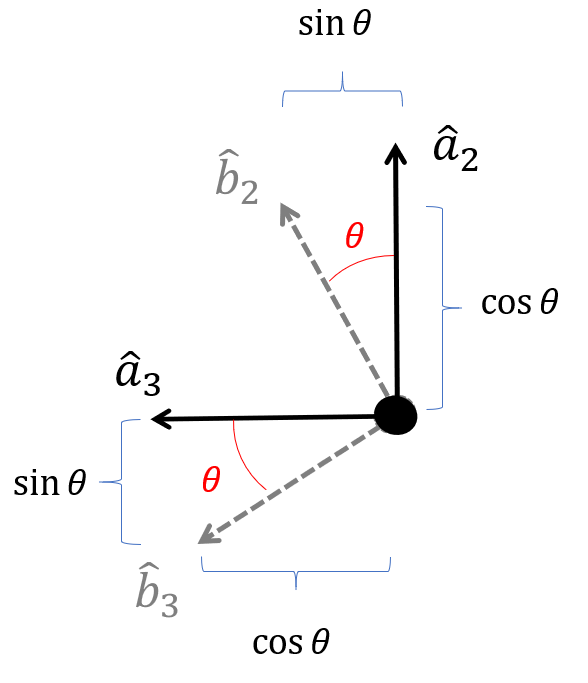
\includegraphics[width=0.30\textwidth]{r1v.png}
				\label{fig:r1v}}
        \caption{Rotation relative selon l'axe 1}
				\label{fig:r1vv}
\end{figure}
%%%%%%%%%%%%%%%%%%%%%%%%%%%%%%%%%%%%%%%%%%%%%%%%%%%%%%%%%%%%%%%%%


%%%%%%%%%%%%%%%%%%%%%%%%%%%%%%%%%%%%%%%%%%%%%%%%%%%%%%%%%%%%%
\subsection{Propriétés des matrices de rotation}

Cette section présente plusieurs propriétés des matrices de rotation qui sont utiles dans un contexte de changement de bases vectorielles.

%%%%%%%%%%%%%%%%%%%%%%%%%%%%%
\subsubsection{Norme des colonnes et rangés}

Les colonnes $\col{c}_i$ et les rangés $\col{r}_i$ d'une matrice de rotation ont une norme égale à 1:
%%%%%%%%%%%%%%%%%%%%%%%%%
\begin{align}
R &= 
\left[ \begin{array}{c c c} 
	\left[ \begin{array}{c} \\ \col{c}_1 \\  \\ \end{array}  \right] & \left[ \begin{array}{c} \\ \col{c}_2 \\  \\ \end{array}  \right] & \left[ \begin{array}{c} \\ \col{c}_3 \\  \\ \end{array}  \right]
\end{array} \right]
=
\left[ \begin{array}{c} 
\left[ \begin{array}{c c c} & \col{r}_1^T & \end{array} \right] \\[\medskipamount]
\left[ \begin{array}{c c c} & \col{r}_2^T & \end{array} \right] \\[\medskipamount]
\left[ \begin{array}{c c c} & \col{r}_3^T & \end{array} \right] 
\end{array} \right] 
\quad \Rightarrow \quad
(\col{c}_i)^T \col{c}_i = 1 \quad \& \quad (\col{r}_i)^T \col{r}_i = 1  \quad \forall i 
\end{align}
%%%%%%%%%%%%%%%%%%%%%%%%%
L’identité trigonométrique suivante est souvent utile pour ce type de calculs:
%%%%%%%%%%%%%%%%%%%%%%%%%
\begin{align}
\sin^2(\theta) + \cos^2(\theta) = 1
\end{align}
%%%%%%%%%%%%%%%%%%%%%%%%%

%%%%%%%%%%%%%%%%%%%%%%%%%%%%%
\subsubsection{Matrice identité}
Une matrice de rotation est réduite à une matrice identitée lorsque les bases vectorielle sont coïncidentes. Par exemple, pour les matrices de rotation élémentaires des équations \eqref{eq:rot3theta}, \eqref{eq:rot2theta} et \eqref{eq:rot1theta}, lorsque l'angle est égale à zéro, les matrices sont réduites à des matrices identités:
%%%%%%%%%%%%%%%%%%%%%%%%%%%%
\begin{align}
R_1( \theta ) = R_2( \theta ) = R_3( \theta ) = I_{3\times3} = 
\left[ \begin{array}{c c c}
	1 & 0 & 0 \\
	0 & 1 & 0 \\
	0 & 0 & 1 
\end{array}  \right]  \quad\text{si}\quad \theta = 0
\label{eq:rot3thetaident}
\end{align}
%%%%%%%%%%%%%%%%%%%%%

%%%%%%%%%%%%%%%%%%%%%%%%%%%%%
\subsubsection{Inversion}

Pour inverser la direction d'une opération de changement de base, il suffit de multiplier par l'inverse de la matrice de rotation:
%%%%%%%%%%%%%%%%%%%%%%%%
\begin{align}
\col{r}^a &= {}^aR^b \, \col{r}^b \\
({}^aR^b)^{-1} \, \col{r}^a &= ({}^aR^b)^{-1} \, {}^aR^b \, \col{r}^b  \\
({}^aR^b)^{-1} \, \col{r}^a &= \col{r}^b
\end{align}
%%%%%%%%%%%%%%%%%%%%%%%%%%%%%%
L'inversion d'une matrice de rotation est équivalente à inverser le signe de l'angle $\theta$ utilisé dans le calcul de la matrice, à prendre la transposée de la matrice et, en termes de notation, à inverser les bases:
%%%%%%%%%%%%%%%%%%%%%%%%
\begin{align}
R(\theta)^{-1} &= R(-\theta) \\
R^{-1} &= R^T \\
({}^bR^a)^{-1} &= {}^aR^b
\end{align}
%%%%%%%%%%%%%%%%%%%%%%%%%%%%%%
%\paragraph{Exercices de lecture}: Vérifiez ces propriétés pour la matrice exemple donnée à l'équation \eqref{eq:rot3theta}.


%%%%%%%%%%%%%%%%%%%%%%%%%%%%%%%%%%%%%%%%%%%%%%%%%%%%%%%%
\subsubsection{Changements de base successifs} 

Des changements de base successifs $a \rightarrow b \rightarrow c \rightarrow ... \rightarrow z$  peuvent être combinés en une seule matrice de rotation en multipliant les matrices de rotation intermédiaires par la gauche:
%%%%%%%%%%%%%%%%%%%
\begin{align}
{}^cR^a &=  {}^cR^b \, {}^bR^a \\
{}^dR^a &=  {}^dR^c \, {}^cR^b \, {}^bR^a \\
& \vdots \\
{}^zR^a &=  {}^zR^y \, {}^yR^x \, \hdots \, {}^cR^b \, {}^bR^a 
\end{align}
%%%%%%%%%%%%%%%%%%%
Notez que selon la notation utilisée dans ces notes, \textbf{les lettres des bases intermédiaires doivent être côte-à-côte dans les équations}, et la matrice de rotation totale conserve la première et la dernière base de la séquence dans le même ordre. Cette propriété découle des définitions, en combinant deux changements de base intermédiaires, une matrice totale peut être obtenue: 
%%%%%%%%%%%%%%%%%%%
\begin{align}
\left. \begin{array}{c}
\col{r}^b = {}^bR^a \col{r}^a \\  \col{r}^c = {}^cR^b \col{r}^b \\ \col{r}^c = {}^cR^a \col{r}^a 
\end{array} \right\} \quad \Rightarrow \quad \col{r}^c = \underbrace{{}^cR^b \,  {}^bR^a}_{ {}^cR^a } \col{r}^a \quad \Rightarrow \quad {}^cR^a  = {}^cR^b \,  {}^bR^a 
\end{align}
%%%%%%%%%%%%%%%%%%

%%%%%%%%%%%%%%%%%%%%%%%%%%%%%
\subsubsection{Non-commutativité}

Le produit des matrices de rotation n'est toutefois pas commutatif, sauf pour des petites rotations infinitésimales. L'ordre de multiplication des matrices est donc important et généralement:
%%%%%%%%%%%%%%%%%%%%%%
\begin{equation}
^cR^b \, ^bR^a \ne {}^bR^a \, ^cR^b
\end{equation} 
%%%%%%%%%%%%%%%%%%%%%%%
Une \textbf{exception à cette règle} est pour les rotations successives selon le même axe de rotation. Par exemple pour deux matrices de rotation élémentaires selon un axe $i$:
%%%%%%%%%%%%%%%%%%%%%%
\begin{equation}
R_i( \theta_1 ) R_i( \theta_2 )  = R_i( \theta_2 ) R_i( \theta_1 ) = R_i( \theta_1 + \theta_2 )
\end{equation} 
%%%%%%%%%%%%%%%%%%%%%%%



%%%%%%%%%%%%%%%%%%%%%%%%%%%%%%%%%%%%%%%%%%%%%%%%%%%%%%%%%%%%
\subsection{Exemple: réorganisation des vecteurs unitaires}
%
La figure \ref{fig:r_reorg} illustre deux bases vectorielles qui ont des vecteurs unitaires parallèles mais avec des directions et un ordre différents. Pour calculer la matrice de rotation associée $^bR^a$, la première étape est d'identifier la relation entre les vecteurs unitaires $\hat{a}_i$ et $\hat{b}_i$. 
%
%%%%%%%%%%%%%%%%%%%%%%%%%%%%%%%%%%%%%%%%%%%%%%%%%%%%%%%%%%%%%%%
\begin{figure}[H]
				%\vspace{-10pt}
        \centering
				\subfloat[Vue 3D]{
				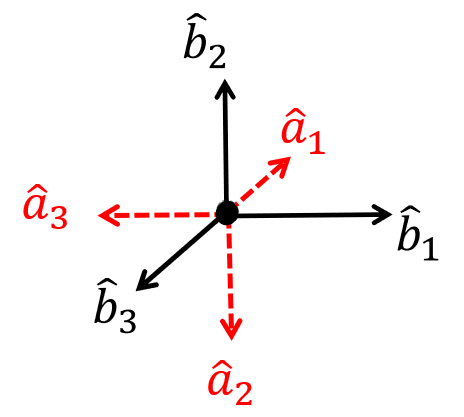
\includegraphics[width=0.25\textwidth]{r_reorg_3d}
				\label{fig:r_reorg_3}}
				%%%%
				\hspace{20pt}
				%%%%
        \subfloat[Vue de face]{
				\includegraphics[width=0.25\textwidth]{r_reorg_face}
				\label{fig:r_reorg_face}}
				%%%%
				\hspace{20pt}
				%%%%
				\subfloat[Vue de dessus]{
				\includegraphics[width=0.25\textwidth]{r_reorg_top}
				\label{fig:r_reorg_top}}
        \caption{Réorganisation des directions des vecteurs unitaires}
				\label{fig:r_reorg}
\end{figure}
%%%%%%%%%%%%%%%%%%%%%%%%%%%%%%%%%%%%%%%%%%%%%%%%%%%%%%%%%%%%%%%%%
%
On peut constater que le vecteur unitaire $\hat{a}_1=-\hat{b}_3$, le vecteur unitaire $\hat{a}_2=-\hat{b}_2$ et le vecteur unitaire $\hat{a}_3=-\hat{b}_1$. Avec ces résultats il est possible d'assembler les vecteur-colonnes $\col{a}_i^b$:
%%
%%%%%%%%%%%%%
\begin{align}
\col{a}_1^b = \left[ \begin{array}{c} 0 \\ 0 \\ -1  \end{array} \right] \quad
\col{a}_2^b = \left[ \begin{array}{c} 0 \\ -1 \\ 0 \end{array} \right] \quad
\col{a}_3^b = \left[ \begin{array}{c} -1 \\ 0 \\ 0   \end{array} \right]
\end{align}
%%%%%%%%%%%%%
%%
Il est donc maintenant possible d'assembler la matrice de rotation $^bR^a$ basée sur l'équation \eqref{eq:matricerotcol}:
%%
%%%%%%%%%%%%
\begin{align}
^bR^a =\left[ \begin{array}{c c c}
	\col{a}_1^b  & \col{a}_2^b & \col{a}_3^b
\end{array}  \right]
= \left[ \begin{array}{c c c}
	0 & 0 & -1 \\
	0 & -1 & 0 \\
-1 & 0 & 0 
\end{array}  \right]
%\label{eq:rot3theta}
\end{align}
%%%%%%%%%%%%




%%%%%%%%%%%%%%%%%%%%%%%%%%%%%%%%%%%%%%%%%%%%%%%%%%%%%%%%%%%%
\subsection{Exemple: réorganisation des vecteurs unitaires et rotation selon un axe}
%
Un exemple de calcul d'une matrice de rotation $^bR^a$ est donné pour une base $a$ qui subit une révolution de $\theta$ degrés autour de l'axe $\hat{b}_3$ par rapport à une base $b$, mais ici avec des vecteurs unitaires qui sont définis avec des directions différentes, tel qu'illustré à la figure \ref{fig:rot3}, et ce n'est donc pas un cas de rotation élémentaire. Pour construire la matrice de rotation, la première étape est de dessiner les deux bases avec une origine commune, dans une configuration où la rotation $\theta$ est relativement faible (pour simplifier la visualisation). On peut constater que le vecteur unitaire $\hat{a}_1$ est aligné avec l'axe de rotation, donc indépendant de $\theta$ et toujours donné par $\hat{a}_1=-\hat{b}_3$. Ensuite, par inspection, il est possible d'exprimer chaque vecteur unitaire $\hat{a}_i$ comme une combinaison des vecteurs unitaires $\hat{b}_i$, avec des relations trigonométriques simples comme illustrés par les figures \ref{fig:rot3_a1} et \ref{fig:rot3_a2}. 
%
%%%%%%%%%%%%%%%%%%%%%%%%%%%%%%%%%%%%%%%%%%%%%%%%%%%%%%%%%%%%%%%
\begin{figure}[H]
				%\vspace{-10pt}
        \centering
				\subfloat[Base vectorielles $a$ et $b$]{
				\includegraphics[width=0.25\textwidth]{rot3}
				\label{fig:rot3}}
				%%%%
				\hspace{20pt}
				%%%%
        \subfloat[Calcul de $\col{a}_3^b$]{
				\includegraphics[width=0.25\textwidth]{rot3_a3}
				\label{fig:rot3_a1}}
				%%%%
				\hspace{20pt}
				%%%%
				\subfloat[Calcul de $\col{a}_2^b$]{
				\includegraphics[width=0.25\textwidth]{rot3_a2}
				\label{fig:rot3_a2}}
        \caption{Rotation selon l'axe 3 et réorganisation des directions des vecteurs unitaires}
				\label{fig:rot3_a2}
\end{figure}
%%%%%%%%%%%%%%%%%%%%%%%%%%%%%%%%%%%%%%%%%%%%%%%%%%%%%%%%%%%%%%%%%
%
Avec ces résultats il est possible d'assembler les vecteur-colonnes $\col{a}_i^b$:
%%
%%%%%%%%%%%%%
\begin{align}
\col{a}_1^b = \left[ \begin{array}{c} 0 \\ 0 \\ -1  \end{array} \right] \quad
\col{a}_2^b = \left[ \begin{array}{c} -s\theta \\ c\theta \\ 0 \end{array} \right] \quad
\col{a}_3^b = \left[ \begin{array}{c} c\theta \\ s\theta \\ 0   \end{array} \right]
\end{align}
%%%%%%%%%%%%%
%%
Il est donc maintenant possible d'assembler la matrice de rotation $^bR^a$ basé sur l'équation \eqref{eq:matricerotcol}:
%%
%%%%%%%%%%%%
\begin{align}
^bR^a =\left[ \begin{array}{c c c}
	\col{a}_1^b  & \col{a}_2^b & \col{a}_3^b
\end{array}  \right]
= \left[ \begin{array}{c c c}
	0 & -s\theta & c\theta \\
	0 & c\theta & s\theta \\
-1 & 0 & 0 
\end{array}  \right]
%\label{eq:rot3theta}
\end{align}
%%%%%%%%%%%%

%%%%%%%%%%%%%%%%%%%%%%%%%%%%%%%%%%%%%%%%%%%%%%%%%%
\subsection{Exemple: calcul de la position globale de l'effecteur d'un robot (suite) }
\label{sec:exer-cinematique-base2}
%
L'exemple \ref{sec:exer-cinematique-base} est ici complété avec le calcul des matrices de rotation. Grâce à une inspection des mouvements relatifs des bases vectorielles, comme illustrée à la figure \ref{fig:vecposrot2}, les matrices de rotation peuvent être calculées. Puisque le robot est planaire, les bases vectorielles $b$, $c$ et $d$ fixées aux pièces mobiles du robot ont tous une rotation relative autour de l'axe $\hat{a}_3$ par rapport à la base vectorielle fixe $a$, tel qu'illustré à la figure \ref{fig:exer-cinematique-base-rotation}.  
%
%%%%%%%%%%%%%%%%%%%%%%%%%%%%%%%%%%%%%%%%%%%%%%%%%%%%%%%%%%%%%%%
\begin{figure}[H]
				%\vspace{-10pt}
        \centering
        \subfloat[$^aR^b$]{
				\includegraphics[width=0.20\textwidth]{baseext1}
				\label{fig:baseext1}}
				\hspace{10pt}
				\subfloat[$^aR^c$]{
				\includegraphics[width=0.20\textwidth]{baseext2}
				\label{fig:baseext2}}
				\hspace{10pt}
				\subfloat[$^aR^d$]{
				\includegraphics[width=0.20\textwidth]{baseext3}
				\label{fig:baseext3}}
        \caption{Calcul des matrices de rotation pour l'exemple \ref{sec:exer-cinematique-base}}
				\label{fig:exer-cinematique-base-rotation}
\end{figure}
%%%%%%%%%%%%%%%%%%%%%%%%%%%%%%%%%%%%%%%%%%%%%%%%%%%%%%%%%%%%%%%%%
%
En fonction des angles définis à la figure \ref{fig:vecposrot3}, les matrices de rotation sont donc toutes des matrices élémentaires de rotation autour de l'axe 3:
%%%%%%%%%%%%%%%%%%%%%%%%%%%%%%%%%%%
\begin{align}
{}^aR^b =
\left[ \begin{array}{c c c}
	c\theta_1 & -s\theta_1 & 0 \\
	s\theta_1 & c\theta_1 & 0 \\
	0 & 0 & 1 
\end{array}  \right]
\quad \quad
 {}^aR^c =
\left[ \begin{array}{c c c}
	c\theta_2 & -s\theta_2 & 0 \\
	s\theta_2 & c\theta_2 & 0 \\
	0 & 0 & 1 
\end{array}  \right]
\quad \quad
{}^aR^d =
\left[ \begin{array}{c c c}
	c\theta_3 & -s\theta_3 & 0 \\
	s\theta_3 & c\theta_3 & 0 \\
	0 & 0 & 1 
\end{array}  \right]
\end{align} 
%%%%%%%%%%%%%%%%%%%%%%%%%%%%%%%%%%%
Ces résultats peuvent donc être substitués dans l'équation matricielle qui avait été obtenue à l'exemple \ref{sec:exer-cinematique-base}:
%%%%%%%%%%%%%%%%%%%%%%%%%%%%%%%%%%%
\begin{align}
\col{r}_{D/A}^a &= {}^aR^d \, \col{r}_{D/C}^d + {}^aR^c \, \col{r}_{C/B}^c + {}^aR^b \, \col{r}_{B/A}^b
\label{eq:ex333cinematique-2}
\end{align} 
%%%%%%%%%%%%%%%%%%%%%%%%%%%%%%%%%%%
et on obtient l’expression précise qui permet de calculer la position du point $D$ par rapport au point de référence $A$ exprimée dans la base vectorielle $a$ en fonction des variables de distances $l_i$ et d'angles $\theta_i$:
%%%%%%%%%%%%%%%%%%%%%%%%%%%%%%%%%%%
\begin{align}
\col{r}_{D/A}^a &= \left[ \begin{array}{c c c}
	c\theta_3 & -s\theta_3 & 0 \\
	s\theta_3 & c\theta_3 & 0 \\
	0 & 0 & 1 
\end{array}  \right] \, \left[ \begin{array}{c} 
0 \\ l_3 \\ 0
\end{array} \right] + \left[ \begin{array}{c c c}
	c\theta_2 & -s\theta_2 & 0 \\
	s\theta_2 & c\theta_2 & 0 \\
	0 & 0 & 1 
\end{array}  \right] \, \left[ \begin{array}{c} 
0 \\ l_2 \\ 0
\end{array} \right]  + \left[ \begin{array}{c c c}
	c\theta_1 & -s\theta_1 & 0 \\
	s\theta_1 & c\theta_1 & 0 \\
	0 & 0 & 1 
\end{array}  \right] \, \left[ \begin{array}{c} 
l_1 \\ 0 \\ 0
\end{array} \right] \\
\col{r}_{D/A}^a &= \left[ \begin{array}{c}
-s\theta_3 l_3 - s\theta_2 l_2  + c\theta_1 l_1 \\
c\theta_3 l_3 + c\theta_2 l_2  + s\theta_1 l_1  \\
0
\end{array} \right]
\label{eq:robot2dpos}
\end{align} 
%%%%%%%%%%%%%%%%%
À noter que ici les angles $\theta_i$ sont tous des angles absolus qui représentent l'orientation des bases $b$, $c$ et $d$ du robot par rapport à la base fixe $a$ directement.

%%%%%%%%%%%%%%%%%%%%%%%%%%%%%%%%%%%%%%%%%%%%%%%%%%%%%%%%%%%%%%%
\begin{figure}[H]
				%\vspace{-10pt}
        \centering
				\subfloat[Construction géométrique]{
				\includegraphics[width=0.30\textwidth]{vecposcons}
				\label{fig:vecposrot1}}
				%%%%
				\hspace{10pt}
				%%%%
        \subfloat[Bases vectorielles]{
				\includegraphics[width=0.27\textwidth]{vecposbase}
				\label{fig:vecposrot2}}
				%%%%
				\hspace{10pt}
				%%%%
        \subfloat[Angles]{
				\includegraphics[width=0.27\textwidth]{vecposbaseangle}
				\label{fig:vecposrot3}}
        \caption{Utilisation des bases vectorielles pour les vecteurs de position}
				\label{fig:vecposrot}
\end{figure}
%%%%%%%%%%%%%%%%%%%%%%%%%%%%%%%%%%%%%%%%%%%%%%%%%%%%%%%%%%%%%%%%%

\textbf{Exercice de lecture: } La hauteur du robot correspond à la deuxième ligne de l'équation \eqref{eq:robot2dpos}, qui est la distance $\vec{r}_{D/A}$ selon le vecteur unitaire $\hat{a}_2$: 
%%%%%%%%%%%%%%%%%%%%%%%%%%%%%%%%%%%
\begin{align}
h = c\theta_3 l_3 + c\theta_2 l_2  + s\theta_1 l_1  
\end{align} 
%%%%%%%%%%%%%%%%%
Alternativement, à l'exemple \ref{sec:hauteurrobot}, l'équation suivante avait été obtenue pour la hauteur du robot:
%%%%%%%%%%%%%%%%%%%%%%%%%%%%%%%%%%%
\begin{align}
h &= l_1 \cos (\varphi_1) + l_2 \cos (\varphi_2) + l_3 \cos (\varphi_3)
\end{align} 
%%%%%%%%%%%%%%%%%%%%%%%%%%%%%%%%%%%
Trouvez la correspondance entre les angles $\theta_i$ et $\varphi_i$ et vérifiez que les deux expressions sont équivalentes.





%%%%%%%%%%%%%%%%%%%%%%%%%%%%%%%%%%%%%%%%%%%%%%%%%%%%%%%%%%%%%%%%%%%%%%%%%%%%%%%%%%%%%%%%%%%%%%%%%%%%%%%%%%%%%%%%%%%%%%%%%%%%%%%%%%%%%%%%%%%%%%%%%%%%%%%%%%
\newpage
\section{Coordonnées dans un repère et transformations homogènes}
\label{sec:repere}

En robotique, il est souvent utile de placer un point de référence ainsi qu'une base vectorielle sur chaque corps rigide du robot. Bien qu'on peut travailler avec des points de référence et des bases vectorielles de façon indépendante, il est souvent pratique de les jumeler en paires puisqu'il faut ces deux types de références pour exprimer des coordonnées. \textbf{La combinaison d'un point d'origine et d'une base vectorielle est appelée repère dans ces notes}, le terme \textit{Frame} est généralement utilisé en anglais. Un repère $A$ dans ces notes fait donc référence à la fois à un point d'origine $A_o$ et à une base vectorielle $a$ qui consiste des trois vecteurs unitaires $\{ \hat{a}_1, \hat{a}_2, \hat{a}_3 \}$. Autrement dit, on appellera \textit{repère} $A$ le repère formé par l'ensemble $\{ A_o, \hat{a}_1, \hat{a}_2, \hat{a}_3 \}$. 
%%%%%%%%%%%%%%%%%%%%%%%%%%%%%%%%%%%%%%%%%%%%%%%%%%%%%%%%%%%%%%%%%%%%%%%%%%%%%
\begin{figure}[htpb]
	\centering
		\includegraphics[width=0.45\textwidth]{repere}
	\caption{Système de coordonnées cartésiennes $(x,y,z)$ basé sur le repère $\{A_o,\hat{a}_1,\hat{a}_2,\hat{a}_3\}$}
	\label{fig:repere}
\end{figure}
%%%%%%%%%%%%%%%%%%%%%%%%%%%%%%%%%%%%%%%%%%%%%%%%%%%%%%%%%%%%%%%%%%%%%%%%%%%%%%%

Comme illustré à la figure \ref{fig:repere}, les coordonnées cartésiennes ($x$, $y$, $z$) d'un point $P$ correspondent directement aux composantes du vecteur position avec comme origine l'intersection des axes du système de coordonnées (le point $A_o$) et exprimé dans une base vectorielle $a$ alignée sur les axes du système de coordonnées:
%%%%%%%%%%%%%%%%%%%%%%%%%%%%%%%%%%%
\begin{align}
\col{r}_{P/A_o}^a = \left[ \begin{array}{c} 
x \\ y \\ z
\end{array} \right]   \quad \Leftrightarrow \quad
\vec{r}_{P/A_o} = x \, \hat{a}_{1} + y \, \hat{a}_{2} + z \, \hat{a}_{3}
\end{align} 
%%%%%%%%%%%%%%%%%%%%%%%%%%%%%%%%%%%
Un système de coordonnées est toujours implicitement attaché à un repère, même s'il n'est pas explicitement défini. L'ensemble de l'origine des axes et des vecteurs unitaires alignés sur ces axes forment un repère. 

%Pour modéliser un bras robotique, il est utile de définir un repère sur chaque corps rigides, car les coordonnées des différents points d’intérêts sont constantes quand elles sont exprimées dans des repères locaux.


%%%%%%%%%%%%%%%%%%%%%%%%%%%%%%%%%%%%%%%%%%%%%%%%%%%%%%%%%%%%%%%%%
\subsection{Changement de repère}
\label{sec:repchan}

Un changement de repère implique deux opérations: \textbf{1)} un changement de l'origine utilisée pour les vecteurs de position et \textbf{2)} un changement de la base vectorielle utilisée pour exprimer les composantes de ce vecteur position. 
%%%%%%%%%%%%%%%%%%%%%%%%%%%%%%%%%%%%%%%%%%%%%%%%%%%%%%%%%%%%%%%
\begin{figure}[htpb]
				%\vspace{-10pt}
        \centering
				\subfloat[Deux systèmes de coordonnées]{
				\includegraphics[width=0.40\textwidth]{repchaA}
				\label{fig:repchaA}}
				%%%%
				\hspace{10pt}
				%%%%
				\subfloat[Construction géométrique]{
				\includegraphics[width=0.40\textwidth]{repchaB}
				\label{fig:repchaB}}
        \caption{Changement du repère $\{B_o,\hat{b}_1,\hat{b}_2,\hat{b}_3\}$ vers  le repère $\{A_o,\hat{a}_1,\hat{a}_2,\hat{a}_3\}$}
				\label{fig:repcha}
\end{figure}
%%%%%%%%%%%%%%%%%%%%%%%%%%%%%%%%%%%%%%%%%%%%%%%%%%%%%%%%%%%%%%%%%
Comme illustré à la figure \ref{fig:repcha} pour une transformation d'un repère B vers un repère A, les coordonnées cartésiennes d'un point $C$ correspondent au vecteur-colonne $\col{r}_{C/B_o}^b$ dans le repère B et au vecteur-colonne $\col{r}_{C/A_o}^a$ dans le repère A:
%%%%%%%%%%%%%%%%%%%%%%%%%%%%%%%%%%%
\begin{align}
\col{r}_{C/B_o}^b = 
\left[ \begin{array}{c} 
x \\ y \\ z
\end{array} \right]  \quad \quad
\col{r}_{C/A_o}^a = 
\left[ \begin{array}{c} 
X \\ Y \\ Z
\end{array} \right] 
\end{align} 
%%%%%%%%%%%%%%%%%%%%%%%%%%%%%%%%%%%
Pour effectuer la transformation des coordonnées ($x$, $y$, $z$) vers les coordonnées ($X$, $Y$, $Z$), la première étape est de construire la relation vectorielle qui relie les trois points:
%%%%%%%%%%%%%%%%%%%%%%%%%%%%%%%%%%%
\begin{align}
\vec{r}_{C/A_o}   &= \vec{r}_{C/B_o}  + \vec{r}_{B_o/A_o} 
\end{align} 
%%%%%%%%%%%%%%%%%%%%%%%%%%%%%%%%%%%
et ensuite il suffit de tout exprimer ces vecteurs dans la base $a$ pour effectuer l'addition:
%%%%%%%%%%%%%%%%%%%%%%%%%%%%%%%%%%%
\begin{align}
\col{r}_{C/A_o}^a &=         \col{r}_{C/B_o}^a  + \col{r}_{B_o/A_o}^a  \\
\col{r}_{C/A_o}^a &= {}^aR^b \col{r}_{C/B_o}^b  + \col{r}_{B_o/A_o}^a 
\label{eq:reperechang}
\end{align} 
%%%%%%%%%%%%%%%%%%%%%%%%%%%%%%%%%%%
ce qui correspond en termes de coordonnées à: 
%%%%%%%%%%%%%%%%%%%%%%%%%%%%%%%%%%%
\begin{align}
\left[ \begin{array}{c} 
X \\ Y \\ Z
\end{array} \right]  &=  
 {}^aR^b
\left[ \begin{array}{c} 
x \\ y \\ z
\end{array} \right] + \col{r}_{B_o/A_o}^a 
\end{align} 
%%%%%%%%%%%%%%%%%%%%%%%%%%%%%%%%%%%
Un changement de base est nécessaire puisque que le vecteur $\vec{r}_{C/B_o}$ est connu dans la base vectorielle $b$. Donc les informations nécessaires pour effectuer la transformation sont: \textbf{1)} les composantes $\col{r}_{B_o/A_o}^a$ du vecteur position qui relie les origines $A_o$ et $B_o$ et 2\textbf{)} la matrice de rotation $^aR^b$ qui donne l'orientation relative des bases vectorielles $a$ et $b$. 

L'\textbf{opération inverse} s'obtient à partir de l'équation \eqref{eq:reperechang}, d'abord on soustrait le vecteur translation $\col{r}_{B_o/A_o}^a$ et on multiplie par la gauche l'inverse de la matrice de rotation pour obtenir:
%%%%%%%%%%%%%%%%%%%%%%%%%%%%%%%%%%%
\begin{align}
\col{r}_{C/B_o}^b &= {}^bR^a \; \col{r}_{C/A_o}^a - {}^bR^a \; \col{r}_{B_o/A_o}^a 
\label{eq:reperechanginv}
\end{align} 
%%%%%%%%%%%%%%%%%%%%%%%%%%%%%%%%%%%
ce qui correspond en termes des coordonnées à: 
%%%%%%%%%%%%%%%%%%%%%%%%%%%%%%%%%%%
\begin{align}
\left[ \begin{array}{c} 
x \\ y \\ z
\end{array} \right]  &=  
 {}^bR^a
\left[ \begin{array}{c} 
X \\ Y \\ Z
\end{array} \right] + {}^bR^a \; \col{r}_{B_o/A_o}^a 
\end{align} 
%%%%%%%%%%%%%%%%%%%%%%%%%%%%%%%%%%%




%%%%%%%%%%%%%%%%%%%%%%%%%%%%%%%%%%%%%%%%%%%%%%%%%%
\subsection{Coordonnées et transformations homogènes}
\label{sec:coordhomo}

Dans les logiciels de cinématique et de graphique, les opérations de changement de repère peuvent être très fréquentes. Il existe une méthode standard pour combiner l'opération d'addition vectorielle et la multiplication avec la matrice de rotation en une seule opération équivalente qui consiste à multiplier une matrice de transformation $4\times4$ notée $^AT^B$, avec un vecteur-colonne $4\times1$ de \textit{coordonnées homogènes}. Les coordonnées homogènes sont tout simplement les coordonnées cartésiennes pour les trois premières composantes et la valeur 1 pour la quatrième composante. 

Le changement de repère décrit à la section \ref{sec:repchan} correspond alors à l'opération suivante:
%%%%%%%%%%%%%%%%%%%%%%%%%%%%%%%%%%%
\begin{align}
\left[ \begin{array}{c} 
\col{r}_{C/A_o}^a \\ 1
\end{array} \right] 
= 
\underbrace{
\left[ \begin{array}{c c } 
^aR^b & \col{r}_{B_o/A_o}^a \\ 0 \; 0 \; 0 & 1
\end{array} \right] 
}_{^AT^B}
\left[ \begin{array}{c} 
\col{r}_{C/B_o}^b \\ 1
\end{array} \right] 
\label{eq:homo1}
\end{align} 
%%%%%%%%%%%%%%%%%%%%%%%%%%%%%%%%%%%
ce qui correspond en termes de coordonnées à:
%%%%%%%%%%%%%%%%%%%%%%%%%%%%%%%%%%%
\begin{align}
\left[ \begin{array}{c} 
X \\ Y \\ Z \\ 1
\end{array} \right] 
= 
\underbrace{
\left[ \begin{array}{c c } 
^aR^b & \col{r}_{B_o/A_o}^a \\ 0 \; 0 \; 0 & 1
\end{array} \right] 
}_{^AT^B}
\left[ \begin{array}{c} 
x \\ y \\ z \\ 1
\end{array} \right] 
\label{eq:homo2}
\end{align} 
%%%%%%%%%%%%%%%%%%%%%%%%%%%%%%%%%%%
Les trois premières rangés des équations matricielles \eqref{eq:homo1} et \eqref{eq:homo2} correspondent exactement à l'équation \eqref{eq:reperechang}, et la dernière ligne correspond simplement à une équation 1=1. Les transformations homogènes c'est donc rien de fondamentalement nouveau, mais une astuce bien utile dans un contexte de programmation pour grouper deux opérations en une seule. %D'autre types d'opérations peuvent aussi être exprimés sous la forme d'une multiplication d'une matrice de transformation 4x4 sur un vecteur-colonne 4x1 de coordonnées homogènes. 

Si on substitut les définitions, la matrice de transformation peut être définie directement en termes de vecteurs de vecteurs unitaires et du vecteur géométrique qui définie la translation d'une origine à l'autre:
%%%%%%%%%%%%%%%%%%%%%%%%%%%%%%%%%%%
\begin{align}
{}^AT^B &= 
\left[ \begin{array}{c c } 
^aR^b & \col{r}_{B_o/A_o}^a \\ 0 \; 0 \; 0 & 1
\end{array} \right] 
=
\left[ \begin{array}{c c c c} 
\hat{a}_1 \bullet \hat{b}_1  &  \hat{a}_1 \bullet \hat{b}_2  &  \hat{a}_1 \bullet \hat{b}_3 & \hat{a}_1 \bullet \vec{r}_{B_o/A_o} \\
\hat{a}_2 \bullet \hat{b}_1  &  \hat{a}_2 \bullet \hat{b}_2  &  \hat{a}_2 \bullet \hat{b}_3 & \hat{a}_2 \bullet \vec{r}_{B_o/A_o}\\
\hat{a}_3 \bullet \hat{b}_1  &  \hat{a}_3 \bullet \hat{b}_2  &  \hat{a}_3 \bullet \hat{b}_3 & \hat{a}_3 \bullet \vec{r}_{B_o/A_o} \\
0 & 0 & 0 & 1
\end{array} \right] 
\label{eq:transformationdef}
\end{align} 
%%%%%%%%%%%%%%%%%%%%%%%%%%%%%%%%%%%


L'\textbf{opération inverse} de changement de repère avec les coordonnées homogènes est formée par:
%%%%%%%%%%%%%%%%%%%%%%%%%%%%%%%%%%%
\begin{align}
\left[ \begin{array}{c} 
\col{r}_{C/B_o}^b \\ 1
\end{array} \right] 
= 
\underbrace{
\left[ \begin{array}{c c } 
^bR^a & - ^bR^a \, \col{r}_{B_o/A_o}^a \\ 0 \; 0 \; 0 & 1
\end{array} \right] 
}_{ ({}^AT^B)^{-1} }
\left[ \begin{array}{c} 
\col{r}_{C/A_o}^a \\ 1
\end{array} \right] 
\end{align} 
%%%%%%%%%%%%%%%%%%%%%%%%%%%%%%%%%%%
Comme pour les matrices de rotation l'inverse de la matrice de transformation correspond à inverser les repères avec la notation utilisée:
%%%%%%%%%%%%%%%%%%%%%%%%%%%%%%%%%%%
\begin{align}
({}^AT^B)^{-1}= {}^BT^A
\end{align} 
%%%%%%%%%%%%%%%%%%%%%%%%%%%%%%%%%%%

Dernièrement, les \textbf{changements de repères successifs} $A \rightarrow B \rightarrow C \rightarrow ... \rightarrow Z$  peuvent être combinés en une seule matrice de transformation en multipliant les matrices de transformation intermédiaires par la gauche:
%%%%%%%%%%%%%%%%%%%%%%%%%%%%%%%%%%%
\begin{align}
{}^CT^A &=  {}^CT^B \, {}^BT^A \\
{}^DT^A &=  {}^DT^C \, {}^CT^B \, {}^BT^A \\
& \vdots \nonumber \\
{}^ZT^A &= {}^ZT^Y \, {}^YT^X \, ... \, {}^CT^B \,  {}^BT^A 
\end{align} 
%%%%%%%%%%%%%%%%%%%%%%%%%%%%%%%%%%%
Avec la notation utilisée dans ces notes, \textbf{les lettres des repères intermédiaires doivent être côte-à-côte dans les équations}, et la matrice de transformation totale conserve le premier et le dernier repère de la séquence dans le même ordre. 




%%%%%%%%%%%%%%%%%%%%%%%%%%%%%%%%%%%%%%%%%%%%%%%%%%%%%%%%%%%%%%%%%
\newpage
\section{Représentation de la pose d'un corps rigide}
\label{sec:corps}

De façon générale, six variables sont nécessaires pour définir la positon d'un corps rigide par rapport à un repère, trois pour décrire la translation et trois pour décrire l'orientation. Pour un corps rigide sans aucune contrainte, par exemple un avion en vol, le nombre de DDL est donc de six. 

%%%%%%%%%%%%%%%%%%%%%%%%%%%%%%%%%%%%%%%%%%%%%%%%%%%%%%%%%%%%%%%%%%%%%%%%%%%%%
\begin{figure}[H]
	\centering
		\includegraphics[width=0.95\textwidth]{rigid.png}
	\caption{Représentation de la pose d'un corp rigide}
	\label{fig:rigid}
\end{figure}
%%%%%%%%%%%%%%%%%%%%%%%%%%%%%%%%%%%%%%%%%%%%%%%%%%%%%%%%%%%%%%%%%%%%%%%%%%%%%%%

\subsubsection{Translation}
%
Les trois DDL de translation peuvent être représentés par un vecteur position qui a comme origine un point fixe $A$ et comme cible un point arbitraire $B$ sur le corps rigide. Ce vecteur position $\vec{r}_{B/A}$, est typiquement représenté avec trois coordonnées cartésiennes ($x$, $y$, $z$) qui utilisent une base vectorielle fixe $a$:
%%%%%%%%%%%%%%%%%%%
\begin{equation}
\col{r}_{B/A}^a = \left[ \begin{array}{c} x \\  y \\ z  \end{array} \right]
\quad \Leftrightarrow  \quad 
\vec{r}_{B/A} = x \, \vec{a}_1 + y \, \vec{a}_2 + z \, \vec{a}_3
\end{equation} 
%%%%%%%%%%%%%%%%%%%%

\subsubsection{Orientation}
%
Ensuite, même avec un point défini dans l'espace par un vecteur translation, un corps rigide a plusieurs orientations possibles. Pour définir l'orientation, une autre base vectorielle $b$ attachée au corps rigide doit être utilisée. L'orientation d'un corps rigide est alors représentée par la direction des vecteurs unitaires $\hat{b}_i$, qui peuvent être représentés par leurs composantes dans la base fixe $a$. Les trois vecteur-colonnes $\col{b}_i^a$ de trois composantes peuvent être regroupés sous la forme d'une matrice de rotation, comme il a été discuté à la section \ref{sec:changematrice} dans le contexte des changements de base:
%%%%%%%%%%%%%%%%%%%
\begin{equation}
^aR^b = \left[ \begin{array}{ c c c } \col{b}_1^a &  \col{b}_2^a & \col{b}_3^a  \end{array} \right] = R(\phi,\theta,\psi)
\end{equation} 
%%%%%%%%%%%%%%%%%%%%

Malgré les neuf composants d'une matrice de rotation, puisque les vecteurs $\hat{b}_i$ sont unitaires et orthogonaux seulement trois variables suffisent pour la définir; il y a un total de neuf composantes et six équations de contraintes, voir les équations \eqref{eq:unit} et \eqref{eq:ortho}. Il est donc possible de paramétrer la matrice $^aR^b$ avec trois variables, par exemple trois angles $\phi$, $\theta$ et $\psi$, sans limiter les orientations possibles. On appelle trois angles qui paramétrisent une matrice de rotation des angles de Euler, diverses conventions de paramétrisation sont possibles et c'est le sujet de la section \ref{sec:angeuler}. Selon la situation, d'autres représentations alternatives aux matrices de rotation et aux angles de Euler peuvent aussi être utiles, chaque représentation a ses avantages et inconvénients. La section \ref{sec:rotaxe} présente la représentation axe-angle et la section \ref{sec:quaternions} présente les quaternions. 

%\paragraph{Note:} L'orientation d'un corps rigide est aussi parfois appelée \textit{attitude}, typiquement dans le domaine de l'aérospatiale, ou bien \textit{position angulaire}.

\subsubsection{Pose}

La pose d'un corps rigide, c'est la combinaison de sa translation et de son orientation. Il est possible d'utiliser des représentations indépendantes pour la translation et l'orientation, mais alternativement on peut regrouper une matrice de rotation (pour représenter l'orientation) et un vecteur-colonne (pour représenter la translation)  sous la forme d'une matrice de transformation 4x4, qui relie le repère $\{A_o,\hat{a}_1,\hat{a}_2,\hat{a}_3\}$ formé par le point fixe et la base fixe, au repère $\{B_o,\hat{b}_1,\hat{b}_2,\hat{b}_3\}$ formé par le point mobile et la base mobile attachés au corps rigide. Cette matrice peut alors être paramétrée par 6 variables qui représent tous les DDL du corps rigide:
%%%%%%%%%%%%%%%%%%%
\begin{equation}
^{A}T^B(x,y,z,\phi,\theta,\psi) = \left[ \begin{array}{c c}
	^aR^b  & \col{r}^a_{B/A} \\ 0 \; 0 \; 0 & 1
\end{array}  \right] = 
\left[ \begin{array}{c c}
\left[	\begin{array}{c} \\  R(\phi,\theta,\psi) \\ \\ \end{array} \right] & \left[ \begin{array}{c} x \\ y \\ z \end{array} \right] \\  \begin{array}{ccc} 0 & 0 & 0 \end{array}   &  1 
\end{array}  \right] 
\end{equation} 
%%%%%%%%%%%%%%%%%%%%

La matrice de transformation $^{A}T^B$ a donc deux fonctions: \textbf{1)} elle peut être utilisée pour effectuer des changements de repères comme vue à la section \ref{sec:coordhomo}, et \textbf{2)} elle peut aussi être utilisée pour représenter la pose d'un repère $B$ (donc aussi la pose du corps rigide sur lequel il est attaché) relativement à un repère $A$.  


%%%%%%%%%%%%%%%%%%%%%%%%%%%%%%%%%%%%%%%%%%%%%%%%%%%%%%%%%%%%%%%%%%%%%%%%%%%%%%%
\subsection{Angles de Euler}
\label{sec:angeuler}

Une matrice de rotation arbitraire peut être paramétrée avec trois variables. La méthode la plus simple pour y parvenir est de construire une matrice de rotation comme une multiplication de trois matrices élémentaires. Par exemple, l'orientation arbitraire d'une base vectorielle $d$ par rapport à une base vectorielle $a$ peut être décrite par les angles $( \phi, \theta, \psi)$, avec la convention 3-1-3:
%%%%%%%%%%%%%%%%%%%
\begin{align}
{}^aR^d(\phi,\theta,\psi) &= R_3(\phi) \, R_1(\theta) \, R_3(\psi) \\
{}^aR^d(\phi,\theta,\psi) &= 
\left[ \begin{array}{c c c}
	c\phi & -s\phi & 0 \\
	s\phi & c\phi & 0 \\
	0 & 0 & 1 
\end{array}  \right]
\left[ \begin{array}{c c c}
	1 & 0 & 0 \\
	0 & c\theta  & -s\theta \\
	0 & s\theta & c\theta 
\end{array}  \right]
\left[ \begin{array}{c c c}
	c\psi & -s\psi & 0 \\
	s\psi & c\psi & 0 \\
	0 & 0 & 1 
\end{array}  \right] \\
{}^aR^d(\phi,\theta,\psi) &= 
\left[ \begin{array}{c c c}
	 + c\phi \, c\psi - s\phi\,c\theta\,c\psi  & - c\phi \, s\psi - s\phi \, c\theta c\psi  & + s\phi \, s\theta  \\
	 + s\phi \, c\psi + c\phi\,c\theta\,c\psi  & - s\phi \, s\psi + c\phi \, c\theta c\psi  & - c\phi \, s\theta  \\
	 + s\theta \, s\psi                        & + s\theta \, c\psi                          & + c\theta 
\end{array}  \right]
\end{align} 
%%%%%%%%%%%%%%%%%%%%
Cette matrice peut être interprétée comme une suite de trois rotations, avec des bases vectorielles intermédiaires, illustrées à la figure \ref{fig:euler}. 
%%%%%%%%%%%%%%%%%%%%%%%%%%%%%%%%%%%%%%%%%%%%%%%%%%%%%%%%%%%%%%%
\begin{figure}[H]
				%\vspace{-10pt}
        \centering
        \subfloat[${}^aR^b=R_3(\phi)$]{
				\includegraphics[width=0.28\textwidth]{euler1}
				\label{fig:euler1}}
				\subfloat[${}^bR^c=R_1(\theta)$]{
				\includegraphics[width=0.30\textwidth]{euler2}
				\label{fig:euler2}}
				\subfloat[${}^cR^d=R_3(\psi)$]{
				\includegraphics[width=0.33\textwidth]{euler3}
				\label{fig:euler3}}
        \caption{Angles de Euler avec la convention 3-1-3: toutes les orientations possibles de la base $d$ peuvent être décrites par la matrice de rotation ${}^aR^d(\phi,\theta,\psi) = R_3(\phi)R_1(\theta)R_3(\psi)$ paramétrisée avec trois angles.}
				\label{fig:euler}
\end{figure}
%%%%%%%%%%%%%%%%%%%%%%%%%%%%%%%%%%%%%%%%%%%%%%%%%%%%%%%%%%%%%%%%%
%
Une autre convention de trois angles utilisée fréquemment en robotique (typiquement pour les véhicules) sont les angles de roulis, tangage et lacet. Ces angles correspondent à une matrice formée par la multiplication de matrices élémentaires dans un ordre 3-2-1, si l'axe 1 correspond à la direction avant-arrière du véhicule et l'axe 2 vers à la direction haut-bas du véhicule: 
%%%%%%%%%%%%%%%%%%%
\begin{align}
R_{321}(\theta_{tangage}, \theta_{lacet}, \theta_{roulis}) &= R_3( \theta_{tangage} ) \, R_2( \theta_{lacet} ) \, R_1( \theta_{roulis} )
\end{align} 
%%%%%%%%%%%%%%%%%%%%

Comme l'ordre des matrices de rotation qui sont multipliées influence la matrice résultante, il y a plusieurs possibilités de définitions des trois angles de Euler qui paramétrisent la matrice. Différents auteurs, domaines et organisations utilisent des définitions différentes, il est donc toujours \textbf{important de vérifier la convention utilisée si on travail avec les angles de Euler}. 





%%%%%%%%%%%%%%%%%%%%%%%%%%%%%%%%%%%%%%%%%%%%%%%%%%%%%%%%%%%%%%%%%%%%%%%%%%%%%%%
\subsection{Représentation axe-angle}
\label{sec:rotaxe}
Une orientation relative entre deux bases vectorielles peut aussi être représentée par un axe de rotation, décris par un vecteur unitaire $\hat{a}$, et un angle $\theta$ de rotation autour de celui-ci, comme illustré à la figure \ref{fig:angleaxis}.
%%%%%%%%%%%%%%%
\begin{figure}[htbp]
	\centering
		\includegraphics[width=0.35\textwidth]{angleaxis.png}
	\caption{Représentation axe-angle d'une orientation relative}
	\label{fig:angleaxis}
\end{figure}
%%%%%%%%%%%%%%%%

Cette représentation nécessite quatre paramètres, trois pour un vecteur-colonne $\col{a}$ qui représente les composantes du vecteur unitaire qui décris l'axe de rotation, et un pour l'angle $\theta$. La représentation axe-angle permet donc d'utiliser seulement 4 variables plutôt que les 9 d'une matrice $3\times3$ pour représenter une rotation dans un espace tridimensionnel. Un paramètre est toutefois redondant, car le vecteur-colonne $\col{a}$ est unitaire et trois variables sont reliés par l'équation $a_{1}^2+a_{2}^2+a_{3}^2=1$. De plus, cette représentation présente des singularités lorsque $sin(\theta)=0$. L'avantage principal de la représentation axe-angle est le sens physique clair. Les inconvénients sont qu'il faut convertir vers des matrices de rotation (ou alternativement des quaternions) pour effectuer des calculs numériques de changement de base et pour combiner des rotations successives.



\subsubsection{Vecteur propre de la matrice de rotation}
L'axe de rotation $\hat{a}$ est directement lié à la matrice de rotation qui représente la même orientation relative entre deux bases vectorielles. Le vecteur unitaire $\hat{a}$ aligné avec l'axe de rotation a les mêmes composantes dans les deux bases vectorielles:
%%%%%%%%%%%%%%%%%%%%%
\begin{equation}
\col{a} = \col{a}^b = {}^bR^a \col{a}^a = {}^aR^b \col{a}^b = \col{a}^a
\end{equation} 
%%%%%%%%%%%%%%%%%%%%%
Le vecteur-colonne qui représente \textbf{l'axe de rotation est donc un vecteur propre de la matrice de rotation}, et la valeur propre associée est de valeur unitaire car le vecteur-colonne est inchangé par la multiplication avec la matrice de rotation. Il est donc possible de calculer l'axe de rotation associé à une matrice de rotation en calculant les valeurs et vecteurs propre de la matrice.

\subsubsection{Convertions}
La représentation axe-angle peut être calculée à partir d'une matrice de rotation $R$ de la façon suivante:
%%%%%%%%%%%%%%%%%%
\begin{equation} 
\theta=cos^{-1}\left[\frac{R_{11}+R_{22}+R_{33}-1}{2}\right]
\quad\quad 
\col{a}=\frac{1}{2 \, sin(\theta)}\left[ \begin{array}{c}
R_{32}-R_{23}  \\ 
R_{13}-R_{31} \\ 
R_{21}-R_{12} \end{array}
\right]
\end{equation}
%%%%%%%%%%%%%%%%%%
où
%%%%%%%%%%%%%%%%%%
\begin{equation}
R =\left[ \begin{array}{ccc}
R_{11} & R_{12} & R_{13} \\ 
R_{21} & R_{22} & R_{23} \\ 
R_{31} & R_{32} & R_{33} \end{array}
\right]
\end{equation}
%%%%%%%%%%%%%%%%%%%
Inversement, la matrice de rotation peut être déterminée à partir de la représentation axe-angle:
%%%%%%%%%%%%%%%%
\begin{equation}
R=cos(\theta) \, I + (1-cos(\theta) ) \, \col{a}\ \col{a}^T-sin(\theta)\col{a}^{\times}
\end{equation}
%%%%%%%%%%%%%%%%%%%%%%%%
où
%%%%%%%%%%%%%%%%%%%%%%%
\begin{equation}
I =\left[ \begin{array}{ccc}
1 & 0 & 0 \\ 
0 & 1 & 0 \\ 
0 & 0 & 1      \end{array}
\right] \quad\quad
\col{a}=\left[ \begin{array}{c}
a_{1}  \\ 
a_{2}  \\ 
a_{3} \end{array}
\right]
\quad\quad
\col{a}^T=\left[ \begin{array}{ccc} a_{1} & a_{2} & a_{3} \end{array} \right]
\quad\quad
\col{a}^{\times} =\left[ \begin{array}{ccc}
0      & -a_{3} &  a_{2} \\ 
 a_{3} & 0      & -a_{1} \\ 
-a_{2} &  a_{1} & 0      \end{array}
\right]
\end{equation}
%%%%%%%%%%%%%%%%%%%%%%%


%%%%%%%%%%%%%%%%%%%%%%%%%%%%%%%%%%%%%%%%%%%%%%%%%%%%%%%%%%%%%%%%%%%%%%%%%%%%%%%
\subsection{Quaternions}
\label{sec:quaternions}
Les quaternions sont une autre façon de représenter une orientation avec 4 paramètres, physiquement moins représentative mais beaucoup plus pratique mathématiquement. Similairement à la représentation axe-angle, un quaternion est constitué d'un scalaire et de 3 composantes vectorielles qui peuvent être groupés dans un vecteur colonne $[\eta,\ e_{1},\ e_{2},\ e_{3}]^T$. Les quatre paramètres sont reliés par l'équation suivante $\eta^2+e_{1}^2+e_{2}^2+e_{3}^2=1$. Cette représentation se dérive facilement à partir de la représentation axe-angle.
%%%%%%%%%%%%%%%%%%%%%
\begin{equation}
\eta=\cos\left(\frac{\theta}{2}\right)
\end{equation}
\begin{equation}
\left[ \begin{array}{c} e_{1} \\ e_{2} \\ e_{3} \end{array}
\right]
=\sin\left(\frac{\theta}{2}\right) \left[ \begin{array}{c} a_{1} \\ a_{2} \\ a_{3} \end{array}
\right]
\end{equation}
%%%%%%%%%%%%%%%%%%%%
Les grands avantages de cette représentation sont \textbf{1)} l'absence de singularité et \textbf{2)} des méthodes numériquement efficaces pour calculer des rotations successives et des changements de base directement avec le vecteur colonne $[\eta,\ e_{1},\ e_{2},\ e_{3}]^T$. 

%TODO
Détails à venir!

%les rotations peuvent être calculées sans utiliser de sinus ou de cosinus. 

%En effet, l'addition de deux rotations est une opération spéciale entre deux quaternions.

%Une succession de deux rotation s'exprime ainsi avec des matrices de rotation $\col{R}^B_0=\col{R}^B_A\col{R}^A_0$ et ainsi avec des quaternions $\textbf{Q}^B_O=\textbf{Q}^B_A*\textbf{Q}^A_O$. L'opérateur $*$ est une multiplication de quaternion définie de la façon suivante :
%\begin{equation}
%\textbf{Q}_A*\textbf{Q}_B=[\eta_A\eta_B-\textbf{e}_A \bullet \textbf{e}_B, \eta_A\textbf{e}_B+\eta_B\textbf{e}_A+\textbf{e}_A\times \textbf{e}_B]
%\end{equation}
%Les quaternions peuvent aussi être utilisés directement pour faire la convertion des composantes d'un vecteur d'un repère à un autre grâce à une opération qui s'écrit ainsi $\col{V}^{'}=\textbf{Q} \col{V} \textbf{Q}^*$.




\newpage
%%%%%%%%%%%%%%%%%%%%%%%%%%%%%%%%%%%%%%%%%%%%%%%%%%%%
\subsection{Exemple: cinématique d'un robot mobile}

La figure illustre un exemple où un véhicule et les points d’intérêts qu'il trouve doivent être localisés par rapport à une base. La cinématique de ce problème peut se résumer à calculer la matrice de transformation $^AT^B$, qui peut être construite à partir de la définition:
%%%%%%%%%%%%%%%%%%%%%%%%%%%%%%%%%%%
\begin{align}
{}^AT^B &= 
\left[ \begin{array}{c c } 
^aR^b & \col{r}_{B_o/A_o}^a \\ 0 \; 0 \; 0 & 1
\end{array} \right] 
=
\left[ \begin{array}{c c c c} 
\hat{a}_1 \bullet \hat{b}_1  &  \hat{a}_1 \bullet \hat{b}_2  &  \hat{a}_1 \bullet \hat{b}_3 & \hat{a}_1 \bullet \vec{r}_{B_o/A_o} \\
\hat{a}_2 \bullet \hat{b}_1  &  \hat{a}_2 \bullet \hat{b}_2  &  \hat{a}_2 \bullet \hat{b}_3 & \hat{a}_2 \bullet \vec{r}_{B_o/A_o}\\
\hat{a}_3 \bullet \hat{b}_1  &  \hat{a}_3 \bullet \hat{b}_2  &  \hat{a}_3 \bullet \hat{b}_3 & \hat{a}_3 \bullet \vec{r}_{B_o/A_o} \\
0 & 0 & 0 & 1
\end{array} \right] 
\label{eq:transformationdef_app}
\end{align} 
%%%%%%%%%%%%%%%%%%%%%%%%%%%%%%%%%%%
Cette matrice représente la pose du véhicule par rapport au repère de la base, et peut aussi être utilisée pour transformer des coordonnées cartésiennes relatives au repère du véhicule en des coordonnées cartésiennes relatives au repère de la base:
%%%%%%%%%%%%%%%%%%%%%%%%%%%%%%%%%%%
\begin{align}
\left[ \begin{array}{c} 
\col{r}_{C/A_o}^a \\ 1
\end{array} \right] 
= 
{}^AT^B
\left[ \begin{array}{c} 
\col{r}_{C/B_o}^b \\ 1
\end{array} \right] 
\label{eq:homo1_app}
\end{align} 
%%%%%%%%%%%%%%%%%%%%%%%%%%%%%%%%%%%

%%%%%%%%%%%%%%%%%%%%%%%%%%%%%%%%%%%%%
\begin{figure}[H]
	\centering
		\includegraphics[width=0.95\textwidth]{vec.png}
	\caption{Cinématique d'un robot mobile}
	\label{fig:vec}
\end{figure}
%%%%%%%%%%%%%%%%%%%%%%%%%%%%%%%%%%%%%



\newpage
%%%%%%%%%%%%%%%%%%%%%%%%%%%%%%%%%%%%%%%%%%%%%%%%%%%%%%%%%%%%%%%%%%%%%%%%%%%%%%%
\section{Cinématique directe d'un manipulateur}
\label{sec:fwdkin}

La cinématique directe, c'est le calcul de la fonction de transformation qui permet de passer de l'espace des joints, i.e. le vecteur-colonne $\col{q}$, vers l'espace de la tâche. Pour les robots manipulateurs, l'espace de la tâche est normalement décrit par la translation et l'orientation de l'effecteur.  Si le point de référence de l'effecteur est noté $T_o$ (souvent dans la littérature il est appelé le \textit{TCP} pour \textit{Tool Center Point}), et la base vectorielle associée à l'orientation de l'effecteur est notée $t$, voir figure \ref{fig:serial_kin_3}, alors la fonction de cinématique directe pour la translation est:
%%%%%%%%%%%%%%%%
\begin{equation}
\col{r}_{T_o/A_o}^a = f_{Trans}\left( \, \col{q} \, \right)
\label{eq:kinfwdtrans} 
\end{equation}
%%%%%%%%%%%%%%%
et la fonction de cinématique directe pour l'orientation est:
%%%%%%%%%%%%%%%%
\begin{equation}
{}^aR^t = f_{Orien}\left( \, \col{q} \, \right)
\label{eq:kinfwdrot} 
\end{equation}
%%%%%%%%%%%%%%%5
où le point $A_o$ et la base $a$ décrive l'origine et la base vectorielle globale qui sont fixes par rapport à la base du robot. Les deux opérations peuvent être combinées en une seule opération qui consiste à calculer la matrice de transformation homogène du repère $\{T_o,\hat{t}_1,\hat{t}_2,\hat{t}_3\}$ par rapport au repère de global $\{A_o,\hat{a}_1,\hat{a}_2,\hat{a}_3\}$
%%%%%%%%%%%%%%%%
\begin{equation}
{}^AT^T = f_{Pose}\left( \, \col{q} \, \right)
\label{eq:kinfwdpose} 
\end{equation}
%%%%%%%%%%%%%%%%


%%%%%%%%%%%%%%%%%%%%%%%%%%%%%%%%%%%%%%%%%%%%
\subsection{Chaîne cinématique ouverte}

%%%%%%%%%%%%%%%%%%%%
\begin{figure}[p]
	\centering
		\includegraphics[width=0.90\textwidth]{serial_kin_1.png}
	\caption{Cinématique d'une chaîne ouverte de $n$ joints}
	\label{fig:serial_kin_1}
\end{figure}
%%%%%%%%%%%%%%%%%%%%
\begin{figure}[p]
	\centering
		\includegraphics[width=0.90\textwidth]{serial_kin_2.png}
	\caption{Cinématique d'une chaîne ouverte de $n$ joints: addition vectorielle de $n+1$ vecteurs géométriques de position.}
	\label{fig:serial_kin_2}
\end{figure}
%%%%%%%%%%%%%%%%%%%%
\begin{figure}[p]
	\centering
		\includegraphics[width=0.90\textwidth]{serial_kin_3.png}
	\caption{Cinématique d'une chaîne ouverte de $n$ joints: succession de $n+1$ transformations homogènes}
	\label{fig:serial_kin_3}
\end{figure}
%%%%%%%%%%%%%%%%%%%%

La plupart des robots manipulateurs sont caractérisés par une chaine cinématique ouverte de $n$ joints, comme illustré à la figure \ref{fig:serial_kin_1}. Pour modéliser cette chaîne cinématique, on associera des points de référence et des bases vectorielles sur chaque lien rigide. La fonction de \textbf{cinématique directe pour la translation} se résume à calculer l'addition des $n+1$ vecteurs géométriques de position qui caractérisent la chaîne cinématique, comme illustré à la figure \ref{fig:serial_kin_2}:
%%%%%%%%%%%%%%%%%%%%%%%%%%%%%%%%%%%
\begin{align}
\vec{r}_{T_o/A_o} = \vec{r}_{T_o/H_o} + \; ... \; + \vec{r}_{C_o/B_o} + \vec{r}_{B_o/A_o}
\label{eq:fwdkintransvec}
\end{align} 
%%%%%%%%%%%%%%%%%%%%%%%%%%%%%%%%%%%
Ce calcul peut être effectué en termes de composantes dans la base vectorielle globale:
%%%%%%%%%%%%%%%%%%%%%%%%%%%%%%%%%%%
\begin{align}
\col{r}_{T_o/A_o}^a = \col{r}_{T_o/H_o}^a + \; ... \; + \col{r}_{C_o/B_o}^a + \col{r}_{B_o/A_o}^a
\label{eq:fwdkintrans}
\end{align} 
%%%%%%%%%%%%%%%%%%%%%%%%%%%%%%%%%%%
La fonction de \textbf{cinématique directe pour l'orientation} de l'effecteur se résume à multiplier les $n+1$ matrices de rotation qui caractérisent les orientations relatives de deux joints successifs, pour obtenir la matrice de rotation totale qui décrit l'orientation de l'effecteur par rapport à la base globale:
%%%%%%%%%%%%%%%%%%%%%%%%%%%%%%%%%%%
\begin{align}
{}^aR^t = {}^aR^b \,  {}^bR^c \; ... \; {}^hR^t
\label{eq:fwdkinorien}
\end{align} 
%%%%%%%%%%%%%%%%%%%%%%%%%%%%%%%%%%%
Alternativement pour combiner les opérations, la fonction de \textbf{cinématique directe pour la pose} de l'effecteur peut être calculée en multipliant les $n+1$ matrices de transformations homogènes qui caractérisent la pose relative des repères associés à deux joints successifs:
%%%%%%%%%%%%%%%%%%%%%%%%%%%%%%%%%%%
\begin{align}
{}^AT{}^T = {}^AT^B \;  {}^BT^C \; ... \; {}^HT^T
\label{eq:fwdkinhomo}
\end{align} 
%%%%%%%%%%%%%%%%%%%%%%%%%%%%%%%%%%%




%%%%%%%%%%%%%%%%%%%%%%%%%%%%%%%%%%%%%%%%%%%%%
\subsection{Simplifications pour les chaînes à 1 DDL par joint}
%
Pour une chaîne cinématique où chaque joint a un seul DDL qui est décrit par la variable $q_i$, l'équation \eqref{eq:fwdkinhomo} de la cinématique directe avec les coordonnées homogènes a la structure suivante:
%%%%%%%%%%%%%%%%%%%%%%%%%%%%%%%%%%%
\begin{align}
{}^AT{}^T(q_1, q_2, ..., q_n) = {}^AT^B(q_1) \,  {}^BT^C(q_2) \, ... \, {}^GT^H(q_n) \, {}^HT^T
\end{align} 
%%%%%%%%%%%%%%%%%%%%%%%%%%%%%%%%%%%
Chaque matrice de transformation est une fonction d'une seule variable $q_i$. Notez que ici la dernière matrice de transformation ${}^HT^T$ est constante car elle décrit la positon de l'effecteur par rapport au dernier joint $n$.
%
De plus, si un robot est constitué de \textbf{joints rotatifs seulement}, comme la plupart des robots manipulateurs industriels, alors l'équation pour l'orientation \eqref{eq:fwdkinorien} a aussi une structure similaire:
%%%%%%%%%%%%%%%%%%%%%%%%%%%%%%%%%%%
\begin{align}
%{}^aR{}^t(q_1, q_2, ..., q_n) = {}^aR^b(q_1) \,  {}^bR^c(q_2) \, ... \, {}^gR^h(q_n) \, {}^hR^t \\
{}^aR{}^t(\theta_1, \theta_2, ..., \theta_n) =  {}^aR^b(\theta_1) \,  {}^bR^c(\theta_2) \, ... \, {}^gR^h(\theta_n) \, {}^hR^t
\end{align} 
%%%%%%%%%%%%%%%%%%%%%%%%%%%%%%%%%%%
où chaque matrice de rotation est une fonction de la variable $q_i$, qui est un angle $\theta_i$.

%%%%%%%%%%%%%%%%%%%%%%%%%%%%%%%%%%%%%%%%%%%%%
\subsection{Transformations relatives entre les joints à 1 DDL}
%
Pour un joint rotatif, le DDL est une rotation relative selon un axe. Le mouvement peut donc être représenté par une matrice de rotation variable qui décrit l'orientation relative des deux liens rigides reliés par le joint. Pour un joint prismatique, il n'y a aucune rotation relative, seulement une translation selon un axe. La mouvement est donc représenté par un vecteur position de longueur variable. Donc pour représenter le mouvement du joint $i$ d'un robot, qui est décrit par la pose relative entre le repère $\{F_o, \hat{f}_1, \hat{f}_2, \hat{f}_3\}$ et le repère $\{E_o, \hat{e}_1, \hat{e}_2, \hat{e}_3\}$, c'est le vecteur position $\vec{r}_{F_o/E_o}$ qui est une fonction de $q_i$ pour un joint prismatique et la matrice $^{e}R^f$ qui est une fonction de $q_i$ pour un joint rotatif:
%%%%%%%%%%%%%%%%%%%%%%%%%%%%%%%%%%%
\begin{align}
Joint\;prismatique: 
\left\{ 
\begin{array}{l}
%%%%%%%%%%
\col{r}_{F_o/E_o}^e = f( q_i ) 
%%%%%%%%%
\\ \\
%%%%%%%%%
^{e}R^f = constante
%%%%%%%%%
\end{array} \right.
\quad\quad 
Joint\;rotatif: 
\left\{ 
\begin{array}{l}
%%%%%%%%%%
\col{r}_{F_o/E_o}^e = constante
%%%%%%%%%
\\ \\
%%%%%%%%%
^{e}R^f = f( q_i )
%%%%%%%%%
\end{array} \right.
\end{align} 
%%%%%%%%%%%%%%%%%%%%%%%%%%%%%%%%%%%
de façon équivalente en termes des transformations homogènes:
%%%%%%%%%%%%%%%%%%%%%%%%%%%%%%%%%%%
\begin{align}
Prismatique: \;
^{E}T^F( q_i ) = \left[ \begin{array}{c c}
	^{e}R^f  & \col{r}_{F_o/E_o}^a( q_i )  \\ 0 \; 0 \; 0 & 1
\end{array}  \right]
\quad\quad 
Rotatif: \;
^{E}T^F( q_i ) = \left[ \begin{array}{c c}
	^{e}R^f( q_i )  & \col{r}_{F_o/E_o}^a  \\ 0 \; 0 \; 0 & 1
\end{array}  \right]
\end{align} 
%%%%%%%%%%%%%%%%%%%%%%%%%%%%%%%%%%%



%%%%%%%%%%%%%%%%%%%%%%%%%%%%%%%%%%%%%%%%%%%%%%%%%%%%%%%%%%%%%%%%%%%
\subsection{Procédure de calcul d'une chaîne cinématique directe}

Une procédure pour calculer la cinématique d'un chaîne ouverte arbitraire de $n$ joints et $n+1$ liens rigides, est ici présentée. La notation utilisée est présentée aux figures \ref{fig:serial_kin_1}, \ref{fig:serial_kin_2} et \ref{fig:serial_kin_3}. 

\paragraph{I: Définition des références}

La première étape est de définir des coordonnées généralisées ($q_1$, $q_2$, $q_2$, ..., $q_m$) qui décrive l'état des $m$ DDL des $n$ joints du robot. En générale, pour la plupart des robots manipulateurs, $m=n$ car des joints standards à 1 DDL prismatique ou rotatif sont normalement utilisés. Ensuite, la seconde étape est de définir des points de références ($A_o$, $B_o$, $C_o$, ..., $T_o$) et des bases vectorielles ($a$, $b$, $c$, ..., $t$) sur chaque lien rigide. 

\paragraph{Astuces:} Pour grandement simplifier le calcul des matrices de rotation, les bases vectorielles locales de deux liens rigides adjacents à un joint rotatif devraient être définies avec un vecteurs unitaire parallèle à l'axe de rotation du joint. Ensuite, l'orientation des deux autres vecteurs unitaires devrait être choisie de façon à maximiser le nombre de composantes nulles dans les vecteurs positions.

\paragraph{II: Calcul des vecteurs positions locaux}

Ensuite, basé sur les points et bases vectorielles définies, les $n+1$ vecteurs positions locaux peuvent être calculés par inspection selon la géométrie et les dimensions du robot. Pour un robot qui est constitué de joints rotatifs seulement, toutes les composantes de ces vecteurs positions exprimées dans les bases vectorielles locales sont constantes:
%%%%%%%%%%%%%%%%%%%%%%%%%%%%%%%%%%%
\begin{align}
\col{r}_{B_o/A_o}^a = 
\left[ \begin{array}{c} 
l_{1,x} \\ l_{1,y} \\ l_{1,z}
\end{array} \right], \quad
\col{r}_{C_o/B_o}^b = 
\left[ \begin{array}{c} 
l_{2,x} \\ l_{2,y} \\ l_{3,z}
\end{array} \right], \quad\quad ... \quad\quad
\col{r}_{T_o/H_o}^h = 
\left[ \begin{array}{c} 
l_{n+1,x} \\ l_{n+1,y} \\ l_{n+1,z}
\end{array} \right]
\end{align} 
%%%%%%%%%%%%%%%%%%%%%%%%%%%%%%%%%%%
où les variables $l$ représentent les dimensions des liens rigides. Toutefois, si un robot utilise des joints prismatiques, certains vecteurs positions locaux vont être des fonctions des variables $q_i$ représentants l'état de ces joints prismatiques.

\paragraph{III: Calcul des matrices de rotations relatives}

Ensuite, les matrices de rotation qui décrive l'orientation relative des bases vectorielles de joints adjacents sont calculées en suivant la démarche décrite à la section \ref{sec:calmat}:
%%%%%%%%%%%%%%%%%%%%%%%%%%%%%%%%%%%
\begin{align}
{}^aR^b( q_1 ) = \left[ \begin{array}{c c c} 
\col{b}_1^a &
\col{b}_2^a &
\col{b}_3^a
\end{array} \right],
\quad
{}^bR^c( q_2 ) = \left[ \begin{array}{c c c}
\col{c}_1^b &
\col{c}_2^b &
\col{c}_3^b
\end{array} \right],
%\quad  
%{}^cR^d( q_3 ) = \left[ \begin{array}{c c c}
%\col{d}_1^c &
%\col{d}_2^c &
%\col{d}_3^c
%\end{array} \right]
\quad ... 
\end{align} 
%%%%%%%%%%%%%%%%%%%%%%%%%%%%%%%%%%%
Pour un robot qui est constitué de joints rotatifs seulement, les matrices de rotation relatives entre deux bases locales vont être des fonctions des variables $q_i$ qui décrivent l'état des joints rotatifs.


\paragraph{IV: Calcul des translations et orientations absolues}

%Pour effecteur le calcul de la position de l'effecteur, comme illustré à la figure \ref{fig:serial_kin_2}, le vecteur position total est décomposé en l'addition de vecteurs positions intermédiaires:
%%%%%%%%%%%%%%%%%%%%%%%%%%%%%%%%%%%%
%\begin{align}
%\vec{r}_{T_o/A_o} = \vec{r}_{T_o/H_o} +  ... + \vec{r}_{C_o/B_o} + \vec{r}_{B_o/A_o}
%\label{eq:fwd_kin_open}
%\end{align} 
%%%%%%%%%%%%%%%%%%%%%%%%%%%%%%%%%%%%

Premièrement, les matrices de rotation qui décrivent l'orientation des bases vectorielles mobiles par rapport à la base vectorielle fixe $a$ sont calculées en multipliant les matrices de rotation relatives:
%%%%%%%%%%%%%%%%%%%%%%%%%%%%%%%%%%%
\begin{align}
{}^aR^b &= {}^aR^b \\
{}^aR^c &= {}^aR^b \, {}^bR^c \\
{}^aR^d &= {}^aR^b \, {}^bR^c \, {}^cR^d \\
\vdots  & \nonumber \\
{}^aR^t &= {}^aR^b \, {}^bR^c \, {}^cR^d   \, ...  \, {}^hR^t
\end{align} 
%%%%%%%%%%%%%%%%%%%%%%%%%%%%%%%%%%%
où la dernière ligne donne le résultat de cinématique directe pour l'orientation. Ensuite, avec ces matrices, il est possible d'effectuer des changements de base pour exprimer tous les vecteurs de position dans la base fixe $a$: 
%%%%%%%%%%%%%%%%%%%%%%%%%%%%%%%%%%%
\begin{align}
\col{r}_{B_o/A_o}^a &= \col{r}_{B_o/A_o}^a \\
\col{r}_{C_o/B_o}^a &= {}^aR^b \, \col{r}_{C_o/B_o}^b \\
\col{r}_{D_o/C_o}^a &= {}^aR^c \, \col{r}_{D_o/C_o}^c \\
\vdots  & \nonumber \\
\col{r}_{T_o/H_o}^a &= {}^aR^h \, \col{r}_{T_o/H_o}^h 
\end{align} 
%%%%%%%%%%%%%%%%%%%%%%%%%%%%%%%%%%%
Finalement, avec tous les vecteurs de position relatifs connus dans la base fixe $a$, il est maintenant possible de calculer la position de tous les points de références par rapport à l'origine $A_o$
%%%%%%%%%%%%%%%%%%%%%%%%%%%%%%%%%%%
\begin{align}
\col{r}_{B_o/A_o}^a &= \col{r}_{B_o/A_o}^a \\
\col{r}_{C_o/A_o}^a &= \col{r}_{C_o/B_o}^a + \col{r}_{B_o/A_o}^a \\
\col{r}_{D_o/A_o}^a &= \col{r}_{D_o/C_o}^a + \col{r}_{C_o/B_o}^a + \col{r}_{B_o/A_o}^a \\
\vdots  & \nonumber \\
\col{r}_{T_o/A_o}^a &= \col{r}_{T_o/H_o}^a +  ... + \col{r}_{C_o/B_o}^a + \col{r}_{B_o/A_o}^a
\end{align} 
%%%%%%%%%%%%%%%%%%%%%%%%%%%%%%%%%%%
où la dernière ligne donne le résultat de cinématique directe pour la translation de l'effecteur. Il est à noter que cette procédure donne aussi la position de tous les points de références ($A_o$, $B_o$, $C_o$, ..., $T_o$) dans le repère fixe $A$, ce qui est utile pour tracer le squelette du robot et visualiser la configuration.


\paragraph{IV*: Alternative de calcul avec les transformations homogènes}

Alternativement, l'étape IV peut être effectuée grâce aux transformations homogènes. Les points de références et bases vectorielles sur chaque lien rigide définissent des repères. Les matrices de transformation relative à deux repères adjacents à un joint peuvent être construites à partir des vecteurs positions locaux et des matrices de rotation relatives: 
%%%%%%%%%%%%%%%%%%%%%%%%%%%%%%%%%%%
\begin{align}
^AT^B(q_1) 
= 
\left[ \begin{array}{c c } 
^aR^b(q_1)  & \col{r}_{B_o/A_o}^a \\ 0 \; 0 \; 0 & 1
\end{array} \right] ,
\quad 
^BT^C(q_2) 
= 
\left[ \begin{array}{c c } 
^bR^c(q_2)  & \col{r}_{C_o/B_o}^b \\ 0 \; 0 \; 0 & 1
\end{array} \right] ,
\quad 
...
%^GT^T(q_n) 
%= 
%\left[ \begin{array}{c c } 
%^gR^h(q_n)  & \col{r}_{H_o/T_o}^b \\ 0 \; 0 \; 0 & 1
%\end{array} \right] 
\end{align} 
%%%%%%%%%%%%%%%%%%%%%%%%%%%%%%%%%%%

Les matrices de transformation globales de tous les repères mobiles vers le repère fixe $A$ peuvent ensuite être calculées par la multiplication des matrices de transformation intermédiaires:
%%%%%%%%%%%%%%%%%%%%%%%%%%%%%%%%%%%
\begin{align}
^AT^B &= ^AT^B(q_1) \\
^AT^C &= ^AT^B(q_1) \,  ^BT^C(q_2) \\
\vdots  & \nonumber \\
^AT^T &= ^AT^B(q_1) \,  ^BT^C(q_2) \; ... \; ^GT^H(q_n) \, ^HT^T
\end{align} 
%%%%%%%%%%%%%%%%%%%%%%%%%%%%%%%%%%%

%Finalement la position du point $T_o$ dans le repère $A$ peut être calculé en transformant les coordonnées (0,0,0) du repère $T$ vers le repère $A$:
%%%%%%%%%%%%%%%%%%%%%%%%%%%%%%%%%%%%
%\begin{align}
%\left[ \begin{array}{c} 
%\col{r}_{T_o/A_o}^a \\ 1
%\end{array} \right] 
%= 
%^AT^T
%\left[ \begin{array}{c} 
%0 \\ 0 \\ 0 \\ 1
%\end{array} \right] 
%\end{align} 
%%%%%%%%%%%%%%%%%%%%%%%%%%%%%%%%%%%%


%%%%%%%%%%%%%%%%%%%%%%
\subsection{Exemple de la cinématique pour un robot avec deux joints}

Un exemple est ici présenté de calcul de la cinématique directe pour le robot illustré à la figure \ref{fig:kinex} qui possède un joint rotatif et un joint prismatique. L'objectif est ici de calculer les coordonnées du point $D_o$ dans le repère fixe $\{ A_o, \hat{a}_1, \hat{a}_2, \hat{a}_3\}$ comme un fonction de la configuration des joints. Trois méthodes de résolution sont présentées, une méthode minimaliste qui utilise seulement les équations vectorielles, une méthode matricielle qui utilise les vecteur-colonnes et les matrices de rotation, ainsi qu'une méthode utilisant les coordonnées homogènes. 

La première étape, commune aux trois méthodes, est de définir des bases vectorielles et des points de référence sur le robot comme illustré à la figure \ref{fig:kinex2}. Ici les bases vectorielles $a$ et $b$ ont été définies de sorte que les vecteurs unitaires $\hat{a}_3$ et $\hat{b}_3$ soient parallèles à l'axe de rotation du joint rotatif (axe perpendiculaire au plan de la page). De plus, le vecteur unitaire $\hat{b}_1$ a été défini en ligne avec le deuxième lien rigide et l'axe de translation du joint prismatique. Les points de référence secondaires ont été choisis ainsi: un point $B_o$ au centre du joint rotatif et un point $C$ à la base du joint prismatique. Pour les coordonnées généralisées qui décrivent la configuration du robot, l'angle $\theta$ avec la vertical du deuxième lien rigide ainsi que la distance $x$ de translation entre le point $C$ et $D_o$ ont été choisis. 

%%%%%%%%%%%%%%%%%%%%%%%%%%%%%%%%%%%%%%%%%%%%%%%%%%%%%%%%%%%%%%%
\begin{figure}[H]
				%\vspace{-10pt}
        \centering
				\subfloat[Géométrie]{
				\includegraphics[width=0.35\textwidth]{kinex1.png}
				\label{fig:kinex1}}
				%%%%
				\hspace{10pt}
				%%%%
				\subfloat[Bases vectorielles et points de références]{
				\includegraphics[width=0.45\textwidth]{kinex2.png}
				\label{fig:kinex2}}
        \caption{Robot à deux joints }
				\label{fig:kinex}
\end{figure}
%%%%%%%%%%%%%%%%%%%%%%%%%%%%%%%%%%%%%%%%%%%%%%%%%%%%%%%%%%%%%%%%%

\paragraph{Méthode vectorielle}

Premièrement, avec les points et bases qui ont été définis, il est possible de décrire les vecteurs positions qui représentent la géométrie des liens rigides et ne dépendent pas directement des joints: 
%%%%%%%%%%%%%%%%%%%
\begin{align}
\text{Éléments constants:}& \quad \vec{r}_{B_o/A_o} = l_1 \, \hat{a}_2  \quad \text{et} \quad  \vec{r}_{C/B_o} = l_2 \, \hat{b}_1 
\end{align} 
%%%%%%%%%%%%%%%%%%%%
Ensuite, la direction $\hat{b}_1$ dépend de l'état du joint rotatif donc de l'angle $\theta$, et le vecteur position du point $D_o$ par rapport au point $C$ a une longueur variable égale à $x$:
%%%%%%%%%%%%%%%%%%%
\begin{align}
\text{Éléments variables:}& \quad \hat{b}_1(\theta) = c\theta \, \hat{a}_1  + s\theta \, \hat{a}_2  \quad \text{et} \quad  \vec{r}_{D/C}(x) = x \, \hat{b}_1
\end{align} 
%%%%%%%%%%%%%%%%%%%%
Tous les éléments sont maintenant en place pour effectuer la résolution. Le vecteur pertinent pour la résolution est décomposé en une addition de vecteurs connus:
%%%%%%%%%%%%%%%%%%%
\begin{align}
\vec{r}_{D_o/A_o}   &=  \vec{r}_{D_o/C} + \vec{r}_{C/B_o} + \vec{r}_{B_o/A_o} 
\end{align} 
%%%%%%%%%%%%%%%%%%%%
qui peuvent être manipulés de sorte à garder seulement les vecteurs unitaires $\hat{a}_i$:
%%%%%%%%%%%%%%%%%%%
\begin{align}
%\vec{r}_{D_o/A_o}   &=  \vec{r}_{D_o/C} + \vec{r}_{C/B_o} + \vec{r}_{B_o/A_o} \\
\vec{r}_{D_o/A_o}   &=  x \, \hat{b}_1  + l_2 \, \hat{b}_1 + l_1 \, \hat{a}_2 \\
\vec{r}_{D_o/A_o}   &=            ( x + l_2 ) \, \hat{b}_1 + l_1 \, \hat{a}_2 \\
\vec{r}_{D_o/A_o}   &=  ( x + l_2 ) \, (  c\theta \, \hat{a}_1  + s\theta \, \hat{a}_2 ) + l_1 \, \hat{a}_2 \\
\vec{r}_{D_o/A_o}   &=  \underbrace{\left[  ( x + l_2 ) \, c\theta \right]}_{r_1^a}  \, \hat{a}_1  + \underbrace{\left[ ( x + l_2 ) s\theta  + l_1 \right]}_{r_2^a} \, \hat{a}_2 
\end{align} 
%%%%%%%%%%%%%%%%%%%%
Puisque l'équation vectorielle a été réduite aux directions $\hat{a}_i$ seulement, il est possible d'extraire directement les composantes dans la base $a$:
%%%%%%%%%%%%%%%%%%%
\begin{align}
\col{r}_{D_o/A_o}^a   &=  \left[ \begin{array}{c} 
( x + l_2 ) \, c\theta \\ ( x + l_2 ) s\theta  + l_1 \\ 0
\end{array} \right] 
\end{align} 
%%%%%%%%%%%%%%%%%%%%

\paragraph{Méthode matricielle}

Premièrement, avec les points et bases qui ont été définis, il est possible de décrire des vecteurs de position locaux constants. Les vecteur-colonnes $\col{r}_{B_o/A_o}^a$ et $\col{r}_{C/B_o}^b$ représentent la géométrie des liens rigides et sont donc constants:
%%%%%%%%%%%%%%%%%%%
\begin{align}
\text{Éléments constants:}& \quad \col{r}_{B_o/A_o}^a =  \left[ \begin{array}{c} 
0 \\ l_1 \\ 0
\end{array} \right]  \quad \text{et} \quad  \col{r}_{C/B_o}^b =  \left[ \begin{array}{c} 
l_2 \\ 0 \\ 0
\end{array} \right] 
\end{align} 
%%%%%%%%%%%%%%%%%%%%
Toutefois, la matrice de rotation ${}^aR^b$ qui décrit l'orientation relative des bases $a$ et $b$ est variable en fonction de l'état du joint rotatif décrit par la variable $\theta$, et le vecteur position $\col{r}_{D_o/C}^b$ est associé à la translation du joint prismatique et fonction de la variable $x$:
%%%%%%%%%%%%%%%%%%%
\begin{align}
\text{Éléments variables:}& \quad {}^aR^b(\theta)= R_3(\theta) = \left[ \begin{array}{c c c}
	c\theta & -s\theta & 0 \\
	s\theta & c\theta & 0 \\
	0 & 0 & 1 
\end{array}  \right]  \quad \text{et} \quad  \col{r}_{D_o/C}^b(x) =  \left[ \begin{array}{c} 
x \\ 0 \\ 0
\end{array} \right] 
\end{align} 
%%%%%%%%%%%%%%%%%%%%
La matrice de rotation peut être construite comme décrit à la section \ref{sec:calmat}, alternativement il est possible d’identifier directement qu'elle correspond ici à une matrice de rotation élémentaire selon l'axe 3.

L'équation de la cinématique pour calculer la positon de l'effecteur est obtenue à partir de la relation vectorielle:
%%%%%%%%%%%%%%%%%%%
\begin{align}
\vec{r}_{D_o/A_o}   &=  \vec{r}_{D_o/C} + \vec{r}_{C/B_o} + \vec{r}_{B_o/A_o}
\end{align} 
%%%%%%%%%%%%%%%%%%%%
que l'on exprime dans la base $a$:
%%%%%%%%%%%%%%%%%%%
\begin{align}
\col{r}_{D_o/A_o}^a &=  \col{r}_{D_o/C}^a + \col{r}_{C/B_o}^a + \col{r}_{B_o/A_o}^a \\
\col{r}_{D_o/A_o}^a &=  {}^aR^b  \, \col{r}_{D_o/C}^b + {}^aR^b \, \col{r}_{C/B_o}^b + \col{r}_{B_o/A_o}^a \\
\col{r}_{D_o/A_o}^a &=   \underbrace{{}^aR^b(\theta)}_{\text{joint rotatif}} \large( \, \, \underbrace{\col{r}_{D_o/C}^b(x)}_{\text{joint prismatique}} \, + \, \col{r}_{C/B_o}^b  \, \, \large) + \col{r}_{B_o/A_o}^a 
\end{align} 
%%%%%%%%%%%%%%%%%%%%
%Similairement l'équation de la cinématique pour transformer des coordonnées cartésiennes d'un point $E$ dans le repère de l'effecteur vers le repère global:
%%%%%%%%%%%%%%%%%%%%
%\begin{align}
%\vec{r}_{E/A}   &=  \vec{r}_{E/D} + \vec{r}_{D/C} + \vec{r}_{C/B} + \vec{r}_{B/A} \\
%\col{r}_{E/A}^a &=  \col{r}_{E/D}^a + \col{r}_{D/C}^a + \col{r}_{C/B}^a + \col{r}_{B/A}^a \\
%\col{r}_{E/A}^a &=  {}^aR^b  \, \col{r}_{E/D}^b  + {}^aR^b  \, \col{r}_{D/C}^b + {}^aR^b \, \col{r}_{C/B}^b + \col{r}_{B/A}^a \\
%\col{r}_{E/A}^a &=   \underbrace{{}^aR^b(\theta)}_{\text{joint rotatif}} [ \, \col{r}_{E/D}^b  \, + \, \underbrace{\col{r}_{D/C}^b(x)}_{\text{joint prismatique}} \, + \, \col{r}_{C/B}^b  \, \,] + \col{r}_{B/A}^a 
%\end{align} 
%%%%%%%%%%%%%%%%%%%%%
Il est ensuite possible de substituer par les composantes connues et résoudre l'équation matricielle:
%%%%%%%%%%%%%%%%%%%
\begin{align}
\col{r}_{D_o/A_o}^a &=  \left[ \begin{array}{c c c}
	c\theta & -s\theta & 0 \\
	s\theta & c\theta & 0 \\
	0 & 0 & 1 
\end{array}  \right] \left( \, \left[ \begin{array}{c} 
x \\ 0 \\ 0
\end{array} \right]  \, + \, \left[ \begin{array}{c} 
l_2 \\ 0 \\ 0
\end{array} \right]   \,  \right) + \left[ \begin{array}{c} 
0 \\ l_1 \\ 0
\end{array} \right] = 
\left[ \begin{array}{c} 
( x + l_2 ) \, c\theta \\ ( x + l_2 ) s\theta  + l_1 \\ 0
\end{array} \right] 
\end{align} 
%%%%%%%%%%%%%%%%%%%%




\paragraph{Méthode avec les transformations homogènes}

Alternativement, une façon plus systématique de procéder, est d'associer un repère à chaque lien rigide et de calculer toutes les matrices de transformation entre ces repères. 

La matrice de transformation du repère B vers le repère A implique une matrice de rotation variable selon l'état du joint rotatif, et un vecteur de translation constant:
%%%%%%%%%%%%%%%%%%%%%%%%%%%%%%%%%%%
\begin{align}
^AT^B(\theta) 
= 
\left[ \begin{array}{c c } 
^aR^b(\theta)  & \col{r}_{B_o/A_o}^a \\ 0 \; 0 \; 0 & 1
\end{array} \right]  = 
\left[ \begin{array}{c c c c} 
  c\theta & -s\theta & 0 & 0  \\
	s\theta & c\theta  & 0 & l_1  \\
	0 & 0 & 1              & 0  \\ 
	0 & 0 & 0              & 1
\end{array} \right]
\end{align} 
%%%%%%%%%%%%%%%%%%%%%%%%%%%%%%%%%%%

La matrice de transformation du repère D vers le repère B implique seulement un vecteur de translation variable en fonction de l'état du joint prismatique. Puisque que les bases vectorielles $d$ et $b$ sont alignées la matrice de rotation $^bR^d$ est réduite à la matrice identité:
%%%%%%%%%%%%%%%%%%%%%%%%%%%%%%%%%%%
\begin{align}
^BT^D(x) 
= 
\left[ \begin{array}{c c } 
^bR^d  & \col{r}_{D_o/B_o}^b \\ 0 \; 0 \; 0 & 1
\end{array} \right] 
= \left[ \begin{array}{c c } 
I_{3\times3} & \left( \col{r}_{D_o/C}^b(x) + \col{r}_{C/B_o}^b \right) \\ 
\begin{array}{c c c} 
0 & 0 & 0 
\end{array} & 1
\end{array} \right] 
= 
\left[ \begin{array}{c c c c} 
  1 & 0 & 0 & (x + l_2)  \\
	0 & 1 & 0 & 0  \\
	0 & 0 & 1 & 0  \\ 
	0 & 0 & 0 & 1
\end{array} \right]
\end{align} 
%%%%%%%%%%%%%%%%%%%%%%%%%%%%%%%%%%%

Ensuite la pose de l'effecteur peut être décrite par la matrice de transformation du repère $D$ vers le repère $A$ qui est obtenu en multipliant les deux matrices de transformation locales de chaque joint:
%%%%%%%%%%%%%%%%%%%%%%%%%%%%%%%%%%%
\begin{align}
{}^AT^D &=  {}^AT^B(\theta) \, {}^BT^D(x) \\
{}^AT^D &=  
\left[ \begin{array}{c c c c} 
  c\theta & -s\theta & 0 & 0  \\
	s\theta & c\theta  & 0 & l_1  \\
	0 & 0 & 1              & 0  \\ 
	0 & 0 & 0              & 1
\end{array} \right]
\left[ \begin{array}{c c c c} 
  1 & 0 & 0 & (x + l_2)  \\
	0 & 1 & 0 & 0  \\
	0 & 0 & 1 & 0  \\ 
	0 & 0 & 0 & 1
\end{array} \right] \\
{}^AT^D &=  
\left[ \begin{array}{c c c c} 
  c\theta & -s\theta & 0 & (x + l_2) c\theta  \\
	s\theta & c\theta  & 0 & (x + l_2) s\theta + l_1   \\
	0 & 0 & 1              & 0  \\ 
	0 & 0 & 0              & 1
\end{array} \right]
\end{align} 
%%%%%%%%%%%%%%%%%%%%%%%%%%%%%%%%%%%
Avec la dernière colonne de la matrice ${}^AT^D$, il est possible d'extraire les composantes qui représentent la translation du point $D_o$ dans le repère $A$:
%%%%%%%%%%%%%%%%%%%
\begin{align}
\col{r}_{D_o/A_o}^a   &=  \left[ \begin{array}{c} 
( x + l_2 ) \, c\theta \\ ( x + l_2 ) s\theta  + l_1 \\ 0
\end{array} \right] 
\end{align} 
%%%%%%%%%%%%%%%%%%%%

%%%%%%%%%%%%%%%%%%%%%%%%%%%%%%%%%%%%%%%%%%%%
\newpage
\subsection{Les paramètres \textit{Denavit–Hartenberg}}

Les paramètres DH (\textit{Denavit–Hartenberg}) consistent en quatre paramètres associés à une convention particulière pour attacher des repères aux liens rigides d'un robot manipulateur. Plutôt que de définir arbitrairement les bases vectorielles et les points d'origine des repères, la convention impose une méthodologie standardisée pour définir les repères et les matrices de transformations associées. Plusieurs librairies de cinématique de robot utilise cette convention, qui permet aussi de décrire la cinématique d'un robot avec un nombre de paramètre minimum.

\subsubsection{ Positionnement relatif des repères }

Avec la convention DH, il faut placer les axes 3 (ou Z) des repères sur les axe de rotation des joints révolus et sur les axes de translation des joints prismatiques. Ensuite les axes 1 (ou X) d'un joint sont positionnés relativement à la position du joint précédent (parallèle à la normale commune des axes 3), et ensuite les axes 2 sont placés selon la règle de la main droite. L'axe 1 du premier repère est un choix arbitraire. Il y a aussi plusieurs options lorsque les axes 3 de deux joints consécutifs sont parallèles. La Figure \ref{fig:dh1} illustre cette convention de définition des repères d'un robot.
%%%%%%%%%%%%%%%%%%%%%%%%%
\begin{figure}[H]
	\centering
		\includegraphics[width=0.90\textwidth]{fig/dh1.jpg}
	\caption{Positionnement des repères selon la convention des paramètres DH}
	\label{fig:dh1}
\end{figure}
%%%%%%%%%%%%%%%%%%%%%%%%%%

\subsubsection{ Quatre paramètres }

Avec la convention de positionnement des repères, seuls quatre scalaires (deux distance et deux angles) sont suffisants pour décrire la pose relative des deux repères sur deux joints adjacents. Les quatre paramètres sont illustrés à la Figure \ref{fig:dh2}. Le paramètre $d$ représente la distance entre le point d'origine du premier repère $A_o$ et l'intersection de l'axe $\hat{a}_3$ avec la normale commune (noté $A'_o$).  Le paramètre $\theta$ est l'angle entre le vecteur unitaire $\hat{a}_1$ et la normale commune. Le paramètre $r$ est la longueur de la normale commune. Le paramètre $\alpha$ est l'angle de rotation autour de la normale pour aligner les deux axes des joints $\hat{a}_3$ et $\hat{b}_3$.
%%%%%%%%%%%%%%%%%%%%%%%%%
\begin{figure}[H]
	\centering
		\includegraphics[width=0.90\textwidth]{fig/dh2.jpg}
	\caption{Les quatre paramètres DH}
	\label{fig:dh2}
\end{figure}
%%%%%%%%%%%%%%%%%%%%%%%%%%

\subsubsection{Matrice de transformation}

La matrice de rotation qui relie la pose des deux repère associés à deux joints successifs peut être paramétrée par les quatre paramètres $d$, $\theta$, $r$ et $\alpha$. Le vecteur position qui relie les origines est:
%%%%%%%%%%%%%%%%%%%
\begin{align}
\vec{r}_{B_o/A_o} &=  d \hat{a}_3 + r \hat{b}_1
\end{align} 
%%%%%%%%%%%%%%%%%%%%
L'orientation relative peut être exprimée comme la combinaison de deux rotation selon les axes $\hat{a}_3$ et $\hat{b}_1$:
%%%%%%%%%%%%%%%%%%%
\begin{align}
{}^aR^b &= {}^aR^{a'}(\theta) {}^{a'}R^b(\alpha) \\
{}^aR^{a'}(\theta)  &=
\left[ \begin{array}{c c c}
	c\theta & -s\theta & 0 \\
	s\theta & c\theta & 0 \\
	0 & 0 & 1 
\end{array}  \right]  \\
{}^{a'}R^b(\alpha)  &=
\left[ \begin{array}{c c c}
	1 & 0 & 0 \\
	0 & c\alpha & -s\alpha \\
	0 & s\alpha & c\alpha 
\end{array}  \right]  
\end{align} 
%%%%%%%%%%%%%%%%%%%%
Les composantes du vecteur position dans la base $a$ sont donc:
%%%%%%%%%%%%%%%%%%%
\begin{align}
\col{r}_{B_o/A_o}^a &=  
\left[ \begin{array}{c}
0 \\
0 \\
d
\end{array}  \right]  + {}^aR^{a'} \left[ \begin{array}{c}
r \\
0 \\
0
\end{array}  \right]  = \left[ \begin{array}{c}
r c\theta \\
r s\theta \\
d
\end{array}  \right] 
\end{align} 
%%%%%%%%%%%%%%%%%%%%
La matrice de transformation peut alors être assemblée:
%%%%%%%%%%%%%%%%%%%
\begin{align}
{}^AT^{B} &=
\left[ \begin{array}{c c c c }
c\theta & -s\theta c\alpha & s\theta s\alpha & r c\theta\\
s\theta & c\theta c\alpha  & -c\theta s\alpha  & r s\theta\\
0 & s\alpha & c\alpha  &  d\\
0 & 0 & 0 & 1 
\end{array}  \right]  
\end{align} 
%%%%%%%%%%%%%%%%%%%%
Donc lorsque la convention est utilisée, la matrice de transformation entre deux repères successifs a toujours la forme ci-dessus, et il suffit d'identifier les quatre paramètres DH de chaque joints. 

\subsubsection{Matrice de transformation}

À venir!










\newpage
%%%%%%%%%%%%%%%%%%%%%%%%%%%%%%%%%%%%%%%%%%%%
\subsection{Chaîne cinématique fermée}

Les chaînes cinématiques fermées, sont des assemblages mécaniques où les liens et articulations ne sont pas assemblés dans une configuration série pure, mais plutôt en parallèle comme illustré à la figure \ref{fig:closed_chain}.
%%%%%%%%%%%%%%%%%%%%%%%%%
\begin{figure}[H]
	\centering
		\includegraphics[width=0.50\textwidth]{closed_chain.png}
	\caption{Chaine cinématique fermée (robot parallèle)}
	\label{fig:closed_chain}
\end{figure}
%%%%%%%%%%%%%%%%%%%%%%%%%%

Le calcul de la cinématique directe de ce type de mécanisme peux être plus compliqué car chaque chemin parallèle qui relie l'effecteur à la base d'un robot rajoute une contrainte au système. Les mouvements des joints ne sont alors pas nécessairement indépendants. Pour une configuration $\col{q}$ des joints, il peut ne pas y avoir aucune pose de l'effecteur qui satisfait toutes les contraintes ou potentiellement plusieurs poses de l'effecteur qui satisfont les contraintes.
%%%%%%%%%%%%%%%%%%%%%%%%%
\begin{figure}[H]
	\centering
		\includegraphics[width=0.50\textwidth]{closed_chain_fwd_2_sol.png}
	\caption{Chaîne cinématique fermée avec deux solutions (théoriques) pour la pose de l'effecteur selon une configuration $q_1$, $q_2$ et $q_3$ des joints. }
	\label{fig:closed_chain_fwd_2_sol}
\end{figure}
%%%%%%%%%%%%%%%%%%%%%%%%%%


Détails à venir!





%%%%%%%%%%%%%%%%%%%%%%%%%%%%%%%%%%%%%%%%%%%%%%%%%%%%%%%%%%%%%%%%%%%%%%%%%%%%%%%%%%%%%%%%
\newpage
\section{Cinématique inverse d'un manipulateur}
\label{sec:invkin}

La cinématique inverse consiste à calculer des coordonnées de l'espace des joints $\col{q}$ qui mènent à une position désirée de l'effecteur. Par exemple, pour la translation, la cinématique inverse est le calcul de la fonction inverse de l'équation \eqref{eq:kinfwdtrans}:
%%%%%%%%%%%%%%%%%%%
\begin{align}
\col{q} = f^{-1}_{Trans}( \col{r} )
\label{eq:kininv}
\end{align} 
%%%%%%%%%%%%%%%%%%%%


\subsection{Chaîne cinématique ouverte}

Pour les chaînes cinématiques ouvertes, comme la plupart des robots manipulateurs, le calcul de la cinématique directe est sans ambiguïté: une configuration $\col{q}$ mène toujours à une seule position de l'effecteur possible. Toutefois, il existe plusieurs configurations $\col{q}$ qui peuvent mener à la même position de l'effecteur, voir figure \ref{fig:invkin2} par exemple. De plus, pour certaines positions de l'effecteur (ceux qui ne sont pas dans l'espace de travail), l'équation \eqref{eq:kininv} n'aura pas de solutions. La cinématique inverse est donc généralement plus compliquée que la cinématique directe, elle consiste à résoudre une fonction hautement non-linéaire qui possède potentiellement aucune ou plusieurs solutions. 

De plus, même lorsque qu'une ou plusieurs solutions existent, il n'est pas toujours possible de résoudre analytiquement l'équation \eqref{eq:kininv}. Il est alors nécessaire d'utiliser des méthodes numériques pour trouver des solutions, comme la méthode de Newton-Raphson par exemple. Pour la plupart des architectures de robots industriels, la cinématique inverse peut être résolue analytiquement. Pour les bras manipulateurs à 6 DLL, le critère pour que la cinématique inverse puisse être résolue analytiquement est que l'axe de trois joints rotatifs séquentiels se croise en un point. La plupart des robots industriels ont leurs 3 derniers DDL configurés en un poignet (\textit{wrist} en anglais) qui consiste en trois joints rotatifs avec leurs trois axes qui se croisent en un seul point, et il rencontre donc ce critère.


\subsection{Exemple: cinématique inverse d'un robot à deux joints rotatifs}

Cet exemple illustre une résolution analytique de la cinématique inverse d'un robot simple à deux joints rotatifs dans le plan, illustré à la figure \ref{fig:invkin}.

%%%%%%%%%%%%%%%%%%%%%%%%%%%%%%%%%%%%%%%%%%%%%%%%%%%%%%%%%%%%%%%
\begin{figure}[htbp]
				%\vspace{-10pt}
        \centering
				\subfloat[Bases et points de références]{
				\includegraphics[width=0.35\textwidth]{invkin1.png}
				\label{fig:invkin1}}
				%%%%
				\hspace{10pt}
				%%%%
				\subfloat[Deux configurations possible pour une position ($x$,$y$) désirée]{
				\includegraphics[width=0.35\textwidth]{invkin2.png}
				\label{fig:invkin2}}
        \caption{Cinématique inverse d'un robot à deux joints rotatif }
				\label{fig:invkin}
\end{figure}
%%%%%%%%%%%%%%%%%%%%%%%%%%%%%%%%%%%%%%%%%%%%%%%%%%%%%%%%%%%%%%%%%

L'objectif est ici de calculer la fonction de cinématique inverse:
%%%%%%%%%%%%%%%%%%%
\begin{align}
\col{q} = f^{-1}_{Trans}\left( \col{r}^a_{D_o/B_o} \right) \\
\left[ \begin{array}{c}
\theta_1 \\ \theta_2
 \end{array} \right] 
= f^{-1}_{Trans}\left( \left[ \begin{array}{c }
x \\ y
 \end{array} \right]  \right)
\end{align} 
%%%%%%%%%%%%%%%%%%%%
Premièrement la relation vectorielle est établie:
%%%%%%%%%%%%%%%%%%%
\begin{align}
\vec{r}_{D_o/B_o} &=  \vec{r}_{D_o/C_o} + \vec{r}_{C_o/B_o} \\
\vec{r}_{D_o/B_o} &=  l_3 \hat{c}_1     + l_2 \hat{b}_1
\end{align} 
%%%%%%%%%%%%%%%%%%%%
Ensuite il est possible de relier la position $x$ et $y$ de l'effecteur avec l'angle $\theta_2$ en calculant la longueur du vecteur $\vec{r}_{D_o/B_o}$:
%%%%%%%%%%%%%%%%%%%
\begin{align}
\| \vec{r}_{D_o/B_o} \|^2  &=  \| \vec{r}_{D_o/C_o} + \vec{r}_{C_o/B_o} \|^2 \\
x^2 + y^2 &=  (l_3 \hat{c}_1 + l_2 \hat{b}_1) \bullet (l_3 \hat{c}_1+ l_2 \hat{b}_1) \\
x^2 + y^2 &=  l_2^2 + l_3^2 + 2 l_2 l_3 ( \hat{c}_1 \bullet \hat{b}_1 ) \\
x^2 + y^2 &=  l_2^2 + l_3^2 + 2 l_2 l_3 \cos \theta_2
\end{align} 
%%%%%%%%%%%%%%%%%%%%
À noter que la dérivation ci-dessus est équivalente à utiliser la loi des \textit{cosinus}. Il est donc possible d'obtenir l'angle $\theta_2$ comme une fonctions des coordonnées désirées de l'effecteur et des paramètres géométriques du robot:
%%%%%%%%%%%%%%%%%%%
\begin{align}
\cos \theta_2 = \frac{ (x^2 + y^2) - (l_2^2 + l_3^2) }{2 l_2 l_3}
\label{eq:invkintheta2}
\end{align} 
%%%%%%%%%%%%%%%%%%%
L'équation \eqref{eq:invkintheta2} peut avoir 0, 1 ou 2 solutions. Si la position désirée ($x$,$y$) est hors de l'espace de travail, il n'y a pas de solution:
%%%%%%%%%%%%%%%%%%%
\begin{align}
\frac{ (x^2 + y^2) - (l_2^2 + l_3^2)}{2 l_2 l_3} \; > 1 \quad\Rightarrow\quad \text{Aucune solution}
\end{align} 
%%%%%%%%%%%%%%%%%%%%
Si la position désirée ($x$,$y$) est sur la limite de l'espace de travail, il y a une seule solution où les deux liens rigides sont alignés:
%%%%%%%%%%%%%%%%%%%
\begin{align}
\frac{ (x^2 + y^2) - (l_2^2 + l_3^2) }{2 l_2 l_3} \; = 1 \quad\Rightarrow\quad \text{Une solution:} \quad  \theta_2 = 0
\end{align} 
%%%%%%%%%%%%%%%%%%%%
Si la position désirée ($x$, $y$) est dans l'espace de travail, il y a deux solutions comme illustré à la figure \ref{fig:invkin2}:
%%%%%%%%%%%%%%%%%%%
\begin{align}
\frac{ (x^2 + y^2) - (l_2^2 + l_3^2) }{2 l_2 l_3} \; < 1 \quad\Rightarrow\quad \text{Deux solutions:} \quad  \theta_2 = \pm \arccos \left(\frac{ (x^2 + y^2) - (l_2^2 + l_3^2) }{2 l_2 l_3}\right)
\end{align} 
%%%%%%%%%%%%%%%%%%%%
Il est aussi possible d'isoler l'angle $\theta_1$ sous forme explicite, comme illustré à la figure \ref{fig:invkin_theta1}:
%%%%%%%%%%%%%%%%%%%
\begin{align}
\theta_1 = \arctan \left( \frac{y}{x} \right) + \arctan \left( \frac{l_2 s\theta_2}{l_1 + l_2 c\theta_2} \right)
\end{align} 
%%%%%%%%%%%%%%%%%%%%s

%%%%%%%%%%%%%%%%%%%%%
\begin{figure}[htbp]
	\centering
		\includegraphics[width=0.60\textwidth]{invkin_theta1.png}
	\caption{Calcul de $\theta_1$}
	\label{fig:invkin_theta1}
\end{figure}
%%%%%%%%%%%%%%%%%%%%%%



\newpage
%%%%%%%%%%%%%%%%%%%%%%%%%%%%%%%%%%%%%%%
\subsection{Chaîne cinématique fermée}

Contrairement aux chaînes cinématiques ouvertes, la cinématique inverse d'une chaîne cinématique fermée est généralement plus facile à calculer que la cinématique ouverte. Par exemple, comme illustré à la figure \ref{fig:closed_chain_invkin} pour un robot parallèle simple, si la pose de l'effecteur est précisée, alors les variables de joints $q_i$ peuvent être facilement calculés et il y a une seule solution. L'état des joints prismatique peut être calculée sachant la longueurs des vecteurs $\vec{r}_{B_i/A_i}$:
%%%%%%%%%%%%%%%%%%%
\begin{align}
q_i + l_i &= \| \vec{r}_{B_i/A_i} \|
\end{align} 
%%%%%%%%%%%%%%%%%%%%
et la position des points $B_i$ et $A_i$ peut être déterminée avec la géométrie du robot et la pose de l'effecteur. Les variables $q_i$ pourraient donc être calculées ainsi:
%%%%%%%%%%%%%%%%%%%
\begin{align}
q_i &= \| \vec{r}_{B_i/A_i} \| - l_i \\
q_i &= \| \vec{r}_{B_i/T_o} +  \vec{r}_{T_o/W_o} - \vec{r}_{A_i/W_o} \| - l_i \\
q_i &= \sqrt{\left[  \col{r}_{B_i/T_o}^w + \col{r}_{T_o/W_o}^w - \col{r}_{A_i/W_o}^w
\right]^T \left[  \col{r}_{B_i/T_o}^w + \col{r}_{T_o/W_o}^w - \col{r}_{A_i/W_o}^w
\right]} - l_i \\
q_i &= \sqrt{\left[  {}^wR^t \, \col{r}_{B_i/T_o}^t + \col{r}_{T_o/W_o}^w - \col{r}_{A_i/W_o}^w
\right]^T \left[  {}^wR^t \, \col{r}_{B_i/T_o}^t + \col{r}_{T_o/W_o}^w - \col{r}_{A_i/W_o}^w \right]} - l_i
\end{align} 
%%%%%%%%%%%%%%%%%%%%
où ${}^wR^t$ et $\col{r}_{T_o/W_o}^w$ sont des fonctions de la pose de l'effecteur et $\col{r}_{B_i/T_o}^t$ et $\col{r}_{A_i/W_o}^w$ sont des vecteur-colonnes constants et seulement fonction de la géométrie du robot. 

%%%%%%%%%%%%%%%%%%%%%%%%%
\begin{figure}[H]
	\centering
		\includegraphics[width=0.50\textwidth]{closed_chain_invkin.png}
	\caption{Cinématique inverse d'un chaine cinématique fermée (robot parallèle)}
	\label{fig:closed_chain_invkin}
\end{figure}
%%%%%%%%%%%%%%%%%%%%

%Détails à venir!



%%%%%%%%%%%%%%%%%%%%%%%%%%%%%%%%%%%%%%%%%%%%%%%%%%%%%%%%%%%%%%%%%%%%%%%%%%%%%%%%%%%%%%%%
\newpage
\section{Exercices sur la cinématique}


%\subsection{Système de coordonnées}
%
%\subsubsection{Détermination de systèmes de coordonnées pour des systèmes robotiques}
%
%Pour les systèmes robotiques suivants, a) déterminez les coordonnées qui représentes l'espace des joints et ensuite b) déterminez un système de coordonnées qui serait adapté pour décrire la tâche.
%
%\paragraph{A)} 
%
%TODO
%
%
%\paragraph{B)} 
%
%TODO
%
%
%\paragraph{C)} 
%
%TODO


%\subsection{Vecteurs positions}

\subsection{Traduire des énoncés en équations vectorielles}
\label{sec:exerposmaison}

Convertissez les énoncés suivant en équations vectorielles avec des scalaires qui représentent des distances et des vecteur unitaires qui représentent des directions. 

\paragraph{A)} 

À partir d'un point A, on avance de 100m vers le nord, 15m vers l'ouest et 50m vers le sud-est, pour arriver sur le point B.

\paragraph{B)} 

À partir d'un point A, on avance de 50m vers le sud, dévie de 30 degrés vers la gauche (bâbord) et avance de 100m, pour arriver sur le point B. 


\paragraph{C)} 

À partir d'un point A, on avance de 200m vers le l'est, dévie de 60 degrés vers la droite (tribord) et avance de 50 m. Ensuite, on s'oriente à l'opposé de la direction du point A et on double la distance par rapport au point A pour arriver sur le point B.
 

\subsection{Substitution de vecteurs unitaires}

Convertissez les équations vectorielles obtenues à l’exercice \ref{sec:exerposmaison} pour seulement contenir les deux vecteurs unitaires suivants:
%%%%%%%%%%%%%%%%%%%%%%%%%%%%%%%%%%%
\begin{align}
\hat{n} : Nord \quad\quad   \hat{o} : Ouest
\end{align} 
%%%%%%%%%%%%%%%%%%%%%%%%%%%%%%%%%%%


%\subsection{Bases vectorielles}

\subsection{Obtenir les composantes avec un produit scalaire}

Le vecteur $\vec{v}$ est définie dans une base vectorielle orthogonale $a$:
%%%%%%%%%%%%%%%%%%%%%%%%%%%%%%%%%%%
\begin{align}
\vec{v} = v_1 \hat{a}_1 + v_2 \hat{a}_2 + v_3 \hat{a}_3
\end{align} 
%%%%%%%%%%%%%%%%%%%%%%%%%%%%%%%%%%%
démontrez que 
%%%%%%%%%%%%%%%%%%%%%%%%%%%%%%%%%%%
\begin{align}
v_1 = \vec{v} \bullet \hat{a}_1 \\
v_2 = \vec{v} \bullet \hat{a}_2 \\
v_3 = \vec{v} \bullet \hat{a}_3 
\end{align} 
%%%%%%%%%%%%%%%%%%%%%%%%%%%%%%%%%%%
en se basant sur les définitions.


%\subsection{Matrices de rotation}

\subsection{Matrice de rotation calculée avec toutes les définitions}

Effectuer le calcul de la matrice $R_3$ discutée à la section \ref{sec:rot3}:

\paragraph{A)} À partir de la définition basée sur les produit scalaires:
%%%%%%%%%%%%%%%%%%%%%%%%%%%%%%%%%%%
\begin{align}
R_b^a &= 
\left[ \begin{array}{c c c} 
\hat{a}_1 \bullet \hat{b}_1  &  \hat{a}_1 \bullet \hat{b}_2  &  \hat{a}_1 \bullet \hat{b}_3 \\
\hat{a}_2 \bullet \hat{b}_1  &  \hat{a}_2 \bullet \hat{b}_2  &  \hat{a}_2 \bullet \hat{b}_3 \\
\hat{a}_3 \bullet \hat{b}_1  &  \hat{a}_3 \bullet \hat{b}_2  &  \hat{a}_3 \bullet \hat{b}_3 
\end{array} \right] 
\end{align} 
%%%%%%%%%%%%%%%%%%%%%%%%%%%%%%%%%%%
\paragraph{B)} À partir de la définition basée sur l'angle entre les vecteurs unitaires:
%%%%%%%%%%%%%%%%%%%%%%%%%%%%%%%%%%%
\begin{align}
R_b^a &= 
\left[ \begin{array}{c c c} 
\cos \angle (\hat{a}_1 , \hat{b}_1)  &  \cos \angle (\hat{a}_1 , \hat{b}_2)  &  \cos \angle (\hat{a}_1 , \hat{b}_3) \\
\cos \angle (\hat{a}_2 , \hat{b}_1)  &  \cos \angle (\hat{a}_2 , \hat{b}_2)  &  \cos \angle (\hat{a}_2 , \hat{b}_3) \\
\cos \angle (\hat{a}_3 , \hat{b}_1)  &  \cos \angle (\hat{a}_3 , \hat{b}_2)  &  \cos \angle (\hat{a}_3 , \hat{b}_3) 
\end{array} \right] 
\end{align} 
%%%%%%%%%%%%%%%%%%%%%%%%%%%%%%%%%%%
\paragraph{C)} À partir de la définition basée sur les composants des vecteurs unitaires $\hat{b}_i$ dans la base $a$:
%%%%%%%%%%%%%%%%%%%%%%%%%%%%%%%%%%%
\begin{align}
R_b^a &= 
\left[ \begin{array}{c c c} 
\col{b}_1^a &  \col{b}_2^a & \col{b}_3^a
\end{array} \right] 
\end{align} 
%%%%%%%%%%%%%%%%%%%%%%%%%%%%%%%%%%%
\paragraph{D)} À partir de la définition basée sur les composants des vecteurs unitaires $\hat{a}_i$ dans la base $b$:
%%%%%%%%%%%%%%%%%%%%%%%%%%%%%%%%%%%
\begin{align}
R_b^a &= 
\left[ \begin{array}{c} 
(\col{a}_1^b)^T \\
(\col{a}_2^b)^T \\
(\col{a}_3^b)^T
\end{array} \right] 
\end{align} 
%%%%%%%%%%%%%%%%%%%%%%%%%%%%%%%%%%%
\paragraph{E)} À partir de la définition basée sur les angles de Euler:
%%%%%%%%%%%%%%%%%%%%%%%%%%%%%%%%%%%
\begin{align}
R_b^a &= 
\left[ \begin{array}{c c c}
	 + c\phi \, c\psi - s\phi\,c\theta\,c\psi  & - c\phi \, s\psi - s\phi \, c\theta c\psi  & + s\phi \, s\theta  \\
	 + s\phi \, c\psi + c\phi\,c\theta\,c\psi  & - s\phi \, s\psi + c\phi \, c\theta c\psi  & - c\phi \, s\theta  \\
	 + s\theta \, s\psi                        & + s\theta \, c\psi                          & + c\theta 
\end{array}  \right]
\end{align} 
%%%%%%%%%%%%%%%%%%%%%%%%%%%%%%%%%%%



\subsection{Axe de rotation à partir d'une matrice de rotation}

La figure \ref{fig:exer_mat_axe_1} illustre deux base vectorielle avec une orientation relative décrite par la matrice ${}^aR^b$. 
%%%%%%%%%%%%%%%%%%%%%
\begin{figure}[H]
	\centering
		\includegraphics[width=0.40\textwidth]{exer_mat_axe_1.png}
	\caption{Calcul d'un axe de rotation à partir d'une matrice}
	\label{fig:exer_mat_axe_1}
\end{figure}
%%%%%%%%%%%%%%%%%%%%%%

\paragraph{A)} Vérifiez que la matrice de rotation illustrée ci-dessus a une valeur propre réel $\lambda=1$.
\paragraph{B)} Calculez le vecteur propre associé.
\paragraph{C)} Vérifiez graphiquement que le vecteur propre calculé correspond à l’axe de rotation.


%%%%%%%%%%%%%%%%%%%%%%%%%%%%%%%%%%%%%%%%%%%%%%%%%%%%%%%
\subsection{Fonction pour un changement de repère}

Un avion détecte un ovni et sa position dans son repère $\{ V_o, \hat{v}_1, \hat{v}_2, \hat{v}_2\}$, il doit transmettre les coordonnées de cet ovni par rapport au repère $\{ B_o, \hat{b}_1, \hat{b}_2, \hat{b}_2\}$ de la base, voir figure \ref{fig:exrep}. Écrivez une fonction, dans votre langage de programmation préféré, pour effectuer le calcul:
%%%%%%%%%%%%%%%%%%%%%%%%%%%%%%%%%%%
\begin{align}
\col{r}^b_{Ovni/B_o} = f\left( \col{r}^v_{Ovni/V_o}, \theta, h, d\right)
\end{align} 
%%%%%%%%%%%%%%%%%%%%%%%%%%%%%%%%%%%
%%%%%%%%%%%%%%%%%%%%%
\begin{figure}[H]
	\centering
		\includegraphics[width=0.70\textwidth]{exrep.png}
	\caption{Calcul d'un changement de repère}
	\label{fig:exrep}
\end{figure}
%%%%%%%%%%%%%%%%%%%%%%


%%%%%%%%%%%%%%%%%%%%%%%%%%%%%%%%%%%%%%%%%%%%%%%%%%%%%%%
\subsection{Calcul de la cinématique d'un robot à deux joints}

La figure \ref{fig:exrobot2} illustre un robot planaire à deux joints. 
%%%%%%%%%%%%%%%%%%%%%
\begin{figure}[H]
	\centering
		\includegraphics[width=0.50\textwidth]{exrobot2.png}
	\caption{Calcul de la cinématique d'un robot à deux joints}
	\label{fig:exrobot2}
\end{figure}
%%%%%%%%%%%%%%%%%%%%%%

\paragraph{A)}
Tracez le robot (ligne reliant les points $A_o$, $B_o$, $C_o$ et $D_o$) lorsque la configuration des joints est (en Radians):
%%%%%%%%%%%%%%%%%%%%%%%%%%%%%%%%%%%
\begin{align}
\theta_1 &= 0.3 \\
\theta_2 &= -1.6
\end{align} 
%%%%%%%%%%%%%%%%%%%%%%%%%%%%%%%%%%%

\paragraph{B)} 
Tracez la trajectoire de l'effecteur (point $D_o$) lorsque les joints bougent selon les fonctions temporelles (en Radians):
%%%%%%%%%%%%%%%%%%%%%%%%%%%%%%%%%%%
\begin{align}
\theta_1(t) &= 0.5 \sin(t) + 0.3 \\
\theta_2(t) &= 0.3 \sin(2t) - 1.6
\end{align} 
%%%%%%%%%%%%%%%%%%%%%%%%%%%%%%%%%%%




%%%%%%%%%%%%%%%%%%%%%%%%%%%%%%%%%%%%%%%%%%%%%%%%%%%%%%%%%%%%%%
\subsection{Calcul de la position de l'effecteur d'un robot}

La figure \ref{fig:exer_robot3D} illustre un robot avec quatre joints rotatifs. 
%%%%%%%%%%%%%%%%%%%%%
\begin{figure}[H]
	\centering
		\includegraphics[width=0.65\textwidth]{exer_robot3D.png}
	\caption{Calcul de la cinématique d'un robot en 3D}
	\label{fig:exer_robot3D}
\end{figure}
%%%%%%%%%%%%%%%%%%%%%%

\paragraph{A)}
Identifier des points et bases vectorielles intermédiaires à utiliser. 

\paragraph{B)} 
Trouver le vecteur position de l'effecteur par rapport à l'origine $O$, exprimé dans la base vectorielle $a$.


%%%%%%%%%%%%%%%%%%%%%%%%%%%%%%%%%%%%%%%%%%%%%%%%%%%%%%%%%%%%%%
\subsection{Calcul de la cinématique d'une grue}

La figure \ref{fig:exer_grue3D} illustre une grue. 
%%%%%%%%%%%%%%%%%%%%%
\begin{figure}[H]
	\centering
		\includegraphics[width=0.75\textwidth]{exer_grue3D.png}
	\caption{Calcul de la cinématique d'un robot en 3D}
	\label{fig:exer_grue3D}
\end{figure}
%%%%%%%%%%%%%%%%%%%%%%

\paragraph{A)}
Identifier des points et bases vectorielles intermédiaires à utiliser. 

\paragraph{B)} 
Trouver le vecteur position du point $B$ par rapport à l'origine $A_o$, exprimé dans la base vectorielle $a$.




%%%%%%%%%%%%%%%%%%%%%%%%%%%%%%%%%%%%%%%%%%%%%%%%%%%%%%%%%%%%%%
\subsection{Calcul de la cinématique d'une jambe}

%%%%%%%%%%%%%%%%%%%%%
\begin{figure}[H]
	\centering
		\includegraphics[width=0.75\textwidth]{exer_jambe.png}
	\caption{Calcul de la cinématique d'une jambe}
	\label{fig:exer_jambe}
\end{figure}
%%%%%%%%%%%%%%%%%%%%%%


%%%%%%%%%%%%%%%%%%%%%%%%%%%%%%%%%%%%%%%%%%%%%%%%%%%%%%%%%%%%%%
\subsection{Calcul de la cinématique d'un robot à trois joints}

%%%%%%%%%%%%%%%%%%%%%
\begin{figure}[H]
	\centering
		\includegraphics[width=0.75\textwidth]{exer_robot2D.png}
	\caption{Calcul de la cinématique d'un robot à trois joints}
	\label{fig:exer_exer_robot2D}
\end{figure}
%%%%%%%%%%%%%%%%%%%%%%

\chapter{Cinématique des robots manipulateurs II: Le mouvement}
\label{sec:cinediff}



Dans le chapitre \ref{sec:cine1}, les méthodes pour modéliser la position, l'orientation ont été présentée. Ce chapitre présente les méthodes associés pour représenter leurs variation dans le temps, c'est-à-dire la vitesse. Les premières sections décrivent les principes généraux et ensuite des méthodes spécifiques pour les robots manipulateurs sont présentées. 

%Chapitre en construction!


%%%%%%%%%%%%%%%%%%%%%%%%%%%%%%%%%%%%%%%%%%%%%%%%%%%%%%%%%%%%%%
\section{Référentiel} 
%%%%%%%%%%%%%%%%%%%%%%%%%%%%%%%%%%%%%%%%%%%%%%%%%%%%%%%%%%%%%%

Un référentiel est un solide ou un ensemble de points par rapport auquel un observateur qui mesure un mouvement est fixe. Une position ou un mouvement ne peut être défini par rapport au vide et il n'y a pas de référentiel absolu, le choix du référentiel est donc un choix arbitraire de point de vue. Il est à noter que \textbf{contrairement au choix d'un repère, le choix du référentiel influence "la physique" du problème}, par exemple l'énergie cinétique d'un objet n'est pas la même selon le référentiel alors que cette quantité est indépendante du système de coordonnées. Un référentiel dit inertiel ou Galiléen (vitesse et orientation constante) est préférable si on souhaite éventuellement appliquer les équations de Newtons, car des facteurs correctifs (ex.: la force centrifuge) doivent être ajoutés aux équations dynamiques si un référentiel non-inertiel est utilisé. La notion de référentiel est critique pour le calcul de vitesses et accélérations, mais on peut en faire abstraction pour les problèmes de cinématique et statique qui n'impliquent pas la notion d'évolution dans le temps. 


%%%%%%%%%%%%%%%%%%%%%%%%%%%%%%%%%%%%%
\subsection{Référentiel vs. repère}
Pour décrire le mouvement d'un objet, les concepts de référentiel, origine et base vectorielle sont important à distinguer. En quelques mots, un \textbf{référentiel} est un point de vue utilisé pour décrire un phénomène, une \textbf{origine} c'est un point par rapport auquel les mesures de position sont faites et une \textbf{base} vectorielle représente l'orientation du système d'axe utilisé. Ces trois éléments peuvent être choisi indépendamment.  Ensuite, un \textbf{repère} c'est la combinaison d'une base et d'une origine. Par exemple, pour décrire la position d'un bateau, typiquement le référentiel utilisé serait la Terre, l'origine des mesures de position pourrait être le port le plus près, et la base pour exprimer cette position serait le système d'axe nord-sud/est-ouest. Il est important de noter que tous ces choix sont indépendants et les confondre est une source d'erreur courante en cinématique. Le reste de cette section discute de ce qui les distingue.

\video{Référentiel vs. repère vs. base vectorielle}{https://youtu.be/Uv_MbbfkiS4}

%%%%%%%%%%%%%%%%%%%%%%%%%%%%%%%%%%%%%%%%%%%%%%%%%%%%%%%%%%%%%%%%%%%%%%%%%%%%%
\begin{figure}[H]
	\centering
		\includegraphics[width=0.90\textwidth]{train.png}
	\caption{Exemple de référentiels, points d'origine et bases vectorielles}
	\label{fig:train}
\end{figure}
%%%%%%%%%%%%%%%%%%%%%%%%%%%%%%%%%%%%%%%%%%%%%%%%%%%%%%%%%%%%%%%%%%%%%%%%%%%%%%%

La figure \ref{fig:train} illustre ces concepts par un exemple où un train descend une pente à vitesse constante et un ballon rebondit sur le sol du troisième wagon. Deux bases vectorielles sont définies, une alignée avec l'horizontale et une alignée avec le train. Plusieurs points d'origine pour les mesures de position sont aussi disponibles. Finalement, deux référentiels sont définis, un référentiel attaché à la Terre (fixe) et un référentiel qui est attaché au train. Les coordonnées d'un vecteur-colonne qui décris la position du ballon:
%%%%%%%%%%%%%%%%%%%%%%%%%%%%%%%%%%%%%
\begin{equation}
\col{r}_{Ball} = \left[ \begin{array}{c} r_1 \\ r_2 \end{array} \right]
\end{equation}
%%%%%%%%%%%%%%%%%%%%%%%%%%%%%%%%%%%%%
sont illustrés pour différents choix d'origine et de base vectorielle, lorsque que le référentiel fixe est utilisé (figure \ref{fig:refex1}) et lorsque que le référentiel du train est utilisé (figure \ref{fig:refex2}). Il est à noter que les points d'origine sont ici fixés à la Terre lorsque le référentiel fixe est utilisé, et fixés au train lorsque que le référentiel du train est utilisé. Comme illustré pour cet exemple, \textbf{un changement d'origine est analogue à une translation} de la trajectoire, \textbf{un changement de base vectorielle est analogue à une rotation} de la trajectoire, et \textbf{un changement de référentiel est ici analogue à une dilatation} de la trajectoire dans la direction $\hat{b}_1$, qui correspond à la direction de la vitesse du train. 

%%%%%%%%%%%%%%%%%%%%%%%%%%%%%%%%%%%%%%%%%%%%%%%%%%%%%%%%%%%%%%%
\begin{figure}[p]
				%\vspace{-10pt}
        \centering
        \subfloat[Repère $\{ A, \hat{a}_1, \hat{a}_2, \hat{a}_3\}$]{
				\includegraphics[width=0.23\textwidth]{ref_fixe_r_a_A.png}
				} \hspace{20pt}
				\subfloat[Repère $\{ B, \hat{a}_1, \hat{a}_2, \hat{a}_3\}$]{
				\includegraphics[width=0.24\textwidth]{ref_fixe_r_a_B.png}
				} \hspace{190pt}
				\subfloat[Repère $\{ A, \hat{b}_1, \hat{b}_2, \hat{b}_3\}$]{
				\includegraphics[width=0.22\textwidth]{ref_fixe_r_b_A.png}
				} \hspace{20pt}
				\subfloat[Repère $\{ B, \hat{b}_1, \hat{b}_2, \hat{b}_3\}$]{
				\includegraphics[width=0.24\textwidth]{ref_fixe_r_b_B.png}
				}
        \caption{Trajectoire du ballon avec un repère attaché au \textbf{référentiel fixe}}
				\label{fig:refex1}
\end{figure}
%%%%%%%%%%%%%%%%%%%%%%%%%%%%%%%%%%%%%%%%%%%%%%%%%%%%%%%%%%%%%%%%%

%%%%%%%%%%%%%%%%%%%%%%%%%%%%%%%%%%%%%%%%%%%%%%%%%%%%%%%%%%%%%%%
\begin{figure}[p]
				%\vspace{-10pt}
        \centering
				\subfloat[Repère $\{ A, \hat{a}_1, \hat{a}_2, \hat{a}_3\}$]{
				\includegraphics[width=0.22\textwidth]{ref_train_r_a_A.png}
				} \hspace{20pt}
				\subfloat[Repère $\{ B, \hat{a}_1, \hat{a}_2, \hat{a}_3\}$]{
				\includegraphics[width=0.25\textwidth]{ref_train_r_a_B.png}
				} \hspace{190pt}
				\subfloat[Repère $\{ A, \hat{b}_1, \hat{b}_2, \hat{b}_3\}$]{
				\includegraphics[width=0.22\textwidth]{ref_train_r_b_A.png}
				} \hspace{20pt}
				\subfloat[Repère $\{ B, \hat{b}_1, \hat{b}_2, \hat{b}_3\}$]{
				\includegraphics[width=0.25\textwidth]{ref_train_r_a_B.png}
				}
        \caption{Trajectoire du ballon avec un repère attaché au \textbf{référentiel du train}}
				\label{fig:refex2}
\end{figure}
%%%%%%%%%%%%%%%%%%%%%%%%%%%%%%%%%%%%%%%%%%%%%%%%%%%%%%%%%%%%%%%%%





%%%%%%%%%%%%%%%%%%%%%%%%%%%%%%%%%%%%%%%%%%%%%%%%%%%%%%%%%%%%%%
\newpage
\section{Vitesse et dérivée d'un vecteur position} 
%%%%%%%%%%%%%%%%%%%%%%%%%%%%%%%%%%%%%%%%%%%%%%%%%%%%%%%%%%%%%%

Un vecteur de vitesse est définit comme la dérivée temporelle d'une vecteur de position:
%%%%%%%%%%%%%%%%
\begin{equation}
\vec{v}_{B/A} = \frac{d}{dt} \vec{r}_{B/A}
\end{equation}
%%%%%%%%%%%%%%%
Toutefois, pour avoir la notion de vitesse précise qui correspond à un quantité de mouvement (momentum) qui peut être utilisée dans les divers lois de la physique (ex. conservation du mouvement, conservation de l'énergie, etc.), la dérivée doit être faite par rapport à un observateur Galiléen, aussi appelé un référentiel inertiel. Donc pour avoir la vitesse $\vec{v}_{B}$ d'un point $B$ il faut 1) que la dérivée soit faite par rapport à une base vectorielle avec un orientation fixe dans le référentiel Galiléen, et 2) que le vecteur position dérivé soit par rapport à un point d'origine fixe dans le référentiel Galiléen.
%%%%%%%%%%%%%%%%
\begin{equation}
\underbrace{
\vec{v}_{B}
}_{\text{ Vitesse du point B}}
= \underbrace{ 
\frac{d}{dt} 
}_{\text{observateur Galiléen}}
\vec{r}_{B/
\underbrace{A
}_{\text{Point fixe}}
}
\end{equation}
%%%%%%%%%%%%%%%
Avec cette définition, le vecteur vitesse est défini seulement par un seul point contrairement au vecteur position qui prend un sens seulement avec une origine.
La méthode la plus simple pour déterminer le vecteur vitesse d'un point basé sur une expression connue pour son vecteur position est d'exprimer le vecteur position dans un repère fixe, et ensuite de dériver chaque composante. Donc si il est possible d'exprimer le vecteur position d'un point $B$ par rapport à un point fixe $A$ et en utilisant une base vectorielle fixe $a$:
%%%%%%%%%%%%%%%%
\begin{equation}
\vec{r}_{B/A} = x \hat{a}_1 +  y \hat{a}_2 +  z \hat{a}_3
\end{equation}
%%%%%%%%%%%%%%%
il suffit de dériver l'expression de chaque composante dans cette base pour déterminer le vecteur vitesse du point $B$:
%%%%%%%%%%%%%%%%
\begin{equation}
\vec{v}_{B} = \frac{d}{dt} \vec{r}_{B/A} = 
\dot{x} \hat{a}_1 +  \dot{y} \hat{a}_2 +  \dot{z} \hat{a}_3
\end{equation}
%%%%%%%%%%%%%%%

%%%%%%%%%%%%%%%%%%%%%%%%%%%%%%%%%%%%%%%%%%%%%%%%%%%%%%%%%%%%%%%%%%%%%%%%%%%
\subsection{Dérivée d'un vecteur position exprimé avec une base mobile}
\label{sec:diffposmobilebase}

\note{Notation pour les repère fixes et mobiles}{ Pour les sections suivantes, les expressions sont développé en considérante que les repères notés $A$ (base $a$ et origine $A$) sont fixes dans le référentiel inertiel et que les repères notés $B$ (base $b$ et origine $B$) sont arbitraires donc potentiellement mobiles.}

Dans certaines situations, le vecteur position est plus naturellement exprimé dans un repère mobile, cette section développe des expressions qui peuvent être utilisée pour déterminer le vecteur vitesse sans avoir à tout transférer dans un repère inertiel. Si on connaît les composantes un vecteur position dans une base mobile $b$:
%%%%%%%%%%%%%%%%
\begin{equation}
\vec{r}_{B/A} = x \hat{b}_1 +  y \hat{b}_2 +  z \hat{b}_3
\end{equation}
%%%%%%%%%%%%%%%
Lorsqu'on dérive par rapport au temps, il faut tenir compte que les vecteurs unitaires de la base $b$ on une direction qui change dans le temps, et donc une dérivée temporelle non-nulle:
%%%%%%%%%%%%%%%%
\begin{align}
\vec{v}_{B} &= \frac{d}{dt} \vec{r}_{B/A} = 
\underbrace{
\dot{x} \hat{b}_1 +  \dot{y} \hat{b}_2 +  \dot{z} \hat{b}_3 
}_{ {}^{b}\frac{d}{dt} \vec{r}_{B/A}  }
+ 
\underbrace{
x \dot{\hat{b}}_1 +  y \dot{\hat{b}}_2 +  z \dot{\hat{b}}_3
}_{  \vec{w}_{b/a} \, \times \, \vec{r}_{B/A}  } 
\label{eq:speedvec}
\end{align}
%%%%%%%%%%%%%%%
Il y a donc deux sources de contribution au vecteur vitesse, le taux de variation des composantes et le taux de variation de la direction des vecteurs unitaires. La dérivée temporelle des vecteurs unitaires est directement reliée à la vitesse angulaire de la base $b$ (voir section \ref{sec:angularspeed}, et cette contribution peut être calculée avec le produit vectoriel d'un vecteur de vitesse angulaire de la base $b$ par rapport à une base fixe $a$ fois le vecteur de position:
%%%%%%%%%%%%%%%%
\begin{align}
\vec{v}_{B} &= 
\underbrace{
{}^{b}\frac{d}{dt} \vec{r}_{B/A} 
}_{\text{Observateur mobile}}
+  
\underbrace{
\vec{w}_{b/a} \, \times \, \vec{r}_{B/A}
}_{\text{Effet de la vitesse angulaire}}
\label{eq:speedprodvec}
\end{align}
%%%%%%%%%%%%%%%
où $b$ est une base mobile, $a$ est une base fixe dans le référentiel inertiel, le terme ${}^{b}\frac{d}{dt}$ représente le taux de variation vu par un observateur dans le référentiel non-inertiel qui tourne avec la base $b$ et $\vec{w}_{b/a}$ est la vitesse angulaire de la base $b$ p/r à une base $a$ inertielle.


\paragraph{Équation matricielle équivalente avec les composantes}:

On peut trouver une relation équivalente qui implique les vecteur-colonnes de composantes et les matrices de rotation. Le vecteur vitesse est la dérivée temporelle des composantes dans la base fixe $a$, on peut donc substituer par le vecteur-colonne de composantes dans la base $b$ fois la matrice de rotation ${}^{a}R^b$ et prendre la dérivée:
%%%%%%%%%%%%%%%%
\begin{align}
\col{v}_{B}^a &= \frac{d}{dt} \col{r}_{B/A}^a = 
\frac{d}{dt} \left( {}^{a}R^b \, \col{r}_{B/A}^b \right) 
\end{align}
%%%%%%%%%%%%%%%
Ici on applique la règle de dérivé d'un produit et comme avec la relation vectorielle de l'équation \eqref{eq:speedvec}, on trouve deux termes:
%%%%%%%%%%%%%%%%
\begin{align}
\col{v}_{B/A}^a &=
{}^{a}R^b \, \col{\dot{r}}_{B/A}^b + {}^{a}\dot{R}^b \, \col{r}_{B/A}^b 
\end{align}
%%%%%%%%%%%%%%%
Toutefois ici le taux de variation de la direction de la base mobile $b$ est représenté par la dérivée temporelle de la matrice de rotation ${}^{a}R^b$ (voir section \ref{sec:angularspeed}). On peut utiliser une expression qui utilise les composantes de la vitesse angulaire de la base $b$ pour déterminer la dérivée de la matrice de rotation
%%%%%%%%%%%%%%%%
\begin{align}
\col{v}_{B}^a &=
{}^{a}R^b \, \col{\dot{r}}_{B/A}^b + (\col{w}_{b/a}^a)^{\times} \, {}^{a}R^b \, \col{r}_{B/A}^b \\
\col{v}_{B}^a &=
{}^{a}R^b \, \col{\dot{r}}_{B/A}^b +  {}^{a}R^b \, (\col{w}_{b/a}^b)^{\times} \, \col{r}_{B/A}^b
\end{align}
%%%%%%%%%%%%%%%
pour obtenir une forme équivalente à l'expression vectorielle précédemment obtenue (eq. \eqref{eq:speedprodvec}, mais impliquant les vecteurs-colonnes de composantes et la matrice de rotation:
%%%%%%%%%%%%%%%%
\begin{align}
\vec{v}_{B} = {}^{b}\frac{d}{dt} \vec{r}_{B/A} +  \vec{w}_{b/a} \, \times \, \vec{r}_{B/A}
\quad \Leftrightarrow \quad 
\col{v}_{B}^{a} = {}^{a}R^b \left[ \col{\dot{r}}^b_{B/A} +  (\col{w}_{b/a}^b)^{\times} \col{r}^b_{B/A}  \right] 
\end{align}
%%%%%%%%%%%%%%%



%%%%%%%%%%%%%%%%%%%%%%%%%%%%%%%%%%%%%%%%%%%%%%%%%%%%%%%%
\newpage
\section{Vitesse angulaire et dérivée d'une matrice de rotation}
\label{sec:angularspeed}
%%%%%%%%%%%%%%%%%%%%%%%%%%%%%%%%%%%%%%%%%%%%%%%%%%%%%%%%

La représentation de l'orientation a plusieurs difficultés mathématiques: pour représenter seulement 3 DDL les matrices de rotation ont 9 paramètres, les rotation ne sont pas commutative, etc. Toutefois, les petites rotations infinitésimales peuvent être représentées par un vecteur de trois paramètres et sont commutatives. Un vecteur rotation infinitésimale a comme direction l'axe de rotation et comme amplitude un angle autour de cet axe. Lorsque qu'on divise un vecteur rotation infinitésimal par $dt$ ont obtient le concept de vecteur de vitesse angulaire:
%%%%%%%%%%%%%%%%
\begin{equation}
\vec{w} = \underbrace{
w \left[ \frac{rad}{sec} \right] 
}_{\text{Taux de variation d'un angle}}
\,
\underbrace{
\hat{a}
}_{\text{axe de rotation instantané}}
\end{equation}
%%%%%%%%%%%%%%%
Le vecteur de vitesse angulaire $\vec{w}$ a comme direction l'axe de rotation instantané  $\hat{a}$ et comme amplitude un taux de variation $w$ d'un angle autour de cet axe. D'un point de vue matricielle, le vecteur de vitesse angulaire est associé à la dérivée temporelle d'une matrice de rotation:
%%%%%%%%%%%%%%%%
\begin{equation}
\dot{R} = \frac{d}{dt} R = (\col{w})^x \, R   \quad \quad \text{avec} \quad
(\col{w})^x = 
\left[ \begin{array}{c c c}
0    & -w_3 & w_2 \\
w_3  & 0    & -w_1 \\
-w_2 & w_1  & 0 
\end{array}  \right]  
\end{equation}
%%%%%%%%%%%%%%%
et du point de vue vectorielle, de façon équivalente à la dérivée temporelle des vecteurs unitaires de la base mobile peut être calculé avec un produit vectoriel du vecteur de vitesse angulaire et les vecteurs unitaires:
%%%%%%%%%%%%%%%%
\begin{equation}
\dot{\hat{b}}_i = \vec{w} \times \hat{b}_i
\end{equation}
%%%%%%%%%%%%%%%
 Lorsqu'on utilise la représentation des angles de Euler, le vecteur de vitesse angulaire est définie directement avec la dérivée temporelle des trois angles de Euler et leur axe de rotation respectif:
 %%%%%%%%%%%%%%%%
\begin{equation}
\vec{w}_{d/a} = \dot{\phi} \hat{a}_3 + \dot{\theta} \hat{b}_1 + \dot{\psi} \hat{c}_3
\end{equation}
%%%%%%%%%%%%%%%
voir la définition des angles et axes à la section \ref{sec:angeuler}. Comme la base vectorielle de l'équation vectorielle précédente n'est pas orthogonale, il faut faire attention car:
 %%%%%%%%%%%%%%%%
\begin{align}
\left[ \begin{array}{c}
\dot{w}_1  \\
\dot{w}_2  \\
\dot{w}_3
\end{array}  \right]  \neq 
\left[ \begin{array}{c}
\dot{\phi}  \\
\dot{\theta}   \\
\dot{\psi}
\end{array}  \right]
\end{align}
%%%%%%%%%%%%%%%
Il faut convertir le vecteur $\vec{w}_{d/a}$ dans la base approprié pour déterminer ses composantes.

\subsection{Propriétés}

Premièrement, une vitesse angulaire est le taux de variation d'une orientation relative entre deux bases. Tout comme les matrices de rotation pour être précis il faut donc noter les bases associés pour bien définir un vecteur de vitesse angulaire:
%%%%%%%%%%%%%%%%
\begin{equation}
\vec{w}_{b/a}
\end{equation}
%%%%%%%%%%%%%%%
est le taux de variation de l'orientation de la base $b$ par rapport à la base $a$. Selon si le vecteur $\vec{w}_{b/a}$ est exprimé dans la base $a$ ou $b$ deux expressions permettre de calculer la dérivée temporelle de la matrice de rotation associée:
%%%%%%%%%%%%%%%%
\begin{equation}
{}^{a}\dot{R}^b =  (\col{w}_{b/a}^a)^{\times} \, {}^{a}R^b =   {}^{a}R^b \, (\col{w}_{b/a}^b)^{\times}
\end{equation}
%%%%%%%%%%%%%%%

Ensuite, il est à noter lors du calcul des dérivées temporelles des vecteurs unitaires, que la drivée obtenue est selon un observateur dans la base d'origine pour laquelle le vecteur de vitesse angulaire est calculé:
%%%%%%%%%%%%%%%%
\begin{equation}
{}^{a}\frac{d}{dt}\hat{b}_i = \vec{w}_{b/a} \times \hat{b}_i
\end{equation}
%%%%%%%%%%%%%%%
donc pour obtenir une dérivée temporelle de $\hat{b}_i$ dans un référentiel inertiel, la base $a$ du vecteur de vitesse angulaire doit être inertielle.

\paragraph{Addition} Une propriété utile pour calculer une vitesse angulaire totale, i.e. par rapport au référentiel inertiel, lorsqu'on a plusieurs vitesse angulaire relative (par exemple pour chacun des joints d'un robot), est qu'il suffit d'additionner les vecteur de vitesse angulaire. 
%%%%%%%%%%%%%%%%
\begin{equation}
\vec{w}_{d/a} = \vec{w}_{d/a}  + \vec{w}_{c/b} + \vec{w}_{b/a} 
\label{eq:angspeedadd}
\end{equation}
%%%%%%%%%%%%%%%
\paragraph{Commutativité} Contrairement aux rotations, la combinaison de vecteurs de vitesses angulaires est commutative, i.e. l'ordre n'a pas d'importance:
%%%%%%%%%%%%%%%%
\begin{align}
{}^aR^b \, {}^bR^c  &\neq {}^bR^c \, {}^aR^b  \\
\vec{w}_{c/b} + \vec{w}_{b/a}  &= \vec{w}_{b/a}  + \vec{w}_{c/b}
\end{align}
%%%%%%%%%%%%%%%



%%%%%%%%%%%%%%%%%%%%%%%%%%%%%%%%%%%%%%%%%%%%%%%%%%%%%%%%
\newpage
\section{Accélération et dérivée seconde d'un vecteur position}
\label{sec:acc}
%%%%%%%%%%%%%%%%%%%%%%%%%%%%%%%%%%%%%%%%%%%%%%%%%%%%%%%%%%%



%%%%%%%%%%%%%%%%
\begin{align}
\vec{a}_{B} = {}^{b}\frac{d}{dt} \vec{v}_{B} +  \vec{w}_{b/a} \, \times \, \vec{v}_{B}
\quad \Leftrightarrow \quad 
\col{a}_{B}^{a} = {}^{a}R^b \left[ \col{\dot{v}}^b_{B} +  (\col{w}_{b/a}^b)^{\times} \col{v}^b_{B}  \right] 
\end{align}
%%%%%%%%%%%%%%%

%%%%%%%%%%%%%%%%
\begin{align}
\vec{a}_{B} = 
{}^{b}\frac{d^2}{dt^2} \vec{r}_{B/A} 
+  
{}^{b}\frac{d}{dt} \vec{w}_{b/a} \, \times \, \vec{r}_{B/A}
+
\underbrace{
2 \vec{w}_{b/a} \, \times \, {}^{b}\frac{d^2}{dt^2} \vec{r}_{B/A}
}_{\text{Coriolis}}
+
\underbrace{
\vec{w}_{b/a} \, \times \vec{w}_{b/a} \, \times \,
\vec{r}_{B/A}
}_{\text{Centrifuge}}
\end{align}
%%%%%%%%%%%%%%%

%%%%%%%%%%%%%%%%
\begin{align}
\col{a}_{B}^{a} 
= 
{}^{a}R^b \left[ 
\col{\ddot{r}}^b_{B/A}
+ 
(\col{\dot{w}}_{b/a}^b)^{\times} \col{r}^b_{B/A}  
+
\underbrace{
2 (\col{w}_{b/a}^b)^{\times} \col{\dot{r}}^b_{B/A}  
}_{\text{Coriolis}}
+
\underbrace{
(\col{w}_{b/a}^b)^{\times} (\col{w}_{b/a}^b)^{\times} \col{r}^b_{B/A}  
}_{\text{Centrifuge}}
\right] 
\end{align}
%%%%%%%%%%%%%%%





%%%%%%%%%%%%%%%%%%%%%%%%%%%%%%%%%%%%%%%%%%%%%%%%%%%%%%%%%%%%%
\newpage
\section{Cinématique différentielle des robots manipulateurs}
\label{sec:differentialkinematicmanipulators}
%%%%%%%%%%%%%%%%%%%%%%%%%%%%%%%%%%%%%%%%%%%%%%%%%%%%%%%%%%%%%


La cinématique différentielle c'est l'étude de la relation entre le mouvement des joints et le mouvement associé de l'effecteur. Dans le chapitre \ref{sec:cine1}, les fonctions reliant la position de l'effecteur $\col{r}$ et la configuration du robot dans l'espace des joints $\col{q}$ ont été étudiées:
%%%%%%%%%%%%%%%%
\begin{equation}
\text{Cinématique directe:}  \quad \col{r} = f\left( \, \col{q} \, \right)  \quad  \text{inverse:} \quad \col{q} = f^{-1}\left( \, \col{r}  \, \right) 
\end{equation}
%%%%%%%%%%%%%%%

Plusieurs méthodes en robotique sont plutôt basées sur les fonctions qui relient la vitesse de l'effecteur $\col{\dot{r}}$ à la vitesse des joints $\col{\dot{q}}$. Ces fonctions prennent la forme suivante:
%%%%%%%%%%%%%%%%
\begin{equation}
\text{Cinématique différentielle directe:} \quad \col{\dot{r}} = J\left( \, \col{q} \, \right) \, \col{\dot{q}}   \quad \text{inverse:} \quad \col{\dot{q}} = J^{-1}\left( \, \col{q} \, \right) \, \col{\dot{r}}
\label{eq:diffkinrel}
\end{equation}
%%%%%%%%%%%%%%%
Les fonctions de cinématique différentielle impliquent une matrice Jacobienne qui relit des déplacements infinitésimales des joints aux déplacements infinitésimales de l'effecteur:
%%%%%%%%%%%%%%%%
\begin{equation}
\text{Matrice Jacobienne:} \quad J\left( \col{q} \right) = \frac{\partial \col{r}}{\partial \col{q}} = 
\left[ \begin{array}{c c c} 
\frac{\partial r_1 }{\partial q_1}   &  \hdots & \frac{\partial r_1 }{\partial q_n} \\ 
\vdots                               &  \ddots & \vdots                             \\
\frac{\partial r_m }{\partial q_1}   &  \hdots & \frac{\partial r_m }{\partial q_n}
\end{array} \right]_{m \times n}
\label{eq:matricejaco}
\end{equation}
%%%%%%%%%%%%%%%%
ou $n$ est le nombre de joints, i.e. le nombre de DDL du robot, et $m$ est le nombre de coordonnées de l'espace sortie, par exemple la pose de l'effecteur.  D'un point de vue mathématique, la matrice Jacobienne $J$ correspond au gradient de la fonction multi-variable $\col{r} = f\left( \, \col{q} \, \right)$. Plus de détails sur la dérivation dans un contexte multi-variable sont disponibles à la section \ref{sec:vecmatdifferentiation}.

La composante $J_{ij}$ de la matrice correspond à la variation de la coordonnée $r_i$ de l'effecteur, due à un déplacement unitaire du joint $q_j$. La relation entre les déplacements infinitésimales est données par:
%%%%%%%%%%%%%%%%%%%%
\begin{align}
%%%%%%%%%%%%%%%%%%%%
%d\col{r}  = J(\col{q}) d\col{q}
\left[ \begin{array}{c}  \\ d\col{r} \\ \\
\end{array} \right]_{m \times 1}
&= 
\left[ \begin{array}{c c c} 
&&\\
& J(\col{q}) &\\
&&
\end{array} \right]_{m \times n}
\left[ \begin{array}{c} 
\\ d\col{q} \\ \\
\end{array} \right]_{n \times 1}
%%%%%%%%%%%%%%%%%%%%
\quad \Leftrightarrow \quad
%%%%%%%%%%%%%%%%%%%%
%\underbrace{
dr_j
%}_{mouvement de l'effecteur selon l'axe $j$}
%\underbrace{
= \sum_i^n{
%}_{somme des contributions des joints}
%\underbrace{
J_{ji} 
%}_{bras de levier}
%\underbrace{
dq_i
%}_{mouvement du joint $i$}
}
\quad \quad j \in \left\{ 1 , ... , m \right\}
\label{eq:diffkin1}
%%%%%%%%%%%%%%%%%%%%
\end{align}
%%%%%%%%%%%%%%%%%%%%


La relation qui relit les vitesses est relié à la relation entre les déplacements infinitésimales par le principe des dérivées en chaînes:
%%%%%%%%%%%%%%%%
\begin{equation}
\text{Dérivées en chaînes:} 
\underbrace{
\frac{d \col{r}}{dt}
}_{\col{\dot{r}}}
= 
\underbrace{
\left( \frac{\partial \col{r}}{\partial \col{q}} \right)
}_{J(\col{q})}
\underbrace{
\frac{d \col{q}}{dt}
}_{\col{\dot{q}}}
\end{equation}
%%%%%%%%%%%%%%%%
autrement dit, il suffit de diviser l'équation \eqref{eq:diffkin1} par $dt$ pour obtenir la relation entres les vitesses. 

%%%%%%%%%%%%%%%%%%%%%%%%%%%%%%%%%%%%%%%%%%%%%%%%%
\begin{figure}[H]
	\centering
		\includegraphics[width=0.5\textwidth]{diff_kin.jpg}
	\caption{Le Jacobien décrit la relation entre des déplacements infinitésimal}
	\label{fig:diff_kin_variation}
\end{figure}
%%%%%%%%%%%%%%%%%%%%%%%%%%%%%%%%%%%%%%%%%%%%%%%%%

\video{Cinématique différentielle et matrice jacobienne}{https://youtu.be/jJqYWNSsJvE}

%%%%%%%%%%%%%%%%%%%%%%%%%%%%%%%%%%%%%%%%%%%%%%%%%%%%%%%%%%%%%%%%%%%%%%%%%%%%%
\subsection{La matrice Jacobienne}
%%%%%%%%%%%%%%%%%%%%%%%%%%%%%%%%%%%%%%%%%%%%%%%%%%%%%%%%%%%%%%%%%%%%%%%%%%%%%

\paragraph{Unités} Typiquement pour les analyse de cinématique différentielle, les variables de sortie sont les DDL de translation de l'effecteur, la pose complète de l'effecteur ou bien des variables qui décrivent les DDL de l'espace de la tâche; et les variables d'entrée sont les vitesse angulaire ou linéaire des joints du robot. Les unités des composantes $J_{ij}$ de la matrice Jacobienne associée sont donc typiquement soit des unités de distance qui correspondent à des \textit{bras de levier}, ou bien des ratios adimensionnels. 

\paragraph{Non-linéarité} Il est important de noter que généralement la matrice Jacobienne est une fonction de la configuration $\col{q}$ du robot. Comme la fonction de cinématique directe est généralement hautement non-linéaire, l'effet d'un déplacement infinitésimal d'un joint sur l'effecteur dépend considérablement de la configuration initiale. La matrice Jacobienne est donc seulement valide pour décrire des petites variation déplacement autour de la configuration pour laquelle elle a été évaluée, ou bien pour la relation entre les vitesses momentanément à cette configuration. 

\paragraph{Colonnes de la matrice Jacobienne} Comme illustré à la Figure \ref{fig:jaco_graph}, dans le contexte de cinématique différentiel, la colonne $j$ de la matrice Jacobienne correspond à un vecteur déplacement infinitésimal de l'effecteur due au mouvement du joint $j$:
%%%%%%%%%%%%%%%%
\begin{equation}
J = \left[ \frac{\partial \col{r}}{\partial q_1}   \hdots \frac{\partial \col{r}}{\partial q_i} \hdots \frac{\partial \col{r}}{\partial q_n}  \right]
\end{equation}
%%%%%%%%%%%%%%%%
Chaque colonne a donc une interprétation vectorielle visuelle comme illustré à la Figure suivante.
%%%%%%%%%%%%%%%%%%%%%%%%%%%%%%%%%%%%%%%%%%%%%%%%%
\begin{figure}[H]
\vspace{-5pt}
	\centering
		\includegraphics[width=0.65\textwidth]{jaco_graph.jpg}
	\caption{Illustration vectorielle du Jacobian du manipulateur (relation de translation)}
	\vspace{-5pt}
	\label{fig:jaco_graph}
\end{figure}
%%%%%%%%%%%%%%%%%%%%%%%%%%%%%%%%%%%%%%%%%%%%%%%%%



\paragraph{Produits vectoriels}

Lorsque l'espace de la tâche associé à un Jacobien correspond à la position cartésienne de l'effecteur d'un robot, chaque colonne du Jacobien peut aussi être déterminée basé sur un calcul vectoriel avec l'axe de rotation du joint associé. Si on considère d'abord un joint prismatique $i$, l'effet infinitésimal de son déplacement est une translation d'amplitude $\partial q_i$ dans une direction qui correspond à l'axe de translation du joint $\hat{z}_i$. Pour un joint rotatif $i$, l'effet est plutôt une rotation des membrures en aval du joint $i$ autour de l'axe de rotation du joint $\hat{z}_i$. Si on utile un repère mobile qui tourne avec toute les membrures en aval du joint $i$, les composantes de vecteurs position en aval ne varie pas, c'est la vitesse angulaire de la base vectorielle mobile qui explique la vitesse. Donc comme vue à la section \ref{sec:diffposmobilebase}, cet effet peut être représenté mathématiquement par un produit vectoriel. Le mouvement à l'effecteur (résultant de la rotation d'un axe seulement) peut donc ici être calculé par le produit vectoriel du vecteur de vitesse angulaire (l'axe de rotation fois le taux de variation de l'angle de rotation) avec le vecteur position entre l'effecteur et le centre de rotation du joint. En termes de déplacements infinitésimal de l'effecteur dus aux déplacements de joints, la relation est
%%%%%%%%%%%%%%%%
\begin{equation}
\partial \Vec{r} = \left\{ \begin{array}{c}
\left( \partial q_i \right) \, \hat{z}_i \quad \text{pour un joint $i$ prismatique}
 \\ \\
\left( \partial q_i \right) \, \hat{z}_i \, \times \, \vec{r}_{T_o/Z_i}
\quad \text{pour un joint $i$ rotatif}
\end{array}
\right.
\end{equation}
%%%%%%%%%%%%%%%%
où $q_i$ est la position du joint $i$, $\hat{z}_i$ est l'axe de rotation ou de translation du joint, $\vec{r}$ est le vecteur position de l'effecteur par rapport à une origine fixe et $\vec{r}_{T_o/Z_i}$ est le vecteur position de l'effecteur par rapport à un point d'origine $Z_i$ sur l'axe de rotation du joint $i$ (centre de rotation de ce mouvement). Cette relation vectorielle différentielle peut être utilisée pour obtenir une définition équivalente des colonnes du Jacobien: 
%%%%%%%%%%%%%%%%
\begin{equation}
\text{Colonnes du Jacobien: } \quad
\frac{\partial \col{r}}{\partial q_i} = \left\{ \begin{array}{c}
\col{z}_i \quad \text{pour un joint $i$ prismatique}
 \\ \\
\col{z}_i^{\times} \, \col{r}_{T_o/Z_i}
\quad \text{pour un joint $i$ rotatif}
\end{array}
\right.
\label{eq:jacocolprodvec}
\end{equation}
%%%%%%%%%%%%%%%%
ou toutes les composantes sont exprimée dans la base vectorielle fixe globale.


%%%%%%%%%%%%%%%%%%%%%%%%%%%%%%%%%%%%%%%%%%%%%%%%%
\begin{figure}[H]
\vspace{-5pt}
	\centering
		\includegraphics[width=0.40\textwidth]{jaco_vec.jpg}
	\caption{Interprétation des colonnes du Jacobian comme un poduit vectoriel}
	\vspace{-5pt}
	\label{fig:jaco_vec}
\end{figure}
%%%%%%%%%%%%%%%%%%%%%%%%%%%%%%%%%%%%%%%%%%%%%%%%%

\note{Relation avec les paramètres \textit{DH}}{
La définition des colonnes du Jacobien donnée à l'équation \eqref{eq:jacocolprodvec} est particulièrement utile pour calculer le Jacobien d'un robot manipulateur lorsqu'on a déjà déterminé les paramètres \textit{DH}. La convention de positionnement des repères fait que les axes de rotation $\col{z}_i$ et les vecteurs positions qui donnent la position des points $Z_i$ sont déjà calculés dans les matrices de transformation homogènes. Dans ce cas, cette technique peut être plus rapide que de calculer les dérivées partielles basée sur la définition donnée à l'équation \eqref{eq:matricejaco} pour construire la matrice Jacobienne.}
%En effet, le vecteur-colonne $\col{z}_i$ correspond à la troisième colonne de la matrice de rotation $^{w}R^z$ qui donne l'orientation du lien rigide en aval du joint $i$ par rapport à la base vectorielle globale fixe. 



\paragraph{Cinématique différentielle pour l'orientation de l'effecteur}

Lorsque ce n'est pas la position cartésienne de l'effecteur que l'on désire contrôler mais plutôt sont orientation, le vecteur sortie $\col{\dot{r}}$ contient alors les composantes du vecteur de vitesse angulaire de l'effecteur qui définie le taux de variation de l'orientation d'une base vectorielle $t$ fixée sur l'effecteur par rapport à une base fixe $a$ par rapport à la base du robot manipulateur. L'équation de cinématique différentiel est alors caractérisé par l'addition des vecteurs de vitesse angulaire relative pour chacun des joints d'un système, basée sur l'équation \eqref{eq:angspeedadd}, pour un robot à 6 joints:
%%%%%%%%%%%%%%%%
\begin{align}
\vec{w}_{t/w} = \vec{w}_{t/f} + \vec{w}_{f/e} + \vec{w}_{e/d} + \vec{w}_{d/c} + \vec{w}_{c/b} + \vec{w}_{b/a} 
\end{align}
%%%%%%%%%%%%%%%%
où les base $b$, $c$, $d$, $e$ et $f$ sont des bases vectorielles intermédiaires sur les joints (voire Figure \ref{fig:serial_kin_3}).
Donc le cas commun où le robot manipulateur a seulement des joints rotatifs à un degrée de liberté, chacun vecteur de vitesse angulaire est simplement l'axe de rotation $\hat{z}_i$ fois de taux de variation de l'angle: 
%%%%%%%%%%%%%%%%
\begin{align}
\vec{w}_{t/w} &= \hat{z}_6 \dot{q}_6 +  \hat{z}_5 \dot{q}_5 +  \hat{z}_4 \dot{q}_4 +  \hat{z}_3 \dot{q}_3 +  \hat{z}_2 \dot{q}_2 +  \hat{z}_1 \dot{q}_1 \\
\col{w} &= 
\underbrace{
\left[ \, \col{z}_1 \, \col{z}_2 \, \col{z}_3 \, \col{z}_4 \, \col{z}_5 \, \col{z}_6 \, \right]  
}_{J_{ori}}
\, \col{\dot{q}} 
\end{align}
%%%%%%%%%%%%%%%%
Dans ce cas, les colonnes du Jacobien sont simplement les axes de rotation de chacun des joints. Pour des joints prismatiques, ils n'influencent pas l'orientation de l'effecteur et les colonnes du Jacobien associées à un joint prismatique sont donc nulles:
%%%%%%%%%%%%%%%%
\begin{equation}
\text{Colonnes du Jacobien (orientation): } \quad\left\{ \begin{array}{c}
\col{0} \quad \text{pour un joint $i$ prismatique}
 \\ \\
\col{z}_i \quad \text{pour un joint $i$ rotatif}
\end{array}
\right.
\end{equation}
%%%%%%%%%%%%%%%%
%
Un exemple où on s'intéresserait plutôt à l'orientation de système robotique, serait pour asservir une antenne de communication qui doit toujours être alignée avec un satellite. Dans ce cas, l'effecteur du système est la parabole de l'antenne et c'est sont orientation spatiale qui est importante seulement. 

\paragraph{Cinématique différentielle pour la pose de l'effecteur}

Si on désire décrire de taux de variation de la pose complète de l'effecteur, il suffit de combiner les systèmes linéaire la translation et l'orientation:
%%%%%%%%%%%%%%%%
\begin{align}
\col{\dot{r}} &= \left[ J_{trans} \right]  \, \col{\dot{q}} \quad \quad 
J_{trans} = \left[ \hdots \col{z}_i^{\times} \, \col{r}_{T_o/Z_i}  \hdots  \right] \\
\col{w} &= \left[ J_{ori} \right]  \, \col{\dot{q}} \quad \quad 
J_{ori}   = \left[ \hdots   \col{z}_i  \hdots  \right] \\
\left[  \begin{array}{c}
\col{\dot{r}} \\ \col{w}
\end{array} \right] &= \left[ J_{pose} \right]  \, \col{\dot{q}} \quad \quad 
J_{pose}  = \left[ \begin{array}{c}
J_{trans} \\ J_{ori} 
\end{array} \right] 
\end{align}
%%%%%%%%%%%%%%%%


\paragraph{Cinématique différentielle pour un espace de la tâche}

Il est aussi possible de définir un matrice Jacobienne pour une relation spécifique à une tâche. Par exemple, voir Figure \ref{fig:spaces}, où il serait désirable d'obtenir les équations qui relit la position/vitesse des joints et celle de la tâche décrite en termes de $x$ et $y$ sur un plan particulier. Si on a un espace de la tâche de dimension $m$ (normalement égale ou inférieur au nombre de DDL de l'effecteur du robot), alors on peut déterminer matrice Jacobienne $m$ par $n$. 
%%%%%%%%%%%%%%%%
\begin{align}
\Big[ \col{r}_{e} \Big]_{m \times 1} = f_{e}( \col{q} )
\quad \Rightarrow \quad 
\Big[ \col{\dot{r}_{e}}\Big]_{m \times 1} &= \Big[ J_{e} \Big]_{m \times n}  \, \Big[ \col{\dot{q}} \Big]_{n \times 1}
\end{align}
%%%%%%%%%%%%%%%%

\note{Note de lecture}{
Pour les sections suivantes, s'il n'est pas préciser autrement on va toujours travailler avec la relation cinématique de translation seulement de l'effecteur pour l'explication des concepts. Les exemples sont visuellement plus clair dans cette situation. Toutefois, tout les concepts présentés se généralisent à toutes les situations.
}

\newpage
%%%%%%%%%%%%%%%%%%%%%%%%%%%%%%%%%%%%%%%%%%%%%%%%%%%%%%%%%%%%%%%%%%%%%%%%%%%%%%%%%%%%%%%%%%%%%%%%%
%\subsection{Exemples de cinématique différentielle pour des robots manipulateurs}

\video{Exemple de calcul de la matrice jacobienne}{https://youtu.be/qgqDscXSsMM}

%%%%%%%%%%%%%%%%%%%%%%%%%%%%%%%%%%%%%%%%%%%%%%%%%%%%%%%%%%%%%%%%%%%%%%%%%%%%%%%%%%%%%%%%%%%%%%%%%
\begin{example}[Cinématique différentielle d'un robot cartésien]

La Figure \ref{fig:jaco_robot_cart} illustre un robot planaire constitué de deux actionneurs linéaires basé sur des vis à billes qui sont assemblés à 90 degrées. 
%%%%%%%%%%%%%%%%%%%%%%%%%%%%%%%%%%%%%%%%%%%%%%%%%
\begin{figure}[H]
	\vspace{-5pt}
	\centering
		\includegraphics[width=0.65\textwidth]{jaco_robot_cart.jpg}
	\caption{Jacobien pour un robot cartésien}
	\vspace{-5pt}
	\label{fig:jaco_robot_cart}
\end{figure}
%%%%%%%%%%%%%%%%%%%%%%%%%%%%%%%%%%%%%%%%%%%%%%%%%

Pour ce robot, chaque actionneur linéaire contrôle de façon indépendante la translation $x$ et $y$ de l'effecteur, la fonction de cinématique directe est donnée par :
%%%%%%%%%%%%%%%%
\begin{align}
\quad \col{r} &= f\left( \, \col{q} \, \right)  \\
\left[ \begin{array}{c} x \\ y  \end{array} \right]  &= \left[ \begin{array}{c} a_1 q_1 \\ a_2 q_2  \end{array} \right]
\label{eq:fwdkinlin}
\end{align}
%%%%%%%%%%%%%%%
ou les variables $a_i$ sont des constantes qui relient la rotation angulaire des vis aux déplacements linéaires. La relation différentielle peut alors être calculée:
%%%%%%%%%%%%%%%%%%%%%%%%%%%%%%%%%%%
\begin{align}
\underbrace{ \left[ \begin{array}{c} \dot{x} \\ \dot{y}  \end{array} \right] }_{\dot{\col{r}}}
 &= 
\underbrace{ \left[ \begin{array}{c c } 
\frac{\partial x }{\partial q_1}   & \frac{\partial x }{\partial q_2} \\ 
\frac{\partial y }{\partial q_1}   & \frac{\partial y }{\partial q_2}
\end{array} \right]  }_{ J } 
\underbrace{ \left[ \begin{array}{c} 
\dot{q}_1 \\ 
\dot{q}_2 
\end{array} \right]}_{ \dot{\col{q}} } \\
%%%%%%%%%%%%%
\underbrace{ \left[ \begin{array}{c} \dot{x} \\ \dot{y}  \end{array} \right] }_{\dot{\col{r}}}
 &= 
\underbrace{ \left[ \begin{array}{c c } 
a_1 & 0 \\ 
0   & a_2
\end{array} \right]  }_{ J } 
\underbrace{ \left[ \begin{array}{c} 
\dot{q}_1 \\ 
\dot{q}_2 
\end{array} \right]}_{ \dot{\col{q}} } \\
\end{align} 
%%%%%%%%%%%%%%%%%%%%%%%%%%%%%%%%%%%

Il est a noter ici que: \textbf{1)} la matrice Jacobienne est diagonale car chaque joint influence indépendamment un seul DDL de l'effecteur. \textbf{2)} la matrice Jacobienne est constante et indépendante de $\col{q}$ car la relation de cinématique directe, voir équation \eqref{eq:fwdkinlin}, est linéaire. 
%%%%%%%%%%%%%%%%%%%%%%%%%%%%%%%%%%%
\end{example}

%%%%%%%%%%%%%%%%%%%%%%%%%%%%%%%%%%%%%%%%%%%%%%%%%%%%%%%%%%%%%%%%%%%%%%%%%%%%%%%%%%%%%%%%%%%%%%%%%%%%%%%%%
\begin{example}[Cinématique différentielle d'un robot à deux joints]

\label{sec:kindiff_2dof}

%%%%%%%%%%%%%%%%%%%%%%%%%%%%%%%%%%%%%%%%%%%%%%%%%
\begin{figure}[H]
	\centering
		\includegraphics[width=0.65\textwidth]{robot_2dof.png}
	\caption{Robot à deux joints}
	\label{fig:robot_2dof}
\end{figure}
%%%%%%%%%%%%%%%%%%%%%%%%%%%%%%%%%%%%%%%%%%%%%%%%%

Pour un robot manipulateur planaire à deux DDL, comme illustré à la Figure \ref{fig:robot_2dof}, la fonction de cinématique directe est données par:
%%%%%%%%%%%%%%%%%%%%%%%%%%%%%%%%%%%
\begin{align}
\col{r} &= \left[ \begin{array}{c} x \\ y  \end{array} \right]  = \left[ \begin{array}{c} 
 l_1 c_1 + l_2 c_{12} \\ 
 l_1 s_1 + l_2 s_{12}  
\end{array} \right] 
\label{eq:kinfwd2dof}
\end{align} 
%%%%%%%%%%%%%%%%%%%%%%%%%%%%%%%%%%%
avec
%%%%%%%%%%%%%%%%%%%%%%%%%%%%%%%%%%%
\begin{align}
c_1    &= \cos( q_1 ) \\
s_1    &= \sin( q_1 ) \\
c_{12} &= \cos( q_1 + q_2 ) \\
s_{12} &= \sin( q_1 + q_2 )
\end{align} 
%%%%%%%%%%%%%%%%%%%%%%%%%%%%%%%%%%%

On peut alors trouver la relation différentielle en dérivant par rapport au temps:
%%%%%%%%%%%%%%%%%%%%%%%%%%%%%%%%%%%
\begin{align}
\dot{\col{r}} &= \frac{d\col{r}}{dt} = \left[ \begin{array}{c} \dot{x} \\ \dot{y}  \end{array} \right]  = \left[ \begin{array}{c} 
-l_1 s_1 \dot{q}_1 - l_2 s_{12}( \dot{q}_1 + \dot{q}_2 ) \\ 
 l_1 c_1 \dot{q}_1 + l_2 c_{12}( \dot{q}_1 + \dot{q}_2 )  
\end{array} \right] \\
\dot{\col{r}}  &= 
\underbrace{ \left[ \begin{array}{c c } 
-l_1 s_1 - l_2 s_{12} & - l_2 s_{12} \\ 
 l_1 c_1 + l_2 c_{12} &   l_2 c_{12}
\end{array} \right]  }_{ J(\col{q}) } 
\underbrace{ \left[ \begin{array}{c} 
\dot{q}_1 \\ 
\dot{q}_2 
\end{array} \right]}_{ \dot{\col{q}} } \\
\dot{\col{r}}  &= J(\col{q}) \dot{\col{q}}
\end{align} 
%%%%%%%%%%%%%%%%%%%%%%%%%%%%%%%%%%%
\end{example}



%%%%%%%%%%%%%%%%%%%%%%%%%%%%%%%%%%%%%%%%%%%%%%%%%%%%%%%%%%%%%%%%%%%%%%%%%%%%%%%%%%%%%%%%%%%%%%%%%%%%%%%%%
\begin{example}[Cinématique différentielle d'un robot à trois joints]
\label{sec:diffkinrobot3dofex}

Les Figures \pageref{fig:jaco_3dof_a} et \ref{fig:jaco_3dof_b} illustre la cinématique différentielle d'un robot à trois joints dans une configuration qui permet de bien visualiser indépendamment les effets du mouvement de chaque joint. 

%%%%%%%%%%%%%%%%%%%%%%%%%%%%%%%%%%%%%%%%%%%%%%%%%
\begin{figure}[H]
	\centering
		\includegraphics[width=0.75\textwidth]{jaco_3dof_a.jpg}
	\caption{Jacobien d'un robot à trois joints - partie a)}
	\label{fig:jaco_3dof_a}
\end{figure}
%%%%%%%%%%%%%%%%%%%%%%%%%%%%%%%%%%%%%%%%%%%%%%%%%

%%%%%%%%%%%%%%%%%%%%%%%%%%%%%%%%%%%%%%%%%%%%%%%%%
\begin{figure}[H]
	\centering
		\includegraphics[width=0.85\textwidth]{jaco_3dof_b.jpg}
	\caption{Jacobien d'un robot à trois joints - partie b)}
	\label{fig:jaco_3dof_b}
\end{figure}
%%%%%%%%%%%%%%%%%%%%%%%%%%%%%%%%%%%%%%%%%%%%%%%%%
\end{example}


%%%%%%%%%%%%%%%%%%%%%%%%%%%%%%%%%%%%%%%%%%%%%%%%%%%%%%%%%%%%%%%%%%%%%%%%%%%%%%%%%%%%%%%%%%%%%%%%%%%%%%%%%
\newpage
\section{Cinématique différentielle inverse}

Lorsque le problème de cinématique différentielle est inversé, c'est-à-dire lorsqu'on cherche un vecteur de vitesse aux joints $\col{\dot{q}}$ qui va produire une vitesse de l'effecteur spécifiée $\col{\dot{r}}$, il faut inverser la relation mathématique. Lorsque la matrice Jacobienne est carré et non-singulière, il suffit de multiplier la relation $\col{\dot{r}} = J\left( \, \col{q} \, \right) \, \col{\dot{q}}$ par l'inverse du Jacobien des deux côtés de l'équation pour obtenir la relation:
%
%%%%%%%%%%%%%%%%%%%%%%%%%%%%%%%%%%%
\begin{align}
\col{\dot{q}} = J^{-1}\left( \, \col{q} \, \right) \, \col{\dot{r}}
\end{align} 
%%%%%%%%%%%%%%%%%%%%%%%%%%%%%%%%%%%
%
Toutefois, cette opération est impossible si le robot a une configuration singulière (voir section \ref{sec:singu}). De plus, si les dimensions de $\col{q}$ et $\col{r}$ sont différentes, la matrice Jacobienne est rectangulaire et d'autres techniques doivent être utilisée (voir sections \ref{sec:invdiffkinredondant} et \ref{sec:overconstraintrobot})

\video{Cinématique différentielle inverse des robots manipulateurs}{https://youtu.be/YqYV10mVVBI}


%%%%%%%%%%%%%%%%%%%%%%%%%%%%%%%%%%%%%%%%%%%%%%%%%%%%%%%%%%%%%%%%%%%%%%%%%%%%%%%%%%%%%%%%%%%%%%%%%%%%%%%%%
\subsection{Les singularités}
\label{sec:singu}
%%%%%%%%%%%%%%%%%%%%%%%%%%%%%%%%%%
Certaine configuration $\col{q}$ d'un robot manipulateur peuvent être singulière, c'est-à-dire des configuration pour lesquelles il est impossible d'inverser la matrice Jacobienne. Les configurations singulière sont l'ensemble des configurations pour lesquelles le déterminant de la matrice Jacobienne est nul:
%%%%%%%%%%%%%%%%%%%%%%%%%%%%%%%%%%%
\begin{align}
\text{Singularités :} \quad \{  \col{q} \; | \; det(J(\col{q})) = 0 \}
\end{align} 
%%%%%%%%%%%%%%%%%%%%%%%%%%%%%%%%%%%
Ces situations correspondent aussi à lorsque les colonnes de $J$ sont co-linéaires, et qu'aucune combinaison linéaire ne permet de déplacer l'effecteur dans au moins une direction (la matrice jacobienne a un espace-nul gauche, voir section \ref{sec:leftnullspace} pour les notions d'algèbre linéaire associées). 


\begin{example}[Singularités d'un robot manipulateur planaire à 2 joints]

Pour un robot manipulateur à deux DDl comme décrit à l'exemple \ref{sec:kindiff_2dof}, le Jacobien est donné par:
%%%%%%%%%%%%%%%%%%%%%%%%%%%%%%%%%%%
\begin{align}
J = \left[ \begin{array}{c c} 
-(l_1 s_1 + l_2 s_{12}) & - l_2 s_{12} \\
 (l_1 c_1 + l_2 c_{12}) &   l_2 c_{12}
\end{array} \right]
\end{align} 
%%%%%%%%%%%%%%%%%%%%%%%%%%%%%%%%%%%
Le déterminant de la matrice est donnée par:
%%%%%%%%%%%%%%%%%%%%%%%%%%%%%%%%%%%
\begin{align}
det(J) &= l_2 s_{12} (l_1 c_1 + l_2 c_{12}) - l_2 c_{12} (l_1 s_1 + l_2 s_{12}) \\
       &= l_1 l_2 s_{12} c_1 + l_2^2 s_{12} c_{12} - l_1 l_2 s_1 c_{12} - l_2^2 s_{12} c_{12} \\
			 &= l_1 l_2 ( s_1 c_{12} - c_1 s_{12} ) \\
			 &= l_1 l_2 s_2
\end{align} 
%%%%%%%%%%%%%%%%%%%%%%%%%%%%%%%%%%%

Donc les singularités sont les configurations avec un angle $q_2$ égale à 0 ou 180 degrés. Comme illustré à la Figure \ref{fig:sigularite_2dof}, ces configurations correspondent à lorsque les deux liens rigides du robot sont alignés. Dans ces configurations, il est seulement possible de faire bouger l'effecteur dans une direction perpendiculaire aux liens rigides. Comme illustré à la Figure \ref{fig:sigularite_2dof_b}, la direction pour laquelle le mouvement est possible correspond à l'espace colonne de la matrice Jacobienne, et la direction orthogonale pour laquelle il est impossible de déplacer l'effecteur correspond au left-nullspace de la matrice Jacobienne, voir section \ref{sec:4espfond} pour les notions d'algèbre linéaire associées.

%%%%%%%%%%%%%%%%%%%%%%%%%%%%%%%%%%
\begin{figure}[H]
	\centering
		\includegraphics[width=0.75\textwidth]{sigularite_2dof.png}
	\caption{Singularités pour un robot manipulateur à deux DDL}
	\label{fig:sigularite_2dof}
\end{figure}
%%%%%%%%%%%%%%%%%%%%%%%%%%%%%%%%%%

%%%%%%%%%%%%%%%%%%%%%%%%%%%%%%%%%%
\begin{figure}[H]
	\centering
		\includegraphics[width=0.95\textwidth]{sigularite_2dof_b.png}
	\caption{Co-linéarité des colonnes du Jacobien pour une singularité}
	\label{fig:sigularite_2dof_b}
\end{figure}
%%%%%%%%%%%%%%%%%%%%%%%%%%%%%%%%%%

\end{example}

\subsubsection{Limites de l'espace de travail}

Un robot va nécessairement être sur une singularité aux limites de sont espace de travail, car par définition le robot est incapable de bouger son effecteur dans la direction normale à la surface qui définie la limite de l'espace de travail (sinon le robot pourrait sortir de l'espace de travail ce qui est une contradiction). Par exemple, les deux singularité du robot 2DDL de l'exemple précédant correspondent à des configurations où l'effecteur est à la limite intérieur de l'espace de travail ou à la limite extérieur de l'espace de travail. 


\subsubsection{Types de singularités}

Détails à venir!


%%%%%%%%%%%%%%%%%%%%%%%%%%%%%%%%%%%%%%%%%%%%%%%%%%%%%%%%%%%%%%%%%%%%%%%%%%%%%%%%%%%%%%%%%%%%%%%%%%%%%%%%%
\subsection{Cinématique différentielle inverse d'un robot redondant (situations sous-contraintes)}
\label{sec:invdiffkinredondant}
%%%%%%%%%%%%%%%%%%%%%%%%%%%%%%%%%%

Si le nombre d'entrées $n$ est plus grand que le nombre de sorties $m$ : 
%%%%%%%%%%%%%%%%%%%%%%%%%%%%%%%%%%%
\begin{align}
n > m
\end{align} 
%%%%%%%%%%%%%%%%%%%%%%%%%%%%%%%%%%%
avec 
%%%%%%%%%%%%%%%%%%%%%%%%%%%%%%%%%%%
\begin{align}
n &= dim(\col{q}) = \quad\text{Nombre de DDL du robot} \\
m &= dim(\col{r}) = \quad\text{Coordonnées de l'espace de la tâche} 
\end{align} 
%%%%%%%%%%%%%%%%%%%%%%%%%%%%%%%%%%%
le robot est dit redondant, et le problème de cinématique différentiel inverse est sous-contraint: il y a plusieurs solutions possible de déplacement des joints qui produisent un même déplacement de l'effecteur. Le Jacobien d'une telle situation est rectangulaire, il a plus de colonnes que de rangées:
%%%%%%%%%%%%%%%%%%%%%%%%%%%%%%%%%%%
\begin{align}
\left[ \begin{array}{c}  \\ \dot{\col{r}} \\ \\
\end{array} \right]_{m \times 1}
&= 
\left[ \begin{array}{c c c c c} 
&&&&\\
&& J(\col{q}) &&\\
&&&&
\end{array} \right]_{m \times n}
\left[ \begin{array}{c} 
\\ \\ \dot{\col{q}} \\ \\ \\
\end{array} \right]_{n \times 1}
\label{eq:underconstraintdiffkin}
\end{align} 
%%%%%%%%%%%%%%%%%%%%%%%%%%%%%%%%%%%
Cette situation nous même à un problème d'algèbre linéaire sous-contraint qui peu être résolu avec une méthode qui utilise une matrice pseudo inverse, voir section \ref{sec:pseudoinverse} pour les notions d'algèbre linéaire. Cette situation est aussi caractérisée par la présence d'un nullspace: une combinaison de déplacement des joints peut avoir un effet net nul sur l'effecteur, voir section \ref{sec:nullspace} pour les notions d'algèbre linéaire et l'exemple \ref{fig:4spaces_ex1}. 

Une méthode pour travailler avec ce genre de situation consiste à utiliser l'équation de cinématique inverse suivante:
%%%%%%%%%%%%%%%%%%%%%%%%%%%%%%%%%%%
\begin{align}
\left[ \begin{array}{c}  \\ \\ \dot{\col{q}} \\ \\ \\
\end{array} \right]_{n \times 1}
&= 
\underbrace{
\left[ \begin{array}{c c c} 
&&\\ &&\\ & J^{\#} & \\&& \\ &&
\end{array} \right]_{n \times m}
}_{\text{Pseudo-inverse}}
\left[ \begin{array}{c} 
\\ \dot{\col{r}} \\ \\
\end{array} \right]_{m \times 1} + 
\underbrace{
\left[ \begin{array}{c c c c c} 
&&&&\\ &&&&\\ && I - J^{\#}J && \\&&&& \\ &&&&
\end{array} \right]_{n \times n}
}_{\text{Projection sur le Nullspace}}
\left[ \begin{array}{c} 
\\ \\ \col{\psi} \\ \\ \\
\end{array} \right]_{n \times 1}
\label{eq:pseudoinversediffkin}
\end{align} 
%%%%%%%%%%%%%%%%%%%%%%%%%%%%%%%%%%%
avec $J^{\#}$ qui est la matrice pseudo-inverse droite de Moore–Penrose, définie par:
%%%%%%%%%%%%%%%%%%%%%%%%%%%%%%%%%%%
\begin{align}
J^{\#} = J^T\, (JJ^T)^{-1}
\end{align} 
%%%%%%%%%%%%%%%%%%%%%%%%%%%%%%%%%%%
Le premier terme $J^{\#} \col{\dot{r}}$ produit un vecteur $\col{\dot{q}}$ qui produit une solution exacte pour le système d'équations \eqref{eq:underconstraintdiffkin}
et minimise la norme du vecteur-colonne $\col{\dot{q}}$. Le second terme produit une variation pour le vecteur $\col{\dot{q}}$ qui réside dans l'espace nul de la matrice $J$, donc cette variation n'a aucun influence sur la sortie et n’affectera pas l'objectif principal d'obtenir un vecteur $\col{\dot{q}}$ qui produit un mouvement de l'effecteur donné par $\col{\dot{r}}$. Le vecteur $\col{\psi}$ dans le second terme est arbitraire et peut être utilisé pour prioriser certaine solutions sans influencer la justesse de la solution. 


%%%%%%%%%%%%%%%%%%%%%%%%%%%%%%%%%%%%%%%%%%%%%%%%%%%%%%%%%%%%%%%%%%%%%%%%%%%%%%%%%%%%%%%%%%%%%%%%%%%%%%%%%
\begin{example}[Exemple de cinématique différentielle inverse pour une situation sous-contrainte]
Le robot de l'exemple \ref{sec:diffkinrobot3dofex} est ici analysé en termes de cinématique différentielle, la Figure \ref{fig:robot_redo_a} illustre la présence de plusieurs solutions possibles et la Figure \ref{fig:robot_redo_c} illustre l'utilisation de la matrice pseudo-inverse pour obtenir la solution optimale ainsi que le nullspace. 
%
%%%%%%%%%%%%%%%%%%%%%%%%%%%%%%%%%%
\begin{figure}[H]
	\centering
		\includegraphics[width=0.45\textwidth]{robot_redo_a.png}
	\caption{Cinématique différentielle inverse d'un robot redondant ($n=3>m=2$)}
	\label{fig:robot_redo_a}
\end{figure}
%%%%%%%%%%%%%%%%%%%%%%%%%%%%%%%%%%
%
%%%%%%%%%%%%%%%%%%%%%%%%%%%%%%%%%%%
%\begin{figure}[H]
	%\centering
		%\includegraphics[width=0.55\textwidth]{robot_redo_b.png}
	%%\caption{Co-linéarité des colonnes du Jacobien pour une singularité}
	%\label{fig:robot_redo_b}
%\end{figure}
%%%%%%%%%%%%%%%%%%%%%%%%%%%%%%%%%%%
%
%%%%%%%%%%%%%%%%%%%%%%%%%%%%%%%%%%
\begin{figure}[H]
	\centering
		\includegraphics[width=0.45\textwidth]{robot_redo_b.png}
		\includegraphics[width=0.85\textwidth]{robot_redo_c.png}
	\caption{Cinématique différentielle inverse d'un robot redondant: solution optimale et nullspace}
	\label{fig:robot_redo_c}
\end{figure}
%%%%%%%%%%%%%%%%%%%%%%%%%%%%%%%%%%
\end{example}





%%%%%%%%%%%%%%%%%%%%%%%%%%%%%%%%%%%%%%%%%%%%%%%%%%%%%%%%%%%%%%%%%%%%%%%%%%%%%%%%%%%%%%%%%%%%%%%%%%%%%%%%%
\subsection{Cinématique différentielle inverse pour une situation sur-contrainte}
\label{sec:overconstraintrobot}
%%%%%%%%%%%%%%%%%%%%%%%%%%%%%%%%%%

Si le nombre d'entrées $n$ est plus petit que le nombre de sorties $m$ : 
%%%%%%%%%%%%%%%%%%%%%%%%%%%%%%%%%%%
\begin{align}
n < m
\end{align} 
%%%%%%%%%%%%%%%%%%%%%%%%%%%%%%%%%%%
avec 
%%%%%%%%%%%%%%%%%%%%%%%%%%%%%%%%%%%
\begin{align}
n &= dim(\col{q}) = \quad\text{Nombre de DDL du robot} \\
m &= dim(\col{r}) = \quad\text{Coordonnées de l'espace de la tâche} 
\end{align} 
%%%%%%%%%%%%%%%%%%%%%%%%%%%%%%%%%%%
le problème de cinématique différentiel inverse est sur-contraint: il n'y a pas de solutions exactes possibles sauf pour un sous-ensemble de déplacements de l'effecteur. Le Jacobien d'une telle situation est rectangulaire, il a plus de rangées que de colonnes:
%%%%%%%%%%%%%%%%%%%%%%%%%%%%%%%%%%%
\begin{align}
\left[ \begin{array}{c}  \\ \\ \dot{\col{r}} \\ \\ \\ 
\end{array} \right]_{m \times 1}
&= 
\left[ \begin{array}{c c c} 
&&\\
&&\\
& J(\col{q}) &\\
&&\\
&&
\end{array} \right]_{m \times n}
\left[ \begin{array}{c} 
\\ \dot{\col{q}} \\ \\
\end{array} \right]_{n \times 1}
\label{eq:uoverconstraintdiffkin}
\end{align} 
%%%%%%%%%%%%%%%%%%%%%%%%%%%%%%%%%%%

Un méthode pratique pour la cinématique inverse dans ce contexte est la méthode des moindres-carré, voir la section \ref{sec:moindrecarre} pour les notions d'algèbre linéaire. L'utilisation de cette méthode permet de calculer explicitement un vecteur solution approximé $\col{\hat{\dot{q}}}$ qui minimise la norme de l'erreur entre une vitesse à l'effecteur désiré et celle obtenue avec la solution approximée. La solution au sens des moindres-carrée est calculée ainsi:
%%%%%%%%%%%%%%%%%%%%%%%%%%%%%%%%%%%
\begin{align}
\col{\hat{\dot{q}}} = \operatornamewithlimits{argmin}\limits_{\col{\dot{q}}} \left\| J \col{\dot{q}} - \col{\dot{r}} \right\|^2 = \left( J^T J\right)^{-1} J^T \, \dot{\col{r}}
\label{eq:overconstraintdiffkinleastsquare}
\end{align} 
%%%%%%%%%%%%%%%%%%%%%%%%%%%%%%%%%%%



%%%%%%%%%%%%%%%%%%%%%%%%%%%%%%%%%%%%%%%%%%%%%%%%%%%%%%%%%%%%%%%%%%%%%%%%%%%%%%%%%%%%%%%%%%%%%%%%%%%%%%%%%
\begin{example}[Exemple de cinématique différentielle inverse pour une situation sur-contrainte]
%%%%%%%%%%%%%%%%%%%%%%%%%%%%%%%%%%
\begin{figure}[H]
	\centering
		\includegraphics[width=0.55\textwidth]{robot_under.png}
	\caption{Cinématique différentielle inverse pour une situation sur-contrainte ($n=1<m=2$)}
	\label{fig:robot_under}
\end{figure}
%%%%%%%%%%%%%%%%%%%%%%%%%%%%%%%%%%
\end{example}


\newpage
%%%%%%%%%%%%%%%%%%%%%%%%%%%%%%%%%%%%%%%%%%%%%%%%%%%%%%%%%%%%%%%
\subsection{Manipulabilité d'un robot manipulateur}

Lorsqu'on désire effectuer une tâche avec l'effecteur d'un robot à une certaine position, la première question est: est-ce que le robot est capable d'atteindre cette position, i.e. est-ce que la position cible est dans l'espace de travail? Si la position est atteignable, une deuxième question doit être posée: est-ce que le robot est capable de bouger arbitrairement à cette position? Cette deuxième question est la notion de manipulabilité du robot manipulateur. 

Comme discuté à la section \ref{sec:singu}, lorsque le robot est à une configuration singulière l'effecteur est incapable de bouger dans certaines directions. On considère donc que la manipulabilité d'un robot n'est pas bonne sur une singularité. Toutefois, il est utile d'avoir une notion non-binaire de la manipulabilité, car même si un robot n'est pas parfaitement sur une singularité, certaines configurations peuvent nécessiter de très grandes vitesses aux joints pour satisfaire des vitesses cartésiennes de l'effecteur. Donc en considérant les limites de vitesse des joints le robot est en fait incapable d'executer certain vecteur vitesse à son effecteur proche d'une singularité. Les indices de manipulabilité sont des fonctions scalaires qui ont comme objectif de caractériser si un robot dans une certaine configuration est proche d'une singularité.  Ces indicateurs peuvent être utile lorsque qu'on conçoit la cinématique d'un robot ou lorsque qu'on programme des tâches avec un robot existant.


\subsubsection{Indices de manipulabilité d'un robot manipulateur}

Pour les situations ou la matrice jacobienne $J$ du robot est carré, le déterminant est un bon indice de la manipulabilité du robot:
%%%%%%%%%%%%%%%%%%%%%%%%%%%%%%%%%%%
\begin{align}
m_1(\col{q})= det( J(\col{q}) )
\end{align} 
%%%%%%%%%%%%%%%%%%%%%%%%%%%%%%%%%%%
Le déterminant correspond au volume du prisme généré par les colonnes du jacobien qui correspondent à des vecteurs vitesses de l'effecteur pour des vitesses de joints unitaires de chacun des axes:
%%%%%%%%%%%%%%%%%%%%%%%%%%%%%%%%%%
\begin{figure}[H]
	\centering
		\includegraphics[width=0.75\textwidth]{fig/jacobianvolume.jpg}
	\caption{Volume de la matrice jacobienne}
	\label{fig:jacobianvolume}
\end{figure}
%%%%%%%%%%%%%%%%%%%%%%%%%%%%%%%%%%
Dès que un des vecteurs est très petit, ou bien quand les vecteurs sont colinéaires, le volume du prisme devient très petit ce qui correspond à une mauvaise manipulabilité.


Un autre indicateur souvent utilisé est les valeurs singulières de la matrice jacobienne. Les valeurs singulières $\mu$ sont relié aux valeurs propres $\lambda$ du produit $J^TJ$
%%%%%%%%%%%%%%%%%%%%%%%%%%%%%%%%%%%
\begin{align}
\mu^2_{i}( J(\col{q}) ) = \lambda_i( J(\col{q})^T J(\col{q}) )
\end{align} 
%%%%%%%%%%%%%%%%%%%%%%%%%%%%%%%%%%%
Pour relié à un indice de manipulabilité, on peut surveillez la plus petite valeur singulière ou bien le ratio entre la plus petite et la plus grande:
%%%%%%%%%%%%%%%%%%%%%%%%%%%%%%%%%%%
\begin{align}
m_2(\col{q})= \mu_{min}( J(\col{q}) ) \\
m_3(\col{q})= \frac{\mu_{min}( J(\col{q}) ) }{\mu_{max}( J(\col{q}) ) }\\
\end{align} 
%%%%%%%%%%%%%%%%%%%%%%%%%%%%%%%%%%%
La valeur $\mu_{min}$ correspond à la norme minimal du vecteur vitesse de l'effecteur produit par un vecteur de vitesse aux joints unitaire.


\subsubsection{Ellipsoïde de vitesse}

%%%%%%%%%%%%%%%%%%%%%%%%%%%%%%%%%%
\begin{figure}[H]
	\centering
		\includegraphics[width=0.85\textwidth]{fig/manipulabilityellipsoid.jpg}
	\caption{Ellipsoïde de vitesse}
	\label{fig:manipulabilityellipsoid}
\end{figure}
%%%%%%%%%%%%%%%%%%%%%%%%%%%%%%%%%%

L'ellipsoïde de vitesse d'un robot manipulateur est l'enveloppe des vecteurs vitesses possibles à l'effecteur pour des vecteurs de vitesse des joints unitaires, voir \ref{fig:manipulabilityellipsoid}. L'enveloppe de vitesses possibles à l'effecteur, résultant d'un vecteur de vitesse des joints unitaire, peut être calculer en débutant avec une équation qui contraint la norme du vecteur de la vitesse des joint et en substituant $\dot{\col{q}}$ par $J^{-1} \dot{\col{r}}$ dans l'équation:
%%%%%%%%%%%%%%%%%%%%%%%%%%%%%%%%%%%
\begin{align}
1 &= \dot{\col{q}}^T \dot{\col{q}} \\
1 &= \dot{\col{r}}^T J^{-T} J^{-1} \dot{\col{r}} \\
1 &= \dot{\col{r}}^T (J J^T)^{-1} \dot{\col{r}} \\
1 &= \dot{\col{r}}^T A^{-1} \dot{\col{r}} \quad\quad \text{avec} \quad\quad A = J J^T
\end{align} 
%%%%%%%%%%%%%%%%%%%%%%%%%%%%%%%%%%%
On obtient donc une équation quadratique pour laquelle l'ensemble des solutions possibles forment une ellipse. Les axes principaux de l'ellipse correspondent aux valeurs propres et vecteurs propres de la matrice $J J^T$. 

%%%%%%%%%%%%%%%%%%%%%%%%%%%%%%%%%%
\begin{figure}[H]
	\centering
		%\includegraphics[width=0.85\textwidth]{}
	\caption{TODO: ellipse 3D}
	%\label{fig:manipulabilityellipsoid}
\end{figure}
%%%%%%%%%%%%%%%%%%%%%%%%%%%%%%%%%%

Un lien peu aussi être fait directement avec les valeurs singulière de la matrice $J$. Détails à venir!







\newpage
%%%%%%%%%%%%%%%%%%%%%%%%%%%%%%%%%%%%%%%%%%%%%%%%%%%%%%%%%%%%%%%
\subsection{Relation entre l'accélération dans l'espace des joints et celle de l'effecteur}
\label{sec:accjointspace}


Pour faire le lien en l'accélération dans l'espace des joints et l'accélération dans l'espace de la tâche, il suffit de dériver par rapport au temps l'expression de la cinématique différentielle, autrement dit on dérive deux fois par rapport au temps l'équation de la cinématique directe:
%%%%%%%%%%%%%%%%
\begin{align}
\text{Cinématique directe:}  \quad \col{r} &= f\left( \, \col{q} \, \right) \\
\text{Cinématique différentielle:} \quad \col{\dot{r}} &= J\left( \, \col{q} \, \right) \, \col{\dot{q}} \\
\text{Cinématique différentielle ordre-2:} \quad \col{\ddot{r}} &= J\left( \, \col{q} \, \right) \, \col{\ddot{q}}  + \dot{J} \left( \, \col{q}  , \col{\dot{q}} \, \right) \, \col{\dot{q}} 
\label{eq:ddj}
\end{align}
%%%%%%%%%%%%%%%
Comme on dérive un produit avec deux termes qui varient dans le temps, l'accélération $\col{\ddot{r}}$ est le résultat de deux effets représentés par deux termes. Le premier terme est simplement l'accélération des joints fois le Jacobien, i.e. les bras de leviers. Le deuxième terme est une contribution à l'accélération de l'effecteur qui vient de la variation temporelle du Jacobien. Comme le Jacobien a seulement une dépendance directe aux positions $\col{q}$, on peut exprimer son taux de variation temporelle comme sa dérivée par rapport à $\col{q}$ fois le vecteur-colonne de vitesse $\col{\dot{q}}$, selon le principe de dérivée en chaînes:
%%%%%%%%%%%%%%%%
\begin{align}
\dot{J} = \frac{ \partial J}{\partial \col{q}} \, \col{\dot{q}} 
\end{align}
%%%%%%%%%%%%%%%
Toutefois ici, on dérive une matrice $m \times n$ par un vecteur-colonne $n \times 1$, le résultat est donc un tenseur (ses composantes si on veux être rigoureux) d'ordre 3, i.e. une matrice 3D $m \times n \times n$ :
%%%%%%%%%%%%%%%%%%%%
\begin{align}
%%%%%%%%%%%%%%%%%%%%
\left[ \begin{array}{c}  \\ \dot{J} \\ \\
\end{array} \right]_{m \times n}
&= 
\underbrace{
\left[ \begin{array}{c c c} 
&&\\
& \frac{ \partial J}{\partial \col{q}} &\\
&&
\end{array} \right]_{m \times n \times n}}_{\text{Tenseur d'ordre 3
%\footnote{Techniquement c'est les composantes du tenseur qui sont contenue dans une "matrice" à 3 dimensions.}
}}
\left[ \begin{array}{c} 
\\ \col{\dot{q}} \\ \\
\end{array} \right]_{n \times 1}
%%%%%%%%%%%%%%%%%%%%
\label{eq:jdot}
\end{align}
%%%%%%%%%%%%%%%
Lorsqu'on travail avec des tenseurs d'ordre 3 et plus, il est normalement plus facile de travailler avec des équations qui relient les composantes avec une notation indicielle. La composante $ijk$ du tenseur qui résultent de la dérivation du Jacobien $J$ par $\col{q}$ est égale à la dérivée de l'élément $ij$ du Jacobien par rapport à l'élément $k$ du vecteur-colonne $\col{q}$:
%%%%%%%%%%%%%%%%
\begin{align}
\left[\frac{ \partial J}{\partial \col{q}} \right]_{ijk} = \frac{ \partial J_{ij} }{\partial q_k } 
\end{align}
%%%%%%%%%%%%%%%
 Donc le produit intérieur exprimé à l'équation \eqref{eq:jdot} peut être exprimé directement comme une sommation à effectuer pour calculer l'élément $ij$ de la matrice $\dot{J}$:
%%%%%%%%%%%%%%%%
\begin{align}
\dot{J}_{ij} = \sum_k \left( \frac{ \partial J_{ij} }{\partial q_k } \dot{q}_k \right)
\end{align}
%%%%%%%%%%%%%%%
Finalement, il est possible d'exprimer directement l'équation \eqref{eq:ddj} en termes de composantes, d'indices et de sommations:
%%%%%%%%%%%%%%%%
\begin{align}
\ddot{r}_{i} =  
\sum_j J_{ij} \ddot{q}_j
+
\sum_j 
\sum_k  \frac{ \partial J_{ij} }{\partial q_k } \dot{q}_k 
\dot{q}_j
\end{align}
%%%%%%%%%%%%%%%
Plus de détails sur les équivalences entre les opérations en termes de matrices/vecteur-colonnes/tenseurs et les opérations en termes de composantes et d'indices sont disponibles à la section \ref{sec:vectoropindex}.




\newpage
\section{Résumé du chapitre}


Vecteur vitesse et dérivée d'un vecteur position (base $b$ non-inertielle)
%%%%%%%%%%%%%%%%
\begin{align}
\underbrace{
\vec{v}_{B} = {}^{b}\frac{d}{dt} \vec{r}_{B/A} +  \vec{w}_{b/a} \, \times \, \vec{r}_{B/A}
}_{\text{Relation vectorielle}}
\quad \Leftrightarrow \quad 
\underbrace{
\col{v}_{B}^{a} = {}^{a}R^b \left[ \col{\dot{r}}^b_{B/A} +  (\col{w}_{b/a}^b)^{\times} \col{r}^b_{B/A}  \right] 
}_{\text{Relation matricielle des composantes}}
\end{align}
%%%%%%%%%%%%%%%

Vecteur accélération et dérivée seconde d'un vecteur position
%%%%%%%%%%%%%%%%
\begin{align}
\vec{a}_{B} = 
{}^{b}\frac{d^2}{dt^2} \vec{r}_{B/A} 
+  
{}^{b}\frac{d}{dt} \vec{w}_{b/a} \, \times \, \vec{r}_{B/A}
+
\underbrace{
2 \vec{w}_{b/a} \, \times \, {}^{b}\frac{d^2}{dt^2} \vec{r}_{B/A}
}_{\text{Coriolis}}
+
\underbrace{
\vec{w}_{b/a} \, \times \vec{w}_{b/a} \, \times \,
\vec{r}_{B/A}
}_{\text{Centrifuge}}
\end{align}
%%%%%%%%%%%%%%%

%%%%%%%%%%%%%%%%
\begin{align}
\col{a}_{B}^{a} 
= 
{}^{a}R^b \left[ 
\col{\ddot{r}}^b_{B/A}
+ 
(\col{\dot{w}}_{b/a}^b)^{\times} \col{r}^b_{B/A}  
+
\underbrace{
2 (\col{w}_{b/a}^b)^{\times} \col{\dot{r}}^b_{B/A}  
}_{\text{Coriolis}}
+
\underbrace{
(\col{w}_{b/a}^b)^{\times} (\col{w}_{b/a}^b)^{\times} \col{r}^b_{B/A}  
}_{\text{Centrifuge}}
\right] 
\end{align}
%%%%%%%%%%%%%%%

Dérivée temporelle d'une matrice de rotation:
%%%%%%%%%%%%%%%%
\begin{equation}
\dot{R} = \frac{d}{dt} R = (\col{w})^x \, R
\end{equation}
%%%%%%%%%%%%%%%
%%%%%%%%%%%%%%%%
\begin{equation}
{}^{a}\dot{R}^b =  (\col{w}_{b/a}^a)^{\times} \, {}^{a}R^b =   {}^{a}R^b \, (\col{w}_{b/a}^b)^{\times}
\end{equation}
%%%%%%%%%%%%%%%

Relations différentielles entre l'espace des joints et de la tâche:
%%%%%%%%%%%%%%%%
\begin{align}
\col{r} &= f\left( \, \col{q} \, \right) \\
\col{\dot{r}} &= J\left( \, \col{q} \, \right) \, \col{\dot{q}} \\
\col{\ddot{r}} &= J\left( \, \col{q} \, \right) \, \col{\ddot{q}}  + \dot{J} \left( \, \col{q}  , \col{\dot{q}} \, \right) \, \col{\dot{q}} 
\end{align}
%%%%%%%%%%%%%%%

La matrice Jacobienne:
%%%%%%%%%%%%%%%%
\begin{equation}
J\left( \col{q} \right) = \frac{\partial \col{r}}{\partial \col{q}} = 
\left[ \begin{array}{c c c} 
\frac{\partial r_1 }{\partial q_1}   &  \hdots & \frac{\partial r_1 }{\partial q_n} \\ 
\vdots                               &  \ddots & \vdots                             \\
\frac{\partial r_m }{\partial q_1}   &  \hdots & \frac{\partial r_m }{\partial q_n}
\end{array} \right]_{m \times n}
\end{equation}
%%%%%%%%%%%%%%%%
\chapter{Statique des robots manipulateurs}
\label{sec:static}

%Chapitre en construction!

\section{Introduction}

Ce chapitre présente des méthodes pour déterminer les relations entre les divers forces agissant sur un robot manipulateur lorsque le système est à l'équilibre. La matrice jacobienne $J$, la même matrice de la relation de cinématique différentielle de l'équation \ref{eq:diffkinrel}, permet de transformer une force cartésienne $\col{f}_E$, que l'effecteur du robot applique sur l'environnement, en couples (ou force pour un joint prismatique) équivalents $\col{\tau}$ dans le domaine des joints:
%%%%%%%%%%%%%%%%%%%%%%%%%%%%%%%%%%%%%%%%%%%%%%%%%%%%%%%%%%%%%%
\begin{align}
\col{\tau} &= J\left( \, \col{q} \, \right)^T \, \col{f}_E
\label{eq:static1}
\end{align}
%%%%%%%%%%%%%%%%%%%%%%%%%%%%%%%%%%%%%%%%%%%%%%%%%%%%%%%%%%%%%%
Cette relation permet de calculer les liens entre les forces externes et les forces produites par les actionneurs sans avoir à déterminer toutes les forces internes du systèmes, ce qui particulièrement utile pour les robots manipulateurs et sera exploité par les méthodes de ce chapitre. 
%%%%%%%%%%%%%%%%%%%%%%%%%%%%%%%%
\begin{figure}[H]
	\centering
		\includegraphics[width=0.55\textwidth]{fig/controlvolume.jpg}
	\caption{Bilan de puissance mécanique pour un robot manipulateur}
	\label{fig:controlvolume}
\end{figure}
%%%%%%%%%%%%%%%%%%%%%%%%%%%%%%%%

\video{Statique des robots manipulateurs}{https://youtu.be/klAfYgPYi0k}

\section{Les vecteurs forces}
\label{sec:force}

Une force est une quantité vectorielle avec une amplitude et une direction. Comme pour les notions de cinématique, nous utiliserons une notation qui distingue le vecteur-géométrique $\Vec{f}$ et le vecteur-colonne de composantes $\col{f}^a$ dans une base $a$. De plus, une force appliquée sur un corps $C$ à un point $A$ sera notée: 
%%%%%%%%%%%%%%%%
\begin{align}
\vec{f}_{C_A}
\end{align}
%%%%%%%%%%%%%%%%
Le principe d'action/réaction indique que si une force est appliquée sur un corps $C1$ il y a nécessairement une réaction égale et opposée sur un corps $C2$. Une force agissant sur un corps $C1$ par un corps $C2$ sera notée:
%%%%%%%%%%%%%%%%
\begin{align}
\vec{f}_{C1/C2}
\end{align}
%%%%%%%%%%%%%%%
et le principe d'action/réaction nous donne donc la propriété suivante:
%%%%%%%%%%%%%%%%
\begin{align}
\vec{f}_{C1/C2} = - \vec{f}_{C2/C1}
\end{align}
%%%%%%%%%%%%%%%
Cette notation sera utilisée lorsqu'il est question de forces d'interactions entre deux corps car le signe source de confusion lorsqu'on ne distingue pas la force appliquée \textit{sur} à la force appliqué \textit{par} un objet.

Dans ce chapitre, nous définirons un vecteur $\vec{f}_{R_E}$ comme un force appliquée sur le robot à un point $E$ (typiquement l'effecteur) par l'environnement, et $\vec{f}_{E}$ comme son inverse, i.e. la force que le robot applique sur l'environnement:
%%%%%%%%%%%%%%%%
\begin{align}
\vec{f}_{R_E} &=\vec{f}_{Robot/Environment} \\
\vec{f}_{E}   &=\vec{f}_{Environment/Robot} = -\vec{f}_{R_E}
\label{eq:contactforcenotation}
\end{align}
%%%%%%%%%%%%%%%

%%%%%%%%%%%%%%%%%%%%%%%%%%%%%%%%
\begin{figure}[H]
	\centering
		\includegraphics[width=0.65\textwidth]{fig/force_ext_contact.jpg}
	\caption{Action-réaction pour une force de contact}
	\label{fig:contactforce}
\end{figure}
%%%%%%%%%%%%%%%%%%%%%%%%%%%%%%%%

\section{Relation entre les forces aux joints et les forces à l'effecteur}
\label{sec:manipstatic}

La relation entre les forces/couples dans l'espace des joints $\col{\tau}$ et un vecteur de forces externes $\vec{f}_{R_E}$ appliquée sur l'effecteur d'un robot peut être décrite par la relation suivante:
%%%%%%%%%%%%%%%%
\begin{align}
\col{\tau} &= J\left( \, \col{q} \, \right)^T \, \col{f}_E = -J\left( \, \col{q} \, \right)^T \, \col{f}_{R_E}
\label{eq:staticmanipulator}
\end{align}
%%%%%%%%%%%%%%%
où la matrice Jacobienne $J$ est la même matrice de la relation de cinématique différentielle de l'équation \ref{eq:diffkinrel}. Comme illustré à la Figure \ref{fig:controlvolume}, les variables de forces/couples doivent correspondent aux même dégrées de liberté que les variables vitesses associées à la relation de cinématique différentielle. 




\begin{proof}
La relation statique qui implique le Jacobien (eq. \eqref{eq:staticmanipulator}) peut être déterminée à partir d'un bilan de puissance. Si on applique la 1ère loi de la thermodynamique au volume de contrôle indiqué à la Figure \ref{fig:controlvolume} pour calculer le bilan d'énergie:
%%%%%%%%%%%%%%%%
\begin{align}
\frac{dE}{dt} = P_{in} - P_{out}
\end{align}
%%%%%%%%%%%%%%%
Les forces internes inertielles et dissipatrices sont ici négligés pour trouver une relation valide dans des conditions quasi-statique. De plus considérons d'abord un cas sans force conservatrice (voir section \ref{sec:manipstaticconservative} pour ce cas) Dans ces conditions, il n'y a aucune accumulation d'énergie interne: les seules entrée/sorties de puissance dans le système sont le travail mécanique fait par les actionneurs sur le robot, et le travail mécanique fait par le robot sur l'environnement. L'égalité du travail mécanique en entrée et sortie peut être convertie en relation matricielle:
%%%%%%%%%%%%%%%%
\begin{align}
P_{in} &= P_{out} \\
\dot{q}_1 \tau_1  + \dot{q}_2 \tau_2 + \hdots  &= \Vec{v} \bullet \Vec{f}_E \\
\left[ \begin{array}{c c c} 
\dot{q}_1 & \dot{q}_2 & \hdots 
\end{array} \right] \,
\left[ \begin{array}{c} 
\tau_1 \\ \tau_2 \\ \vdots 
\end{array} \right] &= \col{\dot{r}}^T \col{f}_E \\
\col{\dot{q}}^T \col{\tau} &= \col{\dot{r}}^T \col{f}_E \\
\end{align}
%%%%%%%%%%%%%%%
Ensuite, si on substitut les composantes du vecteur vitesse de l'effecteur $\col{\dot{r}}$ par l'équation de cinématique différentielle directe (eq. \eqref{eq:diffkinrel}), on obtient:
%%%%%%%%%%%%%%%%
\begin{align}
\col{\dot{q}}^T \col{\tau} &= \left( J( \col{q}) \,  \col{\dot{q}}  \right)^T \col{f}_E \\
\col{\dot{q}}^T \col{\tau} &= \col{\dot{q}}^T  J( \col{q})^T \col{f}_E    \\
\col{\dot{q}}^T \Big( \col{\tau} \Big) &= \col{\dot{q}}^T  \Big( J( \col{q})^T \col{f}_E \Big)   
\quad \Rightarrow \quad \col{\tau} = J\left( \, \col{q} \, \right)^T \, \col{f}_E 
\end{align}
%%%%%%%%%%%%%%%
Donc les deux termes qui multiplient (produit intérieur) le vecteur colonne $\col{\dot{q}}$ doivent nécessairement être égaux, se qui nous donne l'équation qui relie les forces dans l'espace des joints aux forces équivalentes dans l'espace de la tâche. 
\end{proof}


\subsection{Flux de puissance}

Du point de vue du flux de puissance dans le système robotique, de l'énergie électrique vers le travail mécanique fait par le robot, la Jacobien peut-être vue comme une matrice de ratios de transformation. Par exemple, les Figures \ref{fig:robotpowerflow1} et \ref{fig:robotpowerflow2} illustrent quelques unes des transformations de puissance dans un système robotique et les paramètres associées. Dans chacun des domaines la puissance est caractérisée par deux variables, une de flux (courant, vitesse, débit, etc.) et une de d'effort (tension, couple, force, pression, etc.). La puissance est le produit de ces deux variables, ou le produit intérieur des vecteurs-colonnes de ces variables dans le cas de systèmes multi-variables. Le flux de puissance peut être transformé par des dispositifs qu'on appelle des transformateurs. Un transformateur amplifie la variable de flux et réduit la variable d'effort, ou vice-versa. Par exemple, les transformateurs électriques qui réduise la tension dans un réseau électrique, les transmissions mécaniques avec ratios de réduction, etc. Lorsqu'un dispositif transfert la puissance sous une forme d'énergie différente, on les appelle des transducteurs, par exemple un moteur électrique. La puissance en entrée et en sortie des transformateurs est conservée, si l'effort est amplifié d'un facteur $T$ le flux est réduit d'un facteur $T$. 

\video{Flux de puissance pour un robot manipulateur}{https://youtu.be/qyrFzkjPhHY}

%%%%%%%%%%%%%%%%%%%%%%%%%%%%%%%%
\begin{figure}[htpb]
	\centering
		\includegraphics[width=0.60\textwidth]{fig/robotpowerflow1.jpg}
	\caption{Flux de puissance: les variables de flux et d'effort dans les différents domaines et espaces du robot.}
	\label{fig:robotpowerflow1}
\end{figure}
%%%%%%%%%%%%%%%%%%%%%%%%%%%%%%%%

Les Figures \ref{fig:robotpowerflow1} et \ref{fig:robotpowerflow2} illustrent les trois transformations de puissances principales dans un bras robotique typique. La puissance électrique est transformée en puissance mécanique des l'arbre des moteurs par les moteurs électriques, ensuite celle-ci est transformée en puissance mécanique dans les joints du robot par les transmissions, et finalement la puissance mécanique dans les joints est transformé en puissance mécanique à l'effecteur du robot. La première transformation est caractérisée par les constantes moteurs $k_m$:
%%%%%%%%%%%%%%%%
\begin{align}
%\text{\underline{Scalaire}} \quad \quad \text{Multi-DDL } \\
\tau = k_m I \\%\quad \quad  \col{\tau} &= K \col{I} \\
v = k_m w %\quad \quad  \col{v} &= K \col{w}
\end{align}
%%%%%%%%%%%%%%%
la deuxième transformation est caractérisée par les ratios de réductions des transmissions $R$:
%%%%%%%%%%%%%%%%
\begin{align}
\tau = R \tau_m \\%\quad \quad  \col{\tau} &= R \col{\tau_m } \\
w = R \dot{q} %\quad \quad  \col{w} &= R \col{q}
\end{align}
%%%%%%%%%%%%%%%
et la dernière transformation est caractérisée par la matrice Jacobienne du robot $J$:
%%%%%%%%%%%%%%%%
\begin{align}
\col{\tau} &= J^T \col{f}_e \\
\col{\dot{r}} &= J \col{\dot{q}}
\end{align}
%%%%%%%%%%%%%%%

%%%%%%%%%%%%%%%%%%%%%%%%%%%%%%%%
\begin{figure}[H]
	\centering
		\includegraphics[width=0.70\textwidth]{fig/robotpowerflow2.jpg}
	\caption{Flux de puissance: de l'alimentation électrique vers le travail sur la charge}
	\label{fig:robotpowerflow2}
\end{figure}
%%%%%%%%%%%%%%%%%%%%%%%%%%%%%%%%





\begin{example}[Relation statique pour un robot simple à un DDL]

La Figure \ref{fig:static1dofexemple} illustre un la matrice Jacobienne d'un robot simple à 1 DDL, pour lequel l'espace de la tâche est simplement la position horizontale $x$ de l'effecteur. Pour ce système à une entrée et une sortie, la matrice Jacobienne est de dimension $1\times1$, donc un scalaire qui ici correspond à la hauteur de l'effecteur du robot. La vitesse $\dot{x}$ pour une vitesse angulaire $\dot{\theta}$ donnée est fonction de cette hauteur. Finalement, le lien entre une force horizontale à l'effecteur et le couple équivalent au joint est aussi fonction de cette même hauteur. 

%%%%%%%%%%%%%%%%%%%%%%%%%%%%%%%%
\begin{figure}[H]
	\centering
		\includegraphics[width=0.70\textwidth]{fig/static1dofexemple.jpg}
	\caption{Exemple de la relation statique pour un manipulateur à 1 DDL}
	\label{fig:static1dofexemple}
\end{figure}
%%%%%%%%%%%%%%%%%%%%%%%%%%%%%%%%
\end{example}

\subsection{Relation statique sur une singularité}

Lorsqu'un robot manipulateur est sur une singularité, la transposée de la matrice Jacobienne est caractérisée par une amplification d'un facteur zéro pour certaines direction spécifique de vecteur force externe. Cela signifie que aucun couple dans l'espace des joints est nécessaire pour résister à une force externe dans cette direction. De façon générale si le un robot est proche d'une singularité, très peu de couple aux joint est nécessaire pour résister à certaines directions de forces externes. La marche humaine est particulièrement efficace car nos jambes sont maintenues dans des configurations proches de singularité qui permette de résister à la charge gravitationnelle avec peu d'effort musculaire. 
%%%%%%%%%%%%%%%%%%%%%%%%%%%%%%%%
\begin{figure}[H]
	\centering
		\includegraphics[width=0.30\textwidth]{fig/externalforcesingularity.jpg}
	\caption{Relation statique sur une singularité}
	\label{fig:externalforcesingularity}
\end{figure}
%%%%%%%%%%%%%%%%%%%%%%%%%%%%%%%%


\section{Relation statique incluant les forces conservatrices}
\label{sec:manipstaticconservative}

Si la bilan d'énergie effectué à la section \ref{sec:manipstatic} est fait en incluant l'énergie potentielle, un terme de forces conservatrices $\col{g}$ doit être ajouté à l'équation de la balance des forces dans le systèmes. On nommera ici ce vecteur $\col{g}$ car pour les robots c'est souvent un vecteur de forces gravitationnelles. 

%%%%%%%%%%%%%%%%
\begin{align}
\col{\tau} &= J\left( \, \col{q} \, \right)^T \, \col{f}_E +  g( \col{q} )
\quad \quad \text{avec:  }
\underbrace{ \col{g} ( \col{q} ) = 
\frac{ \partial V(\col{q} ) }{\partial \col{q}^T } 
}_{\text{Gradient de l'énergie potentielle}}
\label{eq:staticgravity}
\end{align}
%%%%%%%%%%%%%%%

\note{Note:}{Le vecteur colonne par lequel on prend les dérivés partielles de $V$ est ici noté avec une transposition pour respecter la convention (voir section \ref{sec:vectoropindex}) pour obtenir pour $\col{g}$ un vecteur-colonne $n \times 1$ plutôt que un vecteur-rangé $1 \times n$. }

\begin{proof}
Le nouveau terme provient du fait que la variation de l'énergie interne du système n'est pas nulle, car l'énergie potentielle du système varie selon le travail effectué par les forces conservatrices:
%%%%%%%%%%%%%%%%
\begin{align}
E = V( \col{q} ) \quad \Rightarrow \quad \frac{dE}{dt} = \frac{dV}{dt} = \frac{\partial V}{ \partial \col{q}} \, \frac{d \col{q}}{dt} = \frac{\partial V}{ \partial \col{q}} \, \col{\dot{q}}
\end{align}
%%%%%%%%%%%%%%%
On obient alors:
%%%%%%%%%%%%%%%%
\begin{align}
\frac{dE}{dt} &= P_{in} - P_{out} \\
\frac{\partial V}{ \partial \col{q}} \, \col{\dot{q}} &=  \col{\dot{q}}^T \col{\tau} - \col{\dot{q}}^T  J( \col{q})^T \col{f}_e  \\
\col{\dot{q}}^T  \, \Big(  \frac{\partial V}{ \partial \col{q}^T} \Big) &=  \col{\dot{q}}^T  \Big(\col{\tau} -  J( \col{q})^T \col{f}_e  \Big)
\end{align}
%%%%%%%%%%%%%%%
Donc pour que la relation de puissance soit respecté, les termes qui multiplie le vecteur-colonne de vitesses doivent être égaux, ce qui donne la relation entre les forces de l'équation \eqref{eq:staticgravity}.
\end{proof}


\video{Relation statique d'un robot manipulateur incluant la gravité}{https://youtu.be/RcARRDVzrm8}


%%%%%%%%%%%%%%%%%%%%%%%%%%%%%%%%%%%%%%%%%%%%%%%%%%%%%%%%%%%%%%%%
\section{Relation de la compliance aux joints et à l'effecteur}
\label{sec:manipcompliance}

Lorsque les robots sont contrôlé en position par des servo-moteurs à chaque joint, chacun de ces moteurs et sa boucle d'asservissement en position peut être représenté comme une rigidité dans l'espace des joints, i.e. une variation du couple produit par le joint pour un déplacement de ce joint par rapport à la configuration que le contrôleur tente de maintenir:
%%%%%%%%%%%%%%%%
\begin{align}
\delta \tau_i = k_i \delta q_i \quad \Rightarrow \quad \delta \col{\tau} = K_q \, \delta \col{q}
\end{align}
%%%%%%%%%%%%%%%
où $K_q$ est une matrice de rigidité dans l'espace des joints. Il est ensuite intéressant de déterminer la rigidité d'un robot, comme illustré à la Figure \ref{fig:robotcompliance}, lorsqu'il subit une force externe en fonction de la rigidité angulaire de ces servo-moteurs.
%%%%%%%%%%%%%%%%%%%%%%%%%%%%%%%%
\begin{figure}[htbp]
	\centering
		\includegraphics[width=0.70\textwidth]{fig/robotcompliance.jpg}
	\caption{Compliance d'un robot à une force externe}
	\label{fig:robotcompliance}
\end{figure}
%%%%%%%%%%%%%%%%%%%%%%%%%%%%%%%%
La variation de position de l'effecteur peut être reliée aux déplacement angulaire dans l'espace des joints, et la force externe peut-être ramener à des couples équivalent à chaque joint. En manipulant les équations on obtient:
%%%%%%%%%%%%%%%%
\begin{align}
\delta \col{r} = J \delta \col{q} = J K_q^{-1} \col{\tau} = 
\underbrace{
\left[ J K_q^{-1} J^T \right]
}_{C_r} \,  \col{f}_e
\end{align}
%%%%%%%%%%%%%%%
où $C_r$ est une matrice de compliance à l'effecteur. La rigidité apparente à l'effecteur, due à un rigidité dans l'espace des joints, est donc donnée par une relation qui relie la variation de la position de l'effecteur à un force externe appliquée sur l'effecteur:
%%%%%%%%%%%%%%%%
\begin{align}
\col{f}_e = K_r \delta \col{r} \quad \text{avec } K_r = C_r^{-1} = \left[ J K_q^{-1} J^T \right]^{-1}
\end{align}
%%%%%%%%%%%%%%%
Comme illustré à la Figure \ref{fig:robotcompliance_effector}, la matrice de rigidité dans l'espace des joints est généralement diagonale (les moteurs sont indépendents). Il est à noter que la matrice de rigidité à l'effecteur est dépendante de la configuration nominale du robot (i.e. $J$ est une fonction de $\col{q}$ en général).
%%%%%%%%%%%%%%%%%%%%%%%%%%%%%%%%
\begin{figure}[htbp]
	\centering
		\includegraphics[width=0.80\textwidth]{fig/robotcompliance_effector.jpg}
	\caption{Matrice de rigidité équivalente d'un robot dans l'espace de l'effecteur}
	\label{fig:robotcompliance_effector}
\end{figure}
%%%%%%%%%%%%%%%%%%%%%%%%%%%%%%%%
%
Finalement, il est à noter que la matrice $C$ de compliance est singulière lorsque le Jacobien est singulier, donc sur une singularité un robot manipulateur a une ou des directions avec aucune compliance, i.e. infiniment rigide, comme illustré à la Figure \ref{fig:robotcompliance_singular}.
%%%%%%%%%%%%%%%%%%%%%%%%%%%%%%%%
\begin{figure}[htbp]
	\centering
		\includegraphics[width=0.80\textwidth]{fig/robotcompliance_singular.jpg}
	\caption{Effet des configuration singulière sur la rigidité d'un robot manipulateur}
	\label{fig:robotcompliance_singular}
\end{figure}
%%%%%%%%%%%%%%%%%%%%%%%%%%%%%%%%

\video{Compliance et rigidité des robots manipulateurs}{https://youtu.be/U3fhFlkVoEg}


\newpage
\section{Résumé du chapitre}


Relation force joints-effecteur:
%%%%%%%%%%%%%%%%
\begin{align}
\col{\tau} &= J\left( \, \col{q} \, \right)^T \, \col{f}_e 
\end{align}
%%%%%%%%%%%%%%%

Équilibre statique:
%%%%%%%%%%%%%%%%
\begin{align}
\col{\tau} &= J\left( \, \col{q} \, \right)^T \, \col{f}_e +  g( \col{q} )
\quad \quad \text{avec:  }
g( \col{q} ) = 
\frac{ \partial V(\col{q} ) }{\partial \col{q} } 
\end{align}
%%%%%%%%%%%%%%%

Rigidité apparente à l'effecteur:
%%%%%%%%%%%%%%%%
\begin{align}
K_r = C_r^{-1} = \left[ J K_q^{-1} J^T \right]^{-1}
\end{align}
%%%%%%%%%%%%%%%
\chapter{Dynamique}

À venir!



\section{Equations of motion in joint-space}
%\section{Équations du mouvement dans l'espace des joints}
\label{sec:eom}

The general form of the equations of motion of robotic systems (interconnected rigid body driven by motors) is:
%
\begin{align}
H(\col{q}) \col{\ddot{q}} + C(\col{q},\col{\dot{q}}) \col{\dot{q}} + D \col{\dot{q}} + \col{g}(\col{q}) = B(\col{q}) \col{\tau} 
\label{eq:manipulator}
\end{align}
%
where $\col{q}$ is the generalized coordinates vector, $H$ is the inertia matrix, $C$ is the Coriolis/centrifugal force matrix, $D$ is a damping matrix, $\col{g}$ is the gravitational forces vector and $B$ is a matrix mapping motor torques $\col{\tau}$ into generalized forces.
%
Kinetic energy is given by:
%
\begin{align}
\frac{1}{2} \col{\dot{q}}^T H(\col{q}) \col{\dot{q}} 
\label{eq:kinetic}
\end{align}
%
Conservation of energy also give the following relation:
%
\begin{align}
\dot{H} = C + C^T
\label{eq:cener}
\end{align}
%
On occasion, dependence notation is dropped and $\col{c}$ is used to represent all state dependent forces, leading to the short form:
%
\begin{align}
H \col{\ddot{q}} + \col{c} = B \col{\tau} 
\label{eq:manipulator_short}
\end{align}

\subsection{Coordinate systems}
\label{sec:coord}

%Fig. \ref{fig:coord} shows all the used coordinates systems. 
%
\begin{figure}[t]
	\centering
		\includegraphics[width=0.99\textwidth]{coord.jpg}
	\caption{Coordinate systems}%
	\label{fig:coord}
\end{figure}
%
The following equation represents the most general case:
%
\begin{align}
H \col{\ddot{q}} + C \col{\dot{q}} + D \col{\dot{q}} + \col{g} =  \underbrace{ J_a^T(\col{q}) R^T }_{B(\col{q})}  \col{\tau} + J_e^T(\col{q}) \col{f}_e + J_c^T(\col{q}) \col{f}_c
\label{eq:manipulator_gen}
\end{align}
%
Where coordinates transforms are defined by:
%
\begin{align}
\col{\dot{r}}   &= J_e( \col{q} ) \col{\dot{q} }  \quad \text{ from joint-space to end-effector   } \\
\col{\dot{a}}   &= J_a( \col{q} ) \col{\dot{q} }  \quad \text{ from joint-space to actuator-space } \\
\col{w }        &= R              \col{\dot{a} }  \quad\quad \text{ from actuator-space to rotor-space } 
\label{eq:coord_transform2}
\end{align}
%

\newpage
\subsection{Contact}
\label{sec:contact}

This section presents equations for representing contact situations.

\subsubsection{Kinematic constraints}
\label{sec:constraints}
%
If a robotic manipulator enter contact with a fixed object, then some DoF are constrained. In the case of a bilateral constraint, the constraint can be expressed as:
\begin{align}
\col{\phi}( \col{ q } ) = 0
\label{eq:constraint}
\end{align}
%
The time-derivative of the constraint must also be equal to zero, which gives some constraints in terms of velocity and acceleration:
\begin{align}
\frac{d \col{\phi}( \col{ q } ) }{dt}     &= J_c( \col{ q } ) \col{\dot{q}}  = 0 \\
\frac{d^2 \col{\phi}( \col{ q } ) }{dt^2} &= J_c( \col{ q } ) \col{\ddot{q}}  + \dot{J}_c( \col{ q } ) \col{\dot{q}} = 0 
\label{eq:constraint_diff}
\end{align}
%
when $J_c$ is the constraint Jacobian:
%
\begin{align}
J_c( \col{ q } )                    &= \frac{d \col{\phi}( \col{ q } ) }{d\col{ q }}
\label{eq:constraint_jaco}
\end{align}

\subsubsection{Constraint forces}
\label{sec:constraint_forces}

The constraint Jacobian can be used to map constraint forces $\col{f}_c$ to generalized forces in the EoM:
%
\begin{align}
H \col{\ddot{q}} + \col{c} = B \col{\tau} + J_c( \col{ q } )^T  \col{f}_c
\label{eq:manipulator_constraint}
\end{align}
%
Solving for $\col{\ddot{q}}$ in eq. \eqref{eq:manipulator_constraint} and substituting in eq. \eqref{eq:constraint_diff}, it is possible to get and expression for the constraint forces $\col{f}_c$ as a function of states and applied torques:
%
\begin{align}
\col{f}_c = \left( J_c H^{-1} J_c^T \right)^{-1} \left(  J_c H^{-1} [\col{c} - B \col{\tau} ] - \dot{J}_c( \col{ q } ) \col{\dot{q}}   \right)
\label{eq:const_forces}
\end{align}
%
Alternatively, it possible to solve for acceleration $\col{\ddot{q}}$ and constraints forces $\col{f}_c$ simultaneously by solving the following system of equations:
%
\begin{align}
\left[ \begin{array}{c c } 	H & -J_c^T  \\ J_c 	& 0  	\end{array} \right] \left[ \begin{array}{c} \col{\ddot{q}}  \\ \col{f}_c \end{array} \right] = \left[ \begin{array}{c}  B \col{\tau} - \col{c}   \\ -\dot{J}_c \col{\dot{q}}  \end{array} \right]
\label{eq:manipulator_constraint_eom}
\end{align}


\subsubsection{Impact impulsive behavior}
\label{sec:impact}
%
When the robot first enters contact with a fixed object, impulsive contact forces will act on the system. Integrating eq. \eqref{eq:manipulator_constraint} over the short impact interval gives:
%
\begin{align}
\int{ ( H \col{\ddot{q}} + \col{c} ) dt } &= \int{ ( B \col{\tau} + J_c( \col{ q } )^T  \col{f}_c ) dt } \\
H \col{\dot{q}}^+ - H \col{\dot{q}}^- &= J_c( \col{ q } )^T  \int{  \col{f}_c dt }
\label{eq:manipulator_impact}
\end{align}
%
where any non-impulsive forces are neglected during the short impact interval. Projecting onto constrained coordinates (multiplying by $J_c H^{-1}$) gives:
%
\begin{align}
J_c \col{\dot{q}}^+ - J_c \col{\dot{q}}^- &= J_c H^{-1} J_c^T  \int{  \col{f}_c dt }
\label{eq:manipulator_impact2}
\end{align}
%
Then assuming a sticky inelastic impact (no bouncing), then the constraint is respected after the impact ($J_c \col{\dot{q}}^+=0$) and it is possible to solve for the impact force:
%
\begin{align}
\int{  \col{f}_c dt } &= - \left( J_c H^{-1} J_c^T \right)^{-1}  J_c \col{\dot{q}}^-
\label{eq:manipulator_impact_force}
\end{align}
%
and also for the velocity after the impact:
%
\begin{align}
\col{\dot{q}}^+ &= - \Big[ I - H^{-1} J_c^T \left( J_c H^{-1} J_c^T \right)^{-1} J_c \Big] \col{\dot{q}}^-
\label{eq:manipulator_impact_velocity}
\end{align}
%
Or change in velocity:
%
\begin{align}
\Delta \col{\dot{q}} &=  \Big[ H^{-1} J_c^T \left( J_c H^{-1} J_c^T \right)^{-1} J_c \Big] \col{\dot{q}}^-
\label{eq:manipulator_impact_velocity_delta}
\end{align}
%

Alternatively, it possible to solve for velocity $\col{\dot{q}}^+$ and impulsive forces $\int{ \col{f}_c dt }$ simultaneously by solving the following system of $n+c$ equations:
%
\begin{align}
\left[ \begin{array}{c c } 	H & -J_c^T  \\ J_c 	& 0  	\end{array} \right] \left[ \begin{array}{c} \col{\dot{q}}^+  \\ \int{ \col{f}_c dt }\end{array} \right] = \left[ \begin{array}{c}  	H \col{\dot{q}}^-   \\ 0  \end{array} \right]
\label{eq:manipulator_impact_eom}
\end{align}

\begin{table}[htbp]
	\centering
	\caption{Nomenclature pour la dynamique dans l'espace des joints}	% Table caption must be placed on top of the table %
		\begin{tabular}{ c c l r }
        \hline \hline
				\multicolumn{4}{c}{Scalars} \\
				\hline \hline
			$n$             &  :  & number of DoF                                              & \\
			$m$             &  :  & number of actuators                                        & \\
			$c$             &  :  & number of contact constraints                              & \\
			$o$             &  :  & number of end-effector coordinates                         & \\ 
			$i$             &  :  & index for DoF                                              & \\ 
			\hline \hline
			\multicolumn{4}{c}{Vectors} \\
			\hline \hline
			$\col{\tau}$    &  :  & Actuator forces/torques                                    & $m$  \\
			$\col{q}$       &  :  & Joint coordinates position vector                          & $n$  \\
			$\col{w}$       &  :  & Actuator coordinates velocity vector                          & $m$  \\ 
			$\col{g}$       &  :  & Gravitational forces vector                                & $n$  \\
			$\col{c}$       &  :  & Sum of state-dependent generalized forces                  & $n$  \\
			$\col{\phi}$    &  :  & Constraint vector                                          & $c$  \\
			$\col{f}_c$     &  :  & Contact forces vector                                      & $c$  \\
			$\col{f}_e$     &  :  & End-effector external forces vector                        & $o$  \\
			$\col{r}$       &  :  & End-effector position vector                               & $o$  \\
			\hline \hline
			\multicolumn{4}{c}{Matrices} \\
			\hline \hline
			$H$             &  :  & Inertia matrix                                             & $n$ x $n$ \\
			$D$             &  :  & Damping matrix                                             & $n$ x $n$ \\
			$C$             &  :  & Coriolis/Centrifugal forces matrix                         & $n$ x $n$ \\
			$B$             &  :  & Generalized forces matrix                                  & $n$ x $m$ \\
			$J_a$           &  :  & Actuator coordinates / joint coordinates Jacobian matrix   & $m$ x $n$ \\
			$J_e$           &  :  & Task-space coordinates / joint coordinates Jacobian matrix & $o$ x $n$ \\
			$J_c$           &  :  & Contact constraints Jacobian matrix                        & $c$ x $n$  \\
		\hline \hline
        \end{tabular}		
	\label{tab:nom}
\end{table}


%%%%%%%%%%%%%%%%%%%%%%%%%%%%%%%%%%%%%%%%%%
\part{Commande des systèmes robotisés}
\label{sec:control}
\chapter{Introduction aux asservissements}

\section{Boucle ouverte vs. boucle fermée}
\label{sec:BoucleOuverteVsBoucleFermée}


\begin{figure}[htbp]
	\centering
		\includegraphics[width=1.00\textwidth]{boucleouverte.png}
	\caption{Boucle ouverte}
	\label{fig:boucleouverte}
\end{figure}

\chapter{Commande des systèmes mécatroniques}
\chapter{Commande des robots manipulateurs I: quasi-statique}
\chapter{Commande des robots manipulateurs II: dynamique}
%\chapter{Commande optimale et programmation dynamique}
\chapter{Commande optimale et programmation dynamique}


\section{Bellman equation}

%%%%%%%%%%%%%%%%
\begin{align}
J^*_k(\col{x}_k) = 
\operatornamewithlimits{min}\limits_{\col{u}_k}
%\mathbb{E}
\left[
g_k(\col{x}_k , \col{u}_k ) + J^*_{k+1}( 
\underbrace{
f_k(\col{x}_k , \col{u}_k ) 
}_{\col{x}_{k+1}}
)
\right]
\label{eq:bellamn}
\end{align} 
%%%%%%%%%%%%%%%%%

\section{Hamilton–Jacobi–Bellman equation}

%%%%%%%%%%%%%%%%
\begin{align}
0 =
\operatornamewithlimits{min}\limits_{\col{u}}
%\mathbb{E}
\left[
g(\col{x} , \col{u} ) + \frac{\partial	J^*(\col{x},t)}{\partial \col{x} }
\underbrace{
f(\col{x} , \col{u} , t) )
}_{\dot{\col{x}}}
\right]
\label{eq:hjb}
\end{align} 
%%%%%%%%%%%%%%%%%
\chapter{Planification des trajectoires}

%%%%%%%%%%%%%%%%%%%%%%%%%%%%%%%%%%%%%%%%%%
\part{Conception des systèmes robotisés}
\label{sec:design}
\chapter{Architecture}
\chapter{Éléments de machine}
\chapter{Actionneurs}

%%%%%%%%%%%%%%%%%%%%%%%%%%%%%%%%%%%%%%%%%%%%%%%%
\part{Mathématiques pour l'ingéniérie robotique}

\chapter{Notions d'algèbre linéaire}

L'algèbre linéaire, c'est à la base une collection d'outils mathématique pour traiter plusieurs fonctions/opérations en parallèle. 

\begin{figure}[htbp]
	\centering
		\includegraphics[width=0.70\textwidth]{calculmatriciel.png}
	\caption{Calcul matriciel }
	\label{fig:calculmatriciel}
\end{figure}


%%%%%%%%%%%%%%%%%%%%%%%%%%%%%%%%%%%%%%%%%%%%%%%%%%%%%
\newpage
\section{Système d’équations}
\label{sec:syseq}
%%%%%%%%%%%%%%%%%%%%%%%%%%%%%%%%%%%%%%%%%%%%%%%%%%%%%

Les opérations matricielles permettent de traiter plusieurs fonctions (linéaires) en parallèle. Par exemple, deux fonctions linéaires, $f_1$ et $f_2$, de deux variables (entrées), $x_1$ et $x_2$, peuvent s’écrire :
%
\begin{align}
y_1 = f_1(x_1,x_2) = a_{11} \, x_1 + a_{12} \, x_2   \\
y_2 = f_2(x_1,x_2) = a_{21} \, x_1 + a_{22} \, x_2
\end{align}
%
ou $y_1$ et $y_2$ sont les variables résultats (sorties) des fonctions, et $a_{ii}$ les paramètres internes des fonctions. Ces équations, avec la notation matricielle prennent la forme:
%
\begin{align}
\left[ \begin{array}{c} 
	y_1 \\ y_2
\end{array} \right] &= 
\left[ \begin{array}{c c} 
a_{11} & a_{12} \\ a_{21} & a_{22}
\end{array} \right]
\left[ \begin{array}{c} 
	x_1 \\ x_2
\end{array} \right] \quad \leftrightarrow \quad  \col{y}  =   A  \col{x} 
\label{eq:sys2}
\end{align}
%
ou $\col{y}$ et $\col{x}$ sont des vecteur-colonnes de dimension 2 et $A$ est une matrice 2x2. De façon générale, une matrice d'un tel système d’équation a une largeur $n$, correspondant au nombre de variable dans les équations, et une hauteur $m$, correspondant au nombre d’équations.
%
\begin{align}
\left[ \begin{array}{c} 
	y_1 \\ \vdots \\ y_m
\end{array} \right] &= 
\left[ \begin{array}{c c c} 
a_{11} & ... & a_{1n} \\ \vdots & \ddots  &  \vdots \\ 
a_{m1} & ... & a_{mn}
\end{array} \right]
\left[ \begin{array}{c} 
	x_1 \\ \vdots \\ x_n
\end{array} \right] \\
m: \quad \text{nombre de ranges} \quad&=\quad \text{nombre d’équations / sorties} \\
n: \quad \text{nombre de colonnes} \quad&=\quad \text{nombre de variables / entrées}
\end{align}
%


%%%%%%%%%%%%%%%%%%%%%%%%%%%%%%%%%%%%%%%%%%%%%%%%%%%%%
\section{Combinaison de vecteur-colonnes}
\label{sec:combveccol}
%%%%%%%%%%%%%%%%%%%%%%%%%%%%%%%%%%%%%%%%%%%%%%%%%%%%%

La multiplication d'une matrice par un vecteur-colonne peut être vue comme une combinaison linéaire des vecteur-colonnes de la matrice. Cette interprétation est très importante pour comprendre toutes les propriétés importantes et utiles des matrices, qui seront détaillées dans les prochaines sections. L’équation \eqref{eq:sys2}, correspondant a la multiplication d'un vecteur-colonne de dimension 2 par une matrice $2\times2$ peut être réécrite comme l'addition pondérée des deux colonnes de la matrice:
%
\begin{align}
\left[ \begin{array}{c} 
	y_1 \\ y_2
\end{array} \right] &= 
\left[ \begin{array}{c c} 
a_{11} & a_{12} \\ a_{21} & a_{22}
\end{array} \right]
\left[ \begin{array}{c} 
	x_1 \\ x_2
\end{array} \right] \quad \leftrightarrow \quad  \col{y}  =   
%
\underbrace{\left[ \begin{array}{c} 
	a_{11} \\ a_{21}
\end{array} \right]}_{\col{c}_1} \, x_1 +
\underbrace{\left[ \begin{array}{c} 
	a_{12} \\ a_{22}
\end{array} \right]}_{\col{c}_2} \, x_2
\label{eq:sys2-col}
\end{align}
%
Graphiquement, tel illustré à la figure \ref{fig:lincomb}, la multiplication d'une matrice peux être représenté par une addition pondérée (combinaison linéaire) des vecteurs correspondants aux colonnes de la matrice, dans l'espace sortie $\col{y} \in \re^m$.

%%%%%%%%%%%%%%%%%%%%%%%%%%%%%%%%%%%%%%%%%%%%%%%%%%%%%%%%%%%%
\begin{figure}[H]
	\centering
		\includegraphics[width=0.60\textwidth]{lincomb.png}
	\caption{La multiplication matricielle comme une combinaison lineaire de vecteurs}
	\label{fig:lincomb}
\end{figure}
%%%%%%%%%%%%%%%%%%%%%%%%%%%%%%%%%%%%%%%%%%%%%%%%%%%%%%%%%%%%

De façon générale, le vecteur-colonne $\col{y}$ résultant d'une multiplication d'une matrice $A$ avec un vecteur-colonne $\col{x}$, peut-être exprimée comme une combinaison linéaire des colonnes de la matrice $A$:
%
\begin{align}
%
\left[ \begin{array}{c} 
	y_1 \\ \vdots \\ y_m
\end{array} \right] 
%
&= 
%
\left[ \begin{array}{c c c c c} 
\underbrace{\left[ \begin{array}{c} 
	a_{11} \\ \vdots \\ a_{1m}
\end{array} \right]}_{\col{c}_1}
& ... &
\underbrace{\left[ \begin{array}{c} 
	a_{i1} \\ \vdots \\ a_{im}
\end{array} \right]}_{\col{c}_i}
& ... &
\underbrace{\left[ \begin{array}{c} 
	a_{n1} \\ \vdots \\ a_{nm}
\end{array} \right]}_{\col{c}_n}
\end{array} \right] 
%
\left[ \begin{array}{c} 
	x_1 \\ \vdots \\ x_n
\end{array} \right]  \\
%
%
\col{y}
&= \sum_{i=1}^{n}{ \col{c}_i x_i}
\end{align}
%

%%%%%%%%%%%%%%%%%%%%%%%%%%%%%%%%%%%%%%%%%%%%%%%%%%%%%%%%%%
\section{Produits scalaires avec les rangés de la matrice} 
\label{sec:combveccol}
%%%%%%%%%%%%%%%%%%%%%%%%%%%%%%%%%%%%%%%%%%%%%%%%%%%%%%%%%%

Une autre interprétation de l'opération matricielle $\col{y} = A \col{x}$ est que chaque élément $y_j$ du résultat correspond au produit scalaire du vecteur-rangé $j$ avec le vecteur colonne $\col{x}$. L'équation \eqref{eq:sys2} peut prendre la forme:
%
\begin{align}
\left[ \begin{array}{c} 
	y_1 \\ y_2
\end{array} \right] &= 
\left[ \begin{array}{c c} 
a_{11} & a_{12} \\ a_{21} & a_{22}
\end{array} \right]
\left[ \begin{array}{c} 
	x_1 \\ x_2
\end{array} \right] = 
\left[ \begin{array}{c} 
\underbrace{
\left[ \begin{array}{c c} 
a_{11} & a_{12} 
\end{array} \right]
}_{\col{r}_1}
\left[ \begin{array}{c} 
	x_1 \\ x_2
\end{array} \right] 
	\\ \\
\underbrace{
\left[ \begin{array}{c c} 
a_{21} & a_{22} 
\end{array} \right]
}_{\col{r}_2}
\left[ \begin{array}{c} 
	x_1 \\ x_2
\end{array} \right] 
\end{array} \right] 
= 
\left[ \begin{array}{c} 
\vec{r}_1 \bullet \vec{x}
\\
\vec{r}_2 \bullet \vec{x}
\end{array} \right]
\end{align}
%
De façon générale, chaque élément du $y_j$ vecteur-colonne $\col{y}$ résultant d'une multiplication d'une matrice $A$ avec un vecteur-colonne $\col{x}$, peut-être exprimé comme le résultat du produit scalaire entre le vecteur-rangé $\col{r}_j$ et le vecteur-colonne $\col{x}$:
%
\begin{align}
y_j
&= \col{r}_j \, \col{x}
\end{align}
%


%%%%%%%%%%%%%%%%%%%%%%%%%%%%%%%%%%%%%%%%%%%%%%%%%%%%%%%%%%
\section{Opérations matricielles en termes d'indices et de composantes}
\label{sec:opmatind}
%%%%%%%%%%%%%%%%%%%%%%%%%%%%%%%%%%%%%%%%%%%%%%%%%%%%%%%%%%

Une matrice multipliée par un vecteur-colonne:

%%%%%%%%%%%%%%%%%%%%
\begin{align}
%%%%%%%%%%%%%%%%%%%%
\col{y}  = A \col{x} 
%%%%%%%%%%%%%%%%%%%%
\quad \Leftrightarrow \quad
%%%%%%%%%%%%%%%%%%%%
y_j = \sum_i{A_{ji} x_i }
%%%%%%%%%%%%%%%%%%%%
\end{align}
%%%%%%%%%%%%%%%%%%%%

Une matrice multipliée par une autre matrice:

%%%%%%%%%%%%%%%%%%%%
\begin{align}
%%%%%%%%%%%%%%%%%%%%
A  = B C
%%%%%%%%%%%%%%%%%%%%
\quad \Leftrightarrow \quad
%%%%%%%%%%%%%%%%%%%%
A_{ik} = \sum_j{B_{ij} C_{jk} }
%%%%%%%%%%%%%%%%%%%%
\end{align}
%%%%%%%%%%%%%%%%%%%%


%%%%%%%%%%%%%%%%%%%%%%%%%%%%%%%%%%%%%%%%%%%%%%%%%%%%%%%%%%
\section{Espace colonne}
\label{sec:espcol}
%%%%%%%%%%%%%%%%%%%%%%%%%%%%%%%%%%%%%%%%%%%%%%%%%%%%%%%%%%

L'espace colonne d'une matrice $A$ représente l'ensemble de toutes les valeurs possible de la sortie $\col{y}$ qui résulte de l'opération $\col{y} = A \col{x}$. Avec l'interprétation présentée à la section \ref{sec:combveccol}, il est possible de voir que cette sortie a comme domaine toutes les combinaisons linéaires possibles des vecteur-colonnes de la matrice. 

Par exemple, pour une matrice 3$\times$3 avec une sortie qui représente une position spatiale (x,y,z), dans le cas le plus générale la sortie peut potentiellement être une valeur arbitraire en 3D. Toutefois, si les vecteurs-colonnes de la matrice sont co-linéaire (donc  ils forment un plan), alors l'espace colonne est restreint à ce plan. La sortie $\col{y}$ peut seulement prendre des valeurs qui correspondent à ce plan. 

%%%%%%%%%%%%%%%%%%%%%%%%%%%%%%%%%%%%%%%%%%%%%%%%%%%%%%%%%%%%%
\begin{figure}[H]
	\centering
		\includegraphics[width=0.60\textwidth]{2dspace.png}
	\caption{Visualisation graphique d'un espace colonne de dimension 2}
	\label{fig:2dspace}
\end{figure}
%%%%%%%%%%%%%%%%%%%%%%%%%%%%%%%%%%%%%%%%%%%%%%%%%%%%%%%%%%%%


L'espace colonne d'une matrice $A$ sera noté $col(A)$ et a la définition suivante:
%%%%%%%%%%%%%%%%%%%%%
\begin{align}
col(A) = 
\{ A \col{x} \; | \; \col{x} \in \re^n \}
\label{eq:cola}
\end{align}
%%%%%%%%%%%%%%%%%%%%%%

\textbf{Note sur la notation mathématique pour les ensembles:} Les crochets $\{ \}$ représentent un ensemble, à l'intérieur on note la liste des éléments de l'ensemble ou bien la définition. La barre verticale $|$ signifie \textit{tel que} et le symbole $\in$ signifie \textit{appartient à}. L'équation \eqref{eq:cola} peut donc se lire \textit{l'espace colonne de la matrice $A$ est égale à l'ensemble des résultats possible de l'opération $A \col{x} $ tel que $\col{x}$ appartient à l'espace vectoriel de dimension $n$}.

Lorsque la matrice $A$ est inversible, i.e. de rang plein, l'espace colonne correspond à $\re^m$, ou $m$ est le nombre de variables de sortie.

%%%%%%%%%%%%%%%%%%%%%%%%%%%%%%%%%%%%%%%%%%%%%%%%%%%%%%%%%%
\section{Espace rangée}
\label{sec:esprow}
%%%%%%%%%%%%%%%%%%%%%%%%%%%%%%%%%%%%%%%%%%%%%%%%%%%%%%%%%%

L'espace rangé d'une matrice correspond à l'ensemble des vecteur-colonne entré $\col{x}$ qui donne un vecteur-colonne sortie $\col{y}$ non-nul lorsque multiplié par la matrice $A$. Cet ensemble correspond aussi à toutes les combinaisons possibles des rangées de la matrice $A$.


L'espace rangée d'une matrice $A$ sera noté $row(A)$ et a la définition suivante:
%%%%%%%%%%%%%%%%%%%
\begin{align}
row(A) =  col(A^T) = 
\{ A^T \col{y} \; | \; \col{y} \in \re^m \}
\end{align}
%%%%%%%%%%%%%%%%%%%
Lorsque la matrice $A$ est inversible, i.e. de rang plein, l'espace rangé correspond à $\re^n$, ou $n$ est le nombre de variables de sortie.

%%%%%%%%%%%%%%%%%%%%%%%%%%%%%%%%%%%%%%%%%%%%%%%%%%%%%%%%%%
\section{Factorisation LU}
\label{sec:lu}
%%%%%%%%%%%%%%%%%%%%%%%%%%%%%%%%%%%%%%%%%%%%%%%%%%%%%%%%%%

Une matrice $A$ peut-etre factorise en deux matrices (triangulaires lorsque $A$ est une matrice inversible):
%
\begin{align}
A = LU 
\end{align}
%
ou la matrice $U$ est une matrice ou tout les coefficients sous la diagonale sont nuls et la matrice $L$ correspond aux opérations sur les ranges conduites dans le cadre d'une élimination Gauss-Jordan. Par exemple pour une matrice 3x3 inversible:
%
\begin{align}
L= 
\left[ \begin{array}{c c c } 
1      &   0       & 0   \\ 
l_{21} &   1       & 0   \\  
l_{31} & l_{32}    & 1
\end{array} \right]
\quad\quad
U = 
\left[ \begin{array}{c c c c c } 
p_{1} & u_{12} &  u_{13} \\ 
0     & p_{2}  &  u_{23}  \\ 
0     & 0      &  p_{3}
\end{array} \right]
\end{align}
%
Les coefficients non-nuls $p_i$ sur la diagonale de la matrice $U$ sont appeles les pivots.

%%%%%%%%%%%%%%%%%%%%%%%%%%%%%%%%%%%%%%%%%%%%%%%%%%%%%%%%%%
\section{Indépendance linéaire}
\label{sec:lindep}
%%%%%%%%%%%%%%%%%%%%%%%%%%%%%%%%%%%%%%%%%%%%%%%%%%%%%%%%%%

Un vecteur est dit linéairement dépendant d'un autre vecteur (ou un ensemble de vecteurs), lorsque celui-ci peut être exprimé comme un combinaison pondéré des autres. 

TODO figure

Un ensemble de vecteurs $\left\{ \col{v}_1, \col{v}_2, \hdots, \col{v}_n \right\}$ est \textbf{linéairement dépendant} s'il existe des coefficients non nuls $x_i$ tels que la somme pondérée des vecteurs est nulle:
%%%%%%%%%%%%%%%%%%%%%%
\begin{align}
\col{0} = x_1 \col{v}_1 + x_2 \col{v}_2 + ... + x_n \col{v}_n
\end{align}
%%%%%%%%%%%%%%%%%%%%%%%

Inversement, un ensemble de vecteurs $\left\{ \col{v}_1, \col{v}_2, \hdots, \col{v}_n \right\}$ est \textbf{linéairement indépendant} si:
%%%%%%%%%%%%%%%%%%%%%%
\begin{align}
\col{0} = x_1 \col{v}_1 + x_2 \col{v}_2 + ... + x_n \col{v}_n
\quad
\text{implique que:}
\quad
0 = x_1 = x_2 = ... = x_n 
\end{align}
%%%%%%%%%%%%%%%%%%%%%%%

%%%%%%%%%%%%%%%%%%%%%%%%%%%%%%%%%%%%%%%%%%%%%%%%%%%%%%%%%%
\section{Base}
\label{sec:base}
%%%%%%%%%%%%%%%%%%%%%%%%%%%%%%%%%%%%%%%%%%%%%%%%%%%%%%%%%%

Un ensemble $\{ \col{v}_1 \; \col{v}_2 \; \hdots \; \col{v}_n \}$ de vecteurs de dimensions $m$ dans un espace vectoriel appartenant à $\re^m$, forme une base de cet espace si: \textbf{1)} les vecteurs $\col{v}_1 \; \col{v}_2 \; \hdots \; \col{v}_n$ sont linéairement indépendants et \textbf{2)} tout vecteur $\col{w}$ de cet espace peut être exprimer comme une combinaison linéaire de ces vecteurs:
%%%%%%%%%%%%%%%%%%%%%%
\begin{align}
\col{w} = x_1 \col{v}_1 + x_2 \col{v}_2 + ... + x_n \col{v}_n
\end{align}
%%%%%%%%%%%%%%%%%%%%%%%

Par exemple, dans un espace tri-dimensionnel qui correspond à des coordonnées $
\left[
\begin{array}{c}
x \\ y \\ z
\end{array}
\right]
$, les vecteur-colonnes $\left\{ 
\left[
\begin{array}{c}
1 \\ 0 \\ 0
\end{array}
\right],
\left[
\begin{array}{c}
0 \\ 1 \\ 0
\end{array}
\right]
\right\}$
forment une base pour le sous-espace qui correspond au plan $z=0$.

%%%%%%%%%%%%%%%%%%%%%%%%%%%%%%%%%%%%%%%%%%%%%%%%%%%%%%%%%%
\section{Rang d'une matrice}
\label{sec:rang}
%%%%%%%%%%%%%%%%%%%%%%%%%%%%%%%%%%%%%%%%%%%%%%%%%%%%%%%%%%

Le rang $r$ d'une matrice correspond à la dimension de l'espace colonne d'une matrice, qui est toujours aussi égale à la dimension de l'espace rangé. Ce nombre correspond aussi au nombre de pivots, il sera noté par la variable $r$:
%%%%%%%%%%%%%%%%%%%%%%
\begin{align}
r = rank( A ) = dim( col(A) ) = dim( col(A^T) ) =\#\, pivots
\end{align}
%%%%%%%%%%%%%%%%%%%%%%%


Le rang d'une matrice est toujours inférieur ou égale aux dimensions $m$ et $n$.
%%%%%%%%%%%%%%%%%%%%%%%
\begin{align}
r \leq n &= \#\, ranges \\
r \leq m &= \#\, colonnes
\end{align}
%%%%%%%%%%%%%%%%%%%%%%%%

Dans le cas d'une matrice carré ($m=n$), il est possible de déterminer si la matrice à une rang dit plein, i.e. si $r=m=n$, en calculant le déterminant de la matrice $A$. Si le déterminant est non-nul alors la matrice à un rang plein.  

%%%%%%%%%%%%%%%%%%%%%%%%%%%%%%%%%%%%%%%%%%%%%%%%%%%%%%%%%%
\section{Rang plein vs. Trop de variables vs. Trop d’équations}
\label{sec:rangpleinvstrop}
%%%%%%%%%%%%%%%%%%%%%%%%%%%%%%%%%%%%%%%%%%%%%%%%%%%%%%%%%%

Un système d'équations peut être parfaitement contraint (une seule solution existe), sur-contraint (aucune solution exacte n'existe) ou bien sous-contraint (plusieurs solutions sont possible. Dans le cas d'une relation matricielle de type $A \col{x} = \col{y} $, qui représente un système d’équations linéaires, le rang de la matrice $A$ permet de déterminer la situation, voir figure \ref{fig:rmn}.

%%%%%%%%%%%%%%%%%%%%%%%%%%%%%%%%%%%%%%%%%%%%%%%%%%%%%%%%%%%%%
\begin{figure}[htp]
	\centering
		\includegraphics[width=0.95\textwidth]{linalgebra_4types.png}
	\caption{Quatre situations possibles pour un système d'équations}
	\label{fig:rmn}
\end{figure}
%%%%%%%%%%%%%%%%%%%%%%%%%%%%%%%%%%%%%%%%%%%%%%%%%%%%%%%%%%%%

Les grandes catégories de situations possibles illustrés à la figure \ref{fig:rmn} sont exemplifiés avec les exemples illustrés aux figures \ref{fig:rmn_ex1}, \ref{fig:rmn_ex2}, \ref{fig:rmn_ex3} et \ref{fig:rmn_ex4}.

%%%%%%%%%%%%%%%%%%%%%%%%%%%%%%%%%%%%%%%%%%%%%%%%%%%%%%%%%%%%%
\begin{figure}[htp]
	\centering
		\includegraphics[width=0.65\textwidth]{linalgebra_4types_ex1.png}
	\caption{Exemple d'un système d'équation parfaitement contraint}
	\label{fig:rmn_ex1}
\end{figure}
%%%%%%%%%%%%%%%%%%%%%%%%%%%%%%%%%%%%%%%%%%%%%%%%%%%%%%%%%%%%

%%%%%%%%%%%%%%%%%%%%%%%%%%%%%%%%%%%%%%%%%%%%%%%%%%%%%%%%%%%
\begin{figure}[htp]
	\centering
		\includegraphics[width=0.65\textwidth]{linalgebra_4types_ex2.png}
	\caption{Exemple d'un système d'équation sous-contraint}
	\label{fig:rmn_ex2}
\end{figure}
%%%%%%%%%%%%%%%%%%%%%%%%%%%%%%%%%%%%%%%%%%%%%%%%%%%%%%%%%%%%

%%%%%%%%%%%%%%%%%%%%%%%%%%%%%%%%%%%%%%%%%%%%%%%%%%%%%%%%%%%%
\begin{figure}[htp]
	\centering
		\includegraphics[width=0.65\textwidth]{linalgebra_4types_ex3.png}
	\caption{Exemple d'un système d'équation sur-contraint}
	\label{fig:rmn_ex3}
\end{figure}
%%%%%%%%%%%%%%%%%%%%%%%%%%%%%%%%%%%%%%%%%%%%%%%%%%%%%%%%%%%%%

%%%%%%%%%%%%%%%%%%%%%%%%%%%%%%%%%%%%%%%%%%%%%%%%%%%%%%%%%%%%%
\begin{figure}[htp]
	\centering
		\includegraphics[width=0.65\textwidth]{linalgebra_4types_ex4.png}
	\caption{Exemple d'un système d'équation non-inversible}
	\label{fig:rmn_ex4}
\end{figure}
%%%%%%%%%%%%%%%%%%%%%%%%%%%%%%%%%%%%%%%%%%%%%%%%%%%%%%%%%%%%%


%%%%%%%%%%%%%%%%%%%%%%%%%%%%%%%%%%%%%%%%%%%%%%%%%%%%%%%%%%
\newpage
\section{Nullspace}
\label{sec:nullspace}
%%%%%%%%%%%%%%%%%%%%%%%%%%%%%%%%%%%%%%%%%%%%%%%%%%%%%%%%%%

Le \textit{Nullspace} d'une matrice $A$, noté $N(A)$ correspond a l'ensemble de tous les vecteur-colonnes $\col{x}$ pour lesquels la multiplication avec la matrice $A$ donne un vecteur-colonne nulle $\col{0}$ :
%%%%%%%%%%%%%%%%%%%%%%%%%%%
\begin{align}
N(A) = \left\{ \col{x} \in \mathbb{R}^n \,|\, A\col{x} = \col{0} \right\}
\end{align}
%%%%%%%%%%%%%%%%%%%%%%%%%%%

Tous les vecteur-colonnes entrées $\col{x}$ pour une matrice appartiennent soit à l'espace rangé soit au \textit{Nullspace}:
%%%%%%%%%%%%%%%%%%%%%%%%%%%
\begin{align}
\col{x} \in \re^n = col(A^T) \; \cup \; N(A) %\quad \text{et} \quad
%n     = dim( row(A) ) + dim( N(A) ) 
\end{align}
%%%%%%%%%%%%%%%%%%%%%%%%%%%

\textbf{Les vecteur-colonnes appartenant à l'espace rangé influencent la sortie alors que les vecteur-colonnes appartenant au \textit{Nullspace} n'influent pas la sortie.} 

Une matrice $A$ va avoir un \textit{Nullspace} seulement lorsqu'elle a une rang déficient, donc des colonnes linéairement dépendantes. La présence d'un \textit{Nullspace} indique un système sous-contraint ou il y a un surplus de variables, donc plusieurs solutions possibles d'entrées $\col{x}$ pour obtenir une même sortie $\col{y}$. 
%
%\textbf{Utilisation} Une utilité du \textit{Nullspace} est que si on connaît un solution $\col{x}_s$ tel que: 
%%%%%%%%%%%%%%%%%%%%%%%%%%%%
%\begin{align}
%A \col{x}_s = \col{y}
%\end{align}
%%%%%%%%%%%%%%%%%%%%%%%%%%%%
%Il est possible de trouver les autres solutions possible directement si on connaît le \textit{Nullspace}, car une addition de la solution connue et d'un vecteur-colonne appartenant au \textit{Nullspace} ($\col{x}_n \in N(A) $)  est aussi une solution: 
%%%%%%%%%%%%%%%%%%%%%%%%%%%%
%\begin{align}
%A ( \col{x}_s + \col{x}_n) = A \col{x}_s + 
%\underbrace{
%A \col{x}_n 
%}_{ \col{0} }
%= A \col{x}_s = \col{y}
%\end{align}
%%%%%%%%%%%%%%%%%%%%%%%%%%%%
%
La figure \ref{fig:4spaces_ex1} illustre la signification physique du \textit{Nullspace} d'une matrice qui relie la vitesse des joints d'un robot manipulateur à la vitesse de son effecteur. 

%%%%%%%%%%%%%%%%%%%%%%%%%%%%%%%%%%%%%%%%%%%%%%%%%%%%%%%%%%
\section{Left-Nullspace}
\label{sec:leftnullspace}
%%%%%%%%%%%%%%%%%%%%%%%%%%%%%%%%%%%%%%%%%%%%%%%%%%%%%%%%%%

Le \textit{Left-Nullspace} d'une matrice $A$, noté $N(A^T)$ correspond a l'ensemble de tous les vecteur-colonnes $\col{y}$ pour lesquels la multiplication avec la matrice $A^T$ donne un vecteur-colonne nulle $\col{0}$ :
%%%%%%%%%%%%%%%%%%%%%%%%%%%
\begin{align}
N(A^T) = \left\{ \col{y} \in \mathbb{R}^m \,|\, A^T\col{y} = \col{0} \right\}
\end{align}
%%%%%%%%%%%%%%%%%%%%%%%%%%%

Tous les vecteur-colonnes sorties $\col{y}$ appartiennent soit à l'espace colonne soit au \textit{Left-Nullspace}:
%%%%%%%%%%%%%%%%%%%%%%%%%%%
\begin{align}
\col{y} \in \re^m = col(A) \; \cup \; N(A^T) %\quad \text{et} \quad
%n     = dim( row(A) ) + dim( N(A) ) 
\end{align}
%%%%%%%%%%%%%%%%%%%%%%%%%%%

\textbf{Les vecteur-colonnes $\col{y}$ appartenant à l'espace colonne ont une solution $\col{x}$ possible, tandis que ceux appartenant au \textit{Left-Nullspace} n'ont aucune solution exacte $\col{x}$ possible}.

Une matrice $A$ va avoir un \textit{Left-Nullspace} seulement lorsqu'elle a une rang déficient. La présence d'un \textit{Left-Nullspace} indique un système sur-contraint ou il y a un surplus d'équations, donc plusieurs sortie $\col{y}$ pour lesquels il n'y a pas de solutions $\col{x}$.


%%%%%%%%%%%%%%%%%%%%%%%%%%%%%%%%%%%%%%%%%%%%%%%%%%%%%%%%%%
\section{Les quatre espaces fondamentaux}
\label{sec:4espfond}
%%%%%%%%%%%%%%%%%%%%%%%%%%%%%%%%%%%%%%%%%%%%%%%%%%%%%%%%%%

La figure \ref{fig:4spaces} résume les quatre espaces fondamentaux d'une matrice, deux sont caractérisent les entrées et deux espaces caractérisent les sorties. La figure \ref{fig:4spaces2} illustre comment les dimensions de ces espaces sont reliés au rang et dimensions d'une matrice.

%%%%%%%%%%%%%%%%%%%%%%%%%%%%%%%%%%%%%%%%%%%%%%%%%%%%%%%%%%%%%
\begin{figure}[H]
	\centering
		\includegraphics[width=0.85\textwidth]{linalgebra_4spaces.png}
	\caption{Quatres espaces fondamentaux d'une matrice}
	\label{fig:4spaces}
\end{figure}
%%%%%%%%%%%%%%%%%%%%%%%%%%%%%%%%%%%%%%%%%%%%%%%%%%%%%%%%%%%%%

%%%%%%%%%%%%%%%%%%%%%%%%%%%%%%%%%%%%%%%%%%%%%%%%%%%%%%%%%%%%
\begin{figure}[H]
	\centering
		\includegraphics[width=0.60\textwidth]{linalgebra_4spaces2.png}
	\caption{Dimensions des quatre espaces fondamentaux d'une matrice}
	\label{fig:4spaces2}
\end{figure}
%%%%%%%%%%%%%%%%%%%%%%%%%%%%%%%%%%%%%%%%%%%%%%%%%%%%%%%%%%%%

%%%%%%%%%%%%%%%%%%%%%%%%%%%%%%%%%%%%%%%%%%%%%%%%%%%%%%%%%%%%
\begin{figure}[H]
	\centering
		\includegraphics[width=0.85\textwidth]{linalgebra_4spaces_ex1.png}
	\caption{Exemple de Nullspace d'une matrice}
	\label{fig:4spaces_ex1}
\end{figure}
%%%%%%%%%%%%%%%%%%%%%%%%%%%%%%%%%%%%%%%%%%%%%%%%%%%%%%%%%%%%

%%%%%%%%%%%%%%%%%%%%%%%%%%%%%%%%%%%%%%%%%%%%%%%%%%%%%%%%%%%%
\begin{figure}[H]
	\centering
		\includegraphics[width=0.85\textwidth]{linalgebra_4spaces_ex2.png}
	\caption{Exemple de Left-Nullspace d'une matrice}
	\label{fig:4spaces_ex2}
\end{figure}
%%%%%%%%%%%%%%%%%%%%%%%%%%%%%%%%%%%%%%%%%%%%%%%%%%%%%%%%%%%%


%%%%%%%%%%%%%%%%%%%%%%%%%%%%%%%%%%%%%%%%%%%%%%%%%%%%%%%%%%%%
\section{Projection}
%%%%%%%%%%%%%%%%%%%%%%%%%%%%%%%%%%%%%%%%%%%%%%%%%%%%%%%%%%%%

À venir!

%%%%%%%%%%%%%%%%%%%%%%%%%%%%%%%%%%%%%%%%%%%%%%%%%%%%%%%%%%%%
\section{Moindres carrés}
%%%%%%%%%%%%%%%%%%%%%%%%%%%%%%%%%%%%%%%%%%%%%%%%%%%%%%%%%%%%

À venir!

%%%%%%%%%%%%%%%%%%%%%%%%%%%%%%%%%%%%%%%%%%%%%%%%%%%%%%%%%%%%
\section{Pseudo-Inverse}
%%%%%%%%%%%%%%%%%%%%%%%%%%%%%%%%%%%%%%%%%%%%%%%%%%%%%%%%%%%%

À venir!


%%%%%%%%%%%%%%%%%%%%%%%%%%%%%%%%%%%%%%%%%%%%%%%%%%%%%%%%%%%%%
\newpage
\section{Graphical Interpretation of the Least Square Solution}

Given an input-output model with linearly involved parameters:
\begin{align}
\underline{\varphi}^T \underline{\theta}
= y
\quad\quad\Rightarrow\quad\quad
\underbrace{ 
\left[ \begin{array}{c c c } 
\varphi_1 & ... & \varphi_m
\end{array} \right] }_{ m \text{ known inputs} }
\underbrace{ \left[ \begin{array}{c} 
\theta_1 \\ \vdots \\ \theta_m
\end{array} \right] }_{ m \text{ unknown parameters} } = 
\underbrace{y}_{\text{known scalar output} }
\end{align}

Given an $N$ samples of input-output data:
\begin{align}
\Phi^T \underline{\theta}
= \underline{y}
\quad\quad\Rightarrow\quad\quad
\underbrace{ 
\left[ \begin{array}{c c c c c } 
&& \underline{\varphi}^T(1) && \\
&& \vdots & \\
&& \underline{\varphi}^T(N) && \\
\end{array} \right] }_{\text{ $\Phi^T$ : $N \times m$  inputs data} }
\left[ \begin{array}{c} 
\theta_1 \\ \vdots \\ \theta_m
\end{array} \right]
 = \underbrace{ \left[ \begin{array}{c}  
 y(1) \\ \vdots \\ y(N)\\ 
 \end{array} \right] }_{ \text{ $\underline{y}$: $N$ output samples} } 
\end{align}

Column of matrix $\Phi^T$ span a $N$ dimension hyperplane:
%%%%%%%%%%%%%%%%%%%%%%%%%%%%%%%%%%%%%%%%%%%%%%%%%%%%%%%
\begin{align}
\Phi^T = 
\left[ \begin{array}{c@{}c@{}c}  
\left[  \begin{array}{c}  \\ \underline{c_1} \\ \\ \end{array} \right] &  \ldots & \left[  \begin{array}{c} \\ \underline{c_m} \\ \\ \end{array} \right]
\end{array} \right]
\end{align}
%%%%%%%%%%%%%%%%%%%%%%%%%%%%%%%%%%%%%%%%%%%%%%%%%%%%%%%%%%

Exact solution does not exist when $\underline{y} \notin col( \Phi^T )$, instead we look for an approximation:
\begin{align}
\text{Projection Approximation : }
\Phi^T \hat{\underline{\theta}}= \underline{p}
\quad\quad\quad
\text{Error : }
\underline{e} = \underline{y} - \underline{p}
\end{align}
The distance between the approximation $\underline{p}$ and $\underline{y}$ is minimal when the error $\underline{e}$ is orthogonal to the column space hyperplane:
\begin{align}
\underline{c}_i^T \underline{e}= 0 \quad \forall \, i
\quad\Rightarrow\quad
\Phi \underline{e}= \underline{0}
\quad\Rightarrow\quad
\Phi ( \, \underline{y} - \Phi^T \hat{\underline{\theta}} \, )= \underline{0}
\quad\Rightarrow\quad
\hat{\underline{\theta}} = \left[ \Phi \Phi^T \right]^{-1} \Phi \underline{y}
\end{align}

\begin{figure}[htp]
	\centering
		\includegraphics[width=0.45\textwidth]{projectionLS.png}
	\caption{Graphical Visualization of Least Square}
\end{figure}


%%%%%%%%%%%%%%%%%%%%%%%%%%%%%%%%%%%%%%%%%%%%%%%%%%%%%%%%%%%%
\section{Base orthonormale}
%%%%%%%%%%%%%%%%%%%%%%%%%%%%%%%%%%%%%%%%%%%%%%%%%%%%%%%%%%%%

À venir!

%%%%%%%%%%%%%%%%%%%%%%%%%%%%%%%%%%%%%%%%%%%%%%%%%%%%%%%%%%%%
\section{Déterminants}
%%%%%%%%%%%%%%%%%%%%%%%%%%%%%%%%%%%%%%%%%%%%%%%%%%%%%%%%%%%%



%%%%%%%%%%%%%%%%%%%%%%%%
\begin{align}
det(A) = det(U) = p_1 p_2 ... p_n
\end{align}
%%%%%%%%%%%%%%%%%%%%%%%%

%%%%%%%%%%%%%%%%%%%%%%%%%%%%%%%%%%%%%%%%%%%%%%%%%%%%%%%%%%%%
\section{Vecteurs et valeurs propres (eigen values/vectors)}
%%%%%%%%%%%%%%%%%%%%%%%%%%%%%%%%%%%%%%%%%%%%%%%%%%%%%%%%%%%%

Pour les matrices carrées ($m=n$), une autre caractéristique utile est l'ensemble de ses vecteurs et valeurs propres. Un vecteur $\col{x}$ est un vecteur propre d'une matrice $A$ si le résultat $\col{y} = A \col{x}$ est parallèle à l'entrée $\col{x}$, autrement dit s'il existe un scalaire $\lambda$ (appelé valeur propre) tel que:
%%%%%%%%%%%%%%%%%%%%%%%%%%%
\begin{align}
A \col{x} = \lambda  \col{x}
\end{align}
%%%%%%%%%%%%%%%%%%%%%%%%%%%

%%%%%%%%%%%%%%%%%%%%%%%%%%%%%%%%%%%%%%%%%%%%%%%%%%%%%%%%%%%%%
\begin{figure}[H]
	\centering
		\includegraphics[width=0.85\textwidth]{linalgebra_eigen.png}
	\caption{Vecteurs et valeurs propres}
	\label{fig:eigen}
\end{figure}
%%%%%%%%%%%%%%%%%%%%%%%%%%%%%%%%%%%%%%%%%%%%%%%%%%%%%%%%%%%%%

Un matrice $n \times n$ va avoir $n$ paires de vecteur et valeurs propres (qui peuvent être répété et aussi des nombres complexes). Si une ou plusieurs valeurs propres de la matrice est égale à zéro alors la matrice est singulière et les vecteurs propres associés forme une base du nullspace de la matrice. 

La trace d'un matrice est égale à la somme des valeurs propres et le déterminant d'une matrice est égale à la multiplication de toutes les valeurs propres:
%%%%%%%%%%%%%%%%%%%%%%%%%%%
\begin{align}
trace(A) &= \sum_1^n{ \lambda_i } \\
det(A)   &= \prod_1^n{ \lambda_i }
\end{align}
%%%%%%%%%%%%%%%%%%%%%%%%%%%

Pour déterminer les valeurs et vecteurs propres d'une matrice, le problème est posé ainsi:
%%%%%%%%%%%%%%%%%%%%%%%%%%%
\begin{align}
A \col{x} &= \lambda  \col{x} \\
(A - \lambda I) \col{x} &= \col{0}
\end{align}
%%%%%%%%%%%%%%%%%%%%%%%%%%%
La matrice $(A - \lambda I)$ doit être singulière pour qu'il existe des solutions non-nulles à cette équation. Il est donc possible de trouver les valeurs propres $\lambda_i$ en solutionnant l'équation suivante:
%%%%%%%%%%%%%%%%%%%%%%%%%%%
\begin{align}
det(A - \lambda I) = 0
\end{align}
%%%%%%%%%%%%%%%%%%%%%%%%%%%
Pour chaque solution, i.e pour chaque valeur propre $\lambda_i$, il est possible de déterminer le vecteur propre associé $\col{v}_i$ en déterminant le nullspace de $(A - \lambda I)$:
%%%%%%%%%%%%%%%%%%%%%%%%%%%
\begin{align}
\col{v}_i \in nullspace(A - \lambda I)
\end{align}
%%%%%%%%%%%%%%%%%%%%%%%%%%%
Il est à noté que pour chaque valeur propre, le vecteur propre n'est pas unique, seule la direction l'est. Si $\col{v}_i$ est un vecteur propre alors tout multiple de lui même est aussi un vecteur propre. Donc autrement dit pour chaque valeur propre $\lambda_i$, on cherche en fait une base pour l'espace 1D associé aux vecteurs propres de cette valeur.



%%%%%%%%%%%%%%%%%%%%%%%%%%%%%%%%%%%%%%%%%%%%%%%%%%%%%%%%%%%%%
\begin{figure}[H]
	\centering
		\includegraphics[width=0.95\textwidth]{linalgebra_eigen_exemple.png}
	\caption{Exemple de vecteurs et valeurs propres dans un contexte de transformations géométriques}
	\label{fig:linalgebra_eigen_exemple}
\end{figure}
%%%%%%%%%%%%%%%%%%%%%%%%%%%%%%%%%%%%%%%%%%%%%%%%%%%%%%%%%%%%%

%%%%%%%%%%%%%%%%%%%%%%%%%%%%%%%%%%%%%%%%%%%%%%%%%%%%%%%%%%%%
\section{Diagonalisation}
%%%%%%%%%%%%%%%%%%%%%%%%%%%%%%%%%%%%%%%%%%%%%%%%%%%%%%%%%%%%

Si une matrice a $n$ vecteurs propres indépendants, alors la matrice peut être diagonalisée, c'est à dire décomposée sous la forme:
%%%%%%%%%%%%%%%%%%%%%%%%%%%
\begin{align}
A = V \Lambda V^{-1}
\label{eq:diagmatrix}
\end{align}
%%%%%%%%%%%%%%%%%%%%%%%%%%%
où la matrice $V$ regroupe tous les vecteurs propres de $A$, et la matrice diagonale $\Lambda$ toutes les valeurs propres  de $A$:
%%%%%%%%%%%%%%%%%%%%%%%%%%%
\begin{align}
V = 
\left[ \begin{array}{c@{}c@{}c}  
\left[  \begin{array}{c}  \\ \underline{v}_1 \\ \\ \end{array} \right] &  \ldots & \left[  \begin{array}{c} \\ \underline{v}_n \\ \\ \end{array} \right]
\end{array} \right]
\quad \quad
\Lambda = 
\left[ \begin{array}{c c c c}  
\lambda_1 &  0          & 0 & 0 \\
0         &  \lambda_2  & 0      & 0 \\
0         &  0          &\ddots  & 0 \\
0         &  0          & 0  & \lambda_n
\end{array} \right]
\end{align}
%%%%%%%%%%%%%%%%%%%%%%%%%%%

Lorsqu'une matrice a plusieurs vecteur propres associés à la même valeur propre alors la matrice n'est pas diagonalisable. Il est toutefois possible de faire appelle à une méthode alternative appelée la réduction de Jordan. 
%
La diagonalisation d'une matrice peut être interprété comme un changement de base, vers des coordonnées dites propres, pour lesquelles l'effet de la multiplication de cette matrice est indépendant pour chaque axes. 


%%%%%%%%%%%%%%%%%%%%%%%%%%%%%%%%%%%%%%%%%%%%%
\subsection{Preuve}
\label{sec:preuvediag}
%%%%%%%%%%%%%%%%%%%%%%%%%%%%%%%%%%%%%%%%%%%%%

Par définition, si les vecteurs propres $\col{v}_i$ sont multipliés leur matrice $A$, la multiplication est équivalente à les multiplier par les valeurs propres associées $\lambda_i$:
%
%%%%%%%%%%%%%%%%%%%%%%%%%%%
\begin{align}
A V = 
\left[ \begin{array}{c@{}c@{}c}  
A \left[   \begin{array}{c}  \\ \underline{v}_1 \\ \\ \end{array} \right] &  \ldots & \; A \left[  \begin{array}{c} \\ \underline{v}_n \\ \\ \end{array} \right]
\end{array} \right]
= 
\left[ \begin{array}{c@{}c@{}c}  
\lambda_1 \left[   \begin{array}{c}  \\ \underline{v}_1 \\ \\ \end{array} \right] &  \ldots & \;\lambda_n \left[  \begin{array}{c} \\  \underline{v}_n \\ \\ \end{array} \right]
\end{array} \right]
= V \Lambda
\end{align}
\label{eq:diagproof}
%%%%%%%%%%%%%%%%%%%%%%%%%%%
Ensuite, si la matrice $V$ est inversible (ce qui explique la condition d'indépendance des vecteurs propres pour que la matrice soit diagonalisable), il suffit de multiplier l'équation \eqref{eq:diagmatrix} par $V^{-1}$ par la droite pour obtenir l'équation \eqref{eq:diagmatrix}. 




%%%%%%%%%%%%%%%%%%%%%%%%%%%%%%%%%%%%%%%%%%%%%%%%%%%%%%
\subsection{Exemple de diagonalisation pour une dillatation en 2D}
\label{sec:ExempleDeDiagonalisationPourUneDillatationEn2D}
%%%%%%%%%%%%%%%%%%%%%%%%%%%%%%%%%%%%%%%%%%%%%%%%%%%%%%

%%%%%%%%%%%%%%%%%%%%%%%%%%%%%%%%%%%%%%%%%%%%%%%%%%%%%%%%%%%%%
\begin{figure}[H]
	\centering
		\includegraphics[width=0.55\textwidth]{linalgebra_diag_exemple.png}
	\caption{Exemple de diagonalisation pour une transformation géométrique}
	\label{fig:linalgebra_diag_exemple}
\end{figure}
%%%%%%%%%%%%%%%%%%%%%%%%%%%%%%%%%%%%%%%%%%%%%%%%%%%%%%%%%%%%%

%%%%%%%%%%%%%%%%%%%%%%%%%%%
\begin{align}
A =
\left[ \begin{array}{c c}  
c\theta^2+1     & c\theta s\theta \\
c\theta s\theta & s\theta^2+1
\end{array} \right]
=
\underbrace{
\left[ \begin{array}{c c}  
c\theta & - s\theta \\ 
s\theta &   c\theta 
\end{array} \right]
}_{V}
\;
\underbrace{
\left[ \begin{array}{c c}  
2 & 0 \\
0 & 1 
\end{array} \right]
}_{\Lambda}
\;
\underbrace{
\left[ \begin{array}{c c}  
c\theta &   s\theta \\ 
- s\theta &   c\theta 
\end{array} \right]
}_{V^{-1}}
\end{align}
%%%%%%%%%%%%%%%%%%%%%%%%%%%









%%%%%%%%%%%%%%%%%%%%%%%%%%%%%%%%%%%%%%%%%%%%%%%%%%%%%%%%%%%%
\section{Puissance d'une matrice}
%%%%%%%%%%%%%%%%%%%%%%%%%%%%%%%%%%%%%%%%%%%%%%%%%%%%%%%%%%%%

La puissance $p$ d'une matrice est définie comme la multiplication répété de $p$ copie de cette matrice. Si la matrice est diagonalisable, la puissance de la matrice $A$ est égale à
%%%%%%%%%%%%%%%%%%%%%%%%%%%
\begin{align}
A^p = V \Lambda^p V^{-1}
\label{eq:matrixpower}
\end{align}
%%%%%%%%%%%%%%%%%%%%%%%%%%%
avec:
%%%%%%%%%%%%%%%%%%%%%%%%%%%
\begin{align}
\Lambda^p = 
\left[ \begin{array}{c c c c}  
\lambda_1^p t &  0          & 0 & 0 \\
0         &  \lambda_2^p  & 0      & 0 \\
0         &  0          &\ddots  & 0 \\
0         &  0          & 0  & \lambda_n^p
\end{array} \right]
\end{align}
%%%%%%%%%%%%%%%%%%%%%%%%%%

Cette propriété découle de la diagonalisation:
%%%%%%%%%%%%%%%%%%%%%%%%%%%
\begin{align}
A^p = A \; A \; \hdots \; A = V \Lambda V^{-1} \; V \Lambda V^{-1} \;  \hdots \; V \Lambda V^{-1} = V \Lambda \Lambda   \hdots \Lambda V^{-1} = V \Lambda^p V^{-1}
\end{align}
%%%%%%%%%%%%%%%%%%%%%%%%%%%

%%%%%%%%%%%%%%%%%%%%%%%%%%%%%%%%%%%%%%%%%%%%%%%%%%%%%%
\subsection{Exemple de calcul de l'évolution d'un système discret}
%%%%%%%%%%%%%%%%%%%%%%%%%%%%%%%%%%%%%%%%%%%%%%%%%%%%%%

La suite de Fibonacci est définie par une séquence de chiffre pour lequel le prochain est la somme des deux précédents:
%%%%%%%%%%%%%%%%%%%%%%%%%%%
\begin{align}
0 \; 1\;1\;2\;3\;5\;8\;13\;21\;34\;55
\end{align}
%%%%%%%%%%%%%%%%%%%%%%%%%%%
Le chiffre suivant est calculé en fonction des deux précédents:
%%%%%%%%%%%%%%%%%%%%%%%%%%%
\begin{align}
f_{k+1} = f_{k} + f_{k-1}
\end{align}
%%%%%%%%%%%%%%%%%%%%%%%%%%%
il faut donc un vecteur d'état $\col{x}$ de deux variable ($f_{k}$ et $f_{k-1}$ ) pour prédire le prochain chiffre. L'évolution du vecteur d'état peut être décrite par l'équation matricielle suivante:
%%%%%%%%%%%%%%%%%%%%%%%%%%%
\begin{align}
\underbrace{
\left[ \begin{array}{c}  
f_{k+1} \\ f_{k}
\end{array} \right]
}_{\col{x}_{k+1}}
=
\underbrace{
\left[ \begin{array}{c c}  
1 & 1 \\ 1 & 0 
\end{array} \right]
}_{A}
\underbrace{
\left[ \begin{array}{c}  
f_{k} \\ f_{k-1}
\end{array} \right]
}_{\col{x}_{k}}
\end{align}
%%%%%%%%%%%%%%%%%%%%%%%%%%%

Il est possible de calculer la valeur future d'une évolution discrète comme celle-ci sans calculer toute la séquence grâce la propriété \eqref{eq:matrixpower}:
%%%%%%%%%%%%%%%%%%%%%%%%%%%
\begin{align}
\col{x}_{k+1} &= A \col{x}_{k} \\
\col{x}_{k+2} &= A \col{x}_{k+1} = A A \col{x}_{k} \\
\col{x}_{k+3} &= A \col{x}_{k+2} = A A A \col{x}_{k} \\
\col{x}_{k+p} &= A^p \col{x}_{k} = V \Lambda^p V^{-1} \col{x}_{k}
\label{eq:discretevolutionpower}
\end{align}
%%%%%%%%%%%%%%%%%%%%%%%%%%%
Pour la suite de Fibonacci, la matrice $A$ qui décrit l'évolution peut être diagonalisée. Premièrement on détermine les valeurs propres:
%%%%%%%%%%%%%%%%%%%%%%%%%%%
\begin{align}
0
=
det(A - \lambda I) 
=
det\left(
\left[ \begin{array}{c c}  
1-\lambda & 1 \\ 1 & -\lambda  
\end{array} \right]
\right)
= 
\lambda^2 - \lambda -1 
\end{align}
%%%%%%%%%%%%%%%%%%%%%%%%%%%
Il y a donc deux solutions:
%%%%%%%%%%%%%%%%%%%%%%%%%%%
\begin{align}
\lambda_1 = \frac{1 + \sqrt{5}}{2} = 1.61803399 \quad\quad \lambda_2 = \frac{1 - \sqrt{5}}{2} = -0.61803399
\end{align}
%%%%%%%%%%%%%%%%%%%%%%%%%%%
ou la première valeur propre est égale au très fameux nombre d'or. Il est possible de déterminer les vecteurs propres associé en substituant dans l'équation $A \col{v} = \lambda \col{v}$, on trouve alors:
%%%%%%%%%%%%%%%%%%%%%%%%%%%
\begin{align}
\col{v}_1 = 
\left[ \begin{array}{c}  
\lambda_1 \\ 1
\end{array} \right]
\quad\quad 
\col{v}_2 = 
\left[ \begin{array}{c}  
\lambda_2 \\ 1 
\end{array} \right]
\end{align}
%%%%%%%%%%%%%%%%%%%%%%%%%%%
Il est donc maintenant possible de calculer n'importe quel position future dans la séquence directement grâce à l'équation \eqref{eq:discretevolutionpower}. Si on cherche la position $p=1E9$ à partir du début de la suite de Fibonacci:
%%%%%%%%%%%%%%%%%%%%%%%%%%%
\begin{align}
\col{x}_{p} &= V \Lambda^p V^{-1} \col{x}_{0} \\
\left[ \begin{array}{c}  
f_p \\ f_{p-1}
\end{array} \right]
&= 
\left[ \begin{array}{c c }  
\lambda_1 & \lambda_2 \\
1         & 1 \\
\end{array} \right]
\left[ \begin{array}{c c }  
\lambda_1^p & 0 \\
0         & \lambda_2^p \\
\end{array} \right]
\left[ \begin{array}{c c }  
\lambda_1 & \lambda_2 \\
1         & 1 \\
\end{array} \right]^{-1} 
\left[ \begin{array}{c}  
1 \\ 0
\end{array} \right]
\end{align}
%%%%%%%%%%%%%%%%%%%%%%%%%%%
lorsque $p$ est très grand il est possible de simplifier le calcul en négligeant la contribution $\lambda_2^p \approx 0$ puisque lorsque que la valeur absolue de la base est inférieur à l'unité, la puissance tend vers zéro lorsque $p$ tend vers l'infini. Il est donc possible de simplifier:
%%%%%%%%%%%%%%%%%%%%%%%%%%%
\begin{align}
\left[ \begin{array}{c}  
f_p \\ f_{p-1}
\end{array} \right]
&= 
\left[ \begin{array}{c c }  
\lambda_1 & \lambda_2 \\
1         & 1 \\
\end{array} \right]
\left[ \begin{array}{c c }  
\lambda_1^p & 0 \\
0         & 0 \\
\end{array} \right]
\frac{1}{\lambda_1 - \lambda_2}
\left[ \begin{array}{c c }  
1 & -\lambda_2 \\
-1         & \lambda_1 \\
\end{array} \right] 
\left[ \begin{array}{c}  
1 \\ 0
\end{array} \right]
\\
\left[ \begin{array}{c}  
f_p \\ f_{p-1}
\end{array} \right]
&= 
\left[ \begin{array}{c c}  
\lambda_1^{p+1} & 0 \\
\lambda_1^{p}  & 0\\
\end{array} \right]
\frac{1}{\lambda_1 - \lambda_2}
\left[ \begin{array}{c }  
1  \\
-1   \\
\end{array} \right] 
\\
\left[ \begin{array}{c}  
f_p \\ f_{p-1}
\end{array} \right]
&= 
\frac{1}{\lambda_1 - \lambda_2}
\left[ \begin{array}{c}  
\lambda_1^{p+1}\\
\lambda_1^{p} \\
\end{array} \right] 
\end{align}
%%%%%%%%%%%%%%%%%%%%%%%%%%% df
Il est donc possible de calculer directement la valeur dans la suite pour une positon $p$ lorsque $p$ est très grand:
%%%%%%%%%%%%%%%%%%%%%%%%%%%
\begin{align}
f_p = \frac{\lambda_1^{p+1}}{\lambda_1 - \lambda_2} = \frac{1.618^{(p+1)}}{\sqrt{5}}
\end{align}
%%%%%%%%%%%%%%%%%%%%%%%%%%%

%%%%%%%%%%%%%%%%%%%%%%%%%%%%%%%%%%%%%%%%%%%%%%%%%%%%%%%%%%%%
\section{Exponentiel de matrice}
%%%%%%%%%%%%%%%%%%%%%%%%%%%%%%%%%%%%%%%%%%%%%%%%%%%%%%%%%%%%

%%%%%%%%%%%%%%%%%%%%%%%%%%%
\begin{align}
e^{At} = V e^{\Lambda t} V^{-1}
\end{align}
%%%%%%%%%%%%%%%%%%%%%%%%%%%

%%%%%%%%%%%%%%%%%%%%%%%%%%%    
\begin{align}
e^{\Lambda t} = 
\left[ \begin{array}{c c c c}  
e^{\lambda_1 t} &  0          & 0 & 0 \\
0         &  e^{\lambda_2 t}  & 0      & 0 \\
0         &  0          &\ddots  & 0 \\
0         &  0          & 0  & e^{\lambda_n t}
\end{array} \right]
\end{align}
%%%%%%%%%%%%%%%%%%%%%%%%%%

%%%%%%%%%%%%%%%%%%%%%%%%%%%%%%%%%%%%%%%%%%%%%%%%%%%%%%%%%%%%
\newpage
\section{Exercices}
%%%%%%%%%%%%%%%%%%%%%%%%%%%%%%%%%%%%%%%%%%%%%%%%%%%%%%%%%%%%

\subsection{Moindres carrés pour estimer un ratio de transmission}

La figure \ref{fig:exer_ls_gearbox} illustre un boiter de transmission et cinq paires de mesures angulaires à l'entrée et à la sortie. 
%%%%%%%%%%%%%%%%%%%%%
\begin{figure}[H]
	\centering
		\includegraphics[width=0.50\textwidth]{exer_ls_gearbox.png}
	\caption{Moindres carrés pour estimer un ratio de transmission}
	\label{fig:exer_ls_gearbox}
\end{figure}
%%%%%%%%%%%%%%%%%%%%%%

\paragraph{A)}
Construisez le un système d'équation linéaire qui relie ces mesures expérimentales.

\paragraph{B)}
Écrivez l'équation matricielle à résoudre pour estimer le ratio de transmission.

\paragraph{C)}
Effectuer le calcul numérique pour estimer le ratio de transmission.

\chapter{Calcul vectoriel}
\label{sec:calcvec}

Chapitre en construction!

%%%%%%%%%%%%%%%%%%%%%%%%%%%%%%%%%%%%%%%%%%%%%%%%%%%%%%%%%%%%%%%%%%%%%%
\section{Les Vecteurs}
\label{sec:vec}

Un vecteur-géométrique est une quantité physique représentée par \textbf{une amplitude et une direction}. Lorsqu'une base vectorielle est spécifiée, un vecteur peut alors être représenté par des composantes scalaires selon chaque vecteur unitaire de la base. Il est important de distinguer la notion de vecteur-géométrique $\vec{v}$ et de ses composantes regroupées dans un vecteur colonne $\col{v}$, surtout lorsque plusieurs bases sont utilisés. 

La notation suivant est utilisée dans ces notes:
%%%%%%%%%%%%%%%%%%%%%%%%%%%%%%%%%%%
\begin{align}
\text{\textbf{Vecteur-géométrique:}}&\quad
\vec{v} = v_1 \, \hat{a}_{1} + v_2 \, \hat{a}_{2} + v_3 \, \hat{a}_{3}
\\
\text{\textbf{Vecteur-colonne des composantes:}}&\quad
\col{v}^{a} = \left[ \begin{array}{c} v_1 \\ v_2 \\ v_3  \end{array} \right] 
\label{eq:veccoldef2}
\end{align} 
%%%%%%%%%%%%%%%%%%%%%%%%%%%%%%%%%%%
où l'exposant $a$ est utilisé pour spécifier la base vectorielle associée aux composantes scalaires. Selon les domaines, le terme vecteur réfère soit à la quantité avec une amplitude et une direction (physique, géométrie, etc) soit à une colonne de scalaire (algèbre linéaire, programmation, etc). Comme tous ces domaines sont utilisés en robotique on fera toujours la distinction 


%%%%%%%%%%%%%%%%%%%%%%%%%%%%%%%%%%%%%%%%%%
\subsection{Propriété des vecteurs}

À venir!


\newpage
%%%%%%%%%%%%%%%%%%%%%%%%%%%%%%%%%%%%%%%%%%
\section{Les bases vectorielles}
\label{vectorbasis}

\video{Les bases vectorielles et composantes d'un vecteur}{https://youtu.be/pZdoFz5PpKU}

Une base vectorielle correspond à trois vecteurs unitaires (en 3D) orthogonaux qui déterminent l'orientation de trois axes dans l'espace et forment une base qui permet de décrire n'importe quel vecteur $\vec{v}$ sous la forme:
%%%%%%%%%%%%%%%%%%%%%%%%%%%%%%%%%%%
\begin{equation}
\vec{v} = v_1^a \, \hat{a}_{1} + v_2^a \, \hat{a}_{2} + v_3^a \, \hat{a}_{3}
\label{eq:vecbasis}
\end{equation} 
%%%%%%%%%%%%%%%%%%%%%%%%%%%%%%%%%%%
On appellera \textit{base vectorielle} $a$, une base formée par l'ensemble des vecteurs unitaires $\{\hat{a}_{1},\hat{a}_{2},\hat{a}_{3}\}$.
%
%%%%%%%%%%%%%%%%%%%%%%%%%%%%%%%%%%%%%%%%%%%%%%%%%%%%%%%%%%%%%%%
\begin{figure}[htpb]
				%\vspace{-10pt}
        \centering
				\subfloat[Base $a$]{
				\includegraphics[width=0.20\textwidth]{base}
				\label{fig:base}}
				%%%%
				\hspace{10pt}
				%%%%
        \subfloat[Exemple]{
				\includegraphics[width=0.25\textwidth]{baseex}
				\label{fig:baseex}}
				%%%%
				\hspace{10pt}
				%%%%
				\subfloat[Convention de la main droite]{
				\includegraphics[width=0.25\textwidth]{righthand}
				\label{fig:righthand}}
        \caption{Les bases vectorielles}
				\label{fig:vecbasis}
\end{figure}
%%%%%%%%%%%%%%%%%%%%%%%%%%%%%%%%%%%%%%%%%%%%%%%%%%%%%%%%%%%%%%%%%

Mathématiquement, les critères de dimensions unitaires et d'orthogonalités sont donnés par les équations:
%%%%%%%%%%%%%%%%%%%%%%%%%%%%%%%%%%%
\begin{align}
\hat{a}_{1} \bullet \hat{a}_{1} = 1 \quad\quad \hat{a}_{2} \bullet \hat{a}_{2} = 1 \quad\quad \hat{a}_{3} \bullet \hat{a}_{3} = 1 
\label{eq:unit} \\
\hat{a}_{1} \bullet \hat{a}_{2} = 0 \quad\quad \hat{a}_{2} \bullet \hat{a}_{3} = 0 \quad\quad \hat{a}_{3} \bullet \hat{a}_{1} = 0
\label{eq:ortho}
\end{align} 
%%%%%%%%%%%%%%%%%%%%%%%%%%%%%%%%%%%
Normalement, par convention, les bases vectorielles suivent la règle de main droite (voir figure \ref{fig:righthand}) pour spécifier la direction du troisième vecteur unitaire. La convention de la main droite permet aussi de spécifier des relations en termes de produits vectoriels entre les vecteurs unitaires:
%%%%%%%%%%%%%%%%%%%%%%%%%%%%%%%%%%%
\begin{align}
\hat{a}_{1} = \hat{a}_{2} \times \hat{a}_{3} \quad\quad \hat{a}_{2} = \hat{a}_{3} \times \hat{a}_{1} \quad\quad \hat{a}_{3} = \hat{a}_{1} \times \hat{a}_{2} 
\label{eq:righthand}
\end{align} 
%%%%%%%%%%%%%%%%%%%%%%%%%%%%%%%%%%%

Les bases vectorielles permettent de faire des opérations et combiner des vecteurs en les exprimant avec une base commune de vecteurs unitaires. Dans la littérature, la notation $(\hat{i},\hat{j},\hat{k})$ ou $(\hat{x},\hat{y},\hat{z})$ est parfois utilisée. Dans ces notes, on utilisera des lettres ($a$,$b$,$c$,...) pour identifier des bases, ainsi que des indices (1,2,3) pour spécifier les trois axes (voir figure \ref{fig:base}). 
 

%%%%%%%%%%%%%%%%%%%%%%%%%%%%%%%%%%%%%%%%%%%%%%%
\subsection{Relation entre un vecteur et ses composantes dans une base}

Comme illustré à la figure \ref{fig:vecpospro2}, il est possible de calculer les composantes d'un vecteur exprimé dans une base par un produit scalaire du vecteur géométrique avec chacun des vecteurs unitaires de la base:
%%%%%%%%%%%%%%%%%%%%%%%%%%%%%%%%%%%
\begin{equation}
v_i^a = \vec{v} \bullet \hat{a}_i  \quad \Rightarrow \quad 
\col{v}^{a} = \left[ \begin{array}{c} \vec{v} \bullet \hat{a}_1 \\ \vec{v} \bullet \hat{a}_2 \\ \vec{v} \bullet \hat{a}_3  \end{array} \right] 
\end{equation} 
Inversement, comme illustré à la figure \ref{fig:vecpospro3}, le vecteur position géométrique peut être reconstruit en effectuant la somme des composantes multipliées avec leurs vecteurs unitaires respectifs:
%%%%%%%%%%%%%%%%%%%%%%%%%%%%%%%%%%%
\begin{equation}
\vec{v} = \sum_{i} v_i^a \hat{a}_i = v_1^a \hat{a}_1 + v_2^a \hat{a}_2 + v_3^a \hat{a}_3%= \left[ \begin{array}{c c c} p_1^a & p_2^a & p_3^a  \end{array} \right]  \left[ \begin{array}{c} \hat{a}_1 \\ \hat{a}_2 \\ \hat{a}_3  \end{array} \right] 
\end{equation} 
%%%%%%%%%%%%%%%%%%%%%%%%%%%%%%%%%%%
%%%%%%%%%%%%%%%%%%%%%%%%%%%%%%%%%%%%%%%%%%%%%%%%%%%%%%%%%%%%%%%
\begin{figure}[H]
				%\vspace{-10pt}
        \centering
        \subfloat[Projection sur une base vectorielle]{
				\includegraphics[width=0.50\textwidth]{vecpospro2.png}
				\label{fig:vecpospro2}}
				\hspace{+20pt}
				\subfloat[Décomposition selon les directions de la base]{
				\includegraphics[width=0.40\textwidth]{vecpospro3.png}
				\label{fig:vecpospro3}}
				%\vspace{+30pt}
        \caption{Relations entre le vecteur géométrique de position et les composantes du vecteur-colonne}
				\label{fig:vecpospro23}
\end{figure}
%%%%%%%%%%%%%%%%%%%%%%%%%%%%%%%%%%%%%%%%%%%%%%%%%%%%%%%%%%%%%%%%%


%%%%%%%%%%%%%%%%%%%%%%%%%%%%%%%%%%%%%%%%%%%%%%%%%%%
\subsection{Transfert d'une équation vectorielle vers une équation matricielle} 
%
Lorsque les composantes de plusieurs vecteurs sont exprimées avec la même base, il est possible de faire des opérations directement avec les vecteur-colonnes de composantes. Cela permet de traiter simultanément les calculs de plusieurs axes, et aussi de faire des calculs numériques efficaces en utilisant les outils de l'algèbre linéaire. Par exemple, les additions et soustractions de vecteurs géométriques peuvent être calculées directement en termes des vecteur-colonnes dans une base:
%%%%%%%%%%%%%%%%%%%%%%%%%%%%%%%%%%%
\begin{equation}
\vec{u}   = \vec{v} + \vec{w}   \quad \Rightarrow \quad
\col{u}^a = \col{v}^a + \col{w}^a
\end{equation} 
%%%%%%%%%%%%%%%%%%%%%%%%%%%%%%%%%%%
Ce transfert d'une seule équation vectorielle à une équation matricielle (équivalent à un système de trois équations scalaires) correspond à une projection de l'équation vectorielle sur chacun des axes de la base:
%%%%%%%%%%%%%%%%%%%%%%%%%%%%%%%%%%%
\begin{equation}
\vec{u}   = \vec{v} + \vec{w}   
\quad \Rightarrow \quad
\left[ \begin{array}{c} (\vec{u}   = \vec{v} + \vec{w}  ) \bullet \hat{a}_1 \\ (\vec{u}   = \vec{v} + \vec{w}  ) \bullet \hat{a}_2 \\ (\vec{u}   = \vec{v} + \vec{w}  ) \bullet \hat{a}_3  \end{array} \right] 
\quad \Rightarrow \quad
\left[ \begin{array}{c}  u_1^a   = v_1^a + w_1^a   \\  u_2^a   = v_2^a + w_2^a   \\ u_3^a   = v_3^a + w_3^a   \end{array} \right] 
\quad \Rightarrow \quad
\col{u}^a = \col{v}^a + \col{w}^a
\end{equation} 
%%%%%%%%%%%%%%%%%%%%%%%%%%%%%%%%%%%

Les équations vectorielles avec des vecteurs de position peuvent donc être substituées par des équations matricielles équivalentes avec les vecteur-colonnes,\textbf{ à condition que tous les vecteur-colonnes soient exprimés dans une base commune}. 

%Voici quelques exemples de substitution d'équation de vecteurs de position vers des équations matricielles:
%%%%%%%%%%%%%%%%%%%%%%%%%%%%%%%%%%%%
%\begin{align}
%\vec{v}_{B/C}   = \vec{v}_{B/A} - \vec{v}_{C/A}   
%\quad &\Rightarrow \quad  \col{r}_{B/C}^a   = \col{r}_{B/A}^a - \col{r}_{C/A}^a 
%\\
%\vec{v}_{B/C}   = \vec{v}_{B/A} - \vec{v}_{C/A} \quad &\Rightarrow \quad \col{r}_{B/C}^b   = \col{r}_{B/A}^b - \col{r}_{C/A}^b 
%\\
%2  \vec{v}_{D/A} = 3 \vec{v}_{B/A} + \vec{v}_{C/A} \quad &\Rightarrow \quad  2  \col{r}_{D/A}^a = 3 \col{r}_{B/A}^a + \col{r}_{C/A}^a
%\end{align} 
%%%%%%%%%%%%%%%%%%%%%%%%%%%%%%%%%%%%





%%%%%%%%%%%%%%%%%%%%%%%%%%%%%%%%%%%%%%%%%%%%%%%%%%%
\section{Opérations vectorielles avec les vecteur-colonnes} 
\label{sec:opeveccol}
%
Les opérations vectorielles ont des équivalents en termes d'opérations matricielle avec les vecteur-colonnes qui sont très utiles pour les calculs numériques. Cette section introduit les opérations principales utiles pour la cinématique.

\video{Opérations vectorielles avec les composantes de vecteurs}{https://youtu.be/7brvShmayAk}

\subsection{Produit scalaire / produit intérieur}
Un produit scalaire peut être calculé directement par une opération matricielle avec les vecteur-colonnes appelée produit intérieur (\textit{inner product}):
%%%%%%%%%%%%%%%%%%%%%%%%%%%%%%%%%%%
\begin{equation}
\vec{u} \bullet \vec{v} = \col{u}^T \col{v} = \left[ \begin{array}{c c c} u_1 & u_2 & u_3  \end{array} \right]  \left[ \begin{array}{c} v_1 \\ v_2 \\ v_3  \end{array} \right]
= u_1 v_1 + u_2 v_2 + u_3 v_3
\end{equation} 
%%%%%%%%%%%%%%%%%%%%%%%%%%%%%%%%%%%
si $\col{u}$ et $\col{v}$ sont les composantes exprimées dans une base vectorielle commune, par exemple:
%%%%%%%%%%%%%%%%%%%%%%%%%%%%%%%%%%%
\begin{align}
\vec{u} \bullet \vec{v} &= (\col{u}^a)^T \col{v}^a = (\col{u}^b)^T \col{v}^b
\end{align} 
%%%%%%%%%%%%%%%%%%%%%%%%%%%%%%%%%%%
mais attention car: 
%%%%%%%%%%%%%%%%%%%%%%%%%%%%%%%%%%%
\begin{align}
\vec{u} \bullet \vec{v} &\ne (\col{u}^a)^T \col{v}^b \\
\vec{u} \bullet \vec{v} &\ne (\col{u}^b)^T \col{v}^a 
\end{align} 
%%%%%%%%%%%%%%%%%%%%%%%%%%%%%%%%%%%
Il est à noter que l'ordre de multiplication ne change pas le résultat pour le produit scalaire:
%%%%%%%%%%%%%%%%%%%%%%%%%%%%%%%%%%%
\begin{equation}
\vec{u} \bullet \vec{v} = \vec{v} \bullet \vec{u} = \col{u}^T \col{v} = \col{v}^T \col{u} 
\end{equation} 
%%%%%%%%%%%%%%%%%%%%%%%%%%%%%%%%%%%

%%%%%%%%%%%%%%%%%%%%%%%%%%%%%%%%%%%
\subsection{Produit vectoriel}
%
Un produit vectoriel (\textit{cross product}) peut être calculé directement par une opération matricielle définie avec les vecteur-colonnes:
%%%%%%%%%%%%%%%%%%%%%%%%%%%%%%%%%%%
\begin{equation}
\vec{u} = \vec{v} \times \vec{w} \quad \Rightarrow \quad  \col{u} = \col{v}^{\times}\col{w} \quad \Rightarrow \quad 
 \left[ \begin{array}{c} u_1 \\ u_2 \\ u_3  \end{array} \right] = 
\left[ \begin{array}{c c c}
	0 & -v_3 & v_2  \\ v_3 & 0 & -v_1 \\ -v_2 & v_1 & 0
\end{array}  \right]
 \left[ \begin{array}{c} w_1 \\ w_2 \\ w_3  \end{array} \right]
\end{equation} 
%%%%%%%%%%%%%%%%%%%%%%%%%%%%%%%%%%%
L'ordre de multiplication est important pour le produit vectoriel, il change la direction du vecteur résultant:
%%%%%%%%%%%%%%%%%%%%%%%%%%%%%%%%%%%
\begin{equation}
\vec{u} = \vec{v} \times \vec{w} =  -\vec{w} \times \vec{v} \quad \Rightarrow \quad  \col{u} = \col{v}^{\times}\col{w} = - \col{w}^{\times}\col{v}
\end{equation} 
%%%%%%%%%%%%%%%%%%%%%%%%%%%%%%%%%%%

\paragraph{Vecteurs unitaires d'une base vectorielle:}
Il est possible de calculer les composantes d'un vecteur unitaire qui complète une base vectorielle avec une opération de produit vectorielle, connaissant les composantes de deux vecteurs unitaires orthogonaux: 
%%%%%%%%%%%%%%%%%%%%%%%%%%%%%%%%%%%
\begin{equation}
\hat{b}_3 = \hat{b}_1 \times \hat{b}_2  \quad \Rightarrow \quad   \col{b}_3 = \col{b}_1^{\times}\col{b}_2
\end{equation} 
%%%%%%%%%%%%%%%%%%%%%%%%%%%%%%%%%%%

\paragraph{Note:}
Pour alléger la présentation, les exposants qui spécifient les bases vectorielles associées aux vecteur-colonnes sont parfois omis dans les équations, on considère alors que tous les vecteur-colonnes impliqués dans l'équation sont exprimés dans une base vectorielle commune.


%%%%%%%%%%%%%%%%%%%%%%%%%%%%%%%%%%%
\subsection{Produit tensoriel / produit extérieur}
%
Un produit tensoriel (\textit{outer-product}) peut être calculé directement par une opération matricielle définie avec les vecteur-colonnes:
%%%%%%%%%%%%%%%%%%%%%%%%%%%%%%%%%%%
\begin{equation}
\tensor{T} = \vec{v} \vec{w} \quad \Rightarrow \quad  T = \col{v} \, \col{w}^T = 
\left[ \begin{array}{c}     v_1 \\ v_2 \\ v_3  \end{array} \right]
\left[ \begin{array}{c c c} w_1 &  w_2 &  w_3  \end{array} \right] = 
\left[ \begin{array}{c c c}
v_1 w_1 & v_1 w_2 & v_1 w_3  \\ 
v_2 w_1 & v_2 w_2 & v_2 w_3         \\ 
v_3 w_1 & v_3 w_2 & v_3 w_3 
\end{array}  \right]
\end{equation} 
%%%%%%%%%%%%%%%%%%%%%%%%%%%%%%%%%%%
où le matrice $T$ correspond aux composantes du tenseur $\tensor{T}$, avec comme correspondance si toutes les composantes sont relatives à une base $a$ :
%%%%%%%%%%%%%%%%%%%%%%%%%%%%%%%%%%%
\begin{equation}
\tensor{T} = T_{11} \hat{a}_1 \hat{a}_1  + T_{12} \hat{a}_1 \hat{a}_2 + \hdots + T_{23} \hat{a}_2 \hat{a}_3  + T_{33} \hat{a}_3 \hat{a}_3 
\end{equation} 
%%%%%%%%%%%%%%%%%%%%%%%%%%%%%%%%%%%

%%%%%%%%%%%%%%%%%%%%%%%%%%%%%%%%%%%
\subsection{Changement de base}
%
Les composantes d'un vecteur géométrique $\vec{v}$ dans une base $a$ peuvent être directement reliées aux composantes du même vecteur géométrique $\vec{v}$ dans une autre base $b$, par une équation matricielle qui implique les vecteur-colonnes et une matrice 3$\times$3 appelée une \textit{matrice de rotation}. On va noter une matrice $^bR^a$ lorsqu'une multiplication par la gauche de cette matrice avec un vecteur colonne $\col{v}^a$ donne le vecteur-colonne $\col{v}^b$:
%%%%%%%%%%%%%%%%
\begin{align}
\col{v}^b &= {}^bR^a \col{v}^a  \quad \Rightarrow \quad
 \left[ \begin{array}{c} v_1^b \\ v_2^b \\ v_3^b  \end{array} \right]
=
\left[ \begin{array}{c c c}
	{}^bR^a_{11} & {}^bR^a_{12} & {}^bR^a_{13} \\ 
	{}^bR^a_{21} & {}^bR^a_{22} & {}^bR^a_{23} \\
	{}^bR^a_{31} & {}^bR^a_{32} & {}^bR^a_{33}
\end{array}  \right]
 \left[ \begin{array}{c} v_1^a \\ v_2^a \\ v_3^a  \end{array} \right]
\label{eq:basechange1}
\end{align} 
%%%%%%%%%%%%%%%%%
Les propriétés et le calcul des matrices de rotation seront traités en détails à la section \ref{sec:changematrice}.



%%%%%%%%%%%%%%%%%%%%%%%%%%%%%%%%%%%%%%%%%%%%%%%%%%%%
%\subsection{Calculs appliqués dans un contexte de cinématique} 
%%
%\paragraph{Normes, projections et calcul d'angles:}
%Lorsque qu'on connait les composantes de vecteurs dans une base commune, le produit intérieur peut être utilisé pour calculer la longueur d'un vecteur position:
%%%%%%%%%%%%%%%%%%%%%%%%%%%%%%%%%%%%
%\begin{align}
%\|\vec{r}\|^2 &= \vec{r} \bullet \vec{r} = \col{r}^T \col{r} = r_1^2 + r_2^2 + r_3^2
%\end{align} 
%%%%%%%%%%%%%%%%%%%%%%%%%%%%%%%%%%%%
%pour calculer une distance projeté selon un axe décrit par un vecteur unitaire $\hat{n}$:
%%%%%%%%%%%%%%%%%%%%%%%%%%%%%%%%%%%%
%\begin{align}
%d_n &= \vec{r} \bullet \hat{n} = \col{r}^T \col{n} = r_1 n_1 + r_2 n_2 + r_3 n_3
%\end{align} 
%%%%%%%%%%%%%%%%%%%%%%%%%%%%%%%%%%%%
%et pour calculer un angle entre deux vecteurs unitaires $\hat{x}$ et $\hat{y}$:
%%%%%%%%%%%%%%%%%%%%%%%%%%%%%%%%%%%%
%\begin{align}
%\cos \angle (\hat{x},\hat{y}) = \hat{x} \bullet \hat{y} = \col{x}^T \col{y} = x_1 y_1 + x_2 y_2 + x_3 y_3
%\end{align} 
%%%%%%%%%%%%%%%%%%%%%%%%%%%%%%%%%%%%
%
%\paragraph{Vecteurs unitaires:}
%Il est possible de calculer les composantes d'un vecteur unitaire qui complète une base vectorielle avec une opération de produit vectorielle, connaissant les composantes de deux vecteurs unitaires orthogonaux: 
%%%%%%%%%%%%%%%%%%%%%%%%%%%%%%%%%%%%
%\begin{equation}
%\hat{b}_3 = \hat{b}_1 \times \hat{b}_2  \quad \Rightarrow \quad   \col{b}_3 = \col{b}_1^{\times}\col{b}_2
%\end{equation} 
%%%%%%%%%%%%%%%%%%%%%%%%%%%%%%%%%%%%


%%%%%%%%%%%%%%%%%%%%%%%%%%%%%%%%%%%%%%%%%%%%%%%%%%%
\subsection{Invariants} 
%
Le vecteur géométrique $\vec{v}$ est une quantité constante peu importe la base vectorielle utilisée: 
%%%%%%%%%%%%%%%
\begin{equation}
\vec{v} = \sum_{i} v_i^a \hat{a}_i = \sum_{i} v_i^b \hat{b}_i = \sum_{i} v_i^c \hat{c}_i
\end{equation}
%%%%%%%%%%%%%%%
mais le vecteur-colonne dépend de la base vectorielle. Les vecteur-colonnes sont en générale différents sauf dans le cas particulier de bases vectorielles coïncidentes:
%%%%%%%%%%%%%%%%%%%%%%%%%%%%%%%%%%%
\begin{equation}
\col{v}^{a} \ne \col{v}^{b} \quad\quad \text{sauf dans le cas particulier:} \quad \hat{a}_1 = \hat{b}_1 \;,\; \hat{a}_2 = \hat{b}_2  \;\text{et}\; \hat{a}_3 = \hat{b}_3 
\end{equation} 
%%%%%%%%%%%%%%%%%%%%%%%%%%%%%%%%%%%
La longueur du vecteur-géométrique étant une constante peut importe la base vectorielle utilisée, il est possible d'établir la relation suivante entre les vecteur-colonnes utilisant différentes bases:
%%%%%%%%%%%%%%%
\begin{equation}
\|\vec{v}\|^2 = \vec{v} \bullet \vec{v} = (\col{v}^{a})^T \col{v}^{a} = (\col{v}^{b})^T \col{v}^{b} = (\col{v}^{c})^T \col{v}^{c}
\end{equation}
%%%%%%%%%%%%%%%
La norme des vecteur-colonnes est donc invariante par rapport au choix de la base. 






 %%%%%%%%%%%%%%%%%%%%%%%%%%%%%%%%%%%%%%%%%%%%%%%%%%%%%%%%%%%%%%%%%%%%
\newpage
\section{Summary of vector operations in terms of components}
\label{sec:vectoropindex}

\begin{table}[H]
%\caption{ Basic Vectorial Operations }
\label{basic}
 \begin{tabular}{ | c | c | c |}
 \hline
 Vector and Tensors & Matrix, Row and Columns & Components and index \\
 %%%%%%%%%%%%%%%%%%%%%%%%%%%%%%%%%%%%%%%%%%%%%%%%%%%%%%%%%%%%%%%%%%%%
 \hline
 \multicolumn{3}{| c |}{Definitions} \\
 \hline
 %%%%%%%%%%%%%%%%%%%%%%%%%%%%%%%%%%%%%%%%%%%%%%%%%%%%%%%%%%%%%%%%%%%%
 Vector $\vec{v}$ and Tensor $\vec{\vec{T}}$ 
 &
 Column $\underline{c}$, Row $\underline{r}$ and Matrix $M$ 
 &
 Scalar components $x_i$ and  $x_{ij}$ 
 \\ & & \\
 %%%%%%%%%%%%%%%%%%%%%%%%%%%%%%%%%%%%%%%%%%%%%%%%%%%%%%
 %  1-D
 %%%%%%%%%%%%%%%%%%%%%%%%%%%%%%%%%%%%%%%%%%%%%%%%%%%%%%
 $\vec{v} = x_1 \vec{i} + x_2 \vec{j} + x_3 \vec{k}$ 
 &
 $\underline{c} = \left[ \begin{array}{c} x_1 \\ x_2 \\x_3 \end{array} \right] $
 $\underline{r} = \left[ \begin{array}{c c c } x_1 & x_2 & x_3 \end{array} \right] $
 &
 $x_i \quad i \in \{ 1,2,3\}$
 \\ && \\
 %%%%%%%%%%%%%%%%%%%%%%%%%%%%%%%%%%%%%%%%%%%%%%%%%%%%%%
 %  2-D
 %%%%%%%%%%%%%%%%%%%%%%%%%%%%%%%%%%%%%%%%%%%%%%%%%%%%%%
 $\vec{\vec{T}} = x_{11} \vec{i}\vec{i} +  x_{12} \vec{i}\vec{j} + ... + x_{33}  \vec{k}\vec{k}$
 &
 $ M = \left[ \begin{array}{c c c } 
 x_{11} & x_{12} & x_{13} \\  
 x_{21} & x_{22} & x_{23} \\  
 x_{31} & x_{32} & x_{33} \\  
 \end{array} \right] $
 &
 $x_{ij} \quad i \in \{ 1,2,3\} \; j \in \{ 1,2,3\}$
 \\ && \\
 %%%%%%%%%%%%%%%%%%%%%%%%%%%%%%%%%%%%%%%%%%%%%%%%%%%%%%%%%%%%%%%%%%%%
 \hline 
 \multicolumn{3}{| c |}{Dot or inner product} \\
 \hline && \\
 %%%%%%%%%%%%%%%%%%%%%%%%%%%%%%%%%%%%%%%%%%%%%%%%%%%%%%%%%%%%%%%%%%%%
 $z = \vec{x} \bullet \vec{y}$ 
 &
 $z = \underline{x}^T \underline{y} = \left[ \begin{array}{c c c } x_1 & x_2 & x_3 \end{array} \right] \left[ \begin{array}{c} y_1 \\ y_2 \\ y_3 \end{array} \right] $
 &
 $z = \sum_{ij}{ x_i y_j \delta_{ij}} = \sum_{i}{x_i y_i} $
 \\ && \\
 $\vec{z} = \vec{\vec{A}} \bullet \vec{x}$ 
 &
 $\underline{z}  = A \underline{x} = \left[ \begin{array}{c c c } 
 a_{11} & a_{12} & a_{13} \\
 a_{21} & a_{22} & a_{23} \\
 a_{31} & a_{32} & a_{33} 
 \end{array} \right] \left[ \begin{array}{c} x_1 \\ x_2 \\ x_3 \end{array} \right] $
 &
 $z_i = \sum_{jk}{ a_{ij} x_k \delta_{jk}} = \sum_{j}{a_{ij} x_j} $
 \\ && \\
 $\vec{z} = \vec{x} \bullet \vec{\vec{A}}$ 
 &
 $\underline{z}  = \underline{x}^T A $
 &
 $z_j = \sum_{ik}{ x_k a_{ij} \delta_{ki}} = \sum_{i}{x_i a_{ij}} $
 \\ && \\
 %%%%%%%%%%%%%%%%%%%%%%%%%%%%%%%%%%%%%%%%%%%%%%%%%%%%%%%%%%%%%%%%%%%%
 \hline
 \multicolumn{3}{| c |}{Dyadic or outer product} \\
 \hline && \\
 %%%%%%%%%%%%%%%%%%%%%%%%%%%%%%%%%%%%%%%%%%%%%%%%%%%%%%%%%%%%%%%%%%%%
 $\vec{\vec{Z}} = \vec{x}  \vec{y}$ 
 &
 $Z = \underline{x} \, \underline{y}^T = \left[ \begin{array}{c } x_1 \\ x_2 \\ x_3 \end{array} \right] \left[ \begin{array}{c c c} y_1 & y_2 & y_3 \end{array} \right] $
 &
 $z_{ij} = x_i \, y_j $
 \\ && \\
 %%%%%%%%%%%%%%%%%%%%%%%%%%%%%%%%%%%%%%%%%%%%%%%%%%%%%%%%%%%%%%%%%%%%
 \hline
 \multicolumn{3}{| c |}{Cross product} \\
 \hline && \\
 %%%%%%%%%%%%%%%%%%%%%%%%%%%%%%%%%%%%%%%%%%%%%%%%%%%%%%%%%%%%%%%%%%%%
 $\vec{z} = \vec{x} \times \vec{y}$ 
 &
 $\underline{z} = \underline{x}^{\times} \underline{y} = \left[ \begin{array}{c c c } 
  0   & -x_3 & x_2 \\
  x_3 & 0    & -x_1 \\
 -x_2 & x_1  & 0 
 \end{array} \right] \left[ \begin{array}{c} y_1 \\ y_2 \\ y_3 \end{array} \right] $
 &
 $z_i = \sum_{jk}{ \epsilon_{ijk} x_j y_k } $
 \\ && \\
\hline
 \end{tabular}
\end{table}

\subsection{Index notation special symbols}

\subsubsection{ Kronecker delta }
\begin{align}
\delta_{ij} = \left\lbrace \begin{array}{c}
1 \quad\text{if}\quad i=j\\
0 \quad\text{if}\quad i\neq j
\end{array}
\right.
\end{align}


\subsubsection{ Levi-Civita permutation symbol }
\begin{align}
\epsilon_{ijk} = \left\lbrace \begin{array}{l}
+1  \quad\text{if}\quad ijk=(123),(231) \;\text{or}\; (312)\\
-1   \quad\text{if}\quad ijk=(321),(213) \;\text{or}\; (132)\\
\,0  \quad\text{if an index is repeated}
\end{array}
\right.
\end{align}



\section{Column-vector and matrix differentiation}
\label{sec:vecmatdifferentiation}

Note that the shape of vector/matrix resulting from a multi-axis differentiation is a question of layout convention. The numerator layout convention is used here. Identities presented need to be transposed if using a denominator layout instead. There is no ambiguity with the index representation.

\subsubsection{Scalar by Scalar}

For a scalar function $y = f(x)$: 
%%%%%%%%%%%%%%%%%%%%%%%%
\begin{align}
%y = f(x) \quad \quad 
z = \frac{\partial y}{\partial x}
\end{align}
%%%%%%%%%%%%%%%%%%%%%


\subsubsection{Vector by Scalar}

For the derivation of a vector function $\underline{y} = f(x)$ where $\underline{y} \in \mathbb{R}^n$ with respect to a scalar $x$, by convention if the numerator $\underline{y}$ is a $n \times 1$ column vector, the result is a $n \times 1$ column vector too:
%%%%%%%%%%%%%%%%%%%%%%%%%%%
\begin{align}
\underline{z} = \frac{\partial \underline{y}}{\partial x} =  
 \left[ \begin{array}{c } 
  \frac{\partial y_1}{\partial x}   \\ \vdots \\ \frac{\partial y_n}{\partial x}
 \end{array} \right]
 \quad\Leftrightarrow\quad
 z_{i} = \frac{\partial y_i}{\partial x}
\end{align}
%%%%%%%%%%%%%%%%%%%%%%%%%%%


\subsubsection{Scalar by Vector}

For the gradient of a multi-inputs scalar function $y = f(\underline{x})$ where $\underline{x} \in \mathbb{R}^n$, by convention if the denominator $\underline{x}$ is a $n \times 1$ column vector, the result is a $1 \times n$ row vector:
%%%%%%%%%%%%%%%%
\begin{align}
\underline{z} = \frac{\partial y}{\partial \underline{x}} &= 
 \left[ \begin{array}{c c c } 
  \frac{\partial y}{\partial x_1}   & ... & \frac{\partial y}{\partial x_n}
 \end{array} \right]
 \quad \Leftrightarrow\quad
 z_i = \frac{\partial y}{\partial x_i}
\end{align}
%%%%%%%%%%%%%%%%%%%
%\begin{align}
%\frac{\partial y}{\partial \underline{x}^T} &= \underline{z}^T = 
%\left[ \begin{array}{c } 
%  \frac{\partial y}{\partial x_1}   \\ \vdots \\ \frac{\partial y}{\partial x_n}
% \end{array} \right]
% & \quad \Leftrightarrow\quad
% z_j = \frac{\partial y}{\partial x_j}
%\end{align}

\begin{table}[H]
\centering
\caption{ Scalar by a vector: Identities}
\label{scavec}
 \begin{tabular}{ | c | c | c |}
 \hline \hline & & \\
 Scalar $y = f(\underline{x})$ expression & Gradient Vector $\frac{\partial y}{\partial \underline{x}}$  & Notes \\ & & \\
 \hline \hline & & \\
 $ \underline{a}^T \underline{x} = \underline{x}^T \underline{a} $ & 
 $\underline{a}^T$ &   If $\underline{a}$ is not a function of $\underline{x}$
 \\ & & \\
  \hline & & \\
 $ \underline{x}^T \underline{x} $ & 
 $ 2 \, \underline{x}^T $ &   
 \\ & & \\
 \hline & & \\
 $ \underline{x}^T A \underline{x} $ & 
 $\underline{x}^T ( A + A^T )$ &   If $A$ is not a function of $\underline{x}$
 \\ & & \\
 \hline & & \\
 $ \underline{x}^T A \underline{x} $ & 
 $ 2\, \underline{x}^T A$ &   If $A$ is symmetric and not a function of $\underline{x}$
 \\ & & \\
 \hline
 \end{tabular}
\end{table}

\subsubsection{Vector by Vector}
For the gradient of a multi-inputs vector function $\underline{y} = f(\underline{x})$ where $\underline{x} \in \mathbb{R}^n$ and $\underline{y} \in \mathbb{R}^m$, by convention if the numerator $\underline{y}$ is a $m \times 1$ column vector and the denominator a $n \times 1$ column vector, the result is a $m \times n$ matrix, often called the Jacobian matrix:

%%%%%%%%%%%%%%%%%%%%%%%%%%%%%%%
\begin{align}
Z = \frac{\partial \underline{y}}{\partial \underline{x}} =  
\left[ \begin{array}{c c c } 
  \frac{\partial y_1}{\partial x_{1}}   & ... & \frac{\partial y_1}{\partial x_{n}} \\
  \vdots                             & ... & \vdots                          \\
  \frac{\partial y_m}{\partial x_{1}}   & ... & \frac{\partial y_m}{\partial x_{n}} \\
 \end{array} \right]
 \quad\Leftrightarrow\quad
  z_{ij} = \frac{\partial y_i}{\partial x_j}
\end{align}
%%%%%%%%%%%%%%%%%%%%%%%%%%%%%

\begin{table}[H]
\centering
\caption{ Vector by a vector: Identities}
\label{scavec}
 \begin{tabular}{ | c | c | c |}
 \hline \hline & & \\
 Vector $\underline{y} = f(\underline{x})$ expression &Jacobian Matrix $\frac{\partial \underline{y}}{\partial \underline{x}}$  & Notes \\ & & \\
 \hline \hline & & \\
 $ \underline{x} $ & 
 $I$ &   Identity Matrix
 \\ & & \\
 \hline & & \\
 $ A \underline{x} $ & 
 $A$ &   If $A$ is not a function of $\underline{x}$
 \\ & & \\
 \hline & & \\
 $ \underline{x}^T A $ & 
 $A^T$ &   If $A$ is not a function of $\underline{x}$
 \\ & & \\
 \hline
 \end{tabular}
\end{table}

%\subsubsection{Vector by Matrix}
%3rd order tensor..

\subsubsection{Matrix by Scalar}

For the gradient of a matrix function $\underline{A} = f(x)$ where $x$ is a scalar and $A$ is a $n \times m$ matrix, the result is also a $n \times m$ matrix:
%%%%%%%%%%%%%%%%%%%%%%%%%%%%
\begin{align}
Z = \frac{\partial A}{\partial x} =  
\left[ \begin{array}{c c c } 
  \frac{\partial a_{11}}{\partial x}   & ... & \frac{\partial a_{1m}}{\partial x} \\
  \vdots                             & ... & \vdots                          \\
  \frac{\partial a_{n1}}{\partial x}   & ... & \frac{\partial a_{nm}}{\partial x} \\
 \end{array} \right]
 \quad\Leftrightarrow\quad
  z_{ij} = \frac{\partial a_{ij}}{\partial x}
\end{align}
%%%%%%%%%%%%%%%%%%%%%%%%%%%

\begin{table}[H]
\centering
\caption{ Matrix by scalar: Identities}
\label{scavec}
 \begin{tabular}{ | c | c | c |}
 \hline \hline & & \\
 Matrix $A$ expression & Differential Matrix $\frac{\partial A}{\partial x}$  & Notes \\ & & \\
 \hline \hline & & \\
 $ M^{-1} $ & 
 $ -M^{-1} \frac{\partial M}{\partial x} M^{-1} $ &   
 \\ & & \\
 \hline
 \end{tabular}
\end{table}



\subsubsection{Scalar by Matrix}

For the gradient of a multi-inputs scalar function $y = f( A )$ where $A$ is an $n \times m$ matrix, by convention the result is a $m \times n$ matrix:
%%%%%%%%%%%%%%%%%%%%%%%%%%%%%%%%%%%%
\begin{align}
Z = \frac{\partial y}{\partial A} =  
\left[ \begin{array}{c c c } 
  \frac{\partial y}{\partial a_{11}}   & ... & \frac{\partial y}{\partial a_{1n}} \\
  \vdots                             & ... & \vdots                          \\
  \frac{\partial y}{\partial a_{m1}}   & ... & \frac{\partial y}{\partial a_{mn}} \\
 \end{array} \right]
 \quad\Leftrightarrow\quad
 z_{ji} = \frac{\partial y}{\partial a_{ij}}
\end{align}
%%%%%%%%%%%%%%%%%%%%%%%%%%%%%%%%%%%

\begin{table}[H]
\centering
\caption{ Scalar by Matrix: Identities}
\label{scavec}
 \begin{tabular}{ | c | c | c |}
 \hline \hline & & \\
 Scalar $y$ expression & Differential Matrix $\frac{\partial y}{\partial A}$  & Notes \\ & & \\
 \hline \hline & & \\
 $ \underline{a}^T A \, \underline{b} $ & 
 $ \underline{b} \, \underline{a}^T   $ &    $\underline{a}$ and  $\underline{b}$ are not function of $A$
 \\ & & \\
 $ \underline{a}^T A^T A \, \underline{b} $ & 
 $ \underline{a} \, \underline{b}^T A^T + \underline{b} \, \underline{a}^T  A^T  $ &    $\underline{a}$ and  $\underline{b}$ are not function of $A$
 \\ & & \\
 \hline
 \end{tabular}
\end{table}

%Note that while the numerator layout is generally preferred, the denominator layout is used for scalar by matrix differentiation, because more natural in this situation. However, this would be conflicting with the typical gradient layout when $m=1$.

\subsubsection{Matrix by Vector}
%3rd order tensor..

For the gradient of a matrix function $\underline{A} = f(\col{x})$ where $\col{x}$ is a $p \times 1$ column-vector and $A$ is a $n \times m$ matrix, the result is a $n \times m \times p$ tensor:
%%%%%%%%%%%%%%%%%%%%%%%%%%%%
\begin{align}
T = \frac{\partial A}{\partial \col{x}} =  
\left[ \begin{array}{c c c } 
  \frac{\partial a_{11}}{\partial \col{x}}   & ... & \frac{\partial a_{1m}}{\partial \col{x}} \\
  \vdots                             & ... & \vdots                          \\
  \frac{\partial a_{n1}}{\partial \col{x}}   & ... & \frac{\partial a_{nm}}{\partial \col{x}} \\
 \end{array} \right]
 \quad\Leftrightarrow\quad
  z_{ijk} = \frac{\partial a_{ij}}{\partial x_k}
\end{align}
%%%%%%%%%%%%%%%%%%%%%%%%%%%

%\subsubsection{Matrix by Matrix}
%4rd order tensor..







\newpage

\subsection{Examples}

\subsubsection{Gradient of Quadratic Function}

Finding the gradient $\frac{\partial f}{\partial \underline{x}}$ of the quadratic function $f=\underline{x}^T A \underline{x}$. First converting to index notations:
\begin{align}
f = \sum_{ij}{x_i A_{ij} x_j}
\end{align}
Then differentiating per $x_k$ components:
\begin{align}
\frac{\partial f}{\partial x_k} &= \sum_{ij}{  \frac{\partial}{\partial x_k} \left(x_i A_{ij} x_j \right)} \\
\frac{\partial f}{\partial x_k} &= \sum_{ij}{\left( \underbrace{ \frac{\partial x_i}{\partial x_k}}_{\delta_{ik}}  A_{ij} x_j + x_i \underbrace{\frac{\partial A_{ij} }{\partial x_k}}_{0} x_j + x_i A_{ij} \underbrace{\frac{\partial x_j}{\partial x_k}}_{\delta_{jk}} \right)} \\
\frac{\partial f}{\partial x_k} &= \sum_{ij}{  \delta_{ik}  A_{ij} x_j } + \sum_{ij}{  \delta_{jk} x_i A_{ij} }\\
\frac{\partial f}{\partial x_k} &= \sum_{j}{  A_{kj} x_j } + \sum_{i}{ x_i A_{ik} }\\
\frac{\partial f}{\partial x_k} &= \sum_{i}{\left(  A_{ki} x_i  + x_i A_{ik} \right)}\\
%\frac{\partial f}{\partial x_k} &= \sum_{i}{ x_i \left(  A_{ik} + A_{ki} \right)  }\\
\end{align}
Which correspond in matrix form, with the numerator layout convention, to:
\begin{align}
\frac{\partial f}{\partial \underline{x}} = \underline{x}^T ( A + A^T )
\end{align}

\subsubsection{Least square solution derivation in vector form}

Minimizing the error norm $\|\underline{e}\|^2$ of the estimation problem $\underline{e} = A \underline{\hat{x}} - \underline{b}$ by selecting the parameters $\underline{\hat{x}}$. If the gradient of the error norm with respect to the parameter vector is set to zero:
\begin{align}
\underline{0} &= \frac{\partial \|\underline{e}\|^2 }{\partial \underline{\hat{x}}} = \frac{\partial (\underline{e}^T \underline{e} )}{\partial \underline{\hat{x}}} = 2 \, \underline{e}^T \frac{\partial \underline{e} }{\partial \underline{\hat{x}}} = 2\, (A \underline{\hat{x}} - \underline{b})^T A 
\end{align}
For which the solution is
\begin{align}
\underline{\hat{x}} = \left[ A^T A \right]^{-1} A^T \underline{b}
\end{align}
\chapter{Optimization}
\section{Gradient}
\section{Lagrange multiplier}

\appendix
\chapter{Trigonométrie}


\subsection{Fonctions trigonométriques}
À venir!

%TODO graphiques sin cos 


\subsection{Identités trigonométriques}


Somme au carré:
%%%%%%%%%%%%%%%%%%%%%%%%%
\begin{align}
\sin^2(\theta) + \cos^2(\theta) = 1
\end{align}
%%%%%%%%%%%%%%%%%%%%%%%%%

Inversion du signe de l'angle:
%%%%%%%%%%%%%%%%%%%%%%%%%
\begin{align}
\sin\left(- \theta \right) &= - \sin\left( \theta \right) \\
\cos\left(- \theta \right) &=   \cos\left( \theta \right) %\\
%\tan\left(- \theta \right) &= - \tan\left( \theta \right)
\end{align}
%%%%%%%%%%%%%%%%%%%%%%%%%

Déphasage de 90$^o$:
%%%%%%%%%%%%%%%%%%%%%%%%%
\begin{align}
\sin\left(\frac{\pi}{2} - \theta \right) &= \cos(\theta) \\
\cos\left(\frac{\pi}{2} - \theta \right) &= \sin(\theta) 
\end{align}
%%%%%%%%%%%%%%%%%%%%%%%%%

Déphasage de 180$^o$:
%%%%%%%%%%%%%%%%%%%%%%%%%
\begin{align}
\sin\left(\pi - \theta \right) &= \sin(\theta) \\
\cos\left(\pi - \theta \right) &= -\cos(\theta) 
\end{align}
%%%%%%%%%%%%%%%%%%%%%%%%%

Somme de deux angles:
%%%%%%%%%%%%%%%%%%%%%%%%%
\begin{align}
\sin\left(\theta_1 + \theta_2 \right) = \sin( \theta_1 ) \cos( \theta_2 ) + \cos( \theta_1 ) \sin( \theta_2 )
\\
\sin\left(\theta_1 - \theta_2 \right) = \sin( \theta_1 ) \cos( \theta_2 ) - \cos( \theta_1 ) \sin( \theta_2 )
\\
\cos\left(\theta_1 + \theta_2 \right) = \cos( \theta_1 ) \cos( \theta_2 ) - \sin( \theta_1 ) \sin( \theta_2 )
\\
\cos\left(\theta_1 - \theta_2 \right) = \cos( \theta_1 ) \cos( \theta_2 ) + \sin( \theta_1 ) \sin( \theta_2 ) 
\end{align}
%%%%%%%%%%%%%%%%%%%%%%%%%

Dérivés:
%%%%%%%%%%%%%%%%%%%%%%%%%
\begin{align}
\frac{d}{d\theta} \, \sin\left(\theta \right) &= \cos(\theta) \\
\frac{d}{d\theta} \, \cos\left(\theta \right) &= -\sin(\theta) 
\end{align}
%%%%%%%%%%%%%%%%%%%%%%%%%



\end{document}